\documentclass[twoside]{book}

% Packages required by doxygen
\usepackage{fixltx2e}
\usepackage{calc}
\usepackage{doxygen}
\usepackage{graphicx}
\usepackage[utf8]{inputenc}
\usepackage{makeidx}
\usepackage{multicol}
\usepackage{multirow}
\PassOptionsToPackage{warn}{textcomp}
\usepackage{textcomp}
\usepackage[nointegrals]{wasysym}
\usepackage[table]{xcolor}

% Font selection
\usepackage[T1]{fontenc}
\usepackage{mathptmx}
\usepackage[scaled=.90]{helvet}
\usepackage{courier}
\usepackage{amssymb}
\usepackage{sectsty}
\renewcommand{\familydefault}{\sfdefault}
\allsectionsfont{%
  \fontseries{bc}\selectfont%
  \color{darkgray}%
}
\renewcommand{\DoxyLabelFont}{%
  \fontseries{bc}\selectfont%
  \color{darkgray}%
}
\newcommand{\+}{\discretionary{\mbox{\scriptsize$\hookleftarrow$}}{}{}}

% Page & text layout
\usepackage{geometry}
\geometry{%
  a4paper,%
  top=2.5cm,%
  bottom=2.5cm,%
  left=2.5cm,%
  right=2.5cm%
}
\tolerance=750
\hfuzz=15pt
\hbadness=750
\setlength{\emergencystretch}{15pt}
\setlength{\parindent}{0cm}
\setlength{\parskip}{0.2cm}
\makeatletter
\renewcommand{\paragraph}{%
  \@startsection{paragraph}{4}{0ex}{-1.0ex}{1.0ex}{%
    \normalfont\normalsize\bfseries\SS@parafont%
  }%
}
\renewcommand{\subparagraph}{%
  \@startsection{subparagraph}{5}{0ex}{-1.0ex}{1.0ex}{%
    \normalfont\normalsize\bfseries\SS@subparafont%
  }%
}
\makeatother

% Headers & footers
\usepackage{fancyhdr}
\pagestyle{fancyplain}
\fancyhead[LE]{\fancyplain{}{\bfseries\thepage}}
\fancyhead[CE]{\fancyplain{}{}}
\fancyhead[RE]{\fancyplain{}{\bfseries\leftmark}}
\fancyhead[LO]{\fancyplain{}{\bfseries\rightmark}}
\fancyhead[CO]{\fancyplain{}{}}
\fancyhead[RO]{\fancyplain{}{\bfseries\thepage}}
\fancyfoot[LE]{\fancyplain{}{}}
\fancyfoot[CE]{\fancyplain{}{}}
\fancyfoot[RE]{\fancyplain{}{\bfseries\scriptsize Generated on Fri Sep 1 2017 09\+:57\+:28 for Fastq\+Arazketa by Doxygen }}
\fancyfoot[LO]{\fancyplain{}{\bfseries\scriptsize Generated on Fri Sep 1 2017 09\+:57\+:28 for Fastq\+Arazketa by Doxygen }}
\fancyfoot[CO]{\fancyplain{}{}}
\fancyfoot[RO]{\fancyplain{}{}}
\renewcommand{\footrulewidth}{0.4pt}
\renewcommand{\chaptermark}[1]{%
  \markboth{#1}{}%
}
\renewcommand{\sectionmark}[1]{%
  \markright{\thesection\ #1}%
}

% Indices & bibliography
\usepackage{natbib}
\usepackage[titles]{tocloft}
\setcounter{tocdepth}{3}
\setcounter{secnumdepth}{5}
\makeindex

% Hyperlinks (required, but should be loaded last)
\usepackage{ifpdf}
\ifpdf
  \usepackage[pdftex,pagebackref=true]{hyperref}
\else
  \usepackage[ps2pdf,pagebackref=true]{hyperref}
\fi
\hypersetup{%
  colorlinks=true,%
  linkcolor=blue,%
  citecolor=blue,%
  unicode%
}

% Custom commands
\newcommand{\clearemptydoublepage}{%
  \newpage{\pagestyle{empty}\cleardoublepage}%
}


%===== C O N T E N T S =====

\begin{document}

% Titlepage & ToC
\hypersetup{pageanchor=false,
             bookmarks=true,
             bookmarksnumbered=true,
             pdfencoding=unicode
            }
\pagenumbering{roman}
\begin{titlepage}
\vspace*{7cm}
\begin{center}%
{\Large Fastq\+Arazketa }\\
\vspace*{1cm}
{\large Generated by Doxygen 1.8.8}\\
\vspace*{0.5cm}
{\small Fri Sep 1 2017 09:57:28}\\
\end{center}
\end{titlepage}
\clearemptydoublepage
\tableofcontents
\clearemptydoublepage
\pagenumbering{arabic}
\hypersetup{pageanchor=true}

%--- Begin generated contents ---
\chapter{Class Index}
\section{Class List}
Here are the classes, structs, unions and interfaces with brief descriptions\+:\begin{DoxyCompactList}
\item\contentsline{section}{\hyperlink{struct__adapter}{\+\_\+adapter} }{\pageref{struct__adapter}}{}
\item\contentsline{section}{\hyperlink{struct__fa__data}{\+\_\+fa\+\_\+data} \\*Stores sequences of a fasta file }{\pageref{struct__fa__data}}{}
\item\contentsline{section}{\hyperlink{struct__fa__entry}{\+\_\+fa\+\_\+entry} \\*Fasta entry }{\pageref{struct__fa__entry}}{}
\item\contentsline{section}{\hyperlink{struct__fq__read}{\+\_\+fq\+\_\+read} \\*Stores a fastq entry }{\pageref{struct__fq__read}}{}
\item\contentsline{section}{\hyperlink{struct__iparam__Freport}{\+\_\+iparam\+\_\+\+Freport} \\*Freport input parameters }{\pageref{struct__iparam__Freport}}{}
\item\contentsline{section}{\hyperlink{struct__iparam__makeTree}{\+\_\+iparam\+\_\+make\+Tree} \\*Make\+Tree input parameters }{\pageref{struct__iparam__makeTree}}{}
\item\contentsline{section}{\hyperlink{struct__iparam__Qreport}{\+\_\+iparam\+\_\+\+Qreport} \\*Qreport input parameters }{\pageref{struct__iparam__Qreport}}{}
\item\contentsline{section}{\hyperlink{struct__iparam__Sreport}{\+\_\+iparam\+\_\+\+Sreport} \\*Sreport input parameters }{\pageref{struct__iparam__Sreport}}{}
\item\contentsline{section}{\hyperlink{struct__iparam__trimFilter}{\+\_\+iparam\+\_\+trim\+Filter} \\*Trim\+Filter input parameters }{\pageref{struct__iparam__trimFilter}}{}
\item\contentsline{section}{\hyperlink{struct__node}{\+\_\+node} \\*Node structure\+: formed out of T\+\_\+\+A\+C\+G\+T pointers to Node structure }{\pageref{struct__node}}{}
\item\contentsline{section}{\hyperlink{struct__split}{\+\_\+split} \\*Splitted string and the number or splitted fields }{\pageref{struct__split}}{}
\item\contentsline{section}{\hyperlink{struct__stats__TF}{\+\_\+stats\+\_\+\+T\+F} \\*Collects stats info from the filtering procedure }{\pageref{struct__stats__TF}}{}
\item\contentsline{section}{\hyperlink{struct__tree}{\+\_\+tree} \\*Structure containing a T\+\_\+\+A\+C\+G\+T-\/tree }{\pageref{struct__tree}}{}
\item\contentsline{section}{\hyperlink{structstatsinfo}{statsinfo} \\*Stores info needed to create the summary graphs }{\pageref{structstatsinfo}}{}
\end{DoxyCompactList}

\chapter{File Index}
\section{File List}
Here is a list of all documented files with brief descriptions\+:\begin{DoxyCompactList}
\item\contentsline{section}{include/\hyperlink{defines_8h}{defines.\+h} \\*Macro definitions }{\pageref{defines_8h}}{}
\item\contentsline{section}{include/\hyperlink{fa__read_8h}{fa\+\_\+read.\+h} \\*Reads in and stores fasta files }{\pageref{fa__read_8h}}{}
\item\contentsline{section}{include/\hyperlink{fopen__gen_8h}{fopen\+\_\+gen.\+h} \\*Uncompress/compress input/output files using pipes }{\pageref{fopen__gen_8h}}{}
\item\contentsline{section}{include/\hyperlink{fq__read_8h}{fq\+\_\+read.\+h} \\*Fastq entries manipulations (read/write) }{\pageref{fq__read_8h}}{}
\item\contentsline{section}{include/\hyperlink{init__Qreport_8h}{init\+\_\+\+Qreport.\+h} \\*Header file\+: help dialog for Qreport and initialization of the command line arguments }{\pageref{init__Qreport_8h}}{}
\item\contentsline{section}{include/\hyperlink{init__Sreport_8h}{init\+\_\+\+Sreport.\+h} \\*Help dialog for Sreport and initialization of the command line arguments }{\pageref{init__Sreport_8h}}{}
\item\contentsline{section}{include/\hyperlink{Lmer_8h}{Lmer.\+h} \\*Manipulation of Lmers and sequences }{\pageref{Lmer_8h}}{}
\item\contentsline{section}{include/\hyperlink{Rcommand__Qreport_8h}{Rcommand\+\_\+\+Qreport.\+h} \\*Get Rscript command for Qreport }{\pageref{Rcommand__Qreport_8h}}{}
\item\contentsline{section}{include/\hyperlink{Rcommand__Sreport_8h}{Rcommand\+\_\+\+Sreport.\+h} \\*Get Rscript command for Sreport }{\pageref{Rcommand__Sreport_8h}}{}
\item\contentsline{section}{include/\hyperlink{stats__info_8h}{stats\+\_\+info.\+h} \\*Construct the quality report variables and update them }{\pageref{stats__info_8h}}{}
\item\contentsline{section}{include/\hyperlink{str__manip_8h}{str\+\_\+manip.\+h} \\*Functions that do string manipulation }{\pageref{str__manip_8h}}{}
\item\contentsline{section}{src/\hyperlink{fa__read_8c}{fa\+\_\+read.\+c} \\*Reads in and stores fasta files }{\pageref{fa__read_8c}}{}
\item\contentsline{section}{src/\hyperlink{fopen__gen_8c}{fopen\+\_\+gen.\+c} \\*Uncompress/compress input/output files using pipes }{\pageref{fopen__gen_8c}}{}
\item\contentsline{section}{src/\hyperlink{fq__read_8c}{fq\+\_\+read.\+c} \\*Fastq entries manipulations (read/write) }{\pageref{fq__read_8c}}{}
\item\contentsline{section}{src/\hyperlink{init__Qreport_8c}{init\+\_\+\+Qreport.\+c} \\*Help dialog for Qreport and initialization of the command line arguments }{\pageref{init__Qreport_8c}}{}
\item\contentsline{section}{src/\hyperlink{init__Sreport_8c}{init\+\_\+\+Sreport.\+c} \\*Help dialog for Sreport and initialization of the command line arguments }{\pageref{init__Sreport_8c}}{}
\item\contentsline{section}{src/\hyperlink{Lmer_8c}{Lmer.\+c} \\*Manipulation of Lmers and sequences }{\pageref{Lmer_8c}}{}
\item\contentsline{section}{src/\hyperlink{Qreport_8c}{Qreport.\+c} \\*Q\+Report main function }{\pageref{Qreport_8c}}{}
\item\contentsline{section}{src/\hyperlink{Rcommand__Sreport_8c}{Rcommand\+\_\+\+Sreport.\+c} \\*Get Rscript command for Sreport }{\pageref{Rcommand__Sreport_8c}}{}
\item\contentsline{section}{src/\hyperlink{Sreport_8c}{Sreport.\+c} \\*Sreport main function }{\pageref{Sreport_8c}}{}
\item\contentsline{section}{src/\hyperlink{stats__info_8c}{stats\+\_\+info.\+c} \\*Construct the quality report variables and update them }{\pageref{stats__info_8c}}{}
\item\contentsline{section}{src/\hyperlink{str__manip_8c}{str\+\_\+manip.\+c} \\*Functions that do string manipulation }{\pageref{str__manip_8c}}{}
\end{DoxyCompactList}

\chapter{Class Documentation}
\hypertarget{struct__adapter}{\section{\+\_\+adapter Struct Reference}
\label{struct__adapter}\index{\+\_\+adapter@{\+\_\+adapter}}
}


{\ttfamily \#include $<$init\+\_\+trim\+Filter.\+h$>$}

\subsection*{Public Attributes}
\begin{DoxyCompactItemize}
\item 
char $\ast$ \hyperlink{struct__adapter_a8cce15db14580af09438241b8b5e0378}{adapter\+\_\+fa}
\item 
int \hyperlink{struct__adapter_a51c6998b13837c66f79b3a1dd3c11995}{mismatches}
\item 
double \hyperlink{struct__adapter_a2d1273cfaa0d51c79f331b92ed2342b4}{threshold}
\item 
int \hyperlink{struct__adapter_aed006c3b66849e781049076b11f297d3}{Nad}
\end{DoxyCompactItemize}


\subsection{Detailed Description}
@ brief adapter struct @ note U\+N\+F\+I\+N\+I\+S\+H\+E\+D! 

\subsection{Member Data Documentation}
\hypertarget{struct__adapter_a8cce15db14580af09438241b8b5e0378}{\index{\+\_\+adapter@{\+\_\+adapter}!adapter\+\_\+fa@{adapter\+\_\+fa}}
\index{adapter\+\_\+fa@{adapter\+\_\+fa}!\+\_\+adapter@{\+\_\+adapter}}
\subsubsection[{adapter\+\_\+fa}]{\setlength{\rightskip}{0pt plus 5cm}char$\ast$ \+\_\+adapter\+::adapter\+\_\+fa}}\label{struct__adapter_a8cce15db14580af09438241b8b5e0378}
fasta file containing adapters \hypertarget{struct__adapter_a51c6998b13837c66f79b3a1dd3c11995}{\index{\+\_\+adapter@{\+\_\+adapter}!mismatches@{mismatches}}
\index{mismatches@{mismatches}!\+\_\+adapter@{\+\_\+adapter}}
\subsubsection[{mismatches}]{\setlength{\rightskip}{0pt plus 5cm}int \+\_\+adapter\+::mismatches}}\label{struct__adapter_a51c6998b13837c66f79b3a1dd3c11995}
Number of allowed mismatches \hypertarget{struct__adapter_aed006c3b66849e781049076b11f297d3}{\index{\+\_\+adapter@{\+\_\+adapter}!Nad@{Nad}}
\index{Nad@{Nad}!\+\_\+adapter@{\+\_\+adapter}}
\subsubsection[{Nad}]{\setlength{\rightskip}{0pt plus 5cm}int \+\_\+adapter\+::\+Nad}}\label{struct__adapter_aed006c3b66849e781049076b11f297d3}
Number of adapters \hypertarget{struct__adapter_a2d1273cfaa0d51c79f331b92ed2342b4}{\index{\+\_\+adapter@{\+\_\+adapter}!threshold@{threshold}}
\index{threshold@{threshold}!\+\_\+adapter@{\+\_\+adapter}}
\subsubsection[{threshold}]{\setlength{\rightskip}{0pt plus 5cm}double \+\_\+adapter\+::threshold}}\label{struct__adapter_a2d1273cfaa0d51c79f331b92ed2342b4}
Score threshold 

The documentation for this struct was generated from the following file\+:\begin{DoxyCompactItemize}
\item 
include/\hyperlink{init__trimFilter_8h}{init\+\_\+trim\+Filter.\+h}\end{DoxyCompactItemize}

\hypertarget{struct__fa__data}{\section{\+\_\+fa\+\_\+data Struct Reference}
\label{struct__fa__data}\index{\+\_\+fa\+\_\+data@{\+\_\+fa\+\_\+data}}
}


stores sequences of a fasta file  




{\ttfamily \#include $<$fa\+\_\+read.\+h$>$}



Collaboration diagram for \+\_\+fa\+\_\+data\+:\nopagebreak
\begin{figure}[H]
\begin{center}
\leavevmode
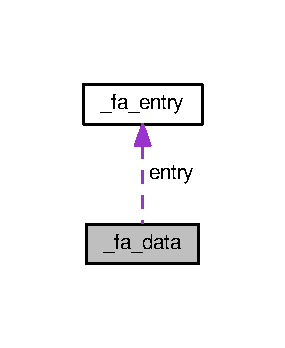
\includegraphics[width=137pt]{struct__fa__data__coll__graph}
\end{center}
\end{figure}
\subsection*{Public Attributes}
\begin{DoxyCompactItemize}
\item 
uint64\+\_\+t \hyperlink{struct__fa__data_a49ac64b09307f73104bbf1e650f3c2c5}{nlines}
\item 
int \hyperlink{struct__fa__data_a2e49d8da3a888d7df62cd887367e2923}{nentries}
\item 
int \hyperlink{struct__fa__data_a3607f37f43d8b2f14ced6a93c6a444ff}{linelen}
\item 
uint64\+\_\+t $\ast$ \hyperlink{struct__fa__data_acdb54c828a0fbfe8b8851f5290afc16e}{entrylen}
\item 
\hyperlink{fa__read_8h_a8f68b28ad3a6c33fe1dd78d5ac044b30}{Fa\+\_\+entry} $\ast$ \hyperlink{struct__fa__data_a3c2c4488c834a828085df7b409d292e4}{entry}
\end{DoxyCompactItemize}


\subsection{Detailed Description}
stores sequences of a fasta file 

\subsection{Member Data Documentation}
\hypertarget{struct__fa__data_a3c2c4488c834a828085df7b409d292e4}{\index{\+\_\+fa\+\_\+data@{\+\_\+fa\+\_\+data}!entry@{entry}}
\index{entry@{entry}!\+\_\+fa\+\_\+data@{\+\_\+fa\+\_\+data}}
\subsubsection[{entry}]{\setlength{\rightskip}{0pt plus 5cm}{\bf Fa\+\_\+entry}$\ast$ \+\_\+fa\+\_\+data\+::entry}}\label{struct__fa__data_a3c2c4488c834a828085df7b409d292e4}
Array with fasta entries (see Fa\+\_\+entry) \hypertarget{struct__fa__data_acdb54c828a0fbfe8b8851f5290afc16e}{\index{\+\_\+fa\+\_\+data@{\+\_\+fa\+\_\+data}!entrylen@{entrylen}}
\index{entrylen@{entrylen}!\+\_\+fa\+\_\+data@{\+\_\+fa\+\_\+data}}
\subsubsection[{entrylen}]{\setlength{\rightskip}{0pt plus 5cm}uint64\+\_\+t$\ast$ \+\_\+fa\+\_\+data\+::entrylen}}\label{struct__fa__data_acdb54c828a0fbfe8b8851f5290afc16e}
Array containing the length of the entries \hypertarget{struct__fa__data_a3607f37f43d8b2f14ced6a93c6a444ff}{\index{\+\_\+fa\+\_\+data@{\+\_\+fa\+\_\+data}!linelen@{linelen}}
\index{linelen@{linelen}!\+\_\+fa\+\_\+data@{\+\_\+fa\+\_\+data}}
\subsubsection[{linelen}]{\setlength{\rightskip}{0pt plus 5cm}int \+\_\+fa\+\_\+data\+::linelen}}\label{struct__fa__data_a3607f37f43d8b2f14ced6a93c6a444ff}
Line length of the $\ast$fa file entries \hypertarget{struct__fa__data_a2e49d8da3a888d7df62cd887367e2923}{\index{\+\_\+fa\+\_\+data@{\+\_\+fa\+\_\+data}!nentries@{nentries}}
\index{nentries@{nentries}!\+\_\+fa\+\_\+data@{\+\_\+fa\+\_\+data}}
\subsubsection[{nentries}]{\setlength{\rightskip}{0pt plus 5cm}int \+\_\+fa\+\_\+data\+::nentries}}\label{struct__fa__data_a2e49d8da3a888d7df62cd887367e2923}
Number of entries in $\ast$fa file \hypertarget{struct__fa__data_a49ac64b09307f73104bbf1e650f3c2c5}{\index{\+\_\+fa\+\_\+data@{\+\_\+fa\+\_\+data}!nlines@{nlines}}
\index{nlines@{nlines}!\+\_\+fa\+\_\+data@{\+\_\+fa\+\_\+data}}
\subsubsection[{nlines}]{\setlength{\rightskip}{0pt plus 5cm}uint64\+\_\+t \+\_\+fa\+\_\+data\+::nlines}}\label{struct__fa__data_a49ac64b09307f73104bbf1e650f3c2c5}
Number of lines in $\ast$fa file 

The documentation for this struct was generated from the following file\+:\begin{DoxyCompactItemize}
\item 
include/\hyperlink{fa__read_8h}{fa\+\_\+read.\+h}\end{DoxyCompactItemize}

\hypertarget{struct__fa__entry}{}\section{\+\_\+fa\+\_\+entry Struct Reference}
\label{struct__fa__entry}\index{\+\_\+fa\+\_\+entry@{\+\_\+fa\+\_\+entry}}


fasta entry  




{\ttfamily \#include $<$fa\+\_\+read.\+h$>$}

\subsection*{Public Attributes}
\begin{DoxyCompactItemize}
\item 
uint64\+\_\+t \mbox{\hyperlink{struct__fa__entry_a46bfe034cc419f00fccd2d7d174c76e2}{N}}
\item 
char $\ast$ \mbox{\hyperlink{struct__fa__entry_a6c548e86ed6ce8bb33bd1fcdcd56abbe}{seq}}
\end{DoxyCompactItemize}


\subsection{Detailed Description}
fasta entry 

\subsection{Member Data Documentation}
\mbox{\Hypertarget{struct__fa__entry_a46bfe034cc419f00fccd2d7d174c76e2}\label{struct__fa__entry_a46bfe034cc419f00fccd2d7d174c76e2}} 
\index{\+\_\+fa\+\_\+entry@{\+\_\+fa\+\_\+entry}!N@{N}}
\index{N@{N}!\+\_\+fa\+\_\+entry@{\+\_\+fa\+\_\+entry}}
\subsubsection{\texorpdfstring{N}{N}}
{\footnotesize\ttfamily uint64\+\_\+t \+\_\+fa\+\_\+entry\+::N}

Entry length (chars) \mbox{\Hypertarget{struct__fa__entry_a6c548e86ed6ce8bb33bd1fcdcd56abbe}\label{struct__fa__entry_a6c548e86ed6ce8bb33bd1fcdcd56abbe}} 
\index{\+\_\+fa\+\_\+entry@{\+\_\+fa\+\_\+entry}!seq@{seq}}
\index{seq@{seq}!\+\_\+fa\+\_\+entry@{\+\_\+fa\+\_\+entry}}
\subsubsection{\texorpdfstring{seq}{seq}}
{\footnotesize\ttfamily char$\ast$ \+\_\+fa\+\_\+entry\+::seq}

sequence 

The documentation for this struct was generated from the following file\+:\begin{DoxyCompactItemize}
\item 
include/\mbox{\hyperlink{fa__read_8h}{fa\+\_\+read.\+h}}\end{DoxyCompactItemize}

\hypertarget{struct__fq__read}{}\section{\+\_\+fq\+\_\+read Struct Reference}
\label{struct__fq__read}\index{\+\_\+fq\+\_\+read@{\+\_\+fq\+\_\+read}}


stores a fastq entry  




{\ttfamily \#include $<$fq\+\_\+read.\+h$>$}

\subsection*{Public Attributes}
\begin{DoxyCompactItemize}
\item 
char \mbox{\hyperlink{struct__fq__read_a7a643c49516b3a35f221d0fcda7f9ff3}{line1}} \mbox{[}R\+E\+A\+D\+\_\+\+M\+A\+X\+L\+EN\mbox{]}
\item 
char \mbox{\hyperlink{struct__fq__read_af2502a6f97e9508936c1b9f08890cc84}{line2}} \mbox{[}R\+E\+A\+D\+\_\+\+M\+A\+X\+L\+EN\mbox{]}
\item 
char \mbox{\hyperlink{struct__fq__read_a3df48e8dc31e47dc36c371002dba1bb5}{line3}} \mbox{[}R\+E\+A\+D\+\_\+\+M\+A\+X\+L\+EN\mbox{]}
\item 
char \mbox{\hyperlink{struct__fq__read_a8074fd734cb7e3d4b87454417aea569a}{line4}} \mbox{[}R\+E\+A\+D\+\_\+\+M\+A\+X\+L\+EN\mbox{]}
\item 
int \mbox{\hyperlink{struct__fq__read_a746efa9093b5223e85ffb7274e7693ef}{L}}
\item 
int \mbox{\hyperlink{struct__fq__read_a0b8deb6c25c72026b4928b17e3f12ade}{start}}
\item 
int \mbox{\hyperlink{struct__fq__read_a9cf08b81f1e78553e08fb597d30192b6}{Lhalf}}
\item 
char \mbox{\hyperlink{struct__fq__read_aae3ecb937cbba51f91baa391d8d84826}{extended}} \mbox{[}R\+E\+A\+D\+\_\+\+M\+A\+X\+L\+EN\mbox{]}
\item 
unsigned char \mbox{\hyperlink{struct__fq__read_afd023930012710b1a015ef78a02b3721}{pack}} \mbox{[}(R\+E\+A\+D\+\_\+\+M\+A\+X\+L\+EN+1)/2\mbox{]}
\item 
unsigned char \mbox{\hyperlink{struct__fq__read_a8c9786c5779078561abe5ec2e06c7ff9}{packsh}} \mbox{[}(R\+E\+A\+D\+\_\+\+M\+A\+X\+L\+EN+1)/2\mbox{]}
\item 
int \mbox{\hyperlink{struct__fq__read_a61c338fcae059e8581b02ec1b2cdcdc6}{L\+\_\+ad}}
\item 
int \mbox{\hyperlink{struct__fq__read_acf9a80768c42f71a975d602058e2ab52}{L\+\_\+ext}}
\item 
int \mbox{\hyperlink{struct__fq__read_a84f64405e7a9bbc055dd4f5534041782}{L\+\_\+pack}}
\item 
int \mbox{\hyperlink{struct__fq__read_a1303e633bdb4a7e31083d849a92fcbcc}{L\+\_\+packsh}}
\end{DoxyCompactItemize}


\subsection{Detailed Description}
stores a fastq entry 

\subsection{Member Data Documentation}
\mbox{\Hypertarget{struct__fq__read_aae3ecb937cbba51f91baa391d8d84826}\label{struct__fq__read_aae3ecb937cbba51f91baa391d8d84826}} 
\index{\+\_\+fq\+\_\+read@{\+\_\+fq\+\_\+read}!extended@{extended}}
\index{extended@{extended}!\+\_\+fq\+\_\+read@{\+\_\+fq\+\_\+read}}
\subsubsection{\texorpdfstring{extended}{extended}}
{\footnotesize\ttfamily char \+\_\+fq\+\_\+read\+::extended\mbox{[}R\+E\+A\+D\+\_\+\+M\+A\+X\+L\+EN\mbox{]}}

extended sequence, adapter added to 5\textquotesingle{} end \mbox{\Hypertarget{struct__fq__read_a746efa9093b5223e85ffb7274e7693ef}\label{struct__fq__read_a746efa9093b5223e85ffb7274e7693ef}} 
\index{\+\_\+fq\+\_\+read@{\+\_\+fq\+\_\+read}!L@{L}}
\index{L@{L}!\+\_\+fq\+\_\+read@{\+\_\+fq\+\_\+read}}
\subsubsection{\texorpdfstring{L}{L}}
{\footnotesize\ttfamily int \+\_\+fq\+\_\+read\+::L}

read length \mbox{\Hypertarget{struct__fq__read_a61c338fcae059e8581b02ec1b2cdcdc6}\label{struct__fq__read_a61c338fcae059e8581b02ec1b2cdcdc6}} 
\index{\+\_\+fq\+\_\+read@{\+\_\+fq\+\_\+read}!L\+\_\+ad@{L\+\_\+ad}}
\index{L\+\_\+ad@{L\+\_\+ad}!\+\_\+fq\+\_\+read@{\+\_\+fq\+\_\+read}}
\subsubsection{\texorpdfstring{L\+\_\+ad}{L\_ad}}
{\footnotesize\ttfamily int \+\_\+fq\+\_\+read\+::\+L\+\_\+ad}

length of adapter sequence \mbox{\Hypertarget{struct__fq__read_acf9a80768c42f71a975d602058e2ab52}\label{struct__fq__read_acf9a80768c42f71a975d602058e2ab52}} 
\index{\+\_\+fq\+\_\+read@{\+\_\+fq\+\_\+read}!L\+\_\+ext@{L\+\_\+ext}}
\index{L\+\_\+ext@{L\+\_\+ext}!\+\_\+fq\+\_\+read@{\+\_\+fq\+\_\+read}}
\subsubsection{\texorpdfstring{L\+\_\+ext}{L\_ext}}
{\footnotesize\ttfamily int \+\_\+fq\+\_\+read\+::\+L\+\_\+ext}

length of extended sequence \mbox{\Hypertarget{struct__fq__read_a84f64405e7a9bbc055dd4f5534041782}\label{struct__fq__read_a84f64405e7a9bbc055dd4f5534041782}} 
\index{\+\_\+fq\+\_\+read@{\+\_\+fq\+\_\+read}!L\+\_\+pack@{L\+\_\+pack}}
\index{L\+\_\+pack@{L\+\_\+pack}!\+\_\+fq\+\_\+read@{\+\_\+fq\+\_\+read}}
\subsubsection{\texorpdfstring{L\+\_\+pack}{L\_pack}}
{\footnotesize\ttfamily int \+\_\+fq\+\_\+read\+::\+L\+\_\+pack}

length of packed sequence \mbox{\Hypertarget{struct__fq__read_a1303e633bdb4a7e31083d849a92fcbcc}\label{struct__fq__read_a1303e633bdb4a7e31083d849a92fcbcc}} 
\index{\+\_\+fq\+\_\+read@{\+\_\+fq\+\_\+read}!L\+\_\+packsh@{L\+\_\+packsh}}
\index{L\+\_\+packsh@{L\+\_\+packsh}!\+\_\+fq\+\_\+read@{\+\_\+fq\+\_\+read}}
\subsubsection{\texorpdfstring{L\+\_\+packsh}{L\_packsh}}
{\footnotesize\ttfamily int \+\_\+fq\+\_\+read\+::\+L\+\_\+packsh}

length of packed sequence (shifted) \mbox{\Hypertarget{struct__fq__read_a9cf08b81f1e78553e08fb597d30192b6}\label{struct__fq__read_a9cf08b81f1e78553e08fb597d30192b6}} 
\index{\+\_\+fq\+\_\+read@{\+\_\+fq\+\_\+read}!Lhalf@{Lhalf}}
\index{Lhalf@{Lhalf}!\+\_\+fq\+\_\+read@{\+\_\+fq\+\_\+read}}
\subsubsection{\texorpdfstring{Lhalf}{Lhalf}}
{\footnotesize\ttfamily int \+\_\+fq\+\_\+read\+::\+Lhalf}

half of read length \mbox{\Hypertarget{struct__fq__read_a7a643c49516b3a35f221d0fcda7f9ff3}\label{struct__fq__read_a7a643c49516b3a35f221d0fcda7f9ff3}} 
\index{\+\_\+fq\+\_\+read@{\+\_\+fq\+\_\+read}!line1@{line1}}
\index{line1@{line1}!\+\_\+fq\+\_\+read@{\+\_\+fq\+\_\+read}}
\subsubsection{\texorpdfstring{line1}{line1}}
{\footnotesize\ttfamily char \+\_\+fq\+\_\+read\+::line1\mbox{[}R\+E\+A\+D\+\_\+\+M\+A\+X\+L\+EN\mbox{]}}

Line 1 in fastq entry \mbox{\Hypertarget{struct__fq__read_af2502a6f97e9508936c1b9f08890cc84}\label{struct__fq__read_af2502a6f97e9508936c1b9f08890cc84}} 
\index{\+\_\+fq\+\_\+read@{\+\_\+fq\+\_\+read}!line2@{line2}}
\index{line2@{line2}!\+\_\+fq\+\_\+read@{\+\_\+fq\+\_\+read}}
\subsubsection{\texorpdfstring{line2}{line2}}
{\footnotesize\ttfamily char \+\_\+fq\+\_\+read\+::line2\mbox{[}R\+E\+A\+D\+\_\+\+M\+A\+X\+L\+EN\mbox{]}}

Line 2 in fastq entry \mbox{\Hypertarget{struct__fq__read_a3df48e8dc31e47dc36c371002dba1bb5}\label{struct__fq__read_a3df48e8dc31e47dc36c371002dba1bb5}} 
\index{\+\_\+fq\+\_\+read@{\+\_\+fq\+\_\+read}!line3@{line3}}
\index{line3@{line3}!\+\_\+fq\+\_\+read@{\+\_\+fq\+\_\+read}}
\subsubsection{\texorpdfstring{line3}{line3}}
{\footnotesize\ttfamily char \+\_\+fq\+\_\+read\+::line3\mbox{[}R\+E\+A\+D\+\_\+\+M\+A\+X\+L\+EN\mbox{]}}

Line 3 in fastq entry \mbox{\Hypertarget{struct__fq__read_a8074fd734cb7e3d4b87454417aea569a}\label{struct__fq__read_a8074fd734cb7e3d4b87454417aea569a}} 
\index{\+\_\+fq\+\_\+read@{\+\_\+fq\+\_\+read}!line4@{line4}}
\index{line4@{line4}!\+\_\+fq\+\_\+read@{\+\_\+fq\+\_\+read}}
\subsubsection{\texorpdfstring{line4}{line4}}
{\footnotesize\ttfamily char \+\_\+fq\+\_\+read\+::line4\mbox{[}R\+E\+A\+D\+\_\+\+M\+A\+X\+L\+EN\mbox{]}}

Line 4 in fastq entry \mbox{\Hypertarget{struct__fq__read_afd023930012710b1a015ef78a02b3721}\label{struct__fq__read_afd023930012710b1a015ef78a02b3721}} 
\index{\+\_\+fq\+\_\+read@{\+\_\+fq\+\_\+read}!pack@{pack}}
\index{pack@{pack}!\+\_\+fq\+\_\+read@{\+\_\+fq\+\_\+read}}
\subsubsection{\texorpdfstring{pack}{pack}}
{\footnotesize\ttfamily unsigned char \+\_\+fq\+\_\+read\+::pack\mbox{[}(R\+E\+A\+D\+\_\+\+M\+A\+X\+L\+EN+1)/2\mbox{]}}

pack sequence \mbox{\Hypertarget{struct__fq__read_a8c9786c5779078561abe5ec2e06c7ff9}\label{struct__fq__read_a8c9786c5779078561abe5ec2e06c7ff9}} 
\index{\+\_\+fq\+\_\+read@{\+\_\+fq\+\_\+read}!packsh@{packsh}}
\index{packsh@{packsh}!\+\_\+fq\+\_\+read@{\+\_\+fq\+\_\+read}}
\subsubsection{\texorpdfstring{packsh}{packsh}}
{\footnotesize\ttfamily unsigned char \+\_\+fq\+\_\+read\+::packsh\mbox{[}(R\+E\+A\+D\+\_\+\+M\+A\+X\+L\+EN+1)/2\mbox{]}}

pack sequence with shift \mbox{\Hypertarget{struct__fq__read_a0b8deb6c25c72026b4928b17e3f12ade}\label{struct__fq__read_a0b8deb6c25c72026b4928b17e3f12ade}} 
\index{\+\_\+fq\+\_\+read@{\+\_\+fq\+\_\+read}!start@{start}}
\index{start@{start}!\+\_\+fq\+\_\+read@{\+\_\+fq\+\_\+read}}
\subsubsection{\texorpdfstring{start}{start}}
{\footnotesize\ttfamily int \+\_\+fq\+\_\+read\+::start}

nucleotide position start. Can only be different from zero if the read has been filtered with this tool. 

The documentation for this struct was generated from the following file\+:\begin{DoxyCompactItemize}
\item 
include/\mbox{\hyperlink{fq__read_8h}{fq\+\_\+read.\+h}}\end{DoxyCompactItemize}

\hypertarget{struct__iparam__Freport}{\section{\+\_\+iparam\+\_\+\+Freport Struct Reference}
\label{struct__iparam__Freport}\index{\+\_\+iparam\+\_\+\+Freport@{\+\_\+iparam\+\_\+\+Freport}}
}


contains Freport input parameters  




{\ttfamily \#include $<$init\+\_\+\+Freport.\+h$>$}

\subsection*{Public Attributes}
\begin{DoxyCompactItemize}
\item 
char $\ast$ \hyperlink{struct__iparam__Freport_a0e65baa185928cd40bb6aabb14c0f189}{inputfolder}
\item 
char \hyperlink{struct__iparam__Freport_a5c86fdc95e6c199dede6c269b8ea1417}{outputfile} \mbox{[}\hyperlink{defines_8h_abe0ec333b60117063f9b9fd9f849cb08}{M\+A\+X\+\_\+\+F\+I\+L\+E\+N\+A\+M\+E}\mbox{]}
\end{DoxyCompactItemize}


\subsection{Detailed Description}
contains Freport input parameters 

\subsection{Member Data Documentation}
\hypertarget{struct__iparam__Freport_a0e65baa185928cd40bb6aabb14c0f189}{\index{\+\_\+iparam\+\_\+\+Freport@{\+\_\+iparam\+\_\+\+Freport}!inputfolder@{inputfolder}}
\index{inputfolder@{inputfolder}!\+\_\+iparam\+\_\+\+Freport@{\+\_\+iparam\+\_\+\+Freport}}
\subsubsection[{inputfolder}]{\setlength{\rightskip}{0pt plus 5cm}char$\ast$ \+\_\+iparam\+\_\+\+Freport\+::inputfolder}}\label{struct__iparam__Freport_a0e65baa185928cd40bb6aabb14c0f189}
input folder \hypertarget{struct__iparam__Freport_a5c86fdc95e6c199dede6c269b8ea1417}{\index{\+\_\+iparam\+\_\+\+Freport@{\+\_\+iparam\+\_\+\+Freport}!outputfile@{outputfile}}
\index{outputfile@{outputfile}!\+\_\+iparam\+\_\+\+Freport@{\+\_\+iparam\+\_\+\+Freport}}
\subsubsection[{outputfile}]{\setlength{\rightskip}{0pt plus 5cm}char \+\_\+iparam\+\_\+\+Freport\+::outputfile\mbox{[}{\bf M\+A\+X\+\_\+\+F\+I\+L\+E\+N\+A\+M\+E}\mbox{]}}}\label{struct__iparam__Freport_a5c86fdc95e6c199dede6c269b8ea1417}
html outputfile name 

The documentation for this struct was generated from the following file\+:\begin{DoxyCompactItemize}
\item 
include/\hyperlink{init__Freport_8h}{init\+\_\+\+Freport.\+h}\end{DoxyCompactItemize}

\hypertarget{struct__iparam__makeTree}{\section{\+\_\+iparam\+\_\+make\+Tree Struct Reference}
\label{struct__iparam__makeTree}\index{\+\_\+iparam\+\_\+make\+Tree@{\+\_\+iparam\+\_\+make\+Tree}}
}


contains make\+Tree input parameters  




{\ttfamily \#include $<$init\+\_\+make\+Tree.\+h$>$}

\subsection*{Public Attributes}
\begin{DoxyCompactItemize}
\item 
char $\ast$ \hyperlink{struct__iparam__makeTree_a864d463534785b7f6cc7b9d52664b443}{inputfasta}
\item 
char \hyperlink{struct__iparam__makeTree_a9506dbea307f1fda5cc22c84bc4d035f}{outputfile} \mbox{[}\hyperlink{defines_8h_abe0ec333b60117063f9b9fd9f849cb08}{M\+A\+X\+\_\+\+F\+I\+L\+E\+N\+A\+M\+E}\mbox{]}
\item 
int \hyperlink{struct__iparam__makeTree_a56fd13b9cf051d4770f40b015a295fd3}{L}
\end{DoxyCompactItemize}


\subsection{Detailed Description}
contains make\+Tree input parameters 

\subsection{Member Data Documentation}
\hypertarget{struct__iparam__makeTree_a864d463534785b7f6cc7b9d52664b443}{\index{\+\_\+iparam\+\_\+make\+Tree@{\+\_\+iparam\+\_\+make\+Tree}!inputfasta@{inputfasta}}
\index{inputfasta@{inputfasta}!\+\_\+iparam\+\_\+make\+Tree@{\+\_\+iparam\+\_\+make\+Tree}}
\subsubsection[{inputfasta}]{\setlength{\rightskip}{0pt plus 5cm}char$\ast$ \+\_\+iparam\+\_\+make\+Tree\+::inputfasta}}\label{struct__iparam__makeTree_a864d463534785b7f6cc7b9d52664b443}
fasta input file \hypertarget{struct__iparam__makeTree_a56fd13b9cf051d4770f40b015a295fd3}{\index{\+\_\+iparam\+\_\+make\+Tree@{\+\_\+iparam\+\_\+make\+Tree}!L@{L}}
\index{L@{L}!\+\_\+iparam\+\_\+make\+Tree@{\+\_\+iparam\+\_\+make\+Tree}}
\subsubsection[{L}]{\setlength{\rightskip}{0pt plus 5cm}int \+\_\+iparam\+\_\+make\+Tree\+::\+L}}\label{struct__iparam__makeTree_a56fd13b9cf051d4770f40b015a295fd3}
tree depth \hypertarget{struct__iparam__makeTree_a9506dbea307f1fda5cc22c84bc4d035f}{\index{\+\_\+iparam\+\_\+make\+Tree@{\+\_\+iparam\+\_\+make\+Tree}!outputfile@{outputfile}}
\index{outputfile@{outputfile}!\+\_\+iparam\+\_\+make\+Tree@{\+\_\+iparam\+\_\+make\+Tree}}
\subsubsection[{outputfile}]{\setlength{\rightskip}{0pt plus 5cm}char \+\_\+iparam\+\_\+make\+Tree\+::outputfile\mbox{[}{\bf M\+A\+X\+\_\+\+F\+I\+L\+E\+N\+A\+M\+E}\mbox{]}}}\label{struct__iparam__makeTree_a9506dbea307f1fda5cc22c84bc4d035f}
outputfile path 

The documentation for this struct was generated from the following file\+:\begin{DoxyCompactItemize}
\item 
include/\hyperlink{init__makeTree_8h}{init\+\_\+make\+Tree.\+h}\end{DoxyCompactItemize}

\hypertarget{struct__iparam__Qreport}{\section{\+\_\+iparam\+\_\+\+Qreport Struct Reference}
\label{struct__iparam__Qreport}\index{\+\_\+iparam\+\_\+\+Qreport@{\+\_\+iparam\+\_\+\+Qreport}}
}


contains Qreport input parameters  




{\ttfamily \#include $<$init\+\_\+\+Qreport.\+h$>$}

\subsection*{Public Attributes}
\begin{DoxyCompactItemize}
\item 
char $\ast$ \hyperlink{struct__iparam__Qreport_ac96f6463d81dc1fcc41850564f24cf11}{inputfile}
\item 
char \hyperlink{struct__iparam__Qreport_abdf92f14bc1c49787cda4b94ceb668cd}{outputfilebin} \mbox{[}\hyperlink{defines_8h_abe0ec333b60117063f9b9fd9f849cb08}{M\+A\+X\+\_\+\+F\+I\+L\+E\+N\+A\+M\+E}\mbox{]}
\item 
char \hyperlink{struct__iparam__Qreport_a54ffbb27584db445494af7d9a1c214de}{outputfilehtml} \mbox{[}\hyperlink{defines_8h_abe0ec333b60117063f9b9fd9f849cb08}{M\+A\+X\+\_\+\+F\+I\+L\+E\+N\+A\+M\+E}\mbox{]}
\item 
char \hyperlink{struct__iparam__Qreport_a75f5c38f9365c0c1370040928f43d316}{outputfileinfo} \mbox{[}\hyperlink{defines_8h_abe0ec333b60117063f9b9fd9f849cb08}{M\+A\+X\+\_\+\+F\+I\+L\+E\+N\+A\+M\+E}\mbox{]}
\item 
int \hyperlink{struct__iparam__Qreport_a47cfa018e6e957cb132e22876a400a1f}{n\+Q}
\item 
int \hyperlink{struct__iparam__Qreport_a9d91db490f318f69dcea4999f630712e}{ntiles}
\item 
int \hyperlink{struct__iparam__Qreport_a1fa54b38e988ffe30eba5e0284e9dacb}{min\+Q}
\item 
int \hyperlink{struct__iparam__Qreport_a1004bab2a5776669710b74925ba4d338}{read\+\_\+len}
\item 
int \hyperlink{struct__iparam__Qreport_ae1ce417a16c5d30c05a09ec868154e14}{filter}
\item 
int \hyperlink{struct__iparam__Qreport_a0a09c5cc791e625b948acb45b39164e6}{one\+\_\+read\+\_\+len}
\end{DoxyCompactItemize}


\subsection{Detailed Description}
contains Qreport input parameters 

\subsection{Member Data Documentation}
\hypertarget{struct__iparam__Qreport_ae1ce417a16c5d30c05a09ec868154e14}{\index{\+\_\+iparam\+\_\+\+Qreport@{\+\_\+iparam\+\_\+\+Qreport}!filter@{filter}}
\index{filter@{filter}!\+\_\+iparam\+\_\+\+Qreport@{\+\_\+iparam\+\_\+\+Qreport}}
\subsubsection[{filter}]{\setlength{\rightskip}{0pt plus 5cm}int \+\_\+iparam\+\_\+\+Qreport\+::filter}}\label{struct__iparam__Qreport_ae1ce417a16c5d30c05a09ec868154e14}
0 original data, 1 this tool filtered data, 2 other tool filtered data \hypertarget{struct__iparam__Qreport_ac96f6463d81dc1fcc41850564f24cf11}{\index{\+\_\+iparam\+\_\+\+Qreport@{\+\_\+iparam\+\_\+\+Qreport}!inputfile@{inputfile}}
\index{inputfile@{inputfile}!\+\_\+iparam\+\_\+\+Qreport@{\+\_\+iparam\+\_\+\+Qreport}}
\subsubsection[{inputfile}]{\setlength{\rightskip}{0pt plus 5cm}char$\ast$ \+\_\+iparam\+\_\+\+Qreport\+::inputfile}}\label{struct__iparam__Qreport_ac96f6463d81dc1fcc41850564f24cf11}
Inputfile name \hypertarget{struct__iparam__Qreport_a1fa54b38e988ffe30eba5e0284e9dacb}{\index{\+\_\+iparam\+\_\+\+Qreport@{\+\_\+iparam\+\_\+\+Qreport}!min\+Q@{min\+Q}}
\index{min\+Q@{min\+Q}!\+\_\+iparam\+\_\+\+Qreport@{\+\_\+iparam\+\_\+\+Qreport}}
\subsubsection[{min\+Q}]{\setlength{\rightskip}{0pt plus 5cm}int \+\_\+iparam\+\_\+\+Qreport\+::min\+Q}}\label{struct__iparam__Qreport_a1fa54b38e988ffe30eba5e0284e9dacb}
minimum Quality allowed 0 -\/ 45 \hypertarget{struct__iparam__Qreport_a47cfa018e6e957cb132e22876a400a1f}{\index{\+\_\+iparam\+\_\+\+Qreport@{\+\_\+iparam\+\_\+\+Qreport}!n\+Q@{n\+Q}}
\index{n\+Q@{n\+Q}!\+\_\+iparam\+\_\+\+Qreport@{\+\_\+iparam\+\_\+\+Qreport}}
\subsubsection[{n\+Q}]{\setlength{\rightskip}{0pt plus 5cm}int \+\_\+iparam\+\_\+\+Qreport\+::n\+Q}}\label{struct__iparam__Qreport_a47cfa018e6e957cb132e22876a400a1f}
\# different quality values (default is 46) \hypertarget{struct__iparam__Qreport_a9d91db490f318f69dcea4999f630712e}{\index{\+\_\+iparam\+\_\+\+Qreport@{\+\_\+iparam\+\_\+\+Qreport}!ntiles@{ntiles}}
\index{ntiles@{ntiles}!\+\_\+iparam\+\_\+\+Qreport@{\+\_\+iparam\+\_\+\+Qreport}}
\subsubsection[{ntiles}]{\setlength{\rightskip}{0pt plus 5cm}int \+\_\+iparam\+\_\+\+Qreport\+::ntiles}}\label{struct__iparam__Qreport_a9d91db490f318f69dcea4999f630712e}
\# tiles (default is 96) \hypertarget{struct__iparam__Qreport_a0a09c5cc791e625b948acb45b39164e6}{\index{\+\_\+iparam\+\_\+\+Qreport@{\+\_\+iparam\+\_\+\+Qreport}!one\+\_\+read\+\_\+len@{one\+\_\+read\+\_\+len}}
\index{one\+\_\+read\+\_\+len@{one\+\_\+read\+\_\+len}!\+\_\+iparam\+\_\+\+Qreport@{\+\_\+iparam\+\_\+\+Qreport}}
\subsubsection[{one\+\_\+read\+\_\+len}]{\setlength{\rightskip}{0pt plus 5cm}int \+\_\+iparam\+\_\+\+Qreport\+::one\+\_\+read\+\_\+len}}\label{struct__iparam__Qreport_a0a09c5cc791e625b948acb45b39164e6}
1 all reads of equal length 0 reads have different lengths. \hypertarget{struct__iparam__Qreport_abdf92f14bc1c49787cda4b94ceb668cd}{\index{\+\_\+iparam\+\_\+\+Qreport@{\+\_\+iparam\+\_\+\+Qreport}!outputfilebin@{outputfilebin}}
\index{outputfilebin@{outputfilebin}!\+\_\+iparam\+\_\+\+Qreport@{\+\_\+iparam\+\_\+\+Qreport}}
\subsubsection[{outputfilebin}]{\setlength{\rightskip}{0pt plus 5cm}char \+\_\+iparam\+\_\+\+Qreport\+::outputfilebin\mbox{[}{\bf M\+A\+X\+\_\+\+F\+I\+L\+E\+N\+A\+M\+E}\mbox{]}}}\label{struct__iparam__Qreport_abdf92f14bc1c49787cda4b94ceb668cd}
Binary outputfile name. \hypertarget{struct__iparam__Qreport_a54ffbb27584db445494af7d9a1c214de}{\index{\+\_\+iparam\+\_\+\+Qreport@{\+\_\+iparam\+\_\+\+Qreport}!outputfilehtml@{outputfilehtml}}
\index{outputfilehtml@{outputfilehtml}!\+\_\+iparam\+\_\+\+Qreport@{\+\_\+iparam\+\_\+\+Qreport}}
\subsubsection[{outputfilehtml}]{\setlength{\rightskip}{0pt plus 5cm}char \+\_\+iparam\+\_\+\+Qreport\+::outputfilehtml\mbox{[}{\bf M\+A\+X\+\_\+\+F\+I\+L\+E\+N\+A\+M\+E}\mbox{]}}}\label{struct__iparam__Qreport_a54ffbb27584db445494af7d9a1c214de}
html outputfile name \hypertarget{struct__iparam__Qreport_a75f5c38f9365c0c1370040928f43d316}{\index{\+\_\+iparam\+\_\+\+Qreport@{\+\_\+iparam\+\_\+\+Qreport}!outputfileinfo@{outputfileinfo}}
\index{outputfileinfo@{outputfileinfo}!\+\_\+iparam\+\_\+\+Qreport@{\+\_\+iparam\+\_\+\+Qreport}}
\subsubsection[{outputfileinfo}]{\setlength{\rightskip}{0pt plus 5cm}char \+\_\+iparam\+\_\+\+Qreport\+::outputfileinfo\mbox{[}{\bf M\+A\+X\+\_\+\+F\+I\+L\+E\+N\+A\+M\+E}\mbox{]}}}\label{struct__iparam__Qreport_a75f5c38f9365c0c1370040928f43d316}
Info outputfile name \hypertarget{struct__iparam__Qreport_a1004bab2a5776669710b74925ba4d338}{\index{\+\_\+iparam\+\_\+\+Qreport@{\+\_\+iparam\+\_\+\+Qreport}!read\+\_\+len@{read\+\_\+len}}
\index{read\+\_\+len@{read\+\_\+len}!\+\_\+iparam\+\_\+\+Qreport@{\+\_\+iparam\+\_\+\+Qreport}}
\subsubsection[{read\+\_\+len}]{\setlength{\rightskip}{0pt plus 5cm}int \+\_\+iparam\+\_\+\+Qreport\+::read\+\_\+len}}\label{struct__iparam__Qreport_a1004bab2a5776669710b74925ba4d338}
original read length 

The documentation for this struct was generated from the following file\+:\begin{DoxyCompactItemize}
\item 
include/\hyperlink{init__Qreport_8h}{init\+\_\+\+Qreport.\+h}\end{DoxyCompactItemize}

\hypertarget{struct__iparam__Sreport}{\section{\+\_\+iparam\+\_\+\+Sreport Struct Reference}
\label{struct__iparam__Sreport}\index{\+\_\+iparam\+\_\+\+Sreport@{\+\_\+iparam\+\_\+\+Sreport}}
}


contains Sreport input parameters  




{\ttfamily \#include $<$init\+\_\+\+Sreport.\+h$>$}

\subsection*{Public Attributes}
\begin{DoxyCompactItemize}
\item 
char $\ast$ \hyperlink{struct__iparam__Sreport_af5521a185f440566547b4b11b9fac6a4}{inputfolder}
\item 
char \hyperlink{struct__iparam__Sreport_aab71d9b5647daf65a8ba9ba6f7a35ee5}{outputfile} \mbox{[}\hyperlink{defines_8h_abe0ec333b60117063f9b9fd9f849cb08}{M\+A\+X\+\_\+\+F\+I\+L\+E\+N\+A\+M\+E}\mbox{]}
\end{DoxyCompactItemize}


\subsection{Detailed Description}
contains Sreport input parameters 

\subsection{Member Data Documentation}
\hypertarget{struct__iparam__Sreport_af5521a185f440566547b4b11b9fac6a4}{\index{\+\_\+iparam\+\_\+\+Sreport@{\+\_\+iparam\+\_\+\+Sreport}!inputfolder@{inputfolder}}
\index{inputfolder@{inputfolder}!\+\_\+iparam\+\_\+\+Sreport@{\+\_\+iparam\+\_\+\+Sreport}}
\subsubsection[{inputfolder}]{\setlength{\rightskip}{0pt plus 5cm}char$\ast$ \+\_\+iparam\+\_\+\+Sreport\+::inputfolder}}\label{struct__iparam__Sreport_af5521a185f440566547b4b11b9fac6a4}
input folder \hypertarget{struct__iparam__Sreport_aab71d9b5647daf65a8ba9ba6f7a35ee5}{\index{\+\_\+iparam\+\_\+\+Sreport@{\+\_\+iparam\+\_\+\+Sreport}!outputfile@{outputfile}}
\index{outputfile@{outputfile}!\+\_\+iparam\+\_\+\+Sreport@{\+\_\+iparam\+\_\+\+Sreport}}
\subsubsection[{outputfile}]{\setlength{\rightskip}{0pt plus 5cm}char \+\_\+iparam\+\_\+\+Sreport\+::outputfile\mbox{[}{\bf M\+A\+X\+\_\+\+F\+I\+L\+E\+N\+A\+M\+E}\mbox{]}}}\label{struct__iparam__Sreport_aab71d9b5647daf65a8ba9ba6f7a35ee5}
html outputfile name 

The documentation for this struct was generated from the following file\+:\begin{DoxyCompactItemize}
\item 
include/\hyperlink{init__Sreport_8h}{init\+\_\+\+Sreport.\+h}\end{DoxyCompactItemize}

\hypertarget{struct__iparam__trimFilter}{\section{\+\_\+iparam\+\_\+trim\+Filter Struct Reference}
\label{struct__iparam__trimFilter}\index{\+\_\+iparam\+\_\+trim\+Filter@{\+\_\+iparam\+\_\+trim\+Filter}}
}
\subsection*{Public Attributes}
\begin{DoxyCompactItemize}
\item 
\hypertarget{struct__iparam__trimFilter_a5147310738277c148ca7109ba77829ca}{char $\ast$ {\bfseries Ifq}}\label{struct__iparam__trimFilter_a5147310738277c148ca7109ba77829ca}

\item 
\hypertarget{struct__iparam__trimFilter_a55796cd412ef4ca61a5a799d2f64beec}{char $\ast$ {\bfseries Ifa}}\label{struct__iparam__trimFilter_a55796cd412ef4ca61a5a799d2f64beec}

\item 
\hypertarget{struct__iparam__trimFilter_a158296e4d37ab3b033c6f9aee1516d71}{char $\ast$ {\bfseries Iidx}}\label{struct__iparam__trimFilter_a158296e4d37ab3b033c6f9aee1516d71}

\item 
\hypertarget{struct__iparam__trimFilter_ad24f2902b532a4ff2dfb1122941064b8}{char $\ast$ {\bfseries Oprefix}}\label{struct__iparam__trimFilter_ad24f2902b532a4ff2dfb1122941064b8}

\item 
\hypertarget{struct__iparam__trimFilter_a5b5344041c9313230de07c9485227203}{int {\bfseries trim\+Q}}\label{struct__iparam__trimFilter_a5b5344041c9313230de07c9485227203}

\item 
\hypertarget{struct__iparam__trimFilter_a5f2d247cc26608ed5cc9e2d6943940d7}{int {\bfseries trim\+N}}\label{struct__iparam__trimFilter_a5f2d247cc26608ed5cc9e2d6943940d7}

\item 
\hypertarget{struct__iparam__trimFilter_ac6093d26e41e61f82ffd2aa05f563f9c}{\hyperlink{defines_8h_abb452686968e48b67397da5f97445f5b}{bool} {\bfseries is\+\_\+fa}}\label{struct__iparam__trimFilter_ac6093d26e41e61f82ffd2aa05f563f9c}

\item 
\hypertarget{struct__iparam__trimFilter_afc50c477a3340ed7befc430d273ff6cb}{\hyperlink{defines_8h_abb452686968e48b67397da5f97445f5b}{bool} {\bfseries is\+\_\+idx}}\label{struct__iparam__trimFilter_afc50c477a3340ed7befc430d273ff6cb}

\item 
\hypertarget{struct__iparam__trimFilter_ac36acafc4290934f81444425f780deda}{\hyperlink{defines_8h_abb452686968e48b67397da5f97445f5b}{bool} {\bfseries tree}}\label{struct__iparam__trimFilter_ac36acafc4290934f81444425f780deda}

\item 
\hypertarget{struct__iparam__trimFilter_a193ef2030f6eb8db0b75afbbd152d6a1}{double {\bfseries score}}\label{struct__iparam__trimFilter_a193ef2030f6eb8db0b75afbbd152d6a1}

\item 
\hypertarget{struct__iparam__trimFilter_a1e2b69f148d9299815af6ab7f575ad1a}{int {\bfseries min\+Q}}\label{struct__iparam__trimFilter_a1e2b69f148d9299815af6ab7f575ad1a}

\item 
\hypertarget{struct__iparam__trimFilter_a72fcc236d4136d2405a04f155b515894}{int {\bfseries L}}\label{struct__iparam__trimFilter_a72fcc236d4136d2405a04f155b515894}

\item 
\hypertarget{struct__iparam__trimFilter_ac2b43664ca0c95a8572f97254893d675}{int {\bfseries min\+L}}\label{struct__iparam__trimFilter_ac2b43664ca0c95a8572f97254893d675}

\item 
\hypertarget{struct__iparam__trimFilter_aaeab85398303eada76cb6f32841fa094}{int {\bfseries nlow\+Q}}\label{struct__iparam__trimFilter_aaeab85398303eada76cb6f32841fa094}

\item 
\hypertarget{struct__iparam__trimFilter_a8d64cf4832f3c403bd7c505d5a3fee75}{int {\bfseries Lmer\+\_\+len}}\label{struct__iparam__trimFilter_a8d64cf4832f3c403bd7c505d5a3fee75}

\item 
\hypertarget{struct__iparam__trimFilter_a2e626c5776d4423d20d5ec7606fe9b81}{int {\bfseries globleft}}\label{struct__iparam__trimFilter_a2e626c5776d4423d20d5ec7606fe9b81}

\item 
\hypertarget{struct__iparam__trimFilter_ad5fb4ca1786b14cd63a8467187474f51}{int {\bfseries globright}}\label{struct__iparam__trimFilter_ad5fb4ca1786b14cd63a8467187474f51}

\item 
\hypertarget{struct__iparam__trimFilter_a8ed026b1de4fccc7288258c3a8faa395}{int {\bfseries percent}}\label{struct__iparam__trimFilter_a8ed026b1de4fccc7288258c3a8faa395}

\end{DoxyCompactItemize}


The documentation for this struct was generated from the following file\+:\begin{DoxyCompactItemize}
\item 
include/init\+\_\+trim\+Filter.\+h\end{DoxyCompactItemize}

\hypertarget{struct__node}{\section{\+\_\+node Struct Reference}
\label{struct__node}\index{\+\_\+node@{\+\_\+node}}
}


Node structure\+: formed out of T\+\_\+\+A\+C\+G\+T pointers to Node structure.  




{\ttfamily \#include $<$tree.\+h$>$}



Collaboration diagram for \+\_\+node\+:\nopagebreak
\begin{figure}[H]
\begin{center}
\leavevmode
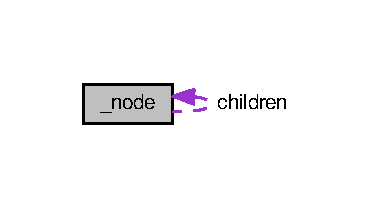
\includegraphics[width=178pt]{struct__node__coll__graph}
\end{center}
\end{figure}
\subsection*{Public Attributes}
\begin{DoxyCompactItemize}
\item 
struct \hyperlink{struct__node}{\+\_\+node} $\ast$ \hyperlink{struct__node_a7f878e5e9c5c9d2801715c870b9bbc1c}{children} \mbox{[}\hyperlink{defines_8h_a3919067d6defd46504313402bac82d22}{T\+\_\+\+A\+C\+G\+T}\mbox{]}
\end{DoxyCompactItemize}


\subsection{Detailed Description}
Node structure\+: formed out of T\+\_\+\+A\+C\+G\+T pointers to Node structure. 

\subsection{Member Data Documentation}
\hypertarget{struct__node_a7f878e5e9c5c9d2801715c870b9bbc1c}{\index{\+\_\+node@{\+\_\+node}!children@{children}}
\index{children@{children}!\+\_\+node@{\+\_\+node}}
\subsubsection[{children}]{\setlength{\rightskip}{0pt plus 5cm}struct {\bf \+\_\+node}$\ast$ \+\_\+node\+::children\mbox{[}{\bf T\+\_\+\+A\+C\+G\+T}\mbox{]}}}\label{struct__node_a7f878e5e9c5c9d2801715c870b9bbc1c}
T\+\_\+\+A\+C\+G\+T pointers to Node structure 

The documentation for this struct was generated from the following file\+:\begin{DoxyCompactItemize}
\item 
include/\hyperlink{tree_8h}{tree.\+h}\end{DoxyCompactItemize}

\hypertarget{struct__split}{}\section{\+\_\+split Struct Reference}
\label{struct__split}\index{\+\_\+split@{\+\_\+split}}


contains a splitted string and the number or splitted fields  




{\ttfamily \#include $<$str\+\_\+manip.\+h$>$}

\subsection*{Public Attributes}
\begin{DoxyCompactItemize}
\item 
int \mbox{\hyperlink{struct__split_af3261bd49762652bb67cc1e76300f582}{N}}
\item 
char $\ast$$\ast$ \mbox{\hyperlink{struct__split_a84d5273295857f35a812eeab15ae607f}{s}}
\end{DoxyCompactItemize}


\subsection{Detailed Description}
contains a splitted string and the number or splitted fields 

\subsection{Member Data Documentation}
\mbox{\Hypertarget{struct__split_af3261bd49762652bb67cc1e76300f582}\label{struct__split_af3261bd49762652bb67cc1e76300f582}} 
\index{\+\_\+split@{\+\_\+split}!N@{N}}
\index{N@{N}!\+\_\+split@{\+\_\+split}}
\subsubsection{\texorpdfstring{N}{N}}
{\footnotesize\ttfamily int \+\_\+split\+::N}

Number of substrings in which the string was splitted \mbox{\Hypertarget{struct__split_a84d5273295857f35a812eeab15ae607f}\label{struct__split_a84d5273295857f35a812eeab15ae607f}} 
\index{\+\_\+split@{\+\_\+split}!s@{s}}
\index{s@{s}!\+\_\+split@{\+\_\+split}}
\subsubsection{\texorpdfstring{s}{s}}
{\footnotesize\ttfamily char$\ast$$\ast$ \+\_\+split\+::s}

Substring array containing the splitted substrings 

The documentation for this struct was generated from the following file\+:\begin{DoxyCompactItemize}
\item 
include/\mbox{\hyperlink{str__manip_8h}{str\+\_\+manip.\+h}}\end{DoxyCompactItemize}

\hypertarget{struct__stats__TF}{\section{\+\_\+stats\+\_\+\+T\+F Struct Reference}
\label{struct__stats__TF}\index{\+\_\+stats\+\_\+\+T\+F@{\+\_\+stats\+\_\+\+T\+F}}
}


collects stats info from the filtering procedure  




{\ttfamily \#include $<$io\+\_\+trim\+Filter.\+h$>$}

\subsection*{Public Attributes}
\begin{DoxyCompactItemize}
\item 
int \hyperlink{struct__stats__TF_a47d4caef2878e2c10e7571cfdd2d9619}{filters} \mbox{[}\hyperlink{defines_8h_a23f1103d8247781ab0be4b0fba2f085f}{N\+F\+I\+L\+T\+E\+R\+S}\mbox{]}
\item 
int \hyperlink{struct__stats__TF_a399de2eb5fd452f019d5c8d23bae0651}{trimmed} \mbox{[}\hyperlink{defines_8h_a23f1103d8247781ab0be4b0fba2f085f}{N\+F\+I\+L\+T\+E\+R\+S}\mbox{]}
\item 
int \hyperlink{struct__stats__TF_a876a430dbbb78e3b03f9e7088da26618}{discarded} \mbox{[}\hyperlink{defines_8h_a23f1103d8247781ab0be4b0fba2f085f}{N\+F\+I\+L\+T\+E\+R\+S}\mbox{]}
\item 
int \hyperlink{struct__stats__TF_a4d36ddc878d561051a0f9464df2e0911}{good}
\item 
int \hyperlink{struct__stats__TF_a2a3993588191eb9f03416cce4fb1862f}{nreads}
\end{DoxyCompactItemize}


\subsection{Detailed Description}
collects stats info from the filtering procedure 

\subsection{Member Data Documentation}
\hypertarget{struct__stats__TF_a876a430dbbb78e3b03f9e7088da26618}{\index{\+\_\+stats\+\_\+\+T\+F@{\+\_\+stats\+\_\+\+T\+F}!discarded@{discarded}}
\index{discarded@{discarded}!\+\_\+stats\+\_\+\+T\+F@{\+\_\+stats\+\_\+\+T\+F}}
\subsubsection[{discarded}]{\setlength{\rightskip}{0pt plus 5cm}int \+\_\+stats\+\_\+\+T\+F\+::discarded\mbox{[}{\bf N\+F\+I\+L\+T\+E\+R\+S}\mbox{]}}}\label{struct__stats__TF_a876a430dbbb78e3b03f9e7088da26618}
\# discarded reads\+: A\+D\+A\+P, C\+O\+N\+T, L\+O\+W\+Q, N\+N\+N\+N \hypertarget{struct__stats__TF_a47d4caef2878e2c10e7571cfdd2d9619}{\index{\+\_\+stats\+\_\+\+T\+F@{\+\_\+stats\+\_\+\+T\+F}!filters@{filters}}
\index{filters@{filters}!\+\_\+stats\+\_\+\+T\+F@{\+\_\+stats\+\_\+\+T\+F}}
\subsubsection[{filters}]{\setlength{\rightskip}{0pt plus 5cm}int \+\_\+stats\+\_\+\+T\+F\+::filters\mbox{[}{\bf N\+F\+I\+L\+T\+E\+R\+S}\mbox{]}}}\label{struct__stats__TF_a47d4caef2878e2c10e7571cfdd2d9619}
Using filters for\+: A\+D\+A\+P, C\+O\+N\+T, L\+O\+W\+Q, N\+N\+N\+N \hypertarget{struct__stats__TF_a4d36ddc878d561051a0f9464df2e0911}{\index{\+\_\+stats\+\_\+\+T\+F@{\+\_\+stats\+\_\+\+T\+F}!good@{good}}
\index{good@{good}!\+\_\+stats\+\_\+\+T\+F@{\+\_\+stats\+\_\+\+T\+F}}
\subsubsection[{good}]{\setlength{\rightskip}{0pt plus 5cm}int \+\_\+stats\+\_\+\+T\+F\+::good}}\label{struct__stats__TF_a4d36ddc878d561051a0f9464df2e0911}
\# good reads \hypertarget{struct__stats__TF_a2a3993588191eb9f03416cce4fb1862f}{\index{\+\_\+stats\+\_\+\+T\+F@{\+\_\+stats\+\_\+\+T\+F}!nreads@{nreads}}
\index{nreads@{nreads}!\+\_\+stats\+\_\+\+T\+F@{\+\_\+stats\+\_\+\+T\+F}}
\subsubsection[{nreads}]{\setlength{\rightskip}{0pt plus 5cm}int \+\_\+stats\+\_\+\+T\+F\+::nreads}}\label{struct__stats__TF_a2a3993588191eb9f03416cce4fb1862f}
total number of reads in the fq file \hypertarget{struct__stats__TF_a399de2eb5fd452f019d5c8d23bae0651}{\index{\+\_\+stats\+\_\+\+T\+F@{\+\_\+stats\+\_\+\+T\+F}!trimmed@{trimmed}}
\index{trimmed@{trimmed}!\+\_\+stats\+\_\+\+T\+F@{\+\_\+stats\+\_\+\+T\+F}}
\subsubsection[{trimmed}]{\setlength{\rightskip}{0pt plus 5cm}int \+\_\+stats\+\_\+\+T\+F\+::trimmed\mbox{[}{\bf N\+F\+I\+L\+T\+E\+R\+S}\mbox{]}}}\label{struct__stats__TF_a399de2eb5fd452f019d5c8d23bae0651}
\# trimmed reads by\+: A\+D\+A\+P, C\+O\+N\+T, L\+O\+W\+Q, N\+N\+N\+N 

The documentation for this struct was generated from the following file\+:\begin{DoxyCompactItemize}
\item 
include/\hyperlink{io__trimFilter_8h}{io\+\_\+trim\+Filter.\+h}\end{DoxyCompactItemize}

\hypertarget{struct__tree}{\section{\+\_\+tree Struct Reference}
\label{struct__tree}\index{\+\_\+tree@{\+\_\+tree}}
}


structure containing a T\+\_\+\+A\+C\+G\+T-\/tree.  




{\ttfamily \#include $<$tree.\+h$>$}



Collaboration diagram for \+\_\+tree\+:\nopagebreak
\begin{figure}[H]
\begin{center}
\leavevmode
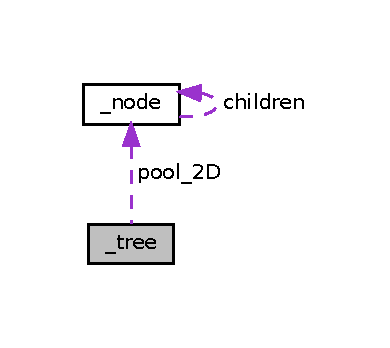
\includegraphics[width=178pt]{struct__tree__coll__graph}
\end{center}
\end{figure}
\subsection*{Public Attributes}
\begin{DoxyCompactItemize}
\item 
uint32\+\_\+t \hyperlink{struct__tree_a36ca6c909dd7c119452da0cb49e2c829}{L}
\item 
uint32\+\_\+t \hyperlink{struct__tree_aa90c2b558fc833fc22bcd6617689a41f}{pool\+\_\+count}
\item 
uint32\+\_\+t \hyperlink{struct__tree_afd3769cd9db40fa460d35a0033fb7d02}{pool\+\_\+available}
\item 
uint32\+\_\+t \hyperlink{struct__tree_abffdcd9dcf0df92df4b5444fb74cc523}{nnodes}
\item 
\hyperlink{tree_8h_a6390a1d02010dee1843fa2b1263308c1}{Node} $\ast$$\ast$ \hyperlink{struct__tree_a2783a2aaf32fc3b3c9de8b9fbb14de58}{pool\+\_\+2\+D}
\end{DoxyCompactItemize}


\subsection{Detailed Description}
structure containing a T\+\_\+\+A\+C\+G\+T-\/tree. 

The tree structure is stored in a pointer to pointer to Node. We grow the structure on the flight as we need more memory. In the outer direction, we start by allocating N\+P\+O\+O\+L\+\_\+2\+D pointers to Node. In the inner direction, we allocate N\+P\+O\+O\+L\+\_\+1\+D Nodes and fill them as we read the fasta file. When all of them are allocated, we allocate again N\+P\+O\+O\+L\+\_\+1\+D. If N\+P\+O\+O\+L\+\_\+2\+D pointers to Node are allocated, the outer dimension is reallocated with +\+N\+P\+O\+O\+L\+\_\+2\+D extra elements. L is the depth of the tree, pool\+\_\+count is the number on Node$\ast$ elements used so far, pool\+\_\+available is the number of Nodes available in every moment, and nnodes is the total number of nodes filled in. We limit the number of allocated nodes to U\+I\+N\+T\+\_\+\+M\+A\+X (we cannot count more nodes!). 

\subsection{Member Data Documentation}
\hypertarget{struct__tree_a36ca6c909dd7c119452da0cb49e2c829}{\index{\+\_\+tree@{\+\_\+tree}!L@{L}}
\index{L@{L}!\+\_\+tree@{\+\_\+tree}}
\subsubsection[{L}]{\setlength{\rightskip}{0pt plus 5cm}uint32\+\_\+t \+\_\+tree\+::\+L}}\label{struct__tree_a36ca6c909dd7c119452da0cb49e2c829}
depth of the tree \hypertarget{struct__tree_abffdcd9dcf0df92df4b5444fb74cc523}{\index{\+\_\+tree@{\+\_\+tree}!nnodes@{nnodes}}
\index{nnodes@{nnodes}!\+\_\+tree@{\+\_\+tree}}
\subsubsection[{nnodes}]{\setlength{\rightskip}{0pt plus 5cm}uint32\+\_\+t \+\_\+tree\+::nnodes}}\label{struct__tree_abffdcd9dcf0df92df4b5444fb74cc523}
Number of nodes in the tree \hypertarget{struct__tree_a2783a2aaf32fc3b3c9de8b9fbb14de58}{\index{\+\_\+tree@{\+\_\+tree}!pool\+\_\+2\+D@{pool\+\_\+2\+D}}
\index{pool\+\_\+2\+D@{pool\+\_\+2\+D}!\+\_\+tree@{\+\_\+tree}}
\subsubsection[{pool\+\_\+2\+D}]{\setlength{\rightskip}{0pt plus 5cm}{\bf Node}$\ast$$\ast$ \+\_\+tree\+::pool\+\_\+2\+D}}\label{struct__tree_a2783a2aaf32fc3b3c9de8b9fbb14de58}
2\+D pool containing the nodes that form the tree \hypertarget{struct__tree_afd3769cd9db40fa460d35a0033fb7d02}{\index{\+\_\+tree@{\+\_\+tree}!pool\+\_\+available@{pool\+\_\+available}}
\index{pool\+\_\+available@{pool\+\_\+available}!\+\_\+tree@{\+\_\+tree}}
\subsubsection[{pool\+\_\+available}]{\setlength{\rightskip}{0pt plus 5cm}uint32\+\_\+t \+\_\+tree\+::pool\+\_\+available}}\label{struct__tree_afd3769cd9db40fa460d35a0033fb7d02}
Number of empty nodes available in the pool \hypertarget{struct__tree_aa90c2b558fc833fc22bcd6617689a41f}{\index{\+\_\+tree@{\+\_\+tree}!pool\+\_\+count@{pool\+\_\+count}}
\index{pool\+\_\+count@{pool\+\_\+count}!\+\_\+tree@{\+\_\+tree}}
\subsubsection[{pool\+\_\+count}]{\setlength{\rightskip}{0pt plus 5cm}uint32\+\_\+t \+\_\+tree\+::pool\+\_\+count}}\label{struct__tree_aa90c2b558fc833fc22bcd6617689a41f}
Number of elements in the second dimension 

The documentation for this struct was generated from the following file\+:\begin{DoxyCompactItemize}
\item 
include/\hyperlink{tree_8h}{tree.\+h}\end{DoxyCompactItemize}

\hypertarget{structstatsinfo}{\section{statsinfo Struct Reference}
\label{structstatsinfo}\index{statsinfo@{statsinfo}}
}


stores info needed to create the summary graphs  




{\ttfamily \#include $<$stats\+\_\+info.\+h$>$}

\subsection*{Public Attributes}
\begin{DoxyCompactItemize}
\item 
int \hyperlink{structstatsinfo_a90c9a180632378e22ab9b0358daf3f0d}{read\+\_\+len}
\item 
int \hyperlink{structstatsinfo_abcfe8e12737ac99b724d4d4407204ec8}{ntiles}
\item 
int \hyperlink{structstatsinfo_a8f99f5ac1c3643e6ad59f124c11676e2}{n\+Q}
\item 
int \hyperlink{structstatsinfo_a6b33794a27827b8e2ea2b45a95f937d9}{min\+Q}
\item 
int \hyperlink{structstatsinfo_a740378fa01d92f6e0b2c50a26889fefd}{tile\+\_\+pos}
\item 
int \hyperlink{structstatsinfo_a2f01e91b444793507cb4173582e215bb}{nreads}
\item 
int \hyperlink{structstatsinfo_a14bb0b9848f2301718833bd2130683b7}{reads\+\_\+w\+N}
\item 
int \hyperlink{structstatsinfo_ae3c83d12e46748f3a0de4628b5e48068}{sz\+\_\+low\+Q\+\_\+\+A\+C\+G\+T\+\_\+tile}
\item 
int \hyperlink{structstatsinfo_a4e1223289cbb8f609d522747d4b47b54}{sz\+\_\+\+A\+C\+G\+T\+\_\+tile}
\item 
int \hyperlink{structstatsinfo_a5f0e812f7a2213cb57a79c8110b7a02e}{sz\+\_\+reads\+\_\+\+Mlow\+Q}
\item 
int \hyperlink{structstatsinfo_aceed3737e42259fa6e7438dc185e587f}{sz\+\_\+\+Q\+Pos\+Tile\+\_\+table}
\item 
int \hyperlink{structstatsinfo_ae95899480cc574a09163190663dd504a}{sz\+\_\+\+A\+C\+G\+T\+\_\+pos}
\item 
int $\ast$ \hyperlink{structstatsinfo_a25f475c79fa4d5aa1255b8c543d8a731}{tile\+\_\+tags}
\item 
int $\ast$ \hyperlink{structstatsinfo_a2fc74c1d7cec79d9b28b5e578d96d7a1}{lane\+\_\+tags}
\item 
int $\ast$ \hyperlink{structstatsinfo_a2fc7cfbe32bd01653402ff070638292b}{qual\+\_\+tags}
\item 
uint64\+\_\+t $\ast$ \hyperlink{structstatsinfo_ac1a8b88e2e4f486f2767072588adcd2a}{low\+Q\+\_\+\+A\+C\+G\+T\+\_\+tile}
\item 
uint64\+\_\+t $\ast$ \hyperlink{structstatsinfo_aa4987d17317a2d744efaa104f7a3e0b7}{A\+C\+G\+T\+\_\+tile}
\item 
uint64\+\_\+t $\ast$ \hyperlink{structstatsinfo_a9b58ee91e10fa9301a186ca94e68e6fb}{reads\+\_\+\+Mlow\+Q}
\item 
uint64\+\_\+t $\ast$ \hyperlink{structstatsinfo_af2781fc5113bab8c208921a221e2c834}{Q\+Pos\+Tile\+\_\+table}
\item 
uint64\+\_\+t $\ast$ \hyperlink{structstatsinfo_a315b402bd89ea205117d2fab4b26ef10}{A\+C\+G\+T\+\_\+pos}
\end{DoxyCompactItemize}


\subsection{Detailed Description}
stores info needed to create the summary graphs 

\subsection{Member Data Documentation}
\hypertarget{structstatsinfo_a315b402bd89ea205117d2fab4b26ef10}{\index{statsinfo@{statsinfo}!A\+C\+G\+T\+\_\+pos@{A\+C\+G\+T\+\_\+pos}}
\index{A\+C\+G\+T\+\_\+pos@{A\+C\+G\+T\+\_\+pos}!statsinfo@{statsinfo}}
\subsubsection[{A\+C\+G\+T\+\_\+pos}]{\setlength{\rightskip}{0pt plus 5cm}uint64\+\_\+t$\ast$ statsinfo\+::\+A\+C\+G\+T\+\_\+pos}}\label{structstatsinfo_a315b402bd89ea205117d2fab4b26ef10}
\# A, C, G, T, N per position \hypertarget{structstatsinfo_aa4987d17317a2d744efaa104f7a3e0b7}{\index{statsinfo@{statsinfo}!A\+C\+G\+T\+\_\+tile@{A\+C\+G\+T\+\_\+tile}}
\index{A\+C\+G\+T\+\_\+tile@{A\+C\+G\+T\+\_\+tile}!statsinfo@{statsinfo}}
\subsubsection[{A\+C\+G\+T\+\_\+tile}]{\setlength{\rightskip}{0pt plus 5cm}uint64\+\_\+t$\ast$ statsinfo\+::\+A\+C\+G\+T\+\_\+tile}}\label{structstatsinfo_aa4987d17317a2d744efaa104f7a3e0b7}
\# A, C, G, T, N per tile, to compute the fraction of low\+Quality bases per tile and per nucleotide. \hypertarget{structstatsinfo_a2fc74c1d7cec79d9b28b5e578d96d7a1}{\index{statsinfo@{statsinfo}!lane\+\_\+tags@{lane\+\_\+tags}}
\index{lane\+\_\+tags@{lane\+\_\+tags}!statsinfo@{statsinfo}}
\subsubsection[{lane\+\_\+tags}]{\setlength{\rightskip}{0pt plus 5cm}int$\ast$ statsinfo\+::lane\+\_\+tags}}\label{structstatsinfo_a2fc74c1d7cec79d9b28b5e578d96d7a1}
Names of the existing tiles \hypertarget{structstatsinfo_ac1a8b88e2e4f486f2767072588adcd2a}{\index{statsinfo@{statsinfo}!low\+Q\+\_\+\+A\+C\+G\+T\+\_\+tile@{low\+Q\+\_\+\+A\+C\+G\+T\+\_\+tile}}
\index{low\+Q\+\_\+\+A\+C\+G\+T\+\_\+tile@{low\+Q\+\_\+\+A\+C\+G\+T\+\_\+tile}!statsinfo@{statsinfo}}
\subsubsection[{low\+Q\+\_\+\+A\+C\+G\+T\+\_\+tile}]{\setlength{\rightskip}{0pt plus 5cm}uint64\+\_\+t$\ast$ statsinfo\+::low\+Q\+\_\+\+A\+C\+G\+T\+\_\+tile}}\label{structstatsinfo_ac1a8b88e2e4f486f2767072588adcd2a}
\# low Quality A, C, G, T, N per tile \hypertarget{structstatsinfo_a6b33794a27827b8e2ea2b45a95f937d9}{\index{statsinfo@{statsinfo}!min\+Q@{min\+Q}}
\index{min\+Q@{min\+Q}!statsinfo@{statsinfo}}
\subsubsection[{min\+Q}]{\setlength{\rightskip}{0pt plus 5cm}int statsinfo\+::min\+Q}}\label{structstatsinfo_a6b33794a27827b8e2ea2b45a95f937d9}
Minimum quality threshold \hypertarget{structstatsinfo_a8f99f5ac1c3643e6ad59f124c11676e2}{\index{statsinfo@{statsinfo}!n\+Q@{n\+Q}}
\index{n\+Q@{n\+Q}!statsinfo@{statsinfo}}
\subsubsection[{n\+Q}]{\setlength{\rightskip}{0pt plus 5cm}int statsinfo\+::n\+Q}}\label{structstatsinfo_a8f99f5ac1c3643e6ad59f124c11676e2}
\# possible quality values \hypertarget{structstatsinfo_a2f01e91b444793507cb4173582e215bb}{\index{statsinfo@{statsinfo}!nreads@{nreads}}
\index{nreads@{nreads}!statsinfo@{statsinfo}}
\subsubsection[{nreads}]{\setlength{\rightskip}{0pt plus 5cm}int statsinfo\+::nreads}}\label{structstatsinfo_a2f01e91b444793507cb4173582e215bb}
\# reads read till current position. \hypertarget{structstatsinfo_abcfe8e12737ac99b724d4d4407204ec8}{\index{statsinfo@{statsinfo}!ntiles@{ntiles}}
\index{ntiles@{ntiles}!statsinfo@{statsinfo}}
\subsubsection[{ntiles}]{\setlength{\rightskip}{0pt plus 5cm}int statsinfo\+::ntiles}}\label{structstatsinfo_abcfe8e12737ac99b724d4d4407204ec8}
\# tiles \hypertarget{structstatsinfo_af2781fc5113bab8c208921a221e2c834}{\index{statsinfo@{statsinfo}!Q\+Pos\+Tile\+\_\+table@{Q\+Pos\+Tile\+\_\+table}}
\index{Q\+Pos\+Tile\+\_\+table@{Q\+Pos\+Tile\+\_\+table}!statsinfo@{statsinfo}}
\subsubsection[{Q\+Pos\+Tile\+\_\+table}]{\setlength{\rightskip}{0pt plus 5cm}uint64\+\_\+t$\ast$ statsinfo\+::\+Q\+Pos\+Tile\+\_\+table}}\label{structstatsinfo_af2781fc5113bab8c208921a221e2c834}
\# bases of a given quality per tile. \hypertarget{structstatsinfo_a2fc7cfbe32bd01653402ff070638292b}{\index{statsinfo@{statsinfo}!qual\+\_\+tags@{qual\+\_\+tags}}
\index{qual\+\_\+tags@{qual\+\_\+tags}!statsinfo@{statsinfo}}
\subsubsection[{qual\+\_\+tags}]{\setlength{\rightskip}{0pt plus 5cm}int$\ast$ statsinfo\+::qual\+\_\+tags}}\label{structstatsinfo_a2fc7cfbe32bd01653402ff070638292b}
Names of the existing qualities \hypertarget{structstatsinfo_a90c9a180632378e22ab9b0358daf3f0d}{\index{statsinfo@{statsinfo}!read\+\_\+len@{read\+\_\+len}}
\index{read\+\_\+len@{read\+\_\+len}!statsinfo@{statsinfo}}
\subsubsection[{read\+\_\+len}]{\setlength{\rightskip}{0pt plus 5cm}int statsinfo\+::read\+\_\+len}}\label{structstatsinfo_a90c9a180632378e22ab9b0358daf3f0d}
Maximum length of a read \hypertarget{structstatsinfo_a9b58ee91e10fa9301a186ca94e68e6fb}{\index{statsinfo@{statsinfo}!reads\+\_\+\+Mlow\+Q@{reads\+\_\+\+Mlow\+Q}}
\index{reads\+\_\+\+Mlow\+Q@{reads\+\_\+\+Mlow\+Q}!statsinfo@{statsinfo}}
\subsubsection[{reads\+\_\+\+Mlow\+Q}]{\setlength{\rightskip}{0pt plus 5cm}uint64\+\_\+t$\ast$ statsinfo\+::reads\+\_\+\+Mlow\+Q}}\label{structstatsinfo_a9b58ee91e10fa9301a186ca94e68e6fb}
\# reads with M(position) low\+Quality bases. \hypertarget{structstatsinfo_a14bb0b9848f2301718833bd2130683b7}{\index{statsinfo@{statsinfo}!reads\+\_\+w\+N@{reads\+\_\+w\+N}}
\index{reads\+\_\+w\+N@{reads\+\_\+w\+N}!statsinfo@{statsinfo}}
\subsubsection[{reads\+\_\+w\+N}]{\setlength{\rightskip}{0pt plus 5cm}int statsinfo\+::reads\+\_\+w\+N}}\label{structstatsinfo_a14bb0b9848f2301718833bd2130683b7}
\# reads with N's found till current position \hypertarget{structstatsinfo_ae95899480cc574a09163190663dd504a}{\index{statsinfo@{statsinfo}!sz\+\_\+\+A\+C\+G\+T\+\_\+pos@{sz\+\_\+\+A\+C\+G\+T\+\_\+pos}}
\index{sz\+\_\+\+A\+C\+G\+T\+\_\+pos@{sz\+\_\+\+A\+C\+G\+T\+\_\+pos}!statsinfo@{statsinfo}}
\subsubsection[{sz\+\_\+\+A\+C\+G\+T\+\_\+pos}]{\setlength{\rightskip}{0pt plus 5cm}int statsinfo\+::sz\+\_\+\+A\+C\+G\+T\+\_\+pos}}\label{structstatsinfo_ae95899480cc574a09163190663dd504a}
A\+C\+G\+T\+\_\+pos size = read\+\_\+len $\ast$ N\+\_\+\+A\+C\+G\+T \hypertarget{structstatsinfo_a4e1223289cbb8f609d522747d4b47b54}{\index{statsinfo@{statsinfo}!sz\+\_\+\+A\+C\+G\+T\+\_\+tile@{sz\+\_\+\+A\+C\+G\+T\+\_\+tile}}
\index{sz\+\_\+\+A\+C\+G\+T\+\_\+tile@{sz\+\_\+\+A\+C\+G\+T\+\_\+tile}!statsinfo@{statsinfo}}
\subsubsection[{sz\+\_\+\+A\+C\+G\+T\+\_\+tile}]{\setlength{\rightskip}{0pt plus 5cm}int statsinfo\+::sz\+\_\+\+A\+C\+G\+T\+\_\+tile}}\label{structstatsinfo_a4e1223289cbb8f609d522747d4b47b54}
A\+C\+G\+T\+\_\+tile size = ntiles $\ast$ N\+A\+C\+G\+T \hypertarget{structstatsinfo_ae3c83d12e46748f3a0de4628b5e48068}{\index{statsinfo@{statsinfo}!sz\+\_\+low\+Q\+\_\+\+A\+C\+G\+T\+\_\+tile@{sz\+\_\+low\+Q\+\_\+\+A\+C\+G\+T\+\_\+tile}}
\index{sz\+\_\+low\+Q\+\_\+\+A\+C\+G\+T\+\_\+tile@{sz\+\_\+low\+Q\+\_\+\+A\+C\+G\+T\+\_\+tile}!statsinfo@{statsinfo}}
\subsubsection[{sz\+\_\+low\+Q\+\_\+\+A\+C\+G\+T\+\_\+tile}]{\setlength{\rightskip}{0pt plus 5cm}int statsinfo\+::sz\+\_\+low\+Q\+\_\+\+A\+C\+G\+T\+\_\+tile}}\label{structstatsinfo_ae3c83d12e46748f3a0de4628b5e48068}
low\+Q\+\_\+\+A\+C\+G\+T\+\_\+tile size = ntiles $\ast$ N\+\_\+\+A\+C\+G\+T \hypertarget{structstatsinfo_aceed3737e42259fa6e7438dc185e587f}{\index{statsinfo@{statsinfo}!sz\+\_\+\+Q\+Pos\+Tile\+\_\+table@{sz\+\_\+\+Q\+Pos\+Tile\+\_\+table}}
\index{sz\+\_\+\+Q\+Pos\+Tile\+\_\+table@{sz\+\_\+\+Q\+Pos\+Tile\+\_\+table}!statsinfo@{statsinfo}}
\subsubsection[{sz\+\_\+\+Q\+Pos\+Tile\+\_\+table}]{\setlength{\rightskip}{0pt plus 5cm}int statsinfo\+::sz\+\_\+\+Q\+Pos\+Tile\+\_\+table}}\label{structstatsinfo_aceed3737e42259fa6e7438dc185e587f}
Qpos\+Tile\+\_\+\+Table size = ntiles $\ast$ n\+Q $\ast$ read\+\_\+len \hypertarget{structstatsinfo_a5f0e812f7a2213cb57a79c8110b7a02e}{\index{statsinfo@{statsinfo}!sz\+\_\+reads\+\_\+\+Mlow\+Q@{sz\+\_\+reads\+\_\+\+Mlow\+Q}}
\index{sz\+\_\+reads\+\_\+\+Mlow\+Q@{sz\+\_\+reads\+\_\+\+Mlow\+Q}!statsinfo@{statsinfo}}
\subsubsection[{sz\+\_\+reads\+\_\+\+Mlow\+Q}]{\setlength{\rightskip}{0pt plus 5cm}int statsinfo\+::sz\+\_\+reads\+\_\+\+Mlow\+Q}}\label{structstatsinfo_a5f0e812f7a2213cb57a79c8110b7a02e}
reads\+\_\+\+Mlow\+Q size = read\+\_\+len + 1 \hypertarget{structstatsinfo_a740378fa01d92f6e0b2c50a26889fefd}{\index{statsinfo@{statsinfo}!tile\+\_\+pos@{tile\+\_\+pos}}
\index{tile\+\_\+pos@{tile\+\_\+pos}!statsinfo@{statsinfo}}
\subsubsection[{tile\+\_\+pos}]{\setlength{\rightskip}{0pt plus 5cm}int statsinfo\+::tile\+\_\+pos}}\label{structstatsinfo_a740378fa01d92f6e0b2c50a26889fefd}
current tile position \hypertarget{structstatsinfo_a25f475c79fa4d5aa1255b8c543d8a731}{\index{statsinfo@{statsinfo}!tile\+\_\+tags@{tile\+\_\+tags}}
\index{tile\+\_\+tags@{tile\+\_\+tags}!statsinfo@{statsinfo}}
\subsubsection[{tile\+\_\+tags}]{\setlength{\rightskip}{0pt plus 5cm}int$\ast$ statsinfo\+::tile\+\_\+tags}}\label{structstatsinfo_a25f475c79fa4d5aa1255b8c543d8a731}
Names of the existing tiles 

The documentation for this struct was generated from the following file\+:\begin{DoxyCompactItemize}
\item 
include/\hyperlink{stats__info_8h}{stats\+\_\+info.\+h}\end{DoxyCompactItemize}

\chapter{File Documentation}
\hypertarget{defines_8h}{\section{include/defines.h File Reference}
\label{defines_8h}\index{include/defines.\+h@{include/defines.\+h}}
}


Macro definitions.  


This graph shows which files directly or indirectly include this file\+:\nopagebreak
\begin{figure}[H]
\begin{center}
\leavevmode
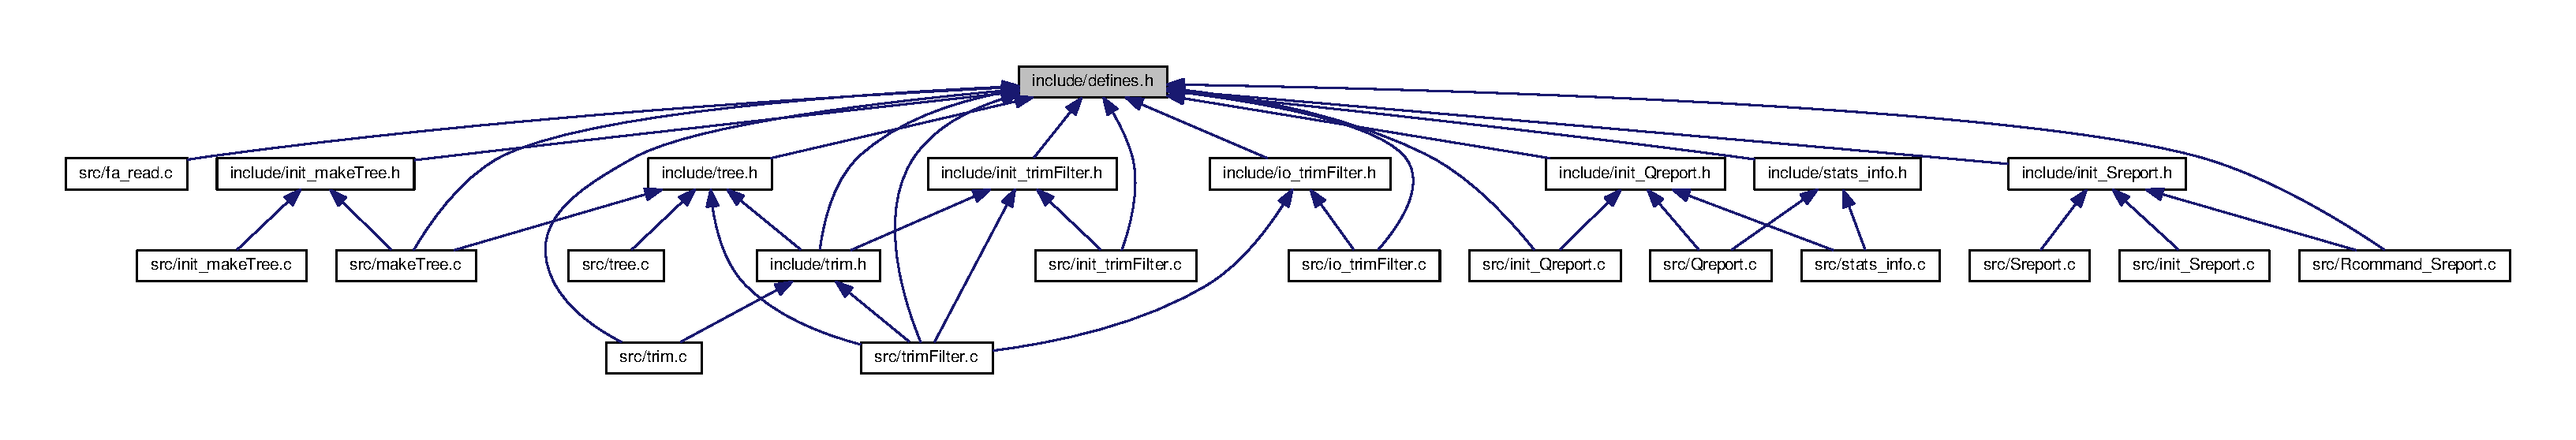
\includegraphics[width=350pt]{defines_8h__dep__incl}
\end{center}
\end{figure}
\subsection*{Macros}
\begin{DoxyCompactItemize}
\item 
\#define \hyperlink{defines_8h_a4419cb9bb22330d00cfd4727a05060dd}{B\+\_\+\+L\+E\+N}~131072
\item 
\#define \hyperlink{defines_8h_abe0ec333b60117063f9b9fd9f849cb08}{M\+A\+X\+\_\+\+F\+I\+L\+E\+N\+A\+M\+E}~300
\item 
\#define \hyperlink{defines_8h_abb452686968e48b67397da5f97445f5b}{bool}~short
\item 
\#define \hyperlink{defines_8h_a41f9c5fb8b08eb5dc3edce4dcb37fee7}{true}~1
\item 
\#define \hyperlink{defines_8h_a65e9886d74aaee76545e83dd09011727}{false}~0
\item 
\#define \hyperlink{defines_8h_affe776513b24d84b39af8ab0930fef7f}{max}(a, b)~( ((a) $>$ (b)) ? (a) \+: (b) )
\item 
\#define \hyperlink{defines_8h_ac6afabdc09a49a433ee19d8a9486056d}{min}(a, b)~( ((a) $<$ (b)) ? (a) \+: (b) )
\item 
\#define \hyperlink{defines_8h_afb615637083826bc311382f50b9a112d}{mem\+\_\+usage\+M\+B}()
\item 
\#define \hyperlink{defines_8h_a3589a26d6b84700042e948056edb43f6}{mem\+\_\+usage}()
\item 
\#define \hyperlink{defines_8h_a5c35b08af4e6a3b09783354fcd255b79}{D\+E\+F\+A\+U\+L\+T\+\_\+\+M\+I\+N\+Q}~27
\item 
\#define \hyperlink{defines_8h_ad27320ae41ed8a200b4379d022dd3d2e}{D\+E\+F\+A\+U\+L\+T\+\_\+\+N\+T\+I\+L\+E\+S}~96
\item 
\#define \hyperlink{defines_8h_afc545fae88ff3e374926c51cc44ff4e1}{D\+E\+F\+A\+U\+L\+T\+\_\+\+N\+Q}~46
\item 
\#define \hyperlink{defines_8h_aa98062065af56c6cd07cc43f35ef7aad}{Z\+E\+R\+O\+Q}~33
\item 
\#define \hyperlink{defines_8h_a71b6eab2a5d9fd457d48f50869a888f6}{N\+\_\+\+A\+C\+G\+T}~5
\item 
\#define \hyperlink{defines_8h_ac95fc8ee3f8ffd70f4564bcdc813ae2d}{M\+A\+X\+\_\+\+R\+C\+O\+M\+M\+A\+N\+D}~4000
\item 
\#define \hyperlink{defines_8h_a305c0ce0ef65658d5c81329adf54294f}{F\+A\+\_\+\+E\+N\+T\+R\+Y\+\_\+\+B\+U\+F}~20
\item 
\#define \hyperlink{defines_8h_a3919067d6defd46504313402bac82d22}{T\+\_\+\+A\+C\+G\+T}~4
\item 
\#define \hyperlink{defines_8h_a4d1f3741d002e1c5367ca1e87ee103ae}{N\+P\+O\+O\+L\+\_\+1\+D}~1048576
\item 
\#define \hyperlink{defines_8h_aaaa0c4d9e8b67e3f38fb68b27baca056}{N\+P\+O\+O\+L\+\_\+2\+D}~16
\item 
\#define \hyperlink{defines_8h_aba3b47d51c7ee08d2e0e92e58aa07106}{M\+A\+X\+\_\+\+F\+A\+S\+Z\+\_\+\+T\+R\+E\+E}~1e7
\item 
\#define \hyperlink{defines_8h_acd2baa2e68a76c64752672c201fff29a}{B\+I\+T\+S\+P\+E\+R\+C\+H\+A\+R}~8
\item 
\#define \hyperlink{defines_8h_a6722ebf83f6f843343b21592e3cd86ed}{B\+A\+S\+E\+S\+P\+E\+R\+C\+H\+A\+R}~4
\item 
\#define \hyperlink{defines_8h_a53c139d8ab18ed3e13ff65f63067fcac}{K\+M\+E\+R\+\_\+\+L\+E\+N}~25
\item 
\#define \hyperlink{defines_8h_ad9cbfc308e2064d4cc62c835753a39ea}{F\+A\+L\+S\+E\+\_\+\+P\+O\+S\+\_\+\+R\+A\+T\+E}~0.\+05
\item 
\#define \hyperlink{defines_8h_a78ea345c3971e9f004f71b15dda31d37}{Z\+E\+R\+O\+\_\+\+P\+O\+S\+\_\+\+R\+A\+T\+E}~1e-\/14
\item 
\#define \hyperlink{defines_8h_a996bde01ecac342918f0a2c4e7ce7bd5}{N\+O}~0
\item 
\#define \hyperlink{defines_8h_a1edd1ea8bddaf4d9c5eb3eae1ee1726a}{A\+L\+L}~1
\item 
\#define \hyperlink{defines_8h_a052e72209cfac2ff9aa78294f0bebea8}{E\+N\+D\+S}~2
\item 
\#define \hyperlink{defines_8h_a53529d9638a1d70f6e5989dedf4c2672}{S\+T\+R\+I\+P}~3
\item 
\#define \hyperlink{defines_8h_a653af6bd29f56a2699de26a928820da7}{F\+R\+A\+C}~3
\item 
\#define \hyperlink{defines_8h_abf0b71573c7ffc4f6746c24c9abc202a}{E\+N\+D\+S\+F\+R\+A\+C}~4
\item 
\#define \hyperlink{defines_8h_a3de33738fd3c7e77bffbcfaefc3e7645}{G\+L\+O\+B\+A\+L}~5
\item 
\#define \hyperlink{defines_8h_abf5b8fbbeb8255336e401a15a80214a8}{T\+R\+E\+E}~1
\item 
\#define \hyperlink{defines_8h_a1e43924adac4ae865aa0acf79710261c}{S\+A}~2
\item 
\#define \hyperlink{defines_8h_a7dcb6cfd9e186d997dce1d6cabe58898}{B\+L\+O\+O\+M}~3
\item 
\#define \hyperlink{defines_8h_a8fe83ac76edc595f6b98cd4a4127aed5}{E\+R\+R\+O\+R}~1000
\item 
\#define \hyperlink{defines_8h_a7fcff0e388619a194fb57f65c1053944}{D\+E\+F\+A\+U\+L\+T\+\_\+\+M\+I\+N\+L}~25
\item 
\#define \hyperlink{defines_8h_a50b2092be2f53229fda4d54644214af7}{A\+D\+A\+P}~0
\item 
\#define \hyperlink{defines_8h_a60519a721b44bce2b05a70cfa7ae8a1b}{C\+O\+N\+T}~1
\item 
\#define \hyperlink{defines_8h_a88236da90fdc203156cd02218f106f25}{L\+O\+W\+Q}~2
\item 
\#define \hyperlink{defines_8h_afdad8e3654b5f02ff4c50fcb88f6eed9}{N\+N\+N\+N}~3
\item 
\#define \hyperlink{defines_8h_a4adf7c6105c54a1608753548236d1387}{G\+O\+O\+D}~4
\item 
\#define \hyperlink{defines_8h_a23f1103d8247781ab0be4b0fba2f085f}{N\+F\+I\+L\+T\+E\+R\+S}~4
\end{DoxyCompactItemize}


\subsection{Detailed Description}
Macro definitions. 

\begin{DoxyAuthor}{Author}
Paula Perez \href{mailto:paulaperezrubio@gmail.com}{\tt paulaperezrubio@gmail.\+com} 
\end{DoxyAuthor}
\begin{DoxyDate}{Date}
07.\+08.\+2017 
\end{DoxyDate}


\subsection{Macro Definition Documentation}
\hypertarget{defines_8h_a50b2092be2f53229fda4d54644214af7}{\index{defines.\+h@{defines.\+h}!A\+D\+A\+P@{A\+D\+A\+P}}
\index{A\+D\+A\+P@{A\+D\+A\+P}!defines.\+h@{defines.\+h}}
\subsubsection[{A\+D\+A\+P}]{\setlength{\rightskip}{0pt plus 5cm}\#define A\+D\+A\+P~0}}\label{defines_8h_a50b2092be2f53229fda4d54644214af7}
Adapter filter \hypertarget{defines_8h_a1edd1ea8bddaf4d9c5eb3eae1ee1726a}{\index{defines.\+h@{defines.\+h}!A\+L\+L@{A\+L\+L}}
\index{A\+L\+L@{A\+L\+L}!defines.\+h@{defines.\+h}}
\subsubsection[{A\+L\+L}]{\setlength{\rightskip}{0pt plus 5cm}\#define A\+L\+L~1}}\label{defines_8h_a1edd1ea8bddaf4d9c5eb3eae1ee1726a}
Trims if a low\+Q base calling $\vert$ N is found \hypertarget{defines_8h_a4419cb9bb22330d00cfd4727a05060dd}{\index{defines.\+h@{defines.\+h}!B\+\_\+\+L\+E\+N@{B\+\_\+\+L\+E\+N}}
\index{B\+\_\+\+L\+E\+N@{B\+\_\+\+L\+E\+N}!defines.\+h@{defines.\+h}}
\subsubsection[{B\+\_\+\+L\+E\+N}]{\setlength{\rightskip}{0pt plus 5cm}\#define B\+\_\+\+L\+E\+N~131072}}\label{defines_8h_a4419cb9bb22330d00cfd4727a05060dd}
buffer size \hypertarget{defines_8h_a6722ebf83f6f843343b21592e3cd86ed}{\index{defines.\+h@{defines.\+h}!B\+A\+S\+E\+S\+P\+E\+R\+C\+H\+A\+R@{B\+A\+S\+E\+S\+P\+E\+R\+C\+H\+A\+R}}
\index{B\+A\+S\+E\+S\+P\+E\+R\+C\+H\+A\+R@{B\+A\+S\+E\+S\+P\+E\+R\+C\+H\+A\+R}!defines.\+h@{defines.\+h}}
\subsubsection[{B\+A\+S\+E\+S\+P\+E\+R\+C\+H\+A\+R}]{\setlength{\rightskip}{0pt plus 5cm}\#define B\+A\+S\+E\+S\+P\+E\+R\+C\+H\+A\+R~4}}\label{defines_8h_a6722ebf83f6f843343b21592e3cd86ed}
number of nucleotides that can fit in a char \hypertarget{defines_8h_acd2baa2e68a76c64752672c201fff29a}{\index{defines.\+h@{defines.\+h}!B\+I\+T\+S\+P\+E\+R\+C\+H\+A\+R@{B\+I\+T\+S\+P\+E\+R\+C\+H\+A\+R}}
\index{B\+I\+T\+S\+P\+E\+R\+C\+H\+A\+R@{B\+I\+T\+S\+P\+E\+R\+C\+H\+A\+R}!defines.\+h@{defines.\+h}}
\subsubsection[{B\+I\+T\+S\+P\+E\+R\+C\+H\+A\+R}]{\setlength{\rightskip}{0pt plus 5cm}\#define B\+I\+T\+S\+P\+E\+R\+C\+H\+A\+R~8}}\label{defines_8h_acd2baa2e68a76c64752672c201fff29a}
number of bits in a char \hypertarget{defines_8h_a7dcb6cfd9e186d997dce1d6cabe58898}{\index{defines.\+h@{defines.\+h}!B\+L\+O\+O\+M@{B\+L\+O\+O\+M}}
\index{B\+L\+O\+O\+M@{B\+L\+O\+O\+M}!defines.\+h@{defines.\+h}}
\subsubsection[{B\+L\+O\+O\+M}]{\setlength{\rightskip}{0pt plus 5cm}\#define B\+L\+O\+O\+M~3}}\label{defines_8h_a7dcb6cfd9e186d997dce1d6cabe58898}
Use a bloom filter to look for contaminations \hypertarget{defines_8h_abb452686968e48b67397da5f97445f5b}{\index{defines.\+h@{defines.\+h}!bool@{bool}}
\index{bool@{bool}!defines.\+h@{defines.\+h}}
\subsubsection[{bool}]{\setlength{\rightskip}{0pt plus 5cm}\#define bool~short}}\label{defines_8h_abb452686968e48b67397da5f97445f5b}
define a bool type \hypertarget{defines_8h_a60519a721b44bce2b05a70cfa7ae8a1b}{\index{defines.\+h@{defines.\+h}!C\+O\+N\+T@{C\+O\+N\+T}}
\index{C\+O\+N\+T@{C\+O\+N\+T}!defines.\+h@{defines.\+h}}
\subsubsection[{C\+O\+N\+T}]{\setlength{\rightskip}{0pt plus 5cm}\#define C\+O\+N\+T~1}}\label{defines_8h_a60519a721b44bce2b05a70cfa7ae8a1b}
Contamination filter \hypertarget{defines_8h_a7fcff0e388619a194fb57f65c1053944}{\index{defines.\+h@{defines.\+h}!D\+E\+F\+A\+U\+L\+T\+\_\+\+M\+I\+N\+L@{D\+E\+F\+A\+U\+L\+T\+\_\+\+M\+I\+N\+L}}
\index{D\+E\+F\+A\+U\+L\+T\+\_\+\+M\+I\+N\+L@{D\+E\+F\+A\+U\+L\+T\+\_\+\+M\+I\+N\+L}!defines.\+h@{defines.\+h}}
\subsubsection[{D\+E\+F\+A\+U\+L\+T\+\_\+\+M\+I\+N\+L}]{\setlength{\rightskip}{0pt plus 5cm}\#define D\+E\+F\+A\+U\+L\+T\+\_\+\+M\+I\+N\+L~25}}\label{defines_8h_a7fcff0e388619a194fb57f65c1053944}
Default minimum length under which we discard the reads \hypertarget{defines_8h_a5c35b08af4e6a3b09783354fcd255b79}{\index{defines.\+h@{defines.\+h}!D\+E\+F\+A\+U\+L\+T\+\_\+\+M\+I\+N\+Q@{D\+E\+F\+A\+U\+L\+T\+\_\+\+M\+I\+N\+Q}}
\index{D\+E\+F\+A\+U\+L\+T\+\_\+\+M\+I\+N\+Q@{D\+E\+F\+A\+U\+L\+T\+\_\+\+M\+I\+N\+Q}!defines.\+h@{defines.\+h}}
\subsubsection[{D\+E\+F\+A\+U\+L\+T\+\_\+\+M\+I\+N\+Q}]{\setlength{\rightskip}{0pt plus 5cm}\#define D\+E\+F\+A\+U\+L\+T\+\_\+\+M\+I\+N\+Q~27}}\label{defines_8h_a5c35b08af4e6a3b09783354fcd255b79}
Minimum quality threshold \hypertarget{defines_8h_afc545fae88ff3e374926c51cc44ff4e1}{\index{defines.\+h@{defines.\+h}!D\+E\+F\+A\+U\+L\+T\+\_\+\+N\+Q@{D\+E\+F\+A\+U\+L\+T\+\_\+\+N\+Q}}
\index{D\+E\+F\+A\+U\+L\+T\+\_\+\+N\+Q@{D\+E\+F\+A\+U\+L\+T\+\_\+\+N\+Q}!defines.\+h@{defines.\+h}}
\subsubsection[{D\+E\+F\+A\+U\+L\+T\+\_\+\+N\+Q}]{\setlength{\rightskip}{0pt plus 5cm}\#define D\+E\+F\+A\+U\+L\+T\+\_\+\+N\+Q~46}}\label{defines_8h_afc545fae88ff3e374926c51cc44ff4e1}
Default number of different quality values \hypertarget{defines_8h_ad27320ae41ed8a200b4379d022dd3d2e}{\index{defines.\+h@{defines.\+h}!D\+E\+F\+A\+U\+L\+T\+\_\+\+N\+T\+I\+L\+E\+S@{D\+E\+F\+A\+U\+L\+T\+\_\+\+N\+T\+I\+L\+E\+S}}
\index{D\+E\+F\+A\+U\+L\+T\+\_\+\+N\+T\+I\+L\+E\+S@{D\+E\+F\+A\+U\+L\+T\+\_\+\+N\+T\+I\+L\+E\+S}!defines.\+h@{defines.\+h}}
\subsubsection[{D\+E\+F\+A\+U\+L\+T\+\_\+\+N\+T\+I\+L\+E\+S}]{\setlength{\rightskip}{0pt plus 5cm}\#define D\+E\+F\+A\+U\+L\+T\+\_\+\+N\+T\+I\+L\+E\+S~96}}\label{defines_8h_ad27320ae41ed8a200b4379d022dd3d2e}
Default number of tiles \hypertarget{defines_8h_a052e72209cfac2ff9aa78294f0bebea8}{\index{defines.\+h@{defines.\+h}!E\+N\+D\+S@{E\+N\+D\+S}}
\index{E\+N\+D\+S@{E\+N\+D\+S}!defines.\+h@{defines.\+h}}
\subsubsection[{E\+N\+D\+S}]{\setlength{\rightskip}{0pt plus 5cm}\#define E\+N\+D\+S~2}}\label{defines_8h_a052e72209cfac2ff9aa78294f0bebea8}
Trims at the ends \hypertarget{defines_8h_abf0b71573c7ffc4f6746c24c9abc202a}{\index{defines.\+h@{defines.\+h}!E\+N\+D\+S\+F\+R\+A\+C@{E\+N\+D\+S\+F\+R\+A\+C}}
\index{E\+N\+D\+S\+F\+R\+A\+C@{E\+N\+D\+S\+F\+R\+A\+C}!defines.\+h@{defines.\+h}}
\subsubsection[{E\+N\+D\+S\+F\+R\+A\+C}]{\setlength{\rightskip}{0pt plus 5cm}\#define E\+N\+D\+S\+F\+R\+A\+C~4}}\label{defines_8h_abf0b71573c7ffc4f6746c24c9abc202a}
trims at the ends and discards a read if the remaining part has more than $>$ percent low\+Q bases \hypertarget{defines_8h_a8fe83ac76edc595f6b98cd4a4127aed5}{\index{defines.\+h@{defines.\+h}!E\+R\+R\+O\+R@{E\+R\+R\+O\+R}}
\index{E\+R\+R\+O\+R@{E\+R\+R\+O\+R}!defines.\+h@{defines.\+h}}
\subsubsection[{E\+R\+R\+O\+R}]{\setlength{\rightskip}{0pt plus 5cm}\#define E\+R\+R\+O\+R~1000}}\label{defines_8h_a8fe83ac76edc595f6b98cd4a4127aed5}
Encodes an error when reading in trim\+N, trim\+Q, method options in trim\+Filter \hypertarget{defines_8h_a305c0ce0ef65658d5c81329adf54294f}{\index{defines.\+h@{defines.\+h}!F\+A\+\_\+\+E\+N\+T\+R\+Y\+\_\+\+B\+U\+F@{F\+A\+\_\+\+E\+N\+T\+R\+Y\+\_\+\+B\+U\+F}}
\index{F\+A\+\_\+\+E\+N\+T\+R\+Y\+\_\+\+B\+U\+F@{F\+A\+\_\+\+E\+N\+T\+R\+Y\+\_\+\+B\+U\+F}!defines.\+h@{defines.\+h}}
\subsubsection[{F\+A\+\_\+\+E\+N\+T\+R\+Y\+\_\+\+B\+U\+F}]{\setlength{\rightskip}{0pt plus 5cm}\#define F\+A\+\_\+\+E\+N\+T\+R\+Y\+\_\+\+B\+U\+F~20}}\label{defines_8h_a305c0ce0ef65658d5c81329adf54294f}
buffer for fasta entries \hypertarget{defines_8h_a65e9886d74aaee76545e83dd09011727}{\index{defines.\+h@{defines.\+h}!false@{false}}
\index{false@{false}!defines.\+h@{defines.\+h}}
\subsubsection[{false}]{\setlength{\rightskip}{0pt plus 5cm}\#define false~0}}\label{defines_8h_a65e9886d74aaee76545e83dd09011727}
assign false to 0 \hypertarget{defines_8h_ad9cbfc308e2064d4cc62c835753a39ea}{\index{defines.\+h@{defines.\+h}!F\+A\+L\+S\+E\+\_\+\+P\+O\+S\+\_\+\+R\+A\+T\+E@{F\+A\+L\+S\+E\+\_\+\+P\+O\+S\+\_\+\+R\+A\+T\+E}}
\index{F\+A\+L\+S\+E\+\_\+\+P\+O\+S\+\_\+\+R\+A\+T\+E@{F\+A\+L\+S\+E\+\_\+\+P\+O\+S\+\_\+\+R\+A\+T\+E}!defines.\+h@{defines.\+h}}
\subsubsection[{F\+A\+L\+S\+E\+\_\+\+P\+O\+S\+\_\+\+R\+A\+T\+E}]{\setlength{\rightskip}{0pt plus 5cm}\#define F\+A\+L\+S\+E\+\_\+\+P\+O\+S\+\_\+\+R\+A\+T\+E~0.\+05}}\label{defines_8h_ad9cbfc308e2064d4cc62c835753a39ea}
default false positive rate \hypertarget{defines_8h_a653af6bd29f56a2699de26a928820da7}{\index{defines.\+h@{defines.\+h}!F\+R\+A\+C@{F\+R\+A\+C}}
\index{F\+R\+A\+C@{F\+R\+A\+C}!defines.\+h@{defines.\+h}}
\subsubsection[{F\+R\+A\+C}]{\setlength{\rightskip}{0pt plus 5cm}\#define F\+R\+A\+C~3}}\label{defines_8h_a653af6bd29f56a2699de26a928820da7}
Discards a read if it contains $>$ percent low\+Q bases \hypertarget{defines_8h_a3de33738fd3c7e77bffbcfaefc3e7645}{\index{defines.\+h@{defines.\+h}!G\+L\+O\+B\+A\+L@{G\+L\+O\+B\+A\+L}}
\index{G\+L\+O\+B\+A\+L@{G\+L\+O\+B\+A\+L}!defines.\+h@{defines.\+h}}
\subsubsection[{G\+L\+O\+B\+A\+L}]{\setlength{\rightskip}{0pt plus 5cm}\#define G\+L\+O\+B\+A\+L~5}}\label{defines_8h_a3de33738fd3c7e77bffbcfaefc3e7645}
Trims a fixed \# bases from e left and right \hypertarget{defines_8h_a4adf7c6105c54a1608753548236d1387}{\index{defines.\+h@{defines.\+h}!G\+O\+O\+D@{G\+O\+O\+D}}
\index{G\+O\+O\+D@{G\+O\+O\+D}!defines.\+h@{defines.\+h}}
\subsubsection[{G\+O\+O\+D}]{\setlength{\rightskip}{0pt plus 5cm}\#define G\+O\+O\+D~4}}\label{defines_8h_a4adf7c6105c54a1608753548236d1387}
Good reads \hypertarget{defines_8h_a53c139d8ab18ed3e13ff65f63067fcac}{\index{defines.\+h@{defines.\+h}!K\+M\+E\+R\+\_\+\+L\+E\+N@{K\+M\+E\+R\+\_\+\+L\+E\+N}}
\index{K\+M\+E\+R\+\_\+\+L\+E\+N@{K\+M\+E\+R\+\_\+\+L\+E\+N}!defines.\+h@{defines.\+h}}
\subsubsection[{K\+M\+E\+R\+\_\+\+L\+E\+N}]{\setlength{\rightskip}{0pt plus 5cm}\#define K\+M\+E\+R\+\_\+\+L\+E\+N~25}}\label{defines_8h_a53c139d8ab18ed3e13ff65f63067fcac}
default kmer length \hypertarget{defines_8h_a88236da90fdc203156cd02218f106f25}{\index{defines.\+h@{defines.\+h}!L\+O\+W\+Q@{L\+O\+W\+Q}}
\index{L\+O\+W\+Q@{L\+O\+W\+Q}!defines.\+h@{defines.\+h}}
\subsubsection[{L\+O\+W\+Q}]{\setlength{\rightskip}{0pt plus 5cm}\#define L\+O\+W\+Q~2}}\label{defines_8h_a88236da90fdc203156cd02218f106f25}
Low quality filter \hypertarget{defines_8h_affe776513b24d84b39af8ab0930fef7f}{\index{defines.\+h@{defines.\+h}!max@{max}}
\index{max@{max}!defines.\+h@{defines.\+h}}
\subsubsection[{max}]{\setlength{\rightskip}{0pt plus 5cm}\#define max(
\begin{DoxyParamCaption}
\item[{}]{a, }
\item[{}]{b}
\end{DoxyParamCaption}
)~( ((a) $>$ (b)) ? (a) \+: (b) )}}\label{defines_8h_affe776513b24d84b39af8ab0930fef7f}
max function \hypertarget{defines_8h_aba3b47d51c7ee08d2e0e92e58aa07106}{\index{defines.\+h@{defines.\+h}!M\+A\+X\+\_\+\+F\+A\+S\+Z\+\_\+\+T\+R\+E\+E@{M\+A\+X\+\_\+\+F\+A\+S\+Z\+\_\+\+T\+R\+E\+E}}
\index{M\+A\+X\+\_\+\+F\+A\+S\+Z\+\_\+\+T\+R\+E\+E@{M\+A\+X\+\_\+\+F\+A\+S\+Z\+\_\+\+T\+R\+E\+E}!defines.\+h@{defines.\+h}}
\subsubsection[{M\+A\+X\+\_\+\+F\+A\+S\+Z\+\_\+\+T\+R\+E\+E}]{\setlength{\rightskip}{0pt plus 5cm}\#define M\+A\+X\+\_\+\+F\+A\+S\+Z\+\_\+\+T\+R\+E\+E~1e7}}\label{defines_8h_aba3b47d51c7ee08d2e0e92e58aa07106}
Maximum fasta size for constructing a tree. D\+E\+C\+I\+D\+E A S\+E\+N\+S\+I\+B\+L\+E S\+I\+Z\+E! \hypertarget{defines_8h_abe0ec333b60117063f9b9fd9f849cb08}{\index{defines.\+h@{defines.\+h}!M\+A\+X\+\_\+\+F\+I\+L\+E\+N\+A\+M\+E@{M\+A\+X\+\_\+\+F\+I\+L\+E\+N\+A\+M\+E}}
\index{M\+A\+X\+\_\+\+F\+I\+L\+E\+N\+A\+M\+E@{M\+A\+X\+\_\+\+F\+I\+L\+E\+N\+A\+M\+E}!defines.\+h@{defines.\+h}}
\subsubsection[{M\+A\+X\+\_\+\+F\+I\+L\+E\+N\+A\+M\+E}]{\setlength{\rightskip}{0pt plus 5cm}\#define M\+A\+X\+\_\+\+F\+I\+L\+E\+N\+A\+M\+E~300}}\label{defines_8h_abe0ec333b60117063f9b9fd9f849cb08}
Maximum \# chars in a filename \hypertarget{defines_8h_ac95fc8ee3f8ffd70f4564bcdc813ae2d}{\index{defines.\+h@{defines.\+h}!M\+A\+X\+\_\+\+R\+C\+O\+M\+M\+A\+N\+D@{M\+A\+X\+\_\+\+R\+C\+O\+M\+M\+A\+N\+D}}
\index{M\+A\+X\+\_\+\+R\+C\+O\+M\+M\+A\+N\+D@{M\+A\+X\+\_\+\+R\+C\+O\+M\+M\+A\+N\+D}!defines.\+h@{defines.\+h}}
\subsubsection[{M\+A\+X\+\_\+\+R\+C\+O\+M\+M\+A\+N\+D}]{\setlength{\rightskip}{0pt plus 5cm}\#define M\+A\+X\+\_\+\+R\+C\+O\+M\+M\+A\+N\+D~4000}}\label{defines_8h_ac95fc8ee3f8ffd70f4564bcdc813ae2d}
Maximum \# chars in R command \hypertarget{defines_8h_a3589a26d6b84700042e948056edb43f6}{\index{defines.\+h@{defines.\+h}!mem\+\_\+usage@{mem\+\_\+usage}}
\index{mem\+\_\+usage@{mem\+\_\+usage}!defines.\+h@{defines.\+h}}
\subsubsection[{mem\+\_\+usage}]{\setlength{\rightskip}{0pt plus 5cm}\#define mem\+\_\+usage(
\begin{DoxyParamCaption}
{}
\end{DoxyParamCaption}
)}}\label{defines_8h_a3589a26d6b84700042e948056edb43f6}
{\bfseries Value\+:}
\begin{DoxyCode}
fprintf(stderr, \(\backslash\)
         \textcolor{stringliteral}{"- Current allocated memory: %ld Bytes.\(\backslash\)n"}, \(\backslash\)
         \hyperlink{bloom_8c_aaa0ac3ef63b80a6bf32b2cffd17ceb0f}{alloc\_mem})
\end{DoxyCode}
returns allocated memory in Bytes \hypertarget{defines_8h_afb615637083826bc311382f50b9a112d}{\index{defines.\+h@{defines.\+h}!mem\+\_\+usage\+M\+B@{mem\+\_\+usage\+M\+B}}
\index{mem\+\_\+usage\+M\+B@{mem\+\_\+usage\+M\+B}!defines.\+h@{defines.\+h}}
\subsubsection[{mem\+\_\+usage\+M\+B}]{\setlength{\rightskip}{0pt plus 5cm}\#define mem\+\_\+usage\+M\+B(
\begin{DoxyParamCaption}
{}
\end{DoxyParamCaption}
)}}\label{defines_8h_afb615637083826bc311382f50b9a112d}
{\bfseries Value\+:}
\begin{DoxyCode}
fprintf(stderr, \(\backslash\)
         \textcolor{stringliteral}{"- Current allocated memory: %ld MB.\(\backslash\)n"}, \(\backslash\)
         \hyperlink{bloom_8c_aaa0ac3ef63b80a6bf32b2cffd17ceb0f}{alloc\_mem} >> 20)
\end{DoxyCode}
returns allocated memory in M\+B \hypertarget{defines_8h_ac6afabdc09a49a433ee19d8a9486056d}{\index{defines.\+h@{defines.\+h}!min@{min}}
\index{min@{min}!defines.\+h@{defines.\+h}}
\subsubsection[{min}]{\setlength{\rightskip}{0pt plus 5cm}\#define min(
\begin{DoxyParamCaption}
\item[{}]{a, }
\item[{}]{b}
\end{DoxyParamCaption}
)~( ((a) $<$ (b)) ? (a) \+: (b) )}}\label{defines_8h_ac6afabdc09a49a433ee19d8a9486056d}
min function \hypertarget{defines_8h_a71b6eab2a5d9fd457d48f50869a888f6}{\index{defines.\+h@{defines.\+h}!N\+\_\+\+A\+C\+G\+T@{N\+\_\+\+A\+C\+G\+T}}
\index{N\+\_\+\+A\+C\+G\+T@{N\+\_\+\+A\+C\+G\+T}!defines.\+h@{defines.\+h}}
\subsubsection[{N\+\_\+\+A\+C\+G\+T}]{\setlength{\rightskip}{0pt plus 5cm}\#define N\+\_\+\+A\+C\+G\+T~5}}\label{defines_8h_a71b6eab2a5d9fd457d48f50869a888f6}
Number of different nucleotides in the fq file \hypertarget{defines_8h_a23f1103d8247781ab0be4b0fba2f085f}{\index{defines.\+h@{defines.\+h}!N\+F\+I\+L\+T\+E\+R\+S@{N\+F\+I\+L\+T\+E\+R\+S}}
\index{N\+F\+I\+L\+T\+E\+R\+S@{N\+F\+I\+L\+T\+E\+R\+S}!defines.\+h@{defines.\+h}}
\subsubsection[{N\+F\+I\+L\+T\+E\+R\+S}]{\setlength{\rightskip}{0pt plus 5cm}\#define N\+F\+I\+L\+T\+E\+R\+S~4}}\label{defines_8h_a23f1103d8247781ab0be4b0fba2f085f}
total number of filters \hypertarget{defines_8h_afdad8e3654b5f02ff4c50fcb88f6eed9}{\index{defines.\+h@{defines.\+h}!N\+N\+N\+N@{N\+N\+N\+N}}
\index{N\+N\+N\+N@{N\+N\+N\+N}!defines.\+h@{defines.\+h}}
\subsubsection[{N\+N\+N\+N}]{\setlength{\rightskip}{0pt plus 5cm}\#define N\+N\+N\+N~3}}\label{defines_8h_afdad8e3654b5f02ff4c50fcb88f6eed9}
N's presence filter \hypertarget{defines_8h_a996bde01ecac342918f0a2c4e7ce7bd5}{\index{defines.\+h@{defines.\+h}!N\+O@{N\+O}}
\index{N\+O@{N\+O}!defines.\+h@{defines.\+h}}
\subsubsection[{N\+O}]{\setlength{\rightskip}{0pt plus 5cm}\#define N\+O~0}}\label{defines_8h_a996bde01ecac342918f0a2c4e7ce7bd5}
No trimming \hypertarget{defines_8h_a4d1f3741d002e1c5367ca1e87ee103ae}{\index{defines.\+h@{defines.\+h}!N\+P\+O\+O\+L\+\_\+1\+D@{N\+P\+O\+O\+L\+\_\+1\+D}}
\index{N\+P\+O\+O\+L\+\_\+1\+D@{N\+P\+O\+O\+L\+\_\+1\+D}!defines.\+h@{defines.\+h}}
\subsubsection[{N\+P\+O\+O\+L\+\_\+1\+D}]{\setlength{\rightskip}{0pt plus 5cm}\#define N\+P\+O\+O\+L\+\_\+1\+D~1048576}}\label{defines_8h_a4d1f3741d002e1c5367ca1e87ee103ae}
Number of Node structs allocated in inner dim \hypertarget{defines_8h_aaaa0c4d9e8b67e3f38fb68b27baca056}{\index{defines.\+h@{defines.\+h}!N\+P\+O\+O\+L\+\_\+2\+D@{N\+P\+O\+O\+L\+\_\+2\+D}}
\index{N\+P\+O\+O\+L\+\_\+2\+D@{N\+P\+O\+O\+L\+\_\+2\+D}!defines.\+h@{defines.\+h}}
\subsubsection[{N\+P\+O\+O\+L\+\_\+2\+D}]{\setlength{\rightskip}{0pt plus 5cm}\#define N\+P\+O\+O\+L\+\_\+2\+D~16}}\label{defines_8h_aaaa0c4d9e8b67e3f38fb68b27baca056}
Number of $\ast$\+Node allocated in outer dim \hypertarget{defines_8h_a1e43924adac4ae865aa0acf79710261c}{\index{defines.\+h@{defines.\+h}!S\+A@{S\+A}}
\index{S\+A@{S\+A}!defines.\+h@{defines.\+h}}
\subsubsection[{S\+A}]{\setlength{\rightskip}{0pt plus 5cm}\#define S\+A~2}}\label{defines_8h_a1e43924adac4ae865aa0acf79710261c}
Use a suffix array to look for contaminations \hypertarget{defines_8h_a53529d9638a1d70f6e5989dedf4c2672}{\index{defines.\+h@{defines.\+h}!S\+T\+R\+I\+P@{S\+T\+R\+I\+P}}
\index{S\+T\+R\+I\+P@{S\+T\+R\+I\+P}!defines.\+h@{defines.\+h}}
\subsubsection[{S\+T\+R\+I\+P}]{\setlength{\rightskip}{0pt plus 5cm}\#define S\+T\+R\+I\+P~3}}\label{defines_8h_a53529d9638a1d70f6e5989dedf4c2672}
Looks for the largest N-\/free sequence \hypertarget{defines_8h_a3919067d6defd46504313402bac82d22}{\index{defines.\+h@{defines.\+h}!T\+\_\+\+A\+C\+G\+T@{T\+\_\+\+A\+C\+G\+T}}
\index{T\+\_\+\+A\+C\+G\+T@{T\+\_\+\+A\+C\+G\+T}!defines.\+h@{defines.\+h}}
\subsubsection[{T\+\_\+\+A\+C\+G\+T}]{\setlength{\rightskip}{0pt plus 5cm}\#define T\+\_\+\+A\+C\+G\+T~4}}\label{defines_8h_a3919067d6defd46504313402bac82d22}
Number of children per node in tree \hypertarget{defines_8h_abf5b8fbbeb8255336e401a15a80214a8}{\index{defines.\+h@{defines.\+h}!T\+R\+E\+E@{T\+R\+E\+E}}
\index{T\+R\+E\+E@{T\+R\+E\+E}!defines.\+h@{defines.\+h}}
\subsubsection[{T\+R\+E\+E}]{\setlength{\rightskip}{0pt plus 5cm}\#define T\+R\+E\+E~1}}\label{defines_8h_abf5b8fbbeb8255336e401a15a80214a8}
Use a tree to look for contaminations \hypertarget{defines_8h_a41f9c5fb8b08eb5dc3edce4dcb37fee7}{\index{defines.\+h@{defines.\+h}!true@{true}}
\index{true@{true}!defines.\+h@{defines.\+h}}
\subsubsection[{true}]{\setlength{\rightskip}{0pt plus 5cm}\#define true~1}}\label{defines_8h_a41f9c5fb8b08eb5dc3edce4dcb37fee7}
assign true to 1 \hypertarget{defines_8h_a78ea345c3971e9f004f71b15dda31d37}{\index{defines.\+h@{defines.\+h}!Z\+E\+R\+O\+\_\+\+P\+O\+S\+\_\+\+R\+A\+T\+E@{Z\+E\+R\+O\+\_\+\+P\+O\+S\+\_\+\+R\+A\+T\+E}}
\index{Z\+E\+R\+O\+\_\+\+P\+O\+S\+\_\+\+R\+A\+T\+E@{Z\+E\+R\+O\+\_\+\+P\+O\+S\+\_\+\+R\+A\+T\+E}!defines.\+h@{defines.\+h}}
\subsubsection[{Z\+E\+R\+O\+\_\+\+P\+O\+S\+\_\+\+R\+A\+T\+E}]{\setlength{\rightskip}{0pt plus 5cm}\#define Z\+E\+R\+O\+\_\+\+P\+O\+S\+\_\+\+R\+A\+T\+E~1e-\/14}}\label{defines_8h_a78ea345c3971e9f004f71b15dda31d37}
0 threshold for a double \hypertarget{defines_8h_aa98062065af56c6cd07cc43f35ef7aad}{\index{defines.\+h@{defines.\+h}!Z\+E\+R\+O\+Q@{Z\+E\+R\+O\+Q}}
\index{Z\+E\+R\+O\+Q@{Z\+E\+R\+O\+Q}!defines.\+h@{defines.\+h}}
\subsubsection[{Z\+E\+R\+O\+Q}]{\setlength{\rightskip}{0pt plus 5cm}\#define Z\+E\+R\+O\+Q~33}}\label{defines_8h_aa98062065af56c6cd07cc43f35ef7aad}
A\+S\+C\+I\+I code of lowest quality value (!) 
\hypertarget{fa__read_8h}{}\section{include/fa\+\_\+read.h File Reference}
\label{fa__read_8h}\index{include/fa\+\_\+read.\+h@{include/fa\+\_\+read.\+h}}


reads in and stores fasta files  


{\ttfamily \#include $<$stdint.\+h$>$}\newline
Include dependency graph for fa\+\_\+read.\+h\+:
\nopagebreak
\begin{figure}[H]
\begin{center}
\leavevmode
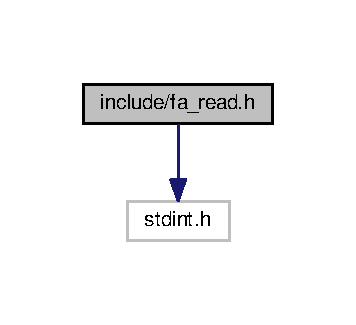
\includegraphics[width=181pt]{fa__read_8h__incl}
\end{center}
\end{figure}
This graph shows which files directly or indirectly include this file\+:
\nopagebreak
\begin{figure}[H]
\begin{center}
\leavevmode
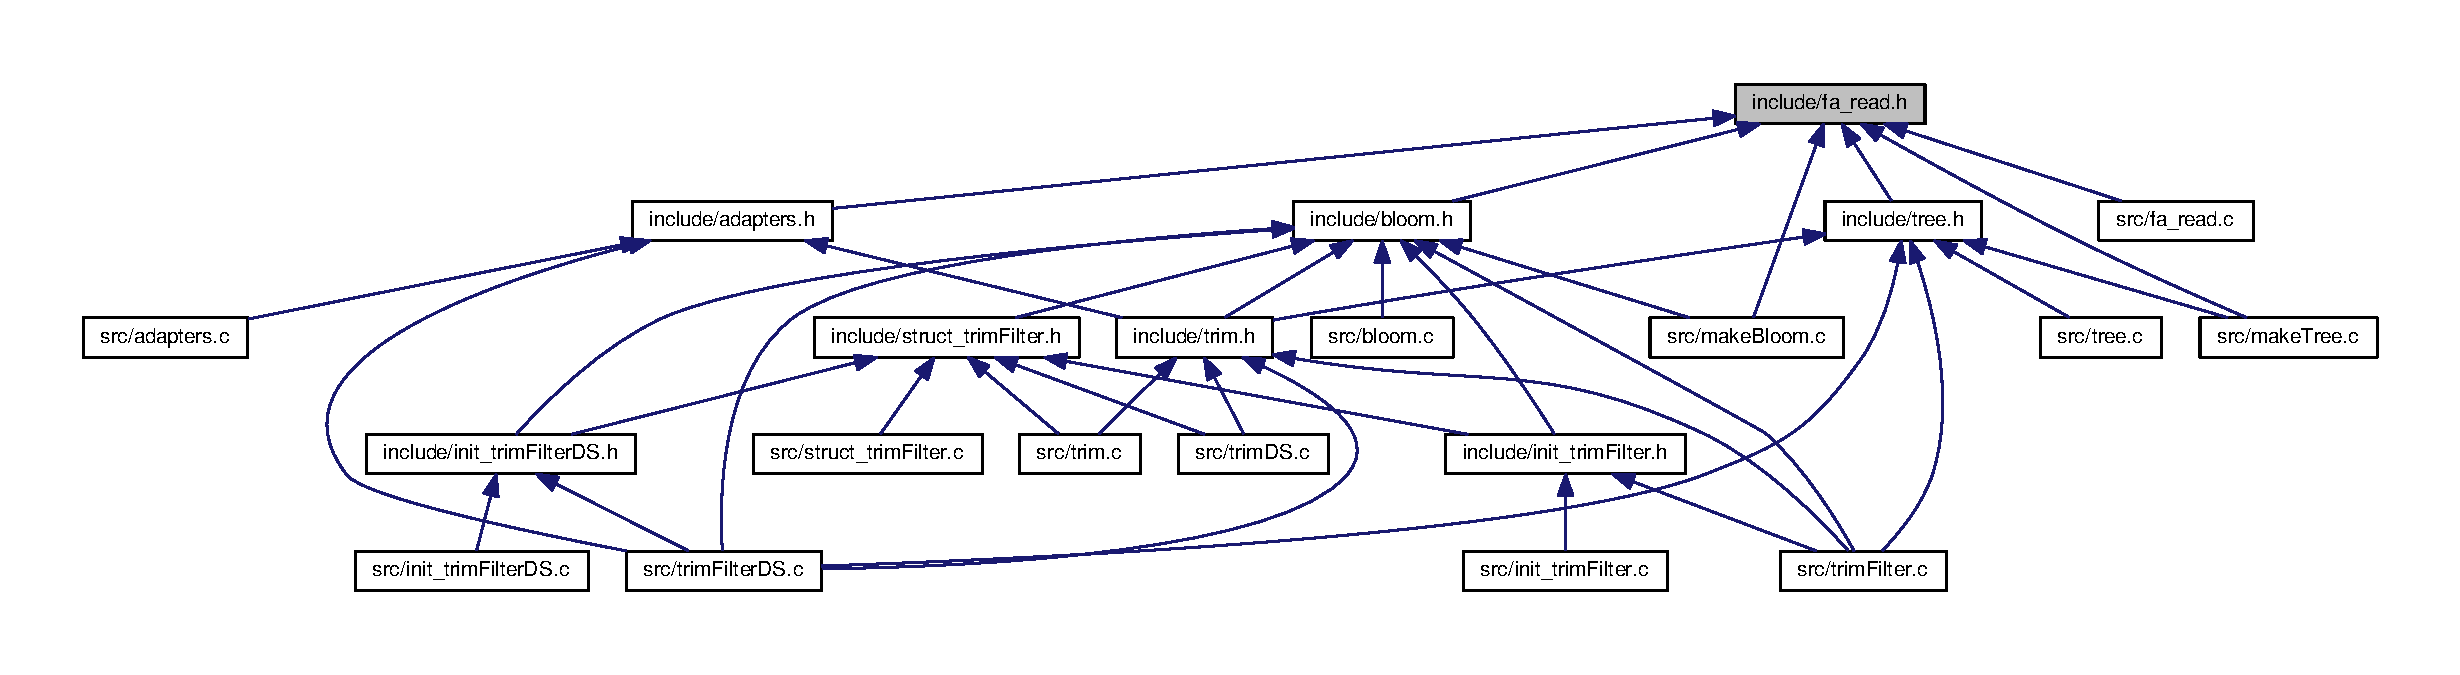
\includegraphics[width=350pt]{fa__read_8h__dep__incl}
\end{center}
\end{figure}
\subsection*{Classes}
\begin{DoxyCompactItemize}
\item 
struct \mbox{\hyperlink{struct__fa__entry}{\+\_\+fa\+\_\+entry}}
\begin{DoxyCompactList}\small\item\em fasta entry \end{DoxyCompactList}\item 
struct \mbox{\hyperlink{struct__fa__data}{\+\_\+fa\+\_\+data}}
\begin{DoxyCompactList}\small\item\em stores sequences of a fasta file \end{DoxyCompactList}\end{DoxyCompactItemize}
\subsection*{Typedefs}
\begin{DoxyCompactItemize}
\item 
\mbox{\Hypertarget{fa__read_8h_a8f68b28ad3a6c33fe1dd78d5ac044b30}\label{fa__read_8h_a8f68b28ad3a6c33fe1dd78d5ac044b30}} 
typedef struct \mbox{\hyperlink{struct__fa__entry}{\+\_\+fa\+\_\+entry}} \mbox{\hyperlink{fa__read_8h_a8f68b28ad3a6c33fe1dd78d5ac044b30}{Fa\+\_\+entry}}
\begin{DoxyCompactList}\small\item\em fasta entry \end{DoxyCompactList}\item 
\mbox{\Hypertarget{fa__read_8h_a797328b16bc1c1088998cd164aafb09d}\label{fa__read_8h_a797328b16bc1c1088998cd164aafb09d}} 
typedef struct \mbox{\hyperlink{struct__fa__data}{\+\_\+fa\+\_\+data}} \mbox{\hyperlink{fa__read_8h_a797328b16bc1c1088998cd164aafb09d}{Fa\+\_\+data}}
\begin{DoxyCompactList}\small\item\em stores sequences of a fasta file \end{DoxyCompactList}\end{DoxyCompactItemize}
\subsection*{Functions}
\begin{DoxyCompactItemize}
\item 
int \mbox{\hyperlink{fa__read_8h_a4d2d77d66924fdc762222c8f28f9718a}{read\+\_\+fasta}} (char $\ast$filename, \mbox{\hyperlink{fa__read_8h_a797328b16bc1c1088998cd164aafb09d}{Fa\+\_\+data}} $\ast$ptr\+\_\+fa)
\begin{DoxyCompactList}\small\item\em reads a fasta file and stores the contents in a Fa\+\_\+data structure. \end{DoxyCompactList}\item 
uint64\+\_\+t \mbox{\hyperlink{fa__read_8h_a0e6b9d47a8472d0768270afbdbf17d4e}{size\+\_\+fasta}} (\mbox{\hyperlink{fa__read_8h_a797328b16bc1c1088998cd164aafb09d}{Fa\+\_\+data}} $\ast$ptr\+\_\+fa)
\begin{DoxyCompactList}\small\item\em computes length of genome in fasta structure \end{DoxyCompactList}\item 
uint64\+\_\+t \mbox{\hyperlink{fa__read_8h_a73143a443a198eaf51820e5862f8547b}{nkmers}} (\mbox{\hyperlink{fa__read_8h_a797328b16bc1c1088998cd164aafb09d}{Fa\+\_\+data}} $\ast$ptr\+\_\+fa, int kmersize)
\begin{DoxyCompactList}\small\item\em number of kmers of length kmersize contained in a fasta structure \end{DoxyCompactList}\item 
void \mbox{\hyperlink{fa__read_8h_a714b70ff332a85349cd52b76965dd444}{free\+\_\+fasta}} (\mbox{\hyperlink{fa__read_8h_a797328b16bc1c1088998cd164aafb09d}{Fa\+\_\+data}} $\ast$ptr\+\_\+fa)
\begin{DoxyCompactList}\small\item\em free fasta file \end{DoxyCompactList}\end{DoxyCompactItemize}


\subsection{Detailed Description}
reads in and stores fasta files 

\begin{DoxyAuthor}{Author}
Paula Perez \href{mailto:paulaperezrubio@gmail.com}{\tt paulaperezrubio@gmail.\+com} 
\end{DoxyAuthor}
\begin{DoxyDate}{Date}
16.\+08.\+2017 
\end{DoxyDate}


\subsection{Function Documentation}
\mbox{\Hypertarget{fa__read_8h_a714b70ff332a85349cd52b76965dd444}\label{fa__read_8h_a714b70ff332a85349cd52b76965dd444}} 
\index{fa\+\_\+read.\+h@{fa\+\_\+read.\+h}!free\+\_\+fasta@{free\+\_\+fasta}}
\index{free\+\_\+fasta@{free\+\_\+fasta}!fa\+\_\+read.\+h@{fa\+\_\+read.\+h}}
\subsubsection{\texorpdfstring{free\+\_\+fasta()}{free\_fasta()}}
{\footnotesize\ttfamily void free\+\_\+fasta (\begin{DoxyParamCaption}\item[{\mbox{\hyperlink{fa__read_8h_a797328b16bc1c1088998cd164aafb09d}{Fa\+\_\+data}} $\ast$}]{ptr\+\_\+fa }\end{DoxyParamCaption})}



free fasta file 


\begin{DoxyParams}{Parameters}
{\em ptr\+\_\+fa} & pointer to Fa\+\_\+data structure.\\
\hline
\end{DoxyParams}
The dynamically allocated memory in a Fa\+\_\+data struct is deallocated and counted, so that we can \mbox{\Hypertarget{fa__read_8h_a73143a443a198eaf51820e5862f8547b}\label{fa__read_8h_a73143a443a198eaf51820e5862f8547b}} 
\index{fa\+\_\+read.\+h@{fa\+\_\+read.\+h}!nkmers@{nkmers}}
\index{nkmers@{nkmers}!fa\+\_\+read.\+h@{fa\+\_\+read.\+h}}
\subsubsection{\texorpdfstring{nkmers()}{nkmers()}}
{\footnotesize\ttfamily uint64\+\_\+t nkmers (\begin{DoxyParamCaption}\item[{\mbox{\hyperlink{fa__read_8h_a797328b16bc1c1088998cd164aafb09d}{Fa\+\_\+data}} $\ast$}]{ptr\+\_\+fa,  }\item[{int}]{kmersize }\end{DoxyParamCaption})}



number of kmers of length kmersize contained in a fasta structure 

\begin{DoxyReturn}{Returns}
number of kmers of length kmersize contained in a fasta structure 
\end{DoxyReturn}
\mbox{\Hypertarget{fa__read_8h_a4d2d77d66924fdc762222c8f28f9718a}\label{fa__read_8h_a4d2d77d66924fdc762222c8f28f9718a}} 
\index{fa\+\_\+read.\+h@{fa\+\_\+read.\+h}!read\+\_\+fasta@{read\+\_\+fasta}}
\index{read\+\_\+fasta@{read\+\_\+fasta}!fa\+\_\+read.\+h@{fa\+\_\+read.\+h}}
\subsubsection{\texorpdfstring{read\+\_\+fasta()}{read\_fasta()}}
{\footnotesize\ttfamily int read\+\_\+fasta (\begin{DoxyParamCaption}\item[{char $\ast$}]{filename,  }\item[{\mbox{\hyperlink{fa__read_8h_a797328b16bc1c1088998cd164aafb09d}{Fa\+\_\+data}} $\ast$}]{ptr\+\_\+fa }\end{DoxyParamCaption})}



reads a fasta file and stores the contents in a Fa\+\_\+data structure. 


\begin{DoxyParams}{Parameters}
{\em filename} & path to a fasta input file. \\
\hline
{\em ptr\+\_\+fa} & pointer to Fa\+\_\+data structure. \\
\hline
\end{DoxyParams}
\begin{DoxyReturn}{Returns}
number of entries in the fasta file.
\end{DoxyReturn}
A fasta file is read and stored in a structure Fa\+\_\+data The basic problem with reading F\+A\+S\+TA files is that there is no end-\/of-\/record indicator. When you\textquotesingle{}re reading sequence n, you don\textquotesingle{}t know you\textquotesingle{}re done until you\textquotesingle{}ve read the header line for sequence n+1, which you won\textquotesingle{}t parse \textquotesingle{}til later (when you\textquotesingle{}re reading in the sequence n+1). The solution implemented here is to read the file twice. The first time, (sweep\+\_\+fa), we initialize Fa\+\_\+data and store the parameters\+:
\begin{DoxyItemize}
\item nlines\+: number of lines of the fasta file.
\item nentries\+: number of entries in the fasta file.
\item linelen\+: length of a line in the considered fasta file.
\item entrylen\+: array containing the lengths of every entry. With this information, the pointer to Fa\+\_\+entry can be allocated and the file is read again and the entries are stored in the structure. 
\end{DoxyItemize}\mbox{\Hypertarget{fa__read_8h_a0e6b9d47a8472d0768270afbdbf17d4e}\label{fa__read_8h_a0e6b9d47a8472d0768270afbdbf17d4e}} 
\index{fa\+\_\+read.\+h@{fa\+\_\+read.\+h}!size\+\_\+fasta@{size\+\_\+fasta}}
\index{size\+\_\+fasta@{size\+\_\+fasta}!fa\+\_\+read.\+h@{fa\+\_\+read.\+h}}
\subsubsection{\texorpdfstring{size\+\_\+fasta()}{size\_fasta()}}
{\footnotesize\ttfamily uint64\+\_\+t size\+\_\+fasta (\begin{DoxyParamCaption}\item[{\mbox{\hyperlink{fa__read_8h_a797328b16bc1c1088998cd164aafb09d}{Fa\+\_\+data}} $\ast$}]{ptr\+\_\+fa }\end{DoxyParamCaption})}



computes length of genome in fasta structure 


\begin{DoxyParams}{Parameters}
{\em ptr\+\_\+fa} & pointer to Fa\+\_\+data \\
\hline
\end{DoxyParams}
\begin{DoxyReturn}{Returns}
total number of nucleotides 
\end{DoxyReturn}

\hypertarget{fopen__gen_8h}{\section{include/fopen\+\_\+gen.h File Reference}
\label{fopen__gen_8h}\index{include/fopen\+\_\+gen.\+h@{include/fopen\+\_\+gen.\+h}}
}


Uncompress/compress input/output files using pipes.  


{\ttfamily \#include $<$stdio.\+h$>$}\\*
Include dependency graph for fopen\+\_\+gen.\+h\+:\nopagebreak
\begin{figure}[H]
\begin{center}
\leavevmode
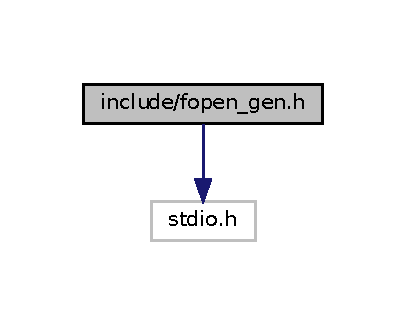
\includegraphics[width=184pt]{fopen__gen_8h__incl}
\end{center}
\end{figure}
This graph shows which files directly or indirectly include this file\+:\nopagebreak
\begin{figure}[H]
\begin{center}
\leavevmode
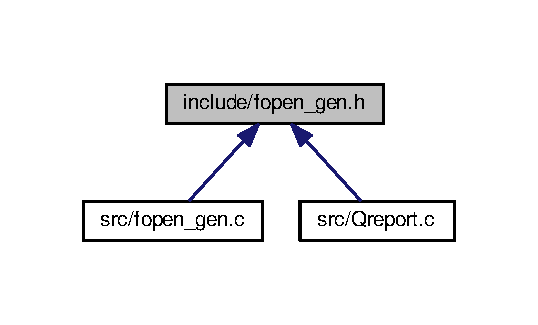
\includegraphics[width=258pt]{fopen__gen_8h__dep__incl}
\end{center}
\end{figure}
\subsection*{Macros}
\begin{DoxyCompactItemize}
\item 
\hypertarget{fopen__gen_8h_a2469c53816dc077f9deefb187ffcabf3}{\#define {\bfseries R\+E\+A\+D\+\_\+\+E\+N\+D}~0}\label{fopen__gen_8h_a2469c53816dc077f9deefb187ffcabf3}

\item 
\hypertarget{fopen__gen_8h_a2efd706d915e621e5e18b3f0803c4ed2}{\#define {\bfseries W\+R\+I\+T\+E\+\_\+\+E\+N\+D}~1}\label{fopen__gen_8h_a2efd706d915e621e5e18b3f0803c4ed2}

\item 
\hypertarget{fopen__gen_8h_a8b390f7305d3e2e82316936cde24101c}{\#define {\bfseries P\+E\+R\+M\+I\+S\+S\+I\+O\+N\+S}~0640}\label{fopen__gen_8h_a8b390f7305d3e2e82316936cde24101c}

\end{DoxyCompactItemize}
\subsection*{Functions}
\begin{DoxyCompactItemize}
\item 
\hypertarget{fopen__gen_8h_ae59755703d84f781f127762acf2deb6d}{int {\bfseries set\+Cloexec} (int fd)}\label{fopen__gen_8h_ae59755703d84f781f127762acf2deb6d}

\item 
F\+I\+L\+E $\ast$ \hyperlink{fopen__gen_8h_ae03fc1b9180f740dcb577fdb00072fb3}{fopen\+\_\+gen} (const char $\ast$path, const char $\ast$mode)
\begin{DoxyCompactList}\small\item\em Generalized fopen function. fopen\+\_\+gen is to be used as fopen. Can be used in read and in write mode. When used in read mode with a compressed extension, the file will be first decompressed and then read. When used in write mode with a compressed extension, the output will be compressed. \end{DoxyCompactList}\end{DoxyCompactItemize}


\subsection{Detailed Description}
Uncompress/compress input/output files using pipes. 

Hook the standard file opening functions, open, fopen and fopen64. If the extension of the file being opened indicates the file is compressed (.gz, .bz2, .xz), when opening in the reading mode a pipe to a program is opened that decompresses that file (gunzip, bunzip2 or xzdec) and return a handle to the open pipe. When opening in the writing mode (only for .gz, .bam), a pipe to a program is opened that compresses the output.

\begin{DoxyAuthor}{Author}
Paula Perez \href{mailto:paulaperezrubio@gmail.com}{\tt paulaperezrubio@gmail.\+com} 
\end{DoxyAuthor}
\begin{DoxyDate}{Date}
03.\+08.\+2017 
\end{DoxyDate}
\begin{DoxyWarning}{Warning}
vfork vs fork to be checked! 
\end{DoxyWarning}
\begin{DoxyNote}{Note}
-\/ original copyright note -\/ (reading mode, original C++ code) author\+: Shaun Jackman \href{mailto:sjackman@bcgsc.ca}{\tt sjackman@bcgsc.\+ca}, \href{https://github.com/bcgsc,}{\tt https\+://github.\+com/bcgsc,} filename\+: Uncompress.\+cpp 
\end{DoxyNote}


\subsection{Function Documentation}
\hypertarget{fopen__gen_8h_ae03fc1b9180f740dcb577fdb00072fb3}{\index{fopen\+\_\+gen.\+h@{fopen\+\_\+gen.\+h}!fopen\+\_\+gen@{fopen\+\_\+gen}}
\index{fopen\+\_\+gen@{fopen\+\_\+gen}!fopen\+\_\+gen.\+h@{fopen\+\_\+gen.\+h}}
\subsubsection[{fopen\+\_\+gen}]{\setlength{\rightskip}{0pt plus 5cm}F\+I\+L\+E$\ast$ fopen\+\_\+gen (
\begin{DoxyParamCaption}
\item[{const char $\ast$}]{path, }
\item[{const char $\ast$}]{mode}
\end{DoxyParamCaption}
)}}\label{fopen__gen_8h_ae03fc1b9180f740dcb577fdb00072fb3}


Generalized fopen function. fopen\+\_\+gen is to be used as fopen. Can be used in read and in write mode. When used in read mode with a compressed extension, the file will be first decompressed and then read. When used in write mode with a compressed extension, the output will be compressed. 

\begin{DoxyReturn}{Returns}
a F\+I\+L\+E pointer 
\end{DoxyReturn}

\hypertarget{fq__read_8h}{}\section{include/fq\+\_\+read.h File Reference}
\label{fq__read_8h}\index{include/fq\+\_\+read.\+h@{include/fq\+\_\+read.\+h}}


fastq entries manipulations (read/write)  


{\ttfamily \#include \char`\"{}config.\+h\char`\"{}}\newline
Include dependency graph for fq\+\_\+read.\+h\+:
\nopagebreak
\begin{figure}[H]
\begin{center}
\leavevmode
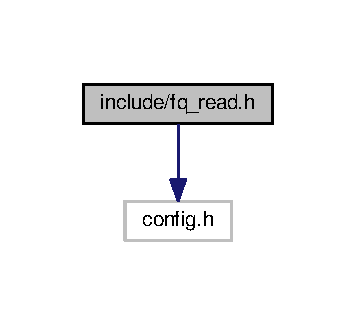
\includegraphics[width=181pt]{fq__read_8h__incl}
\end{center}
\end{figure}
This graph shows which files directly or indirectly include this file\+:
\nopagebreak
\begin{figure}[H]
\begin{center}
\leavevmode
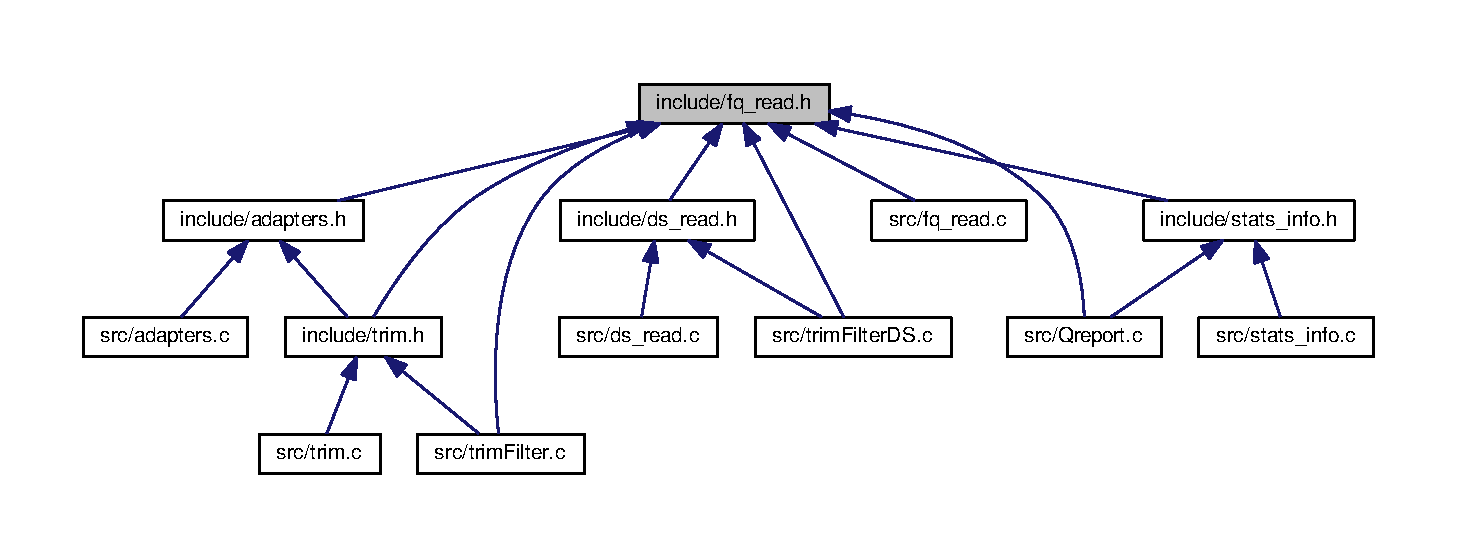
\includegraphics[width=350pt]{fq__read_8h__dep__incl}
\end{center}
\end{figure}
\subsection*{Classes}
\begin{DoxyCompactItemize}
\item 
struct \mbox{\hyperlink{struct__fq__read}{\+\_\+fq\+\_\+read}}
\begin{DoxyCompactList}\small\item\em stores a fastq entry \end{DoxyCompactList}\end{DoxyCompactItemize}
\subsection*{Typedefs}
\begin{DoxyCompactItemize}
\item 
\mbox{\Hypertarget{fq__read_8h_a9af37aa81397c9531c66863d4e97f034}\label{fq__read_8h_a9af37aa81397c9531c66863d4e97f034}} 
typedef struct \mbox{\hyperlink{struct__fq__read}{\+\_\+fq\+\_\+read}} \mbox{\hyperlink{fq__read_8h_a9af37aa81397c9531c66863d4e97f034}{Fq\+\_\+read}}
\begin{DoxyCompactList}\small\item\em stores a fastq entry \end{DoxyCompactList}\end{DoxyCompactItemize}
\subsection*{Functions}
\begin{DoxyCompactItemize}
\item 
int \mbox{\hyperlink{fq__read_8h_af0d30098d51bea3d11c442c3dd60e15f}{get\+\_\+fqread}} (\mbox{\hyperlink{fq__read_8h_a9af37aa81397c9531c66863d4e97f034}{Fq\+\_\+read}} $\ast$seq, char $\ast$buffer, int pos1, int pos2, int nline, int read\+\_\+len, int filter)
\begin{DoxyCompactList}\small\item\em reads fastq line from a buffer \end{DoxyCompactList}\item 
int \mbox{\hyperlink{fq__read_8h_ae58e185777143cd1fc4c75fccd5c647a}{string\+\_\+seq}} (\mbox{\hyperlink{fq__read_8h_a9af37aa81397c9531c66863d4e97f034}{Fq\+\_\+read}} $\ast$seq, char $\ast$char\+\_\+seq)
\begin{DoxyCompactList}\small\item\em writes the fq entry in a string \end{DoxyCompactList}\end{DoxyCompactItemize}


\subsection{Detailed Description}
fastq entries manipulations (read/write) 

\begin{DoxyAuthor}{Author}
Paula Perez \href{mailto:paulaperezrubio@gmail.com}{\tt paulaperezrubio@gmail.\+com} 
\end{DoxyAuthor}
\begin{DoxyDate}{Date}
03.\+08.\+2017 
\end{DoxyDate}


\subsection{Function Documentation}
\mbox{\Hypertarget{fq__read_8h_af0d30098d51bea3d11c442c3dd60e15f}\label{fq__read_8h_af0d30098d51bea3d11c442c3dd60e15f}} 
\index{fq\+\_\+read.\+h@{fq\+\_\+read.\+h}!get\+\_\+fqread@{get\+\_\+fqread}}
\index{get\+\_\+fqread@{get\+\_\+fqread}!fq\+\_\+read.\+h@{fq\+\_\+read.\+h}}
\subsubsection{\texorpdfstring{get\+\_\+fqread()}{get\_fqread()}}
{\footnotesize\ttfamily int get\+\_\+fqread (\begin{DoxyParamCaption}\item[{\mbox{\hyperlink{fq__read_8h_a9af37aa81397c9531c66863d4e97f034}{Fq\+\_\+read}} $\ast$}]{seq,  }\item[{char $\ast$}]{buffer,  }\item[{int}]{pos1,  }\item[{int}]{pos2,  }\item[{int}]{nline,  }\item[{int}]{read\+\_\+len,  }\item[{int}]{filter }\end{DoxyParamCaption})}



reads fastq line from a buffer 

a fastq line is read from a buffer and the relevant information is stored in a structure {\bfseries Fq\+\_\+read}. Depending on the value of {\bfseries filter}, information about whether the read was trimmed is stored.


\begin{DoxyParams}{Parameters}
{\em seq} & pointer to {\bfseries Fq\+\_\+read}, where the info will be stored. \\
\hline
{\em buffer} & variable where the file being read is stored. \\
\hline
{\em pos1} & buffer start position of the line. \\
\hline
{\em pos2} & buffer end position of the line. \\
\hline
{\em nline} & file line number being read. \\
\hline
{\em read\+\_\+len} & predefined read length \\
\hline
{\em filter} & 0 original file, 1 file filtered with filter\+\_\+trim, 2 file filtered with another tool \\
\hline
\end{DoxyParams}
\mbox{\Hypertarget{fq__read_8h_ae58e185777143cd1fc4c75fccd5c647a}\label{fq__read_8h_ae58e185777143cd1fc4c75fccd5c647a}} 
\index{fq\+\_\+read.\+h@{fq\+\_\+read.\+h}!string\+\_\+seq@{string\+\_\+seq}}
\index{string\+\_\+seq@{string\+\_\+seq}!fq\+\_\+read.\+h@{fq\+\_\+read.\+h}}
\subsubsection{\texorpdfstring{string\+\_\+seq()}{string\_seq()}}
{\footnotesize\ttfamily int string\+\_\+seq (\begin{DoxyParamCaption}\item[{\mbox{\hyperlink{fq__read_8h_a9af37aa81397c9531c66863d4e97f034}{Fq\+\_\+read}} $\ast$}]{seq,  }\item[{char $\ast$}]{char\+\_\+seq }\end{DoxyParamCaption})}



writes the fq entry in a string 


\begin{DoxyParams}{Parameters}
{\em seq} & pointer to {\bfseries Fq\+\_\+read}, where the info will be stored. \\
\hline
{\em char\+\_\+seq} & pointer to buffer, where the sequence will be stored \\
\hline
\end{DoxyParams}
\begin{DoxyWarning}{Warning}
change the call to sprintf to snprintf 
\end{DoxyWarning}

\hypertarget{init__Freport_8h}{\section{include/init\+\_\+\+Freport.h File Reference}
\label{init__Freport_8h}\index{include/init\+\_\+\+Freport.\+h@{include/init\+\_\+\+Freport.\+h}}
}


Help dialog for Freport and initialization of the command line arguments.  


{\ttfamily \#include \char`\"{}defines.\+h\char`\"{}}\\*
Include dependency graph for init\+\_\+\+Freport.\+h\+:\nopagebreak
\begin{figure}[H]
\begin{center}
\leavevmode
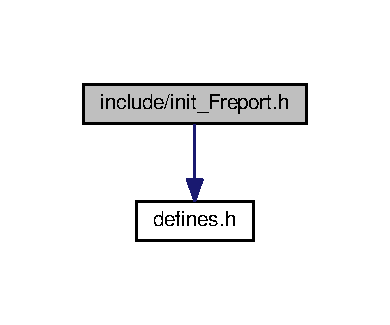
\includegraphics[width=187pt]{init__Freport_8h__incl}
\end{center}
\end{figure}
This graph shows which files directly or indirectly include this file\+:\nopagebreak
\begin{figure}[H]
\begin{center}
\leavevmode
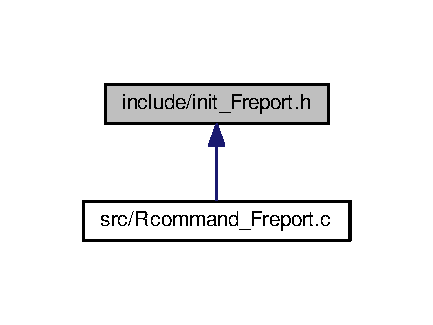
\includegraphics[width=208pt]{init__Freport_8h__dep__incl}
\end{center}
\end{figure}
\subsection*{Classes}
\begin{DoxyCompactItemize}
\item 
struct \hyperlink{struct__iparam__Freport}{\+\_\+iparam\+\_\+\+Freport}
\begin{DoxyCompactList}\small\item\em contains Freport input parameters \end{DoxyCompactList}\end{DoxyCompactItemize}
\subsection*{Typedefs}
\begin{DoxyCompactItemize}
\item 
\hypertarget{init__Freport_8h_ad8a9800538d457840314d0c39b15c0db}{typedef struct \hyperlink{struct__iparam__Freport}{\+\_\+iparam\+\_\+\+Freport} \hyperlink{init__Freport_8h_ad8a9800538d457840314d0c39b15c0db}{Iparam\+\_\+\+Freport}}\label{init__Freport_8h_ad8a9800538d457840314d0c39b15c0db}

\begin{DoxyCompactList}\small\item\em contains Freport input parameters \end{DoxyCompactList}\end{DoxyCompactItemize}
\subsection*{Functions}
\begin{DoxyCompactItemize}
\item 
\hypertarget{init__Freport_8h_adab6eff75b2f4a454778e8b8e4a786e3}{void {\bfseries print\+Help\+Dialog\+\_\+\+Freport} ()}\label{init__Freport_8h_adab6eff75b2f4a454778e8b8e4a786e3}

\item 
\hypertarget{init__Freport_8h_a5304e51a735167d036d9b34fcf0430af}{void {\bfseries getarg\+\_\+\+Freport} (int argc, char $\ast$$\ast$argv)}\label{init__Freport_8h_a5304e51a735167d036d9b34fcf0430af}

\end{DoxyCompactItemize}


\subsection{Detailed Description}
Help dialog for Freport and initialization of the command line arguments. 

\begin{DoxyAuthor}{Author}
Paula Perez \href{mailto:paulaperezrubio@gmail.com}{\tt paulaperezrubio@gmail.\+com} 
\end{DoxyAuthor}
\begin{DoxyDate}{Date}
01.\+09.\+2017 
\end{DoxyDate}

\hypertarget{init__makeTree_8h}{}\section{include/init\+\_\+make\+Tree.h File Reference}
\label{init__makeTree_8h}\index{include/init\+\_\+make\+Tree.\+h@{include/init\+\_\+make\+Tree.\+h}}


Help dialog for make\+Tree and initialization of the command line arguments.  


{\ttfamily \#include \char`\"{}defines.\+h\char`\"{}}\newline
Include dependency graph for init\+\_\+make\+Tree.\+h\+:
\nopagebreak
\begin{figure}[H]
\begin{center}
\leavevmode
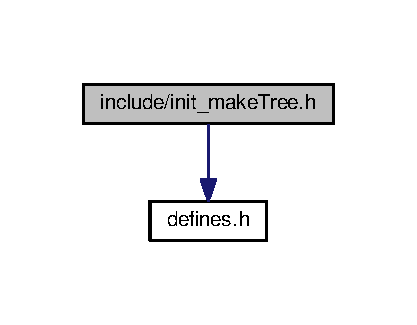
\includegraphics[width=218pt]{init__makeTree_8h__incl}
\end{center}
\end{figure}
This graph shows which files directly or indirectly include this file\+:
\nopagebreak
\begin{figure}[H]
\begin{center}
\leavevmode
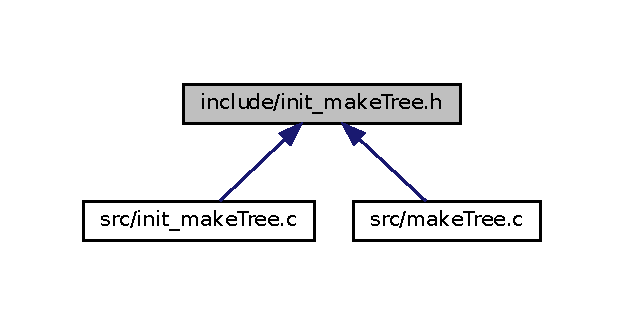
\includegraphics[width=300pt]{init__makeTree_8h__dep__incl}
\end{center}
\end{figure}
\subsection*{Classes}
\begin{DoxyCompactItemize}
\item 
struct \mbox{\hyperlink{struct__iparam__makeTree}{\+\_\+iparam\+\_\+make\+Tree}}
\begin{DoxyCompactList}\small\item\em contains make\+Tree input parameters \end{DoxyCompactList}\end{DoxyCompactItemize}
\subsection*{Typedefs}
\begin{DoxyCompactItemize}
\item 
\mbox{\Hypertarget{init__makeTree_8h_a10d824f48589000a94c210c64f08c9a9}\label{init__makeTree_8h_a10d824f48589000a94c210c64f08c9a9}} 
typedef struct \mbox{\hyperlink{struct__iparam__makeTree}{\+\_\+iparam\+\_\+make\+Tree}} \mbox{\hyperlink{init__makeTree_8h_a10d824f48589000a94c210c64f08c9a9}{Iparam\+\_\+make\+Tree}}
\begin{DoxyCompactList}\small\item\em contains make\+Tree input parameters \end{DoxyCompactList}\end{DoxyCompactItemize}
\subsection*{Functions}
\begin{DoxyCompactItemize}
\item 
\mbox{\Hypertarget{init__makeTree_8h_a51fb8fb2c64bc9dca004b0e0ecb3997a}\label{init__makeTree_8h_a51fb8fb2c64bc9dca004b0e0ecb3997a}} 
void \mbox{\hyperlink{init__makeTree_8h_a51fb8fb2c64bc9dca004b0e0ecb3997a}{print\+Help\+Dialog\+\_\+make\+Tree}} ()
\begin{DoxyCompactList}\small\item\em Function that prints make\+Tree help dialog when called. \end{DoxyCompactList}\item 
\mbox{\Hypertarget{init__makeTree_8h_a175c3eda9f2120856c04f9bbf4b1bdad}\label{init__makeTree_8h_a175c3eda9f2120856c04f9bbf4b1bdad}} 
void \mbox{\hyperlink{init__makeTree_8h_a175c3eda9f2120856c04f9bbf4b1bdad}{getarg\+\_\+make\+Tree}} (int argc, char $\ast$$\ast$argv)
\begin{DoxyCompactList}\small\item\em Reads in the arguments passed through the command line to make\+Tree. and stores them in the global variable par\+\_\+\+MT. \end{DoxyCompactList}\end{DoxyCompactItemize}


\subsection{Detailed Description}
Help dialog for make\+Tree and initialization of the command line arguments. 

\begin{DoxyAuthor}{Author}
Paula Perez \href{mailto:paulaperezrubio@gmail.com}{\tt paulaperezrubio@gmail.\+com} 
\end{DoxyAuthor}
\begin{DoxyDate}{Date}
23.\+08.\+2017 
\end{DoxyDate}

\hypertarget{init__Qreport_8h}{}\section{include/init\+\_\+\+Qreport.h File Reference}
\label{init__Qreport_8h}\index{include/init\+\_\+\+Qreport.\+h@{include/init\+\_\+\+Qreport.\+h}}


Header file\+: help dialog for Qreport and initialization of the command line arguments.  


{\ttfamily \#include \char`\"{}defines.\+h\char`\"{}}\newline
Include dependency graph for init\+\_\+\+Qreport.\+h\+:
\nopagebreak
\begin{figure}[H]
\begin{center}
\leavevmode
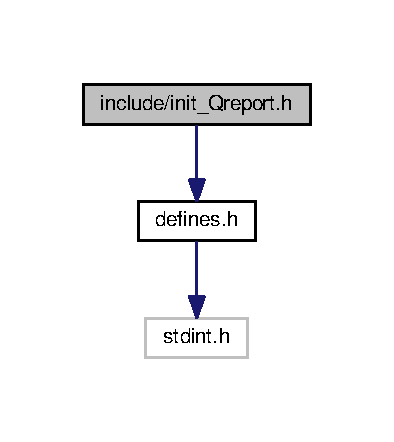
\includegraphics[width=216pt]{init__Qreport_8h__incl}
\end{center}
\end{figure}
This graph shows which files directly or indirectly include this file\+:
\nopagebreak
\begin{figure}[H]
\begin{center}
\leavevmode
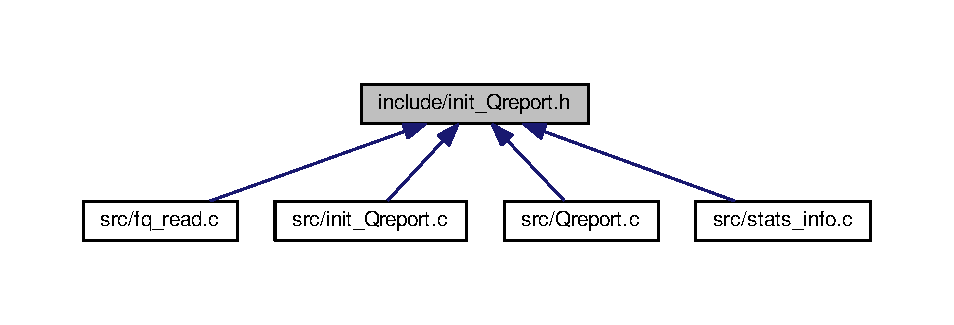
\includegraphics[width=350pt]{init__Qreport_8h__dep__incl}
\end{center}
\end{figure}
\subsection*{Classes}
\begin{DoxyCompactItemize}
\item 
struct \mbox{\hyperlink{struct__iparam__Qreport}{\+\_\+iparam\+\_\+\+Qreport}}
\begin{DoxyCompactList}\small\item\em contains Qreport input parameters \end{DoxyCompactList}\end{DoxyCompactItemize}
\subsection*{Typedefs}
\begin{DoxyCompactItemize}
\item 
\mbox{\Hypertarget{init__Qreport_8h_a883b1b3db368b84ab55f011bbb41bc80}\label{init__Qreport_8h_a883b1b3db368b84ab55f011bbb41bc80}} 
typedef struct \mbox{\hyperlink{struct__iparam__Qreport}{\+\_\+iparam\+\_\+\+Qreport}} \mbox{\hyperlink{init__Qreport_8h_a883b1b3db368b84ab55f011bbb41bc80}{Iparam\+\_\+\+Qreport}}
\begin{DoxyCompactList}\small\item\em contains Qreport input parameters \end{DoxyCompactList}\end{DoxyCompactItemize}
\subsection*{Functions}
\begin{DoxyCompactItemize}
\item 
\mbox{\Hypertarget{init__Qreport_8h_a48be775a109c8bf8672933494d67f30f}\label{init__Qreport_8h_a48be775a109c8bf8672933494d67f30f}} 
void \mbox{\hyperlink{init__Qreport_8h_a48be775a109c8bf8672933494d67f30f}{print\+Help\+Dialog\+\_\+\+Qreport}} ()
\begin{DoxyCompactList}\small\item\em Function that prints Qreport help dialog when called. \end{DoxyCompactList}\item 
\mbox{\Hypertarget{init__Qreport_8h_a0eb2d9339158f29ffe7ae419af56e921}\label{init__Qreport_8h_a0eb2d9339158f29ffe7ae419af56e921}} 
void \mbox{\hyperlink{init__Qreport_8h_a0eb2d9339158f29ffe7ae419af56e921}{getarg\+\_\+\+Qreport}} (int argc, char $\ast$$\ast$argv)
\begin{DoxyCompactList}\small\item\em Reads in the arguments passed through the command line to Qreport. and stores them in the global variable par\+\_\+\+QR. \end{DoxyCompactList}\end{DoxyCompactItemize}


\subsection{Detailed Description}
Header file\+: help dialog for Qreport and initialization of the command line arguments. 

\begin{DoxyAuthor}{Author}
Paula Perez \href{mailto:paulaperezrubio@gmail.com}{\tt paulaperezrubio@gmail.\+com} 
\end{DoxyAuthor}
\begin{DoxyDate}{Date}
03.\+08.\+2017 
\end{DoxyDate}

\hypertarget{init__Sreport_8h}{}\section{include/init\+\_\+\+Sreport.h File Reference}
\label{init__Sreport_8h}\index{include/init\+\_\+\+Sreport.\+h@{include/init\+\_\+\+Sreport.\+h}}


Help dialog for Sreport and initialization of the command line arguments.  


{\ttfamily \#include \char`\"{}defines.\+h\char`\"{}}\newline
Include dependency graph for init\+\_\+\+Sreport.\+h\+:
\nopagebreak
\begin{figure}[H]
\begin{center}
\leavevmode
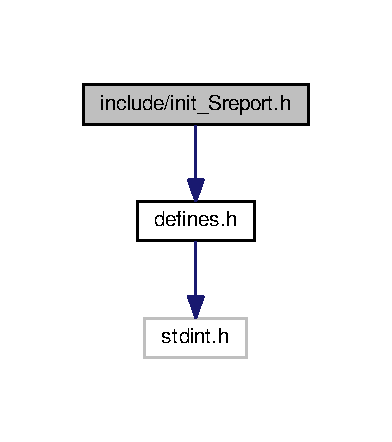
\includegraphics[width=216pt]{init__Sreport_8h__incl}
\end{center}
\end{figure}
This graph shows which files directly or indirectly include this file\+:
\nopagebreak
\begin{figure}[H]
\begin{center}
\leavevmode
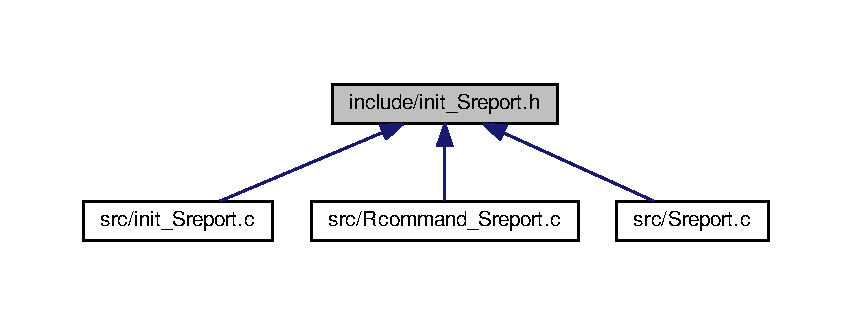
\includegraphics[width=350pt]{init__Sreport_8h__dep__incl}
\end{center}
\end{figure}
\subsection*{Classes}
\begin{DoxyCompactItemize}
\item 
struct \mbox{\hyperlink{struct__iparam__Sreport}{\+\_\+iparam\+\_\+\+Sreport}}
\begin{DoxyCompactList}\small\item\em contains Sreport input parameters \end{DoxyCompactList}\end{DoxyCompactItemize}
\subsection*{Typedefs}
\begin{DoxyCompactItemize}
\item 
\mbox{\Hypertarget{init__Sreport_8h_ae7c35fd710a54db5b21f5c6b04fe9a5d}\label{init__Sreport_8h_ae7c35fd710a54db5b21f5c6b04fe9a5d}} 
typedef struct \mbox{\hyperlink{struct__iparam__Sreport}{\+\_\+iparam\+\_\+\+Sreport}} \mbox{\hyperlink{init__Sreport_8h_ae7c35fd710a54db5b21f5c6b04fe9a5d}{Iparam\+\_\+\+Sreport}}
\begin{DoxyCompactList}\small\item\em contains Sreport input parameters \end{DoxyCompactList}\end{DoxyCompactItemize}
\subsection*{Functions}
\begin{DoxyCompactItemize}
\item 
\mbox{\Hypertarget{init__Sreport_8h_a80638b0730feac5c7634c29c6f08ee9e}\label{init__Sreport_8h_a80638b0730feac5c7634c29c6f08ee9e}} 
void \mbox{\hyperlink{init__Sreport_8h_a80638b0730feac5c7634c29c6f08ee9e}{print\+Help\+Dialog\+\_\+\+Sreport}} ()
\begin{DoxyCompactList}\small\item\em Function that prints Sreport help dialog when called. \end{DoxyCompactList}\item 
\mbox{\Hypertarget{init__Sreport_8h_a5a266a01d36227a9094c023aed7a1e8c}\label{init__Sreport_8h_a5a266a01d36227a9094c023aed7a1e8c}} 
void \mbox{\hyperlink{init__Sreport_8h_a5a266a01d36227a9094c023aed7a1e8c}{getarg\+\_\+\+Sreport}} (int argc, char $\ast$$\ast$argv)
\begin{DoxyCompactList}\small\item\em Reads in the arguments passed through the command line to Sreport. and stores them in the global variable par\+\_\+\+SR. \end{DoxyCompactList}\end{DoxyCompactItemize}


\subsection{Detailed Description}
Help dialog for Sreport and initialization of the command line arguments. 

\begin{DoxyAuthor}{Author}
Paula Perez \href{mailto:paulaperezrubio@gmail.com}{\tt paulaperezrubio@gmail.\+com} 
\end{DoxyAuthor}
\begin{DoxyDate}{Date}
09.\+08.\+2017 
\end{DoxyDate}

\hypertarget{init__trimFilter_8h}{\section{include/init\+\_\+trim\+Filter.h File Reference}
\label{init__trimFilter_8h}\index{include/init\+\_\+trim\+Filter.\+h@{include/init\+\_\+trim\+Filter.\+h}}
}


help dialog for trim\+Filter and initialization of the command line arguments.  


{\ttfamily \#include \char`\"{}defines.\+h\char`\"{}}\\*
Include dependency graph for init\+\_\+trim\+Filter.\+h\+:\nopagebreak
\begin{figure}[H]
\begin{center}
\leavevmode
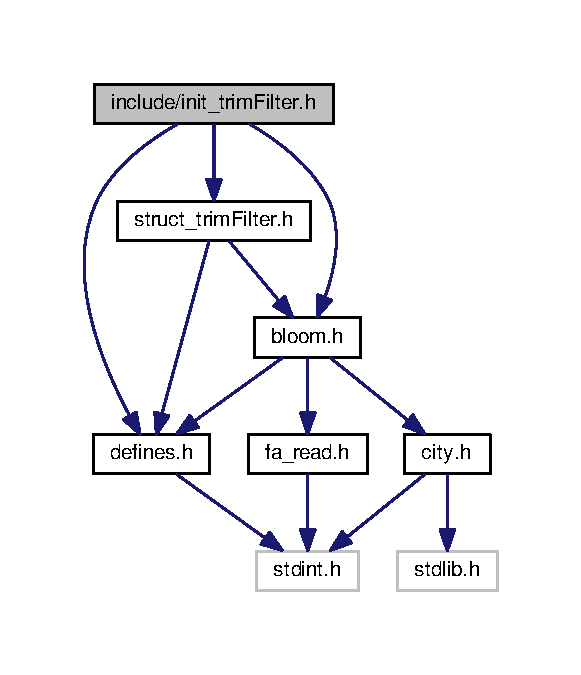
\includegraphics[width=195pt]{init__trimFilter_8h__incl}
\end{center}
\end{figure}
This graph shows which files directly or indirectly include this file\+:\nopagebreak
\begin{figure}[H]
\begin{center}
\leavevmode
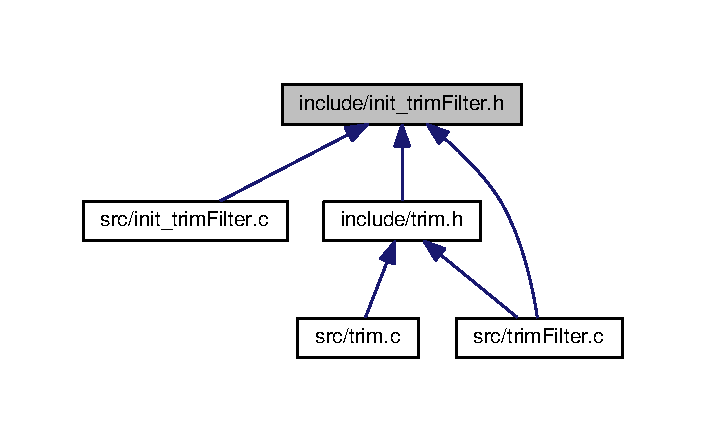
\includegraphics[width=339pt]{init__trimFilter_8h__dep__incl}
\end{center}
\end{figure}
\subsection*{Classes}
\begin{DoxyCompactItemize}
\item 
struct \hyperlink{struct__adapter}{\+\_\+adapter}
\item 
struct \hyperlink{struct__iparam__trimFilter}{\+\_\+iparam\+\_\+trim\+Filter}
\begin{DoxyCompactList}\small\item\em trim\+Filter input parameters \end{DoxyCompactList}\end{DoxyCompactItemize}
\subsection*{Typedefs}
\begin{DoxyCompactItemize}
\item 
typedef struct \hyperlink{struct__adapter}{\+\_\+adapter} \hyperlink{init__trimFilter_8h_a3442d07a10a4ab75064687f3c244e370}{Adapter}
\item 
\hypertarget{init__trimFilter_8h_aff83806f1ff2b5f3609dc7d4c04b7c19}{typedef struct \hyperlink{struct__iparam__trimFilter}{\+\_\+iparam\+\_\+trim\+Filter} \hyperlink{init__trimFilter_8h_aff83806f1ff2b5f3609dc7d4c04b7c19}{Iparam\+\_\+trim\+Filter}}\label{init__trimFilter_8h_aff83806f1ff2b5f3609dc7d4c04b7c19}

\begin{DoxyCompactList}\small\item\em trim\+Filter input parameters \end{DoxyCompactList}\end{DoxyCompactItemize}
\subsection*{Functions}
\begin{DoxyCompactItemize}
\item 
\hypertarget{init__trimFilter_8h_acb1b66de50f5bfccd87b52851f8de3cc}{void \hyperlink{init__trimFilter_8h_acb1b66de50f5bfccd87b52851f8de3cc}{print\+Help\+Dialog\+\_\+trim\+Filter} ()}\label{init__trimFilter_8h_acb1b66de50f5bfccd87b52851f8de3cc}

\begin{DoxyCompactList}\small\item\em Function that prints trim\+Filter help dialog when called. \end{DoxyCompactList}\item 
\hypertarget{init__trimFilter_8h_a4e5dbdc70417040f72231b5167987b4a}{void \hyperlink{init__trimFilter_8h_a4e5dbdc70417040f72231b5167987b4a}{getarg\+\_\+trim\+Filter} (int argc, char $\ast$$\ast$argv)}\label{init__trimFilter_8h_a4e5dbdc70417040f72231b5167987b4a}

\begin{DoxyCompactList}\small\item\em Reads in the arguments passed through the command line to trim\+Filter. and stores them in the global variable par\+\_\+\+T\+F. \end{DoxyCompactList}\end{DoxyCompactItemize}


\subsection{Detailed Description}
help dialog for trim\+Filter and initialization of the command line arguments. 

\begin{DoxyAuthor}{Author}
Paula Perez \href{mailto:paulaperezrubio@gmail.com}{\tt paulaperezrubio@gmail.\+com} 
\end{DoxyAuthor}
\begin{DoxyDate}{Date}
24.\+08.\+2017 
\end{DoxyDate}


\subsection{Typedef Documentation}
\hypertarget{init__trimFilter_8h_a3442d07a10a4ab75064687f3c244e370}{\index{init\+\_\+trim\+Filter.\+h@{init\+\_\+trim\+Filter.\+h}!Adapter@{Adapter}}
\index{Adapter@{Adapter}!init\+\_\+trim\+Filter.\+h@{init\+\_\+trim\+Filter.\+h}}
\subsubsection[{Adapter}]{\setlength{\rightskip}{0pt plus 5cm}typedef struct {\bf \+\_\+adapter}  {\bf Adapter}}}\label{init__trimFilter_8h_a3442d07a10a4ab75064687f3c244e370}
@ brief adapter struct @ note U\+N\+F\+I\+N\+I\+S\+H\+E\+D! 
\hypertarget{io__trimFilter_8h}{\section{include/io\+\_\+trim\+Filter.h File Reference}
\label{io__trimFilter_8h}\index{include/io\+\_\+trim\+Filter.\+h@{include/io\+\_\+trim\+Filter.\+h}}
}


buffer fq output, write summary file  


{\ttfamily \#include $<$stdio.\+h$>$}\\*
{\ttfamily \#include \char`\"{}defines.\+h\char`\"{}}\\*
Include dependency graph for io\+\_\+trim\+Filter.\+h\+:\nopagebreak
\begin{figure}[H]
\begin{center}
\leavevmode
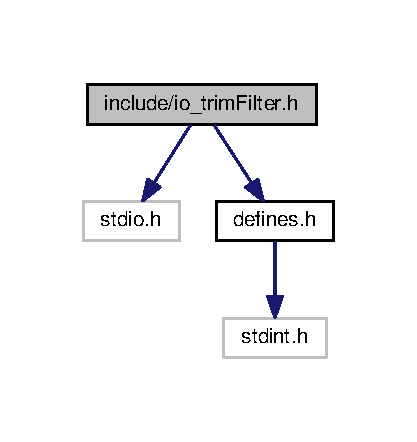
\includegraphics[width=200pt]{io__trimFilter_8h__incl}
\end{center}
\end{figure}
This graph shows which files directly or indirectly include this file\+:\nopagebreak
\begin{figure}[H]
\begin{center}
\leavevmode
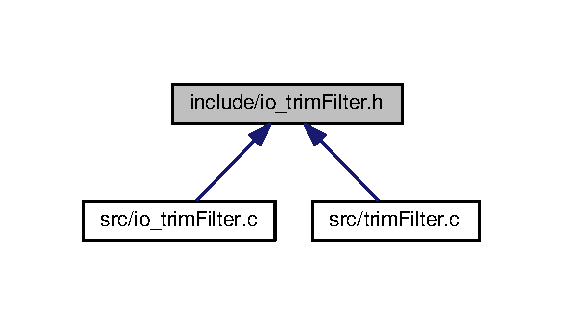
\includegraphics[width=270pt]{io__trimFilter_8h__dep__incl}
\end{center}
\end{figure}
\subsection*{Classes}
\begin{DoxyCompactItemize}
\item 
struct \hyperlink{struct__stats__TF}{\+\_\+stats\+\_\+\+T\+F}
\begin{DoxyCompactList}\small\item\em collects stats info from the filtering procedure \end{DoxyCompactList}\end{DoxyCompactItemize}
\subsection*{Typedefs}
\begin{DoxyCompactItemize}
\item 
\hypertarget{io__trimFilter_8h_a9b921e335cd93e3ad72901eca22b7758}{typedef struct \hyperlink{struct__stats__TF}{\+\_\+stats\+\_\+\+T\+F} \hyperlink{io__trimFilter_8h_a9b921e335cd93e3ad72901eca22b7758}{Stats\+\_\+\+T\+F}}\label{io__trimFilter_8h_a9b921e335cd93e3ad72901eca22b7758}

\begin{DoxyCompactList}\small\item\em collects stats info from the filtering procedure \end{DoxyCompactList}\end{DoxyCompactItemize}
\subsection*{Functions}
\begin{DoxyCompactItemize}
\item 
void \hyperlink{io__trimFilter_8h_aded957d5c9c0bb7e6479a578c949c7ac}{buffer\+\_\+output} (F\+I\+L\+E $\ast$fout, const char $\ast$a, const int len, const int fd\+\_\+i)
\begin{DoxyCompactList}\small\item\em buffers the output before writing to disk, writes out summary \end{DoxyCompactList}\item 
\hypertarget{io__trimFilter_8h_a4091d7483c30847a4bea4dabe00c4ffb}{void \hyperlink{io__trimFilter_8h_a4091d7483c30847a4bea4dabe00c4ffb}{write\+\_\+summary\+\_\+\+T\+F} (\hyperlink{io__trimFilter_8h_a9b921e335cd93e3ad72901eca22b7758}{Stats\+\_\+\+T\+F} tf\+\_\+stats, char $\ast$filename)}\label{io__trimFilter_8h_a4091d7483c30847a4bea4dabe00c4ffb}

\begin{DoxyCompactList}\small\item\em writes stats of filtering to summary file (binary) \end{DoxyCompactList}\end{DoxyCompactItemize}


\subsection{Detailed Description}
buffer fq output, write summary file 

\begin{DoxyAuthor}{Author}
Paula Perez \href{mailto:paulaperezrubio@gmail.com}{\tt paulaperezrubio@gmail.\+com} 
\end{DoxyAuthor}
\begin{DoxyDate}{Date}
29.\+08.\+2017 
\end{DoxyDate}


\subsection{Function Documentation}
\hypertarget{io__trimFilter_8h_aded957d5c9c0bb7e6479a578c949c7ac}{\index{io\+\_\+trim\+Filter.\+h@{io\+\_\+trim\+Filter.\+h}!buffer\+\_\+output@{buffer\+\_\+output}}
\index{buffer\+\_\+output@{buffer\+\_\+output}!io\+\_\+trim\+Filter.\+h@{io\+\_\+trim\+Filter.\+h}}
\subsubsection[{buffer\+\_\+output}]{\setlength{\rightskip}{0pt plus 5cm}void buffer\+\_\+output (
\begin{DoxyParamCaption}
\item[{F\+I\+L\+E $\ast$}]{fout, }
\item[{const char $\ast$}]{str, }
\item[{const int}]{len, }
\item[{const int}]{fd\+\_\+i}
\end{DoxyParamCaption}
)}}\label{io__trimFilter_8h_aded957d5c9c0bb7e6479a578c949c7ac}


buffers the output before writing to disk, writes out summary 


\begin{DoxyParams}{Parameters}
{\em fout} & F\+I\+L\+E pointer where we might write to disk; \\
\hline
{\em str} & string we want to add \\
\hline
{\em len} & length of the string we want to add \\
\hline
{\em fd\+\_\+i} & identifier\+: G\+O\+O\+D, A\+D\+A\+P, C\+O\+N\+T, L\+O\+W\+Q, N\+N\+N\+N \\
\hline
\end{DoxyParams}

\hypertarget{Lmer_8h}{\section{include/\+Lmer.h File Reference}
\label{Lmer_8h}\index{include/\+Lmer.\+h@{include/\+Lmer.\+h}}
}


Manipulation of Lmers and sequences.  


This graph shows which files directly or indirectly include this file\+:\nopagebreak
\begin{figure}[H]
\begin{center}
\leavevmode
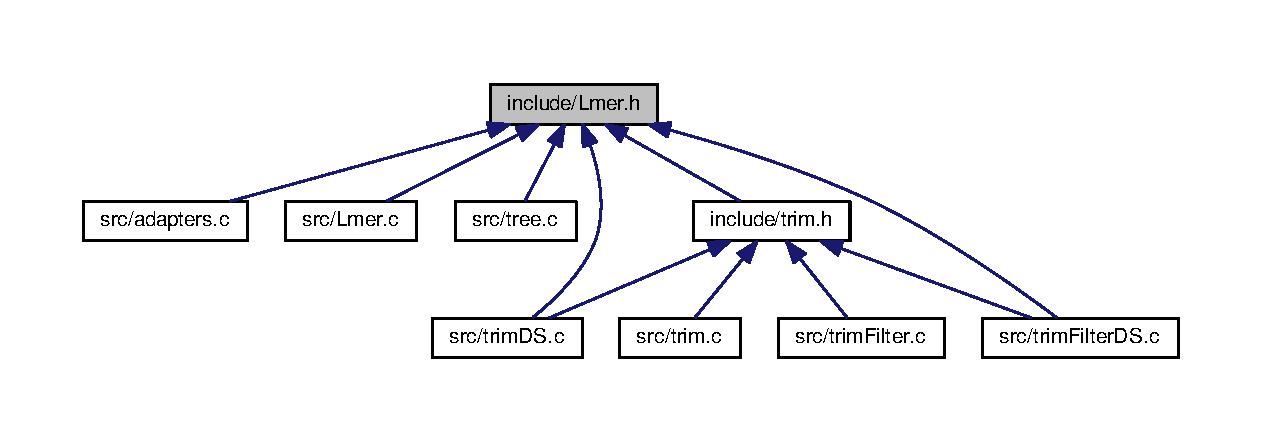
\includegraphics[width=160pt]{Lmer_8h__dep__incl}
\end{center}
\end{figure}
\subsection*{Functions}
\begin{DoxyCompactItemize}
\item 
void \hyperlink{Lmer_8h_a5f1586659681cf692359f7c8c003dd8b}{init\+\_\+map} ()
\begin{DoxyCompactList}\small\item\em Initialize lookup table L\+T. \end{DoxyCompactList}\item 
void \hyperlink{Lmer_8h_a54a9d22589c1235957b6472310280e1d}{init\+\_\+map\+\_\+\+S\+A} ()
\begin{DoxyCompactList}\small\item\em Initialize lookup table L\+T (for S\+A) \end{DoxyCompactList}\item 
\hypertarget{Lmer_8h_a3280d056532aa23523d08dfd52b60b51}{void \hyperlink{Lmer_8h_a3280d056532aa23523d08dfd52b60b51}{Lmer\+\_\+s\+Lmer} (char $\ast$Lmer, int L)}\label{Lmer_8h_a3280d056532aa23523d08dfd52b60b51}

\begin{DoxyCompactList}\small\item\em Transforms an Lmer to the convention stored in the lookup table L\+T. \end{DoxyCompactList}\item 
\hypertarget{Lmer_8h_ae4b4f0b75c0a5784ad66d856aed9d39f}{void \hyperlink{Lmer_8h_ae4b4f0b75c0a5784ad66d856aed9d39f}{rev\+\_\+comp} (char $\ast$s\+Lmer, int L)}\label{Lmer_8h_ae4b4f0b75c0a5784ad66d856aed9d39f}

\begin{DoxyCompactList}\small\item\em Obtains the reverse complement, for \{'\textbackslash{}000','\textbackslash{}001','\textbackslash{}002','\textbackslash{}003'\}. \end{DoxyCompactList}\item 
\hypertarget{Lmer_8h_a6adc3e6b4aa23ade6c889592c50c2963}{void \hyperlink{Lmer_8h_a6adc3e6b4aa23ade6c889592c50c2963}{rev\+\_\+comp2} (char $\ast$s\+Lmer, int L)}\label{Lmer_8h_a6adc3e6b4aa23ade6c889592c50c2963}

\begin{DoxyCompactList}\small\item\em Obtains the reverse complement, for \{'\textbackslash{}001','\textbackslash{}002','\textbackslash{}003','\textbackslash{}004'\}. \end{DoxyCompactList}\end{DoxyCompactItemize}


\subsection{Detailed Description}
Manipulation of Lmers and sequences. 

\begin{DoxyAuthor}{Author}
Paula Perez \href{mailto:paulaperezrubio@gmail.com}{\tt paulaperezrubio@gmail.\+com} 
\end{DoxyAuthor}
\begin{DoxyDate}{Date}
18.\+08.\+2017 
\end{DoxyDate}
\begin{DoxyNote}{Note}
I have to try to merge the two versions of conversions!
\end{DoxyNote}
Basically, and depending on the method used, nucleotides \{'a', 'c', 'g', 't'\} are shifted to the characters \{'\textbackslash{}000','\textbackslash{}001','\textbackslash{}002','\textbackslash{}003'\} or to \{'\textbackslash{}001','\textbackslash{}002','\textbackslash{}003','\textbackslash{}004'\} in a Lmer. A function to provide the reverse complement is also provided. 

\subsection{Function Documentation}
\hypertarget{Lmer_8h_a5f1586659681cf692359f7c8c003dd8b}{\index{Lmer.\+h@{Lmer.\+h}!init\+\_\+map@{init\+\_\+map}}
\index{init\+\_\+map@{init\+\_\+map}!Lmer.\+h@{Lmer.\+h}}
\subsubsection[{init\+\_\+map}]{\setlength{\rightskip}{0pt plus 5cm}void init\+\_\+map (
\begin{DoxyParamCaption}
{}
\end{DoxyParamCaption}
)}}\label{Lmer_8h_a5f1586659681cf692359f7c8c003dd8b}


Initialize lookup table L\+T. 

\{'a','c','g','t'\} --$>$ \{'\textbackslash{}000','\textbackslash{}001','\textbackslash{}002','\textbackslash{}003'\}, rest '\textbackslash{}004'. \hypertarget{Lmer_8h_a54a9d22589c1235957b6472310280e1d}{\index{Lmer.\+h@{Lmer.\+h}!init\+\_\+map\+\_\+\+S\+A@{init\+\_\+map\+\_\+\+S\+A}}
\index{init\+\_\+map\+\_\+\+S\+A@{init\+\_\+map\+\_\+\+S\+A}!Lmer.\+h@{Lmer.\+h}}
\subsubsection[{init\+\_\+map\+\_\+\+S\+A}]{\setlength{\rightskip}{0pt plus 5cm}void init\+\_\+map\+\_\+\+S\+A (
\begin{DoxyParamCaption}
{}
\end{DoxyParamCaption}
)}}\label{Lmer_8h_a54a9d22589c1235957b6472310280e1d}


Initialize lookup table L\+T (for S\+A) 

\{'a','c','g','t'\} --$>$ \{'\textbackslash{}001','\textbackslash{}002','\textbackslash{}003','\textbackslash{}004'\}, rest '\textbackslash{}005'. 
\hypertarget{Rcommand__Freport_8h}{\section{include/\+Rcommand\+\_\+\+Freport.h File Reference}
\label{Rcommand__Freport_8h}\index{include/\+Rcommand\+\_\+\+Freport.\+h@{include/\+Rcommand\+\_\+\+Freport.\+h}}
}


get Rscript command for Freport  


This graph shows which files directly or indirectly include this file\+:\nopagebreak
\begin{figure}[H]
\begin{center}
\leavevmode
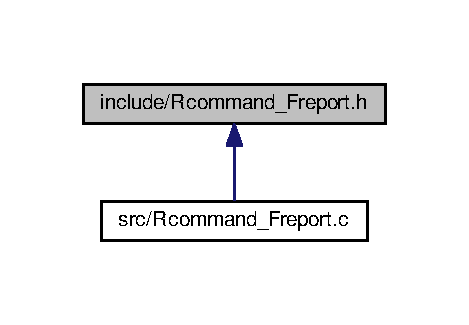
\includegraphics[width=225pt]{Rcommand__Freport_8h__dep__incl}
\end{center}
\end{figure}
\subsection*{Functions}
\begin{DoxyCompactItemize}
\item 
\hypertarget{Rcommand__Freport_8h_a9ed436a2223e2511e514557c41cd86b8}{char $\ast$ \hyperlink{Rcommand__Freport_8h_a9ed436a2223e2511e514557c41cd86b8}{command\+\_\+\+Freport} ()}\label{Rcommand__Freport_8h_a9ed436a2223e2511e514557c41cd86b8}

\begin{DoxyCompactList}\small\item\em returns Rscript command that generates the summary report in html \end{DoxyCompactList}\end{DoxyCompactItemize}


\subsection{Detailed Description}
get Rscript command for Freport 

\begin{DoxyAuthor}{Author}
Paula Perez \href{mailto:paulaperezrubio@gmail.com}{\tt paulaperezrubio@gmail.\+com} 
\end{DoxyAuthor}
\begin{DoxyDate}{Date}
01.\+09.\+2017 
\end{DoxyDate}

\hypertarget{Rcommand__Qreport_8h}{}\section{include/\+Rcommand\+\_\+\+Qreport.h File Reference}
\label{Rcommand__Qreport_8h}\index{include/\+Rcommand\+\_\+\+Qreport.\+h@{include/\+Rcommand\+\_\+\+Qreport.\+h}}


get Rscript command for Qreport  


This graph shows which files directly or indirectly include this file\+:
\nopagebreak
\begin{figure}[H]
\begin{center}
\leavevmode
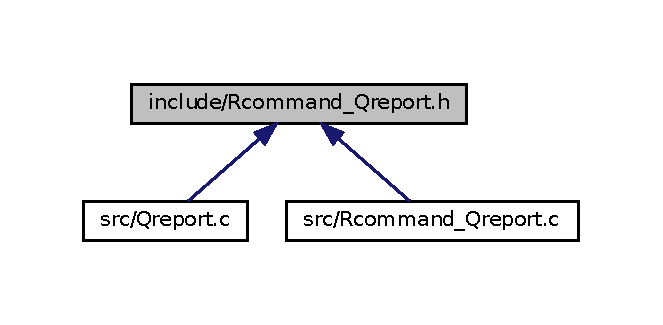
\includegraphics[width=318pt]{Rcommand__Qreport_8h__dep__incl}
\end{center}
\end{figure}
\subsection*{Functions}
\begin{DoxyCompactItemize}
\item 
\mbox{\Hypertarget{Rcommand__Qreport_8h_a336345f346ab2a993022a0ca4862731c}\label{Rcommand__Qreport_8h_a336345f346ab2a993022a0ca4862731c}} 
char $\ast$ \mbox{\hyperlink{Rcommand__Qreport_8h_a336345f346ab2a993022a0ca4862731c}{command\+\_\+\+Qreport}} ()
\begin{DoxyCompactList}\small\item\em returns Rscript command that generates the quality report in html \end{DoxyCompactList}\end{DoxyCompactItemize}


\subsection{Detailed Description}
get Rscript command for Qreport 

\begin{DoxyAuthor}{Author}
Paula Perez \href{mailto:paulaperezrubio@gmail.com}{\tt paulaperezrubio@gmail.\+com} 
\end{DoxyAuthor}
\begin{DoxyDate}{Date}
09.\+08.\+2017 
\end{DoxyDate}

\hypertarget{Rcommand__Sreport_8h}{}\section{include/\+Rcommand\+\_\+\+Sreport.h File Reference}
\label{Rcommand__Sreport_8h}\index{include/\+Rcommand\+\_\+\+Sreport.\+h@{include/\+Rcommand\+\_\+\+Sreport.\+h}}


get Rscript command for Sreport  


This graph shows which files directly or indirectly include this file\+:
\nopagebreak
\begin{figure}[H]
\begin{center}
\leavevmode
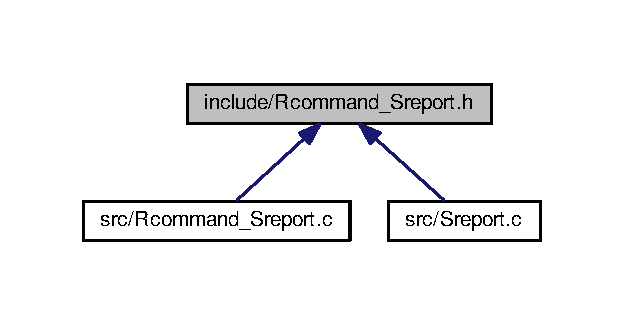
\includegraphics[width=314pt]{Rcommand__Sreport_8h__dep__incl}
\end{center}
\end{figure}
\subsection*{Functions}
\begin{DoxyCompactItemize}
\item 
char $\ast$ \mbox{\hyperlink{Rcommand__Sreport_8h_a843ffc16afb438c7430da804efd8dfaf}{command\+\_\+\+Sreport}} ()
\begin{DoxyCompactList}\small\item\em returns Rscript command that generates the summary report in html \end{DoxyCompactList}\end{DoxyCompactItemize}


\subsection{Detailed Description}
get Rscript command for Sreport 

\begin{DoxyAuthor}{Author}
Paula Perez \href{mailto:paulaperezrubio@gmail.com}{\tt paulaperezrubio@gmail.\+com} 
\end{DoxyAuthor}
\begin{DoxyDate}{Date}
09.\+08.\+2017 
\end{DoxyDate}


\subsection{Function Documentation}
\mbox{\Hypertarget{Rcommand__Sreport_8h_a843ffc16afb438c7430da804efd8dfaf}\label{Rcommand__Sreport_8h_a843ffc16afb438c7430da804efd8dfaf}} 
\index{Rcommand\+\_\+\+Sreport.\+h@{Rcommand\+\_\+\+Sreport.\+h}!command\+\_\+\+Sreport@{command\+\_\+\+Sreport}}
\index{command\+\_\+\+Sreport@{command\+\_\+\+Sreport}!Rcommand\+\_\+\+Sreport.\+h@{Rcommand\+\_\+\+Sreport.\+h}}
\subsubsection{\texorpdfstring{command\+\_\+\+Sreport()}{command\_Sreport()}}
{\footnotesize\ttfamily char$\ast$ command\+\_\+\+Sreport (\begin{DoxyParamCaption}{ }\end{DoxyParamCaption})}



returns Rscript command that generates the summary report in html 


\begin{DoxyCode}
# To run between quotation marks after:  Rscript\_RBioC -e (Rscript)
inputfolder = normalizePath( <par.SR.inputfolder>, mustWork = TRUE);
output = <par\_SR.outputfile>;
output\_file = gsub('.* /', '', output);
path = gsub('[^/]+$', '', output);
if (path != '') \{
  outputfile = paste0(normalizePath(path, mustWork = TRUE), '/', outputfile);
\} else \{
  outputfile = paste0(cwd, '/', output\_file); # cwd: current working dir
\}; 
rmarkdown::render(<par\_SR.Rmd\_file>, 
                  params = list(inputfolder = inputfolder, version= VERSION),
                  output\_file = output\_file)
\end{DoxyCode}
 
\hypertarget{stats__info_8h}{}\section{include/stats\+\_\+info.h File Reference}
\label{stats__info_8h}\index{include/stats\+\_\+info.\+h@{include/stats\+\_\+info.\+h}}


Construct the quality report variables and update them.  


{\ttfamily \#include $<$stdint.\+h$>$}\newline
{\ttfamily \#include $<$stdlib.\+h$>$}\newline
{\ttfamily \#include \char`\"{}fq\+\_\+read.\+h\char`\"{}}\newline
{\ttfamily \#include \char`\"{}defines.\+h\char`\"{}}\newline
Include dependency graph for stats\+\_\+info.\+h\+:
\nopagebreak
\begin{figure}[H]
\begin{center}
\leavevmode
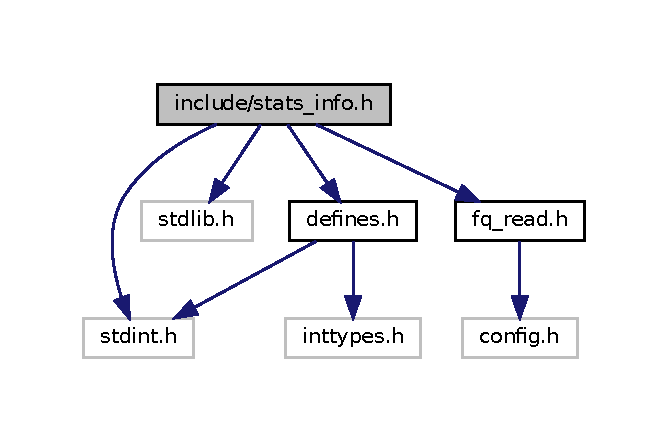
\includegraphics[width=321pt]{stats__info_8h__incl}
\end{center}
\end{figure}
This graph shows which files directly or indirectly include this file\+:
\nopagebreak
\begin{figure}[H]
\begin{center}
\leavevmode
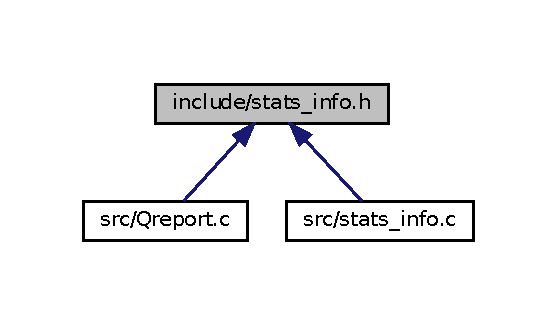
\includegraphics[width=268pt]{stats__info_8h__dep__incl}
\end{center}
\end{figure}
\subsection*{Classes}
\begin{DoxyCompactItemize}
\item 
struct \mbox{\hyperlink{structstatsinfo}{statsinfo}}
\begin{DoxyCompactList}\small\item\em stores info needed to create the summary graphs \end{DoxyCompactList}\end{DoxyCompactItemize}
\subsection*{Typedefs}
\begin{DoxyCompactItemize}
\item 
\mbox{\Hypertarget{stats__info_8h_a2671cb2f7634ad56ed3dc27446796ef1}\label{stats__info_8h_a2671cb2f7634ad56ed3dc27446796ef1}} 
typedef struct \mbox{\hyperlink{structstatsinfo}{statsinfo}} \mbox{\hyperlink{stats__info_8h_a2671cb2f7634ad56ed3dc27446796ef1}{Info}}
\begin{DoxyCompactList}\small\item\em stores info needed to create the summary graphs \end{DoxyCompactList}\end{DoxyCompactItemize}
\subsection*{Functions}
\begin{DoxyCompactItemize}
\item 
void \mbox{\hyperlink{stats__info_8h_a5c125debcca38ba396c6c01ecbc3dd5d}{init\+\_\+info}} (\mbox{\hyperlink{stats__info_8h_a2671cb2f7634ad56ed3dc27446796ef1}{Info}} $\ast$res)
\begin{DoxyCompactList}\small\item\em Initialization of a Info type. \end{DoxyCompactList}\item 
\mbox{\Hypertarget{stats__info_8h_a3354d39b533bb35891251afdb5961a3a}\label{stats__info_8h_a3354d39b533bb35891251afdb5961a3a}} 
void \mbox{\hyperlink{stats__info_8h_a3354d39b533bb35891251afdb5961a3a}{free\+\_\+info}} (\mbox{\hyperlink{stats__info_8h_a2671cb2f7634ad56ed3dc27446796ef1}{Info}} $\ast$res)
\begin{DoxyCompactList}\small\item\em frees allocated memory in Info \end{DoxyCompactList}\item 
\mbox{\Hypertarget{stats__info_8h_a7815bd5c300f89c99b539fa3e4c4f776}\label{stats__info_8h_a7815bd5c300f89c99b539fa3e4c4f776}} 
void \mbox{\hyperlink{stats__info_8h_a7815bd5c300f89c99b539fa3e4c4f776}{read\+\_\+info}} (\mbox{\hyperlink{stats__info_8h_a2671cb2f7634ad56ed3dc27446796ef1}{Info}} $\ast$res, char $\ast$file)
\begin{DoxyCompactList}\small\item\em Read Info from binary file. \end{DoxyCompactList}\item 
\mbox{\Hypertarget{stats__info_8h_ae17b550d0328a66a4941b18f24f2a920}\label{stats__info_8h_ae17b550d0328a66a4941b18f24f2a920}} 
void \mbox{\hyperlink{stats__info_8h_ae17b550d0328a66a4941b18f24f2a920}{write\+\_\+info}} (\mbox{\hyperlink{stats__info_8h_a2671cb2f7634ad56ed3dc27446796ef1}{Info}} $\ast$res, char $\ast$file)
\begin{DoxyCompactList}\small\item\em Write info to binary file. \end{DoxyCompactList}\item 
\mbox{\Hypertarget{stats__info_8h_a76d353cb30ac4cd4bc55362e7359976d}\label{stats__info_8h_a76d353cb30ac4cd4bc55362e7359976d}} 
void \mbox{\hyperlink{stats__info_8h_a76d353cb30ac4cd4bc55362e7359976d}{print\+\_\+info}} (\mbox{\hyperlink{stats__info_8h_a2671cb2f7634ad56ed3dc27446796ef1}{Info}} $\ast$res, char $\ast$infofile)
\begin{DoxyCompactList}\small\item\em print Info to a textfile \end{DoxyCompactList}\item 
\mbox{\Hypertarget{stats__info_8h_a9ca0a2ed2eb78d9a9717b82efcfdcb1f}\label{stats__info_8h_a9ca0a2ed2eb78d9a9717b82efcfdcb1f}} 
void \mbox{\hyperlink{stats__info_8h_a9ca0a2ed2eb78d9a9717b82efcfdcb1f}{get\+\_\+first\+\_\+tile}} (\mbox{\hyperlink{stats__info_8h_a2671cb2f7634ad56ed3dc27446796ef1}{Info}} $\ast$res, \mbox{\hyperlink{fq__read_8h_a9af37aa81397c9531c66863d4e97f034}{Fq\+\_\+read}} $\ast$seq)
\begin{DoxyCompactList}\small\item\em gets first tile \end{DoxyCompactList}\item 
\mbox{\Hypertarget{stats__info_8h_af599aaaf2eb242dcb6e9f44c0eb8c180}\label{stats__info_8h_af599aaaf2eb242dcb6e9f44c0eb8c180}} 
void \mbox{\hyperlink{stats__info_8h_af599aaaf2eb242dcb6e9f44c0eb8c180}{update\+\_\+info}} (\mbox{\hyperlink{stats__info_8h_a2671cb2f7634ad56ed3dc27446796ef1}{Info}} $\ast$res, \mbox{\hyperlink{fq__read_8h_a9af37aa81397c9531c66863d4e97f034}{Fq\+\_\+read}} $\ast$seq)
\begin{DoxyCompactList}\small\item\em updates Info with Fq\+\_\+read \end{DoxyCompactList}\item 
int \mbox{\hyperlink{stats__info_8h_a5bceee4c9ce4858a2e1a1022020f3051}{update\+\_\+\+A\+C\+G\+T\+\_\+counts}} (uint64\+\_\+t $\ast$A\+C\+G\+T\+\_\+low, char A\+C\+GT)
\begin{DoxyCompactList}\small\item\em update, for current tile, A\+C\+GT counts. \end{DoxyCompactList}\item 
\mbox{\Hypertarget{stats__info_8h_a12859b5ec4a85f24df22833b2ddeee79}\label{stats__info_8h_a12859b5ec4a85f24df22833b2ddeee79}} 
void \mbox{\hyperlink{stats__info_8h_a12859b5ec4a85f24df22833b2ddeee79}{update\+\_\+\+Q\+Pos\+Tile\+\_\+table}} (\mbox{\hyperlink{stats__info_8h_a2671cb2f7634ad56ed3dc27446796ef1}{Info}} $\ast$res, \mbox{\hyperlink{fq__read_8h_a9af37aa81397c9531c66863d4e97f034}{Fq\+\_\+read}} $\ast$seq)
\begin{DoxyCompactList}\small\item\em update Q\+Postile table \end{DoxyCompactList}\item 
\mbox{\Hypertarget{stats__info_8h_a89eaadfa007bf08a3d3b5b6dcda9ae37}\label{stats__info_8h_a89eaadfa007bf08a3d3b5b6dcda9ae37}} 
void \mbox{\hyperlink{stats__info_8h_a89eaadfa007bf08a3d3b5b6dcda9ae37}{update\+\_\+\+A\+C\+G\+T\+\_\+pos}} (uint64\+\_\+t $\ast$A\+C\+G\+T\+\_\+pos, \mbox{\hyperlink{fq__read_8h_a9af37aa81397c9531c66863d4e97f034}{Fq\+\_\+read}} $\ast$seq)
\begin{DoxyCompactList}\small\item\em update A\+C\+G\+T\+\_\+pos \end{DoxyCompactList}\item 
void \mbox{\hyperlink{stats__info_8h_a8ca7ce52d36a35e78b8c0bde089aedcf}{resize\+\_\+info}} (\mbox{\hyperlink{stats__info_8h_a2671cb2f7634ad56ed3dc27446796ef1}{Info}} $\ast$res)
\begin{DoxyCompactList}\small\item\em resize Info \end{DoxyCompactList}\end{DoxyCompactItemize}


\subsection{Detailed Description}
Construct the quality report variables and update them. 

\begin{DoxyAuthor}{Author}
Paula Perez \href{mailto:paulaperezrubio@gmail.com}{\tt paulaperezrubio@gmail.\+com} 
\end{DoxyAuthor}
\begin{DoxyDate}{Date}
04.\+08.\+2017 
\end{DoxyDate}


\subsection{Function Documentation}
\mbox{\Hypertarget{stats__info_8h_a5c125debcca38ba396c6c01ecbc3dd5d}\label{stats__info_8h_a5c125debcca38ba396c6c01ecbc3dd5d}} 
\index{stats\+\_\+info.\+h@{stats\+\_\+info.\+h}!init\+\_\+info@{init\+\_\+info}}
\index{init\+\_\+info@{init\+\_\+info}!stats\+\_\+info.\+h@{stats\+\_\+info.\+h}}
\subsubsection{\texorpdfstring{init\+\_\+info()}{init\_info()}}
{\footnotesize\ttfamily void init\+\_\+info (\begin{DoxyParamCaption}\item[{\mbox{\hyperlink{stats__info_8h_a2671cb2f7634ad56ed3dc27446796ef1}{Info}} $\ast$}]{res }\end{DoxyParamCaption})}



Initialization of a Info type. 

It sets\+: nQ, read\+\_\+len, ntiles, minQ and the dimensions of the arrays. Initializes the rest of the variables to zero and allocates memory to the arrays initializing them to 0 (calloc). \mbox{\Hypertarget{stats__info_8h_a8ca7ce52d36a35e78b8c0bde089aedcf}\label{stats__info_8h_a8ca7ce52d36a35e78b8c0bde089aedcf}} 
\index{stats\+\_\+info.\+h@{stats\+\_\+info.\+h}!resize\+\_\+info@{resize\+\_\+info}}
\index{resize\+\_\+info@{resize\+\_\+info}!stats\+\_\+info.\+h@{stats\+\_\+info.\+h}}
\subsubsection{\texorpdfstring{resize\+\_\+info()}{resize\_info()}}
{\footnotesize\ttfamily void resize\+\_\+info (\begin{DoxyParamCaption}\item[{\mbox{\hyperlink{stats__info_8h_a2671cb2f7634ad56ed3dc27446796ef1}{Info}} $\ast$}]{res }\end{DoxyParamCaption})}



resize Info 

At the end of the program, resize the structure Info, and adapt it to the actual number of tiles and the actual number of different quality values present. \mbox{\Hypertarget{stats__info_8h_a5bceee4c9ce4858a2e1a1022020f3051}\label{stats__info_8h_a5bceee4c9ce4858a2e1a1022020f3051}} 
\index{stats\+\_\+info.\+h@{stats\+\_\+info.\+h}!update\+\_\+\+A\+C\+G\+T\+\_\+counts@{update\+\_\+\+A\+C\+G\+T\+\_\+counts}}
\index{update\+\_\+\+A\+C\+G\+T\+\_\+counts@{update\+\_\+\+A\+C\+G\+T\+\_\+counts}!stats\+\_\+info.\+h@{stats\+\_\+info.\+h}}
\subsubsection{\texorpdfstring{update\+\_\+\+A\+C\+G\+T\+\_\+counts()}{update\_ACGT\_counts()}}
{\footnotesize\ttfamily int update\+\_\+\+A\+C\+G\+T\+\_\+counts (\begin{DoxyParamCaption}\item[{uint64\+\_\+t $\ast$}]{A\+C\+G\+T\+\_\+low,  }\item[{char}]{A\+C\+GT }\end{DoxyParamCaption})}



update, for current tile, A\+C\+GT counts. 

Makes update of A\+C\+GT counts for the current tile. Can be used with variables\+: low\+Q\+\_\+\+A\+C\+G\+T\+\_\+tile and A\+C\+G\+T\+\_\+tile 
\hypertarget{str__manip_8h}{\section{include/str\+\_\+manip.h File Reference}
\label{str__manip_8h}\index{include/str\+\_\+manip.\+h@{include/str\+\_\+manip.\+h}}
}


functions that do string manipulation  


This graph shows which files directly or indirectly include this file\+:\nopagebreak
\begin{figure}[H]
\begin{center}
\leavevmode
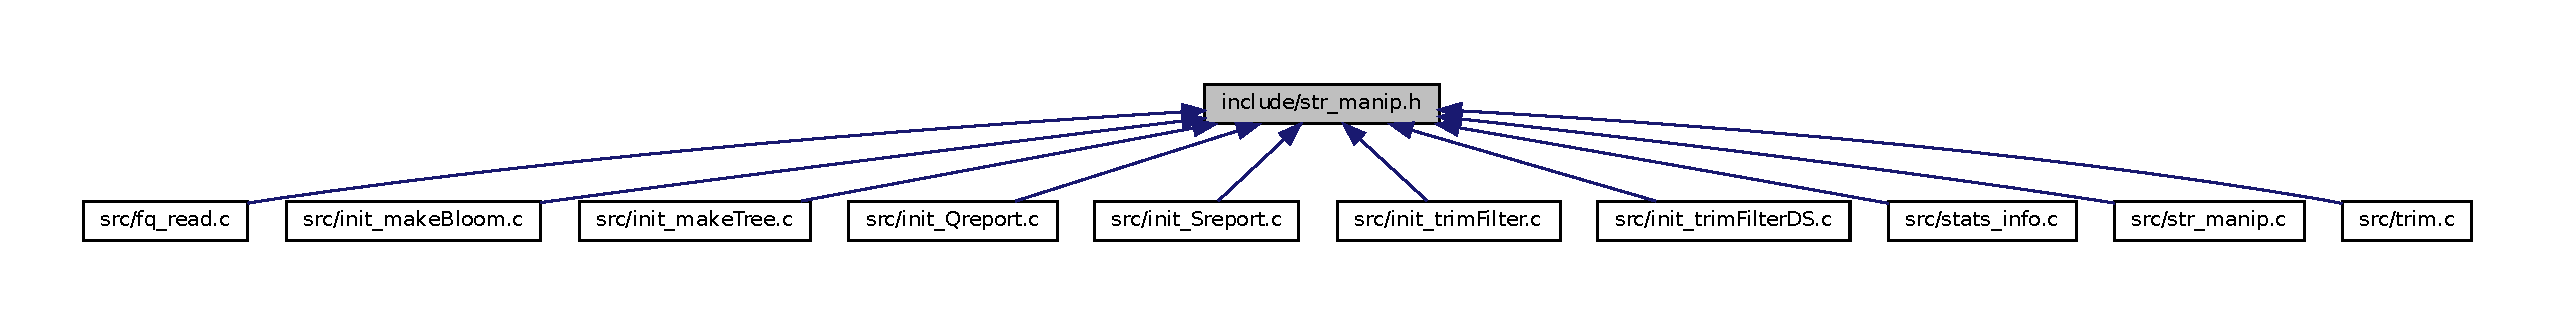
\includegraphics[width=350pt]{str__manip_8h__dep__incl}
\end{center}
\end{figure}
\subsection*{Classes}
\begin{DoxyCompactItemize}
\item 
struct \hyperlink{struct__split}{\+\_\+split}
\begin{DoxyCompactList}\small\item\em contains a splitted string and the number or splitted fields \end{DoxyCompactList}\end{DoxyCompactItemize}
\subsection*{Typedefs}
\begin{DoxyCompactItemize}
\item 
\hypertarget{str__manip_8h_aeff63a40ce3fff0c51bd207baeba2013}{typedef struct \hyperlink{struct__split}{\+\_\+split} \hyperlink{str__manip_8h_aeff63a40ce3fff0c51bd207baeba2013}{Split}}\label{str__manip_8h_aeff63a40ce3fff0c51bd207baeba2013}

\begin{DoxyCompactList}\small\item\em contains a splitted string and the number or splitted fields \end{DoxyCompactList}\end{DoxyCompactItemize}
\subsection*{Functions}
\begin{DoxyCompactItemize}
\item 
\hypertarget{str__manip_8h_a15e8cbc96aa4cea159dbc59d1c01ffaa}{int \hyperlink{str__manip_8h_a15e8cbc96aa4cea159dbc59d1c01ffaa}{str\+\_\+isascii} (char $\ast$s)}\label{str__manip_8h_a15e8cbc96aa4cea159dbc59d1c01ffaa}

\begin{DoxyCompactList}\small\item\em return nonzero iff all elements in the string are in the A\+S\+C\+I\+I set. \end{DoxyCompactList}\item 
int \hyperlink{str__manip_8h_a8108ab52dfbc1af644bf7682c1bbe33f}{strindex} (char $\ast$s, char $\ast$t)
\begin{DoxyCompactList}\small\item\em returns index of t in s (start, first occurence) \end{DoxyCompactList}\item 
\hypertarget{str__manip_8h_af8d13ec7edfe3ca8a03f48bd7e3b1d83}{int \hyperlink{str__manip_8h_af8d13ec7edfe3ca8a03f48bd7e3b1d83}{count\+\_\+char} (char $\ast$s, char c)}\label{str__manip_8h_af8d13ec7edfe3ca8a03f48bd7e3b1d83}

\begin{DoxyCompactList}\small\item\em returns the \# of occurences of char c in string s \end{DoxyCompactList}\item 
\hyperlink{str__manip_8h_aeff63a40ce3fff0c51bd207baeba2013}{Split} \hyperlink{str__manip_8h_a245675aede3b8bedd8ce6c8c2aa70ec0}{strsplit} (char $\ast$str, char sep)
\begin{DoxyCompactList}\small\item\em Separates strings by a separator. \end{DoxyCompactList}\end{DoxyCompactItemize}


\subsection{Detailed Description}
functions that do string manipulation 

\begin{DoxyAuthor}{Author}
Paula Perez \href{mailto:paulaperezrubio@gmail.com}{\tt paulaperezrubio@gmail.\+com} 
\end{DoxyAuthor}
\begin{DoxyDate}{Date}
03.\+08.\+2017 
\end{DoxyDate}


\subsection{Function Documentation}
\hypertarget{str__manip_8h_a8108ab52dfbc1af644bf7682c1bbe33f}{\index{str\+\_\+manip.\+h@{str\+\_\+manip.\+h}!strindex@{strindex}}
\index{strindex@{strindex}!str\+\_\+manip.\+h@{str\+\_\+manip.\+h}}
\subsubsection[{strindex}]{\setlength{\rightskip}{0pt plus 5cm}int strindex (
\begin{DoxyParamCaption}
\item[{char $\ast$}]{s, }
\item[{char $\ast$}]{t}
\end{DoxyParamCaption}
)}}\label{str__manip_8h_a8108ab52dfbc1af644bf7682c1bbe33f}


returns index of t in s (start, first occurence) 


\begin{DoxyParams}{Parameters}
{\em s} & string to be checked. \\
\hline
{\em t} & substring to be found in s. \\
\hline
\end{DoxyParams}
\hypertarget{str__manip_8h_a245675aede3b8bedd8ce6c8c2aa70ec0}{\index{str\+\_\+manip.\+h@{str\+\_\+manip.\+h}!strsplit@{strsplit}}
\index{strsplit@{strsplit}!str\+\_\+manip.\+h@{str\+\_\+manip.\+h}}
\subsubsection[{strsplit}]{\setlength{\rightskip}{0pt plus 5cm}{\bf Split} strsplit (
\begin{DoxyParamCaption}
\item[{char $\ast$}]{str, }
\item[{char}]{sep}
\end{DoxyParamCaption}
)}}\label{str__manip_8h_a245675aede3b8bedd8ce6c8c2aa70ec0}


Separates strings by a separator. 


\begin{DoxyParams}{Parameters}
{\em str} & input string \\
\hline
{\em sep} & separator (char) \\
\hline
\end{DoxyParams}
\begin{DoxyReturn}{Returns}
array of strings containing the substrings in the input separated 
\end{DoxyReturn}

\hypertarget{tree_8h}{\section{include/tree.h File Reference}
\label{tree_8h}\index{include/tree.\+h@{include/tree.\+h}}
}


Construction of tree, check paths, write tree, read in tree.  


{\ttfamily \#include $<$stdint.\+h$>$}\\*
{\ttfamily \#include \char`\"{}defines.\+h\char`\"{}}\\*
{\ttfamily \#include \char`\"{}fa\+\_\+read.\+h\char`\"{}}\\*
Include dependency graph for tree.\+h\+:\nopagebreak
\begin{figure}[H]
\begin{center}
\leavevmode
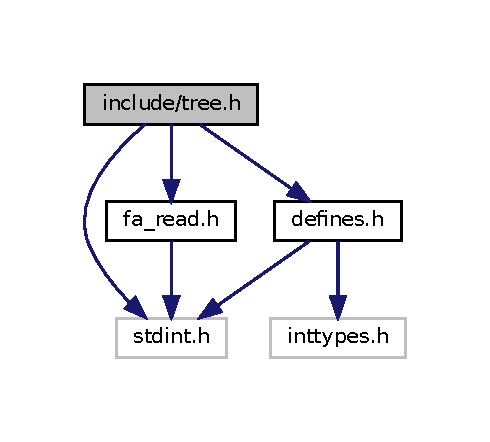
\includegraphics[width=223pt]{tree_8h__incl}
\end{center}
\end{figure}
This graph shows which files directly or indirectly include this file\+:\nopagebreak
\begin{figure}[H]
\begin{center}
\leavevmode
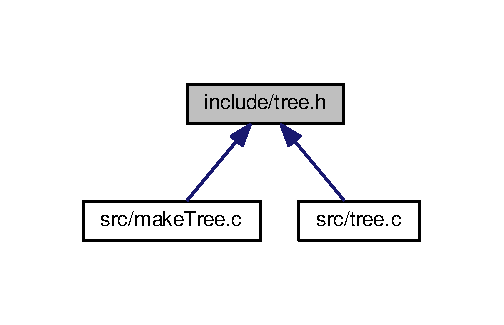
\includegraphics[width=350pt]{tree_8h__dep__incl}
\end{center}
\end{figure}
\subsection*{Classes}
\begin{DoxyCompactItemize}
\item 
struct \hyperlink{struct__node}{\+\_\+node}
\begin{DoxyCompactList}\small\item\em Node structure\+: formed out of T\+\_\+\+A\+C\+G\+T pointers to Node structure. \end{DoxyCompactList}\item 
struct \hyperlink{struct__tree}{\+\_\+tree}
\begin{DoxyCompactList}\small\item\em structure containing a T\+\_\+\+A\+C\+G\+T-\/tree. \end{DoxyCompactList}\end{DoxyCompactItemize}
\subsection*{Typedefs}
\begin{DoxyCompactItemize}
\item 
\hypertarget{tree_8h_a6390a1d02010dee1843fa2b1263308c1}{typedef struct \hyperlink{struct__node}{\+\_\+node} \hyperlink{tree_8h_a6390a1d02010dee1843fa2b1263308c1}{Node}}\label{tree_8h_a6390a1d02010dee1843fa2b1263308c1}

\begin{DoxyCompactList}\small\item\em Node structure\+: formed out of T\+\_\+\+A\+C\+G\+T pointers to Node structure. \end{DoxyCompactList}\item 
typedef struct \hyperlink{struct__tree}{\+\_\+tree} \hyperlink{tree_8h_a50a06950fa1e82738ad9a6bd85914900}{Tree}
\begin{DoxyCompactList}\small\item\em structure containing a T\+\_\+\+A\+C\+G\+T-\/tree. \end{DoxyCompactList}\end{DoxyCompactItemize}
\subsection*{Functions}
\begin{DoxyCompactItemize}
\item 
\hyperlink{tree_8h_a6390a1d02010dee1843fa2b1263308c1}{Node} $\ast$ \hyperlink{tree_8h_a759333d12a4ed298504cc08c69a19a27}{get\+\_\+new\+\_\+pool} (\hyperlink{tree_8h_a50a06950fa1e82738ad9a6bd85914900}{Tree} $\ast$tree\+\_\+ptr)
\begin{DoxyCompactList}\small\item\em reallocs pool\+\_\+2\+D (++\+N\+P\+O\+O\+L\+\_\+2\+D) if all existing nodes have been used \end{DoxyCompactList}\item 
\hyperlink{tree_8h_a6390a1d02010dee1843fa2b1263308c1}{Node} $\ast$ \hyperlink{tree_8h_a407b006b6b9c55cc8ef07c670becce33}{new\+\_\+node\+\_\+buf} (\hyperlink{tree_8h_a50a06950fa1e82738ad9a6bd85914900}{Tree} $\ast$tree\+\_\+ptr)
\begin{DoxyCompactList}\small\item\em moves to the next node (allocating new memory if necessary) \end{DoxyCompactList}\item 
void \hyperlink{tree_8h_a9bf758d5738d90a332fcd04485853d84}{free\+\_\+all\+\_\+nodes} (\hyperlink{tree_8h_a50a06950fa1e82738ad9a6bd85914900}{Tree} $\ast$tree\+\_\+ptr)
\begin{DoxyCompactList}\small\item\em frees the whole tree structure \end{DoxyCompactList}\item 
\hypertarget{tree_8h_a3cd8ebe19e5c6e6b54771eede75c935b}{void \hyperlink{tree_8h_a3cd8ebe19e5c6e6b54771eede75c935b}{insert\+\_\+\+Lmer} (\hyperlink{tree_8h_a50a06950fa1e82738ad9a6bd85914900}{Tree} $\ast$tree\+\_\+ptr, char $\ast$Lmer)}\label{tree_8h_a3cd8ebe19e5c6e6b54771eede75c935b}

\begin{DoxyCompactList}\small\item\em Lmer insertion in the tree (depth L). \end{DoxyCompactList}\item 
\hypertarget{tree_8h_a5f428a722fa118b5f4684fd06401db9a}{void \hyperlink{tree_8h_a5f428a722fa118b5f4684fd06401db9a}{insert\+\_\+entry} (\hyperlink{tree_8h_a50a06950fa1e82738ad9a6bd85914900}{Tree} $\ast$tree\+\_\+ptr, \hyperlink{fa__read_8h_a8f68b28ad3a6c33fe1dd78d5ac044b30}{Fa\+\_\+entry} $\ast$entry)}\label{tree_8h_a5f428a722fa118b5f4684fd06401db9a}

\begin{DoxyCompactList}\small\item\em fasta entry insertion in the tree (depth L). \end{DoxyCompactList}\item 
double \hyperlink{tree_8h_a7ea4e8b262dc61c20d94b598bffab181}{check\+\_\+path} (\hyperlink{tree_8h_a50a06950fa1e82738ad9a6bd85914900}{Tree} $\ast$tree\+\_\+ptr, char $\ast$read, int Lread)
\begin{DoxyCompactList}\small\item\em checks if read is found in tree and outputs a score \end{DoxyCompactList}\item 
\hyperlink{tree_8h_a50a06950fa1e82738ad9a6bd85914900}{Tree} $\ast$ \hyperlink{tree_8h_a3cec782fc1e0ae4063a34c641b463f89}{tree\+\_\+from\+\_\+fasta} (\hyperlink{fa__read_8h_a797328b16bc1c1088998cd164aafb09d}{Fa\+\_\+data} $\ast$fasta, int L)
\begin{DoxyCompactList}\small\item\em create Tree structure from fasta structure. \end{DoxyCompactList}\item 
void \hyperlink{tree_8h_a3b6ea3f3ef0c84a182e93a58ea417aea}{save\+\_\+tree} (\hyperlink{tree_8h_a50a06950fa1e82738ad9a6bd85914900}{Tree} $\ast$tree\+\_\+ptr, char $\ast$filename)
\begin{DoxyCompactList}\small\item\em saves Tree to disk in filename \end{DoxyCompactList}\item 
\hyperlink{tree_8h_a50a06950fa1e82738ad9a6bd85914900}{Tree} $\ast$ \hyperlink{tree_8h_a58f15d601ef34104e008d0ff8cb28bee}{read\+\_\+tree} (char $\ast$filename)
\begin{DoxyCompactList}\small\item\em read tree from file \end{DoxyCompactList}\end{DoxyCompactItemize}


\subsection{Detailed Description}
Construction of tree, check paths, write tree, read in tree. 

\begin{DoxyAuthor}{Author}
Paula Perez \href{mailto:paulaperezrubio@gmail.com}{\tt paulaperezrubio@gmail.\+com} 
\end{DoxyAuthor}
\begin{DoxyDate}{Date}
18.\+08.\+2017 
\end{DoxyDate}


\subsection{Typedef Documentation}
\hypertarget{tree_8h_a50a06950fa1e82738ad9a6bd85914900}{\index{tree.\+h@{tree.\+h}!Tree@{Tree}}
\index{Tree@{Tree}!tree.\+h@{tree.\+h}}
\subsubsection[{Tree}]{\setlength{\rightskip}{0pt plus 5cm}typedef struct {\bf \+\_\+tree}  {\bf Tree}}}\label{tree_8h_a50a06950fa1e82738ad9a6bd85914900}


structure containing a T\+\_\+\+A\+C\+G\+T-\/tree. 

The tree structure is stored in a pointer to pointer to Node. We grow the structure on the flight as we need more memory. In the outer direction, we start by allocating N\+P\+O\+O\+L\+\_\+2\+D pointers to Node. In the inner direction, we allocate N\+P\+O\+O\+L\+\_\+1\+D Nodes and fill them as we read the fasta file. When all of them are allocated, we allocate again N\+P\+O\+O\+L\+\_\+1\+D. If N\+P\+O\+O\+L\+\_\+2\+D pointers to Node are allocated, the outer dimension is reallocated with +\+N\+P\+O\+O\+L\+\_\+2\+D extra elements. L is the depth of the tree, pool\+\_\+count is the number on Node$\ast$ elements used so far, pool\+\_\+available is the number of Nodes available in every moment, and nnodes is the total number of nodes filled in. We limit the number of allocated nodes to U\+I\+N\+T\+\_\+\+M\+A\+X (we cannot count more nodes!). 

\subsection{Function Documentation}
\hypertarget{tree_8h_a7ea4e8b262dc61c20d94b598bffab181}{\index{tree.\+h@{tree.\+h}!check\+\_\+path@{check\+\_\+path}}
\index{check\+\_\+path@{check\+\_\+path}!tree.\+h@{tree.\+h}}
\subsubsection[{check\+\_\+path}]{\setlength{\rightskip}{0pt plus 5cm}double check\+\_\+path (
\begin{DoxyParamCaption}
\item[{{\bf Tree} $\ast$}]{tree\+\_\+ptr, }
\item[{char $\ast$}]{read, }
\item[{int}]{Lread}
\end{DoxyParamCaption}
)}}\label{tree_8h_a7ea4e8b262dc61c20d94b598bffab181}


checks if read is found in tree and outputs a score 


\begin{DoxyParams}{Parameters}
{\em tree\+\_\+ptr} & pointer to Tree structure \\
\hline
{\em read} & Read or reverse complement \\
\hline
{\em Lread} & length of read \\
\hline
\end{DoxyParams}
\begin{DoxyReturn}{Returns}
score = (number of Lmers of reads found in read) / (Lread-\/\+L+1) 
\end{DoxyReturn}
\hypertarget{tree_8h_a9bf758d5738d90a332fcd04485853d84}{\index{tree.\+h@{tree.\+h}!free\+\_\+all\+\_\+nodes@{free\+\_\+all\+\_\+nodes}}
\index{free\+\_\+all\+\_\+nodes@{free\+\_\+all\+\_\+nodes}!tree.\+h@{tree.\+h}}
\subsubsection[{free\+\_\+all\+\_\+nodes}]{\setlength{\rightskip}{0pt plus 5cm}void free\+\_\+all\+\_\+nodes (
\begin{DoxyParamCaption}
\item[{{\bf Tree} $\ast$}]{tree\+\_\+ptr}
\end{DoxyParamCaption}
)}}\label{tree_8h_a9bf758d5738d90a332fcd04485853d84}


frees the whole tree structure 


\begin{DoxyParams}{Parameters}
{\em tree\+\_\+ptr} & pointer to Tree structure\\
\hline
\end{DoxyParams}
This function deallocates the memory allocated in a Tree structure. \hypertarget{tree_8h_a759333d12a4ed298504cc08c69a19a27}{\index{tree.\+h@{tree.\+h}!get\+\_\+new\+\_\+pool@{get\+\_\+new\+\_\+pool}}
\index{get\+\_\+new\+\_\+pool@{get\+\_\+new\+\_\+pool}!tree.\+h@{tree.\+h}}
\subsubsection[{get\+\_\+new\+\_\+pool}]{\setlength{\rightskip}{0pt plus 5cm}{\bf Node}$\ast$ get\+\_\+new\+\_\+pool (
\begin{DoxyParamCaption}
\item[{{\bf Tree} $\ast$}]{tree\+\_\+ptr}
\end{DoxyParamCaption}
)}}\label{tree_8h_a759333d12a4ed298504cc08c69a19a27}


reallocs pool\+\_\+2\+D (++\+N\+P\+O\+O\+L\+\_\+2\+D) if all existing nodes have been used 


\begin{DoxyParams}{Parameters}
{\em tree\+\_\+ptr} & pointer to Tree structure \\
\hline
\end{DoxyParams}
\hypertarget{tree_8h_a407b006b6b9c55cc8ef07c670becce33}{\index{tree.\+h@{tree.\+h}!new\+\_\+node\+\_\+buf@{new\+\_\+node\+\_\+buf}}
\index{new\+\_\+node\+\_\+buf@{new\+\_\+node\+\_\+buf}!tree.\+h@{tree.\+h}}
\subsubsection[{new\+\_\+node\+\_\+buf}]{\setlength{\rightskip}{0pt plus 5cm}{\bf Node}$\ast$ new\+\_\+node\+\_\+buf (
\begin{DoxyParamCaption}
\item[{{\bf Tree} $\ast$}]{tree\+\_\+ptr}
\end{DoxyParamCaption}
)}}\label{tree_8h_a407b006b6b9c55cc8ef07c670becce33}


moves to the next node (allocating new memory if necessary) 


\begin{DoxyParams}{Parameters}
{\em tree\+\_\+ptr} & pointer to Tree structure \\
\hline
\end{DoxyParams}
\begin{DoxyReturn}{Returns}
address to next node
\end{DoxyReturn}
The function checks if there are available nodes (information stored in the variable tree\+\_\+ptr -\/$>$ pool\+\_\+available) and goes to the next node. If there is no nodes left, it allocates a new pool\+\_\+1\+D, and if there is no room left in the outter dimension, it reallocates N\+P\+O\+O\+L\+\_\+2\+D more Node$\ast$'s. If the number of nodes reaches U\+I\+N\+T\+\_\+\+M\+A\+X, the program returns an error message and exits. \hypertarget{tree_8h_a58f15d601ef34104e008d0ff8cb28bee}{\index{tree.\+h@{tree.\+h}!read\+\_\+tree@{read\+\_\+tree}}
\index{read\+\_\+tree@{read\+\_\+tree}!tree.\+h@{tree.\+h}}
\subsubsection[{read\+\_\+tree}]{\setlength{\rightskip}{0pt plus 5cm}{\bf Tree}$\ast$ read\+\_\+tree (
\begin{DoxyParamCaption}
\item[{char $\ast$}]{filename}
\end{DoxyParamCaption}
)}}\label{tree_8h_a58f15d601ef34104e008d0ff8cb28bee}


read tree from file 


\begin{DoxyParams}{Parameters}
{\em filename} & string with the filename \\
\hline
\end{DoxyParams}
\begin{DoxyReturn}{Returns}
pointer to Tree structure
\end{DoxyReturn}
This function unwinds the process carried out in save\+\_\+tree and assigns addresses to the children of every given node. \hypertarget{tree_8h_a3b6ea3f3ef0c84a182e93a58ea417aea}{\index{tree.\+h@{tree.\+h}!save\+\_\+tree@{save\+\_\+tree}}
\index{save\+\_\+tree@{save\+\_\+tree}!tree.\+h@{tree.\+h}}
\subsubsection[{save\+\_\+tree}]{\setlength{\rightskip}{0pt plus 5cm}void save\+\_\+tree (
\begin{DoxyParamCaption}
\item[{{\bf Tree} $\ast$}]{tree\+\_\+ptr, }
\item[{char $\ast$}]{filename}
\end{DoxyParamCaption}
)}}\label{tree_8h_a3b6ea3f3ef0c84a182e93a58ea417aea}


saves Tree to disk in filename 


\begin{DoxyParams}{Parameters}
{\em tree\+\_\+ptr} & pointer to Tree structure \\
\hline
{\em filename} & string containing filename\\
\hline
\end{DoxyParams}
The tree structure is stored as follows\+: every address is stored in a uint32\+\_\+t (we are not allowing trees with more than U\+I\+N\+T\+\_\+\+M\+A\+X nodes). For every node, the addresses of the children are stored in the following fashion\+:
\begin{DoxyItemize}
\item If it is pointing to N\+U\+L\+L\+: 0.
\item Otherwise\+: i2, the index in the outer dimension of pool\+\_\+2\+D is identified, and the difference jump = pool\+\_\+2\+D\mbox{[}i\mbox{]}\mbox{[}j\mbox{]}.children\mbox{[}k\mbox{]} -\/ pool\+\_\+2\+D\mbox{[}i2\mbox{]} is computed. i2$\ast$\+N\+P\+O\+O\+L\+\_\+\+D1 + jump is then stored for child k. 
\end{DoxyItemize}\hypertarget{tree_8h_a3cec782fc1e0ae4063a34c641b463f89}{\index{tree.\+h@{tree.\+h}!tree\+\_\+from\+\_\+fasta@{tree\+\_\+from\+\_\+fasta}}
\index{tree\+\_\+from\+\_\+fasta@{tree\+\_\+from\+\_\+fasta}!tree.\+h@{tree.\+h}}
\subsubsection[{tree\+\_\+from\+\_\+fasta}]{\setlength{\rightskip}{0pt plus 5cm}{\bf Tree}$\ast$ tree\+\_\+from\+\_\+fasta (
\begin{DoxyParamCaption}
\item[{{\bf Fa\+\_\+data} $\ast$}]{fasta, }
\item[{int}]{L}
\end{DoxyParamCaption}
)}}\label{tree_8h_a3cec782fc1e0ae4063a34c641b463f89}


create Tree structure from fasta structure. 


\begin{DoxyParams}{Parameters}
{\em fasta} & pointer to fasta structure \\
\hline
{\em L} & tree length \\
\hline
\end{DoxyParams}

\hypertarget{trim_8h}{\section{include/trim.h File Reference}
\label{trim_8h}\index{include/trim.\+h@{include/trim.\+h}}
}


trims/filter sequences after Quality, N's contaminations.  


{\ttfamily \#include $<$stdio.\+h$>$}\\*
{\ttfamily \#include \char`\"{}Lmer.\+h\char`\"{}}\\*
{\ttfamily \#include \char`\"{}fq\+\_\+read.\+h\char`\"{}}\\*
{\ttfamily \#include \char`\"{}defines.\+h\char`\"{}}\\*
{\ttfamily \#include \char`\"{}tree.\+h\char`\"{}}\\*
{\ttfamily \#include \char`\"{}bloom.\+h\char`\"{}}\\*
{\ttfamily \#include \char`\"{}adapters.\+h\char`\"{}}\\*
Include dependency graph for trim.\+h\+:\nopagebreak
\begin{figure}[H]
\begin{center}
\leavevmode
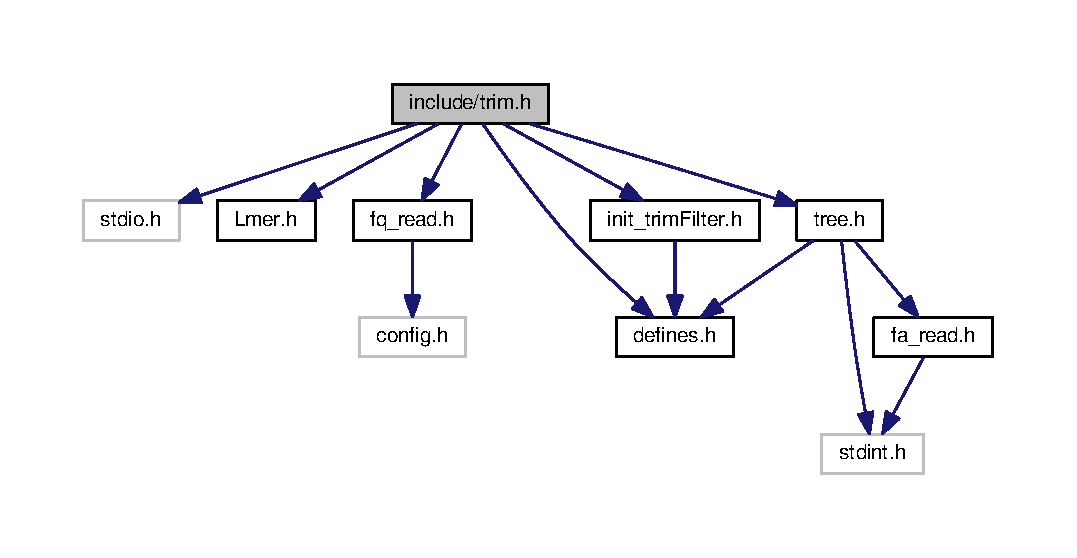
\includegraphics[width=350pt]{trim_8h__incl}
\end{center}
\end{figure}
This graph shows which files directly or indirectly include this file\+:\nopagebreak
\begin{figure}[H]
\begin{center}
\leavevmode
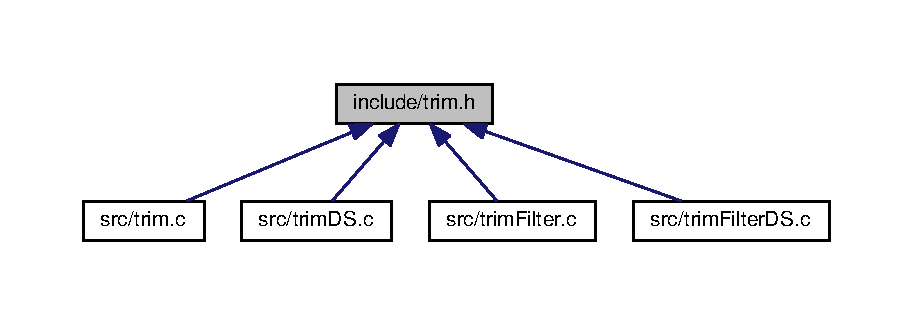
\includegraphics[width=350pt]{trim_8h__dep__incl}
\end{center}
\end{figure}
\subsection*{Functions}
\begin{DoxyCompactItemize}
\item 
int \hyperlink{trim_8h_aed995029d7181d69875b2dee0d7b6ce9}{trim\+\_\+adapter} (\hyperlink{fq__read_8h_a9af37aa81397c9531c66863d4e97f034}{Fq\+\_\+read} $\ast$seq, \hyperlink{adapters_8h_ad1465e8f3bc3d3b1fc010a1e72436c56}{Ad\+\_\+seq} $\ast$adap\+\_\+list)
\begin{DoxyCompactList}\small\item\em trims sequence based on presence of N nucleotides \end{DoxyCompactList}\item 
int \hyperlink{trim_8h_af23d3685193b624b72a6969a49903a97}{trim\+\_\+sequence\+N} (\hyperlink{fq__read_8h_a9af37aa81397c9531c66863d4e97f034}{Fq\+\_\+read} $\ast$seq)
\begin{DoxyCompactList}\small\item\em trims sequence based on presence of N nucleotides \end{DoxyCompactList}\item 
int \hyperlink{trim_8h_ae5ab2bb79068d8a7e0d72686c1f50320}{trim\+\_\+sequence\+Q} (\hyperlink{fq__read_8h_a9af37aa81397c9531c66863d4e97f034}{Fq\+\_\+read} $\ast$seq)
\begin{DoxyCompactList}\small\item\em trims sequence based on low\+Q base callings \end{DoxyCompactList}\item 
\hyperlink{defines_8h_abb452686968e48b67397da5f97445f5b}{bool} \hyperlink{trim_8h_a7e2b4015298659b7e21a80d4bb031e2f}{is\+\_\+read\+\_\+in\+Tree} (\hyperlink{tree_8h_a50a06950fa1e82738ad9a6bd85914900}{Tree} $\ast$tree\+\_\+ptr, \hyperlink{fq__read_8h_a9af37aa81397c9531c66863d4e97f034}{Fq\+\_\+read} $\ast$seq)
\begin{DoxyCompactList}\small\item\em check if Lread is contained in tree. It computes the score for the read and its reverse complement; if one ot them exceeds the user selected threshold, it returns true. Otherwise, it returns false. \end{DoxyCompactList}\item 
\hyperlink{defines_8h_abb452686968e48b67397da5f97445f5b}{bool} \hyperlink{trim_8h_a02011bb5b87bf75ee8073eaff6d02fb6}{is\+\_\+read\+\_\+in\+Bloom} (\hyperlink{bloom_8h_a6cb32cf059e8f4efd1ef80938d982836}{Bfilter} $\ast$tree\+\_\+ptr, \hyperlink{fq__read_8h_a9af37aa81397c9531c66863d4e97f034}{Fq\+\_\+read} $\ast$seq, \hyperlink{bloom_8h_a4bf3f34a321ce545e533d29ce363f569}{Bfkmer} $\ast$ptr\+\_\+\+Bfkmer)
\begin{DoxyCompactList}\small\item\em checks if a read is in Bloom filter. It computes the score for the read and returns true if it exceeds the user selected threshold. Returns false othersise. \end{DoxyCompactList}\item 
int \hyperlink{trim_8h_ad2fbad2c77c70be922a30e940367cda7}{Qtrim\+\_\+global} (\hyperlink{fq__read_8h_a9af37aa81397c9531c66863d4e97f034}{Fq\+\_\+read} $\ast$seq, int left, int right, char type)
\begin{DoxyCompactList}\small\item\em trims left from the left and right from the right \end{DoxyCompactList}\end{DoxyCompactItemize}


\subsection{Detailed Description}
trims/filter sequences after Quality, N's contaminations. 

\begin{DoxyAuthor}{Author}
Paula Perez \href{mailto:paulaperezrubio@gmail.com}{\tt paulaperezrubio@gmail.\+com} 
\end{DoxyAuthor}
\begin{DoxyDate}{Date}
24.\+08.\+2017 
\end{DoxyDate}


\subsection{Function Documentation}
\hypertarget{trim_8h_a02011bb5b87bf75ee8073eaff6d02fb6}{\index{trim.\+h@{trim.\+h}!is\+\_\+read\+\_\+in\+Bloom@{is\+\_\+read\+\_\+in\+Bloom}}
\index{is\+\_\+read\+\_\+in\+Bloom@{is\+\_\+read\+\_\+in\+Bloom}!trim.\+h@{trim.\+h}}
\subsubsection[{is\+\_\+read\+\_\+in\+Bloom}]{\setlength{\rightskip}{0pt plus 5cm}{\bf bool} is\+\_\+read\+\_\+in\+Bloom (
\begin{DoxyParamCaption}
\item[{{\bf Bfilter} $\ast$}]{ptr\+\_\+bf, }
\item[{{\bf Fq\+\_\+read} $\ast$}]{seq, }
\item[{{\bf Bfkmer} $\ast$}]{ptr\+\_\+bfkmer}
\end{DoxyParamCaption}
)}}\label{trim_8h_a02011bb5b87bf75ee8073eaff6d02fb6}


checks if a read is in Bloom filter. It computes the score for the read and returns true if it exceeds the user selected threshold. Returns false othersise. 


\begin{DoxyParams}{Parameters}
{\em ptr\+\_\+bf} & pointer to Bfilter \\
\hline
{\em seq} & fastq read \\
\hline
{\em ptr\+\_\+bfkmer} & pointer to Procs\+\_\+kmer structure (will store global) \\
\hline
\end{DoxyParams}
\begin{DoxyReturn}{Returns}
true if read was found, false otherwise 
\end{DoxyReturn}
\hypertarget{trim_8h_a7e2b4015298659b7e21a80d4bb031e2f}{\index{trim.\+h@{trim.\+h}!is\+\_\+read\+\_\+in\+Tree@{is\+\_\+read\+\_\+in\+Tree}}
\index{is\+\_\+read\+\_\+in\+Tree@{is\+\_\+read\+\_\+in\+Tree}!trim.\+h@{trim.\+h}}
\subsubsection[{is\+\_\+read\+\_\+in\+Tree}]{\setlength{\rightskip}{0pt plus 5cm}{\bf bool} is\+\_\+read\+\_\+in\+Tree (
\begin{DoxyParamCaption}
\item[{{\bf Tree} $\ast$}]{tree\+\_\+ptr, }
\item[{{\bf Fq\+\_\+read} $\ast$}]{seq}
\end{DoxyParamCaption}
)}}\label{trim_8h_a7e2b4015298659b7e21a80d4bb031e2f}


check if Lread is contained in tree. It computes the score for the read and its reverse complement; if one ot them exceeds the user selected threshold, it returns true. Otherwise, it returns false. 


\begin{DoxyParams}{Parameters}
{\em tree\+\_\+ptr} & pointer to Tree structure \\
\hline
{\em seq} & fastq read \\
\hline
\end{DoxyParams}
\begin{DoxyReturn}{Returns}
true if read was found, false otherwise 
\end{DoxyReturn}
\hypertarget{trim_8h_ad2fbad2c77c70be922a30e940367cda7}{\index{trim.\+h@{trim.\+h}!Qtrim\+\_\+global@{Qtrim\+\_\+global}}
\index{Qtrim\+\_\+global@{Qtrim\+\_\+global}!trim.\+h@{trim.\+h}}
\subsubsection[{Qtrim\+\_\+global}]{\setlength{\rightskip}{0pt plus 5cm}int Qtrim\+\_\+global (
\begin{DoxyParamCaption}
\item[{{\bf Fq\+\_\+read} $\ast$}]{seq, }
\item[{int}]{left, }
\item[{int}]{right, }
\item[{char}]{type}
\end{DoxyParamCaption}
)}}\label{trim_8h_ad2fbad2c77c70be922a30e940367cda7}


trims left from the left and right from the right 


\begin{DoxyParams}{Parameters}
{\em seq} & fastq read \\
\hline
{\em left} & number of nucleotides to be trimmed from the left \\
\hline
{\em right} & number of nucleotides to be trimmed from the right \\
\hline
{\em type} & char indicating the type of trimming (Q,A). \\
\hline
\end{DoxyParams}
\begin{DoxyReturn}{Returns}
2, since they are all accepted and trim 
\end{DoxyReturn}
\hypertarget{trim_8h_aed995029d7181d69875b2dee0d7b6ce9}{\index{trim.\+h@{trim.\+h}!trim\+\_\+adapter@{trim\+\_\+adapter}}
\index{trim\+\_\+adapter@{trim\+\_\+adapter}!trim.\+h@{trim.\+h}}
\subsubsection[{trim\+\_\+adapter}]{\setlength{\rightskip}{0pt plus 5cm}int trim\+\_\+adapter (
\begin{DoxyParamCaption}
\item[{{\bf Fq\+\_\+read} $\ast$}]{seq, }
\item[{{\bf Ad\+\_\+seq} $\ast$}]{adap\+\_\+list}
\end{DoxyParamCaption}
)}}\label{trim_8h_aed995029d7181d69875b2dee0d7b6ce9}


trims sequence based on presence of N nucleotides 

if (adapter length $<$ 16) -\/$>$ search for seeds 8 nucleotides long else -\/$>$ search for seeds 16 nucleotides long if (seed found) -\/$>$ calculate score if score $>$ threshold -\/$>$ aligner found, trim / discard and exit. else -\/$>$ search for seeds 8 nucleotides long 
\begin{DoxyParams}{Parameters}
{\em seq} & pointer to {\bfseries Fq\+\_\+read} \\
\hline
{\em adap\+\_\+list} & array of {\bfseries Ad\+\_\+seq} \\
\hline
\end{DoxyParams}
\begin{DoxyReturn}{Returns}
-\/1 error, 0 discarded, 1 accepted as is, 2 accepted and trimmed 
\end{DoxyReturn}
\begin{DoxyNote}{Note}
Global input parameters from par\+\_\+\+T\+F are also used 
\end{DoxyNote}
\hypertarget{trim_8h_af23d3685193b624b72a6969a49903a97}{\index{trim.\+h@{trim.\+h}!trim\+\_\+sequence\+N@{trim\+\_\+sequence\+N}}
\index{trim\+\_\+sequence\+N@{trim\+\_\+sequence\+N}!trim.\+h@{trim.\+h}}
\subsubsection[{trim\+\_\+sequence\+N}]{\setlength{\rightskip}{0pt plus 5cm}int trim\+\_\+sequence\+N (
\begin{DoxyParamCaption}
\item[{{\bf Fq\+\_\+read} $\ast$}]{seq}
\end{DoxyParamCaption}
)}}\label{trim_8h_af23d3685193b624b72a6969a49903a97}


trims sequence based on presence of N nucleotides 


\begin{DoxyParams}{Parameters}
{\em seq} & fastq read \\
\hline
\end{DoxyParams}
\begin{DoxyReturn}{Returns}
-\/1 error, 0 discarded, 1 accepted as is, 2 accepted and trimmed
\end{DoxyReturn}
This function calls a different function depending on the method passed as input par\+\_\+\+T\+F.\+trim\+N\+:
\begin{DoxyItemize}
\item \hyperlink{defines_8h_a996bde01ecac342918f0a2c4e7ce7bd5}{N\+O(0)}\+: accepts it as is, (1),
\item \hyperlink{defines_8h_a1edd1ea8bddaf4d9c5eb3eae1ee1726a}{A\+L\+L(1)}\+: accepts it as is if N\+O N's found (1), rejects it otherwise (0),
\item \hyperlink{defines_8h_a052e72209cfac2ff9aa78294f0bebea8}{E\+N\+D\+S(2)}\+: trims the ends and accepts it if it is longer than min\+L (2 if trimming, 1 if no trimming), rejects it otherwise (0),
\item \hyperlink{defines_8h_a53529d9638a1d70f6e5989dedf4c2672}{S\+T\+R\+I\+P(3)}\+: finds the longest N-\/free subsequence and trims it if it is at least min\+L nucleotides long (2 if trimming, 1 if no N's are found), rejects it otherwise (0). 
\end{DoxyItemize}\hypertarget{trim_8h_ae5ab2bb79068d8a7e0d72686c1f50320}{\index{trim.\+h@{trim.\+h}!trim\+\_\+sequence\+Q@{trim\+\_\+sequence\+Q}}
\index{trim\+\_\+sequence\+Q@{trim\+\_\+sequence\+Q}!trim.\+h@{trim.\+h}}
\subsubsection[{trim\+\_\+sequence\+Q}]{\setlength{\rightskip}{0pt plus 5cm}int trim\+\_\+sequence\+Q (
\begin{DoxyParamCaption}
\item[{{\bf Fq\+\_\+read} $\ast$}]{seq}
\end{DoxyParamCaption}
)}}\label{trim_8h_ae5ab2bb79068d8a7e0d72686c1f50320}


trims sequence based on low\+Q base callings 


\begin{DoxyParams}{Parameters}
{\em seq} & fastq read \\
\hline
\end{DoxyParams}
\begin{DoxyReturn}{Returns}
-\/1 error, 0 discarded, 1 accepted as is, 2 accepted and trimmed
\end{DoxyReturn}
This function calls a different function depending on the method passed as input par\+\_\+\+T\+F.\+trim\+Q\+:
\begin{DoxyItemize}
\item \hyperlink{defines_8h_a996bde01ecac342918f0a2c4e7ce7bd5}{N\+O(0)}\+: accepts is as is , (1),
\item \hyperlink{defines_8h_a653af6bd29f56a2699de26a928820da7}{F\+R\+A\+C(1)}\+: accepts it if less than par\+\_\+\+T\+F.\+nlow\+Q are found (1), rejects it otherwise (0),
\item \hyperlink{defines_8h_a052e72209cfac2ff9aa78294f0bebea8}{E\+N\+D\+S(2)}\+: trims the ends and accepts it if it is longer than min\+L (2 if triming, 1 if no trimming), rejects it otherwise (0),
\item \hyperlink{defines_8h_abf0b71573c7ffc4f6746c24c9abc202a}{E\+N\+D\+S\+F\+R\+A\+C(3)}\+: trims the ends and accepts if the remaining sequence is at least min\+L bases long and if it contains less than nlow\+Q low\+Q nucleotides (2 if trimming, 1 if no trimming). Otherwise, it is rejected, (0).
\item \hyperlink{defines_8h_a3de33738fd3c7e77bffbcfaefc3e7645}{G\+L\+O\+B\+A\+L(4)}\+: it trims globally globleft nucleotides from the left and globright from the right, (returns 2). 
\end{DoxyItemize}
\hypertarget{fa__read_8c}{\section{src/fa\+\_\+read.c File Reference}
\label{fa__read_8c}\index{src/fa\+\_\+read.\+c@{src/fa\+\_\+read.\+c}}
}


reads in and stores fasta files  


{\ttfamily \#include $<$stdlib.\+h$>$}\\*
{\ttfamily \#include $<$string.\+h$>$}\\*
{\ttfamily \#include \char`\"{}fa\+\_\+read.\+h\char`\"{}}\\*
{\ttfamily \#include \char`\"{}defines.\+h\char`\"{}}\\*
{\ttfamily \#include \char`\"{}fopen\+\_\+gen.\+h\char`\"{}}\\*
Include dependency graph for fa\+\_\+read.\+c\+:\nopagebreak
\begin{figure}[H]
\begin{center}
\leavevmode
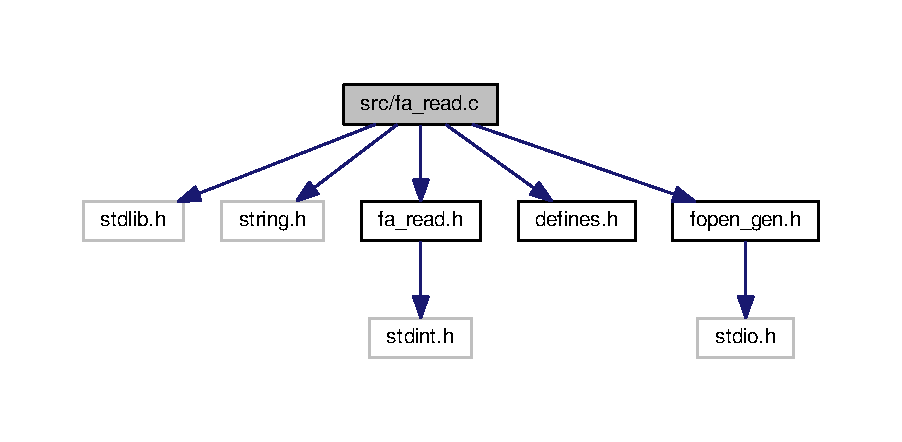
\includegraphics[width=350pt]{fa__read_8c__incl}
\end{center}
\end{figure}
\subsection*{Functions}
\begin{DoxyCompactItemize}
\item 
static int \hyperlink{fa__read_8c_ac5288f4a36dea040a40048bebb21ba34}{ignore\+\_\+line} (char $\ast$line)
\begin{DoxyCompactList}\small\item\em ignore header lines. \end{DoxyCompactList}\item 
static void \hyperlink{fa__read_8c_a5e790c4eb9bfc71776032610a65d88d7}{init\+\_\+fa} (\hyperlink{fa__read_8h_a797328b16bc1c1088998cd164aafb09d}{Fa\+\_\+data} $\ast$ptr\+\_\+fa)
\begin{DoxyCompactList}\small\item\em Initialization of Fa\+\_\+data. \end{DoxyCompactList}\item 
static void \hyperlink{fa__read_8c_a5c08d4c247d5c3e55bb572fb8d6a11bd}{realloc\+\_\+fa} (\hyperlink{fa__read_8h_a797328b16bc1c1088998cd164aafb09d}{Fa\+\_\+data} $\ast$ptr\+\_\+fa)
\begin{DoxyCompactList}\small\item\em Reallocation of Fa\+\_\+data, in case the length of entrylen is exhausted. \end{DoxyCompactList}\item 
static void \hyperlink{fa__read_8c_a58dddba8afcef6229172d7e5e11d6d77}{init\+\_\+entries} (\hyperlink{fa__read_8h_a797328b16bc1c1088998cd164aafb09d}{Fa\+\_\+data} $\ast$ptr\+\_\+fa)
\begin{DoxyCompactList}\small\item\em Allocation of Fa\+\_\+entries. \end{DoxyCompactList}\item 
static uint64\+\_\+t \hyperlink{fa__read_8c_aa1d4ac6800d8769ad1c917299579a81f}{sweep\+\_\+fa} (char $\ast$filename, \hyperlink{fa__read_8h_a797328b16bc1c1088998cd164aafb09d}{Fa\+\_\+data} $\ast$ptr\+\_\+fa)
\begin{DoxyCompactList}\small\item\em this function sweeps a fasta file to obtain structure details. \end{DoxyCompactList}\item 
int \hyperlink{fa__read_8c_a4d2d77d66924fdc762222c8f28f9718a}{read\+\_\+fasta} (char $\ast$filename, \hyperlink{fa__read_8h_a797328b16bc1c1088998cd164aafb09d}{Fa\+\_\+data} $\ast$ptr\+\_\+fa)
\begin{DoxyCompactList}\small\item\em reads a fasta file and stores the contents in a Fa\+\_\+data structure. \end{DoxyCompactList}\item 
uint64\+\_\+t \hyperlink{fa__read_8c_a0e6b9d47a8472d0768270afbdbf17d4e}{size\+\_\+fasta} (\hyperlink{fa__read_8h_a797328b16bc1c1088998cd164aafb09d}{Fa\+\_\+data} $\ast$ptr\+\_\+fa)
\begin{DoxyCompactList}\small\item\em computes length of genome in fasta structure \end{DoxyCompactList}\item 
void \hyperlink{fa__read_8c_a714b70ff332a85349cd52b76965dd444}{free\+\_\+fasta} (\hyperlink{fa__read_8h_a797328b16bc1c1088998cd164aafb09d}{Fa\+\_\+data} $\ast$ptr\+\_\+fa)
\begin{DoxyCompactList}\small\item\em free fasta file \end{DoxyCompactList}\end{DoxyCompactItemize}
\subsection*{Variables}
\begin{DoxyCompactItemize}
\item 
uint64\+\_\+t \hyperlink{fa__read_8c_a1f18264718e0b1b1be5a1f0ee64431e4}{alloc\+\_\+mem}
\end{DoxyCompactItemize}


\subsection{Detailed Description}
reads in and stores fasta files 

\begin{DoxyAuthor}{Author}
Paula Perez \href{mailto:paulaperezrubio@gmail.com}{\tt paulaperezrubio@gmail.\+com} 
\end{DoxyAuthor}
\begin{DoxyDate}{Date}
18.\+08.\+2017 
\end{DoxyDate}


\subsection{Function Documentation}
\hypertarget{fa__read_8c_a714b70ff332a85349cd52b76965dd444}{\index{fa\+\_\+read.\+c@{fa\+\_\+read.\+c}!free\+\_\+fasta@{free\+\_\+fasta}}
\index{free\+\_\+fasta@{free\+\_\+fasta}!fa\+\_\+read.\+c@{fa\+\_\+read.\+c}}
\subsubsection[{free\+\_\+fasta}]{\setlength{\rightskip}{0pt plus 5cm}void free\+\_\+fasta (
\begin{DoxyParamCaption}
\item[{{\bf Fa\+\_\+data} $\ast$}]{ptr\+\_\+fa}
\end{DoxyParamCaption}
)}}\label{fa__read_8c_a714b70ff332a85349cd52b76965dd444}


free fasta file 


\begin{DoxyParams}{Parameters}
{\em ptr\+\_\+fa} & pointer to Fa\+\_\+data structure.\\
\hline
\end{DoxyParams}
The dynamically allocated memory in a Fa\+\_\+data struct is deallocated and counted, so that we can \hypertarget{fa__read_8c_ac5288f4a36dea040a40048bebb21ba34}{\index{fa\+\_\+read.\+c@{fa\+\_\+read.\+c}!ignore\+\_\+line@{ignore\+\_\+line}}
\index{ignore\+\_\+line@{ignore\+\_\+line}!fa\+\_\+read.\+c@{fa\+\_\+read.\+c}}
\subsubsection[{ignore\+\_\+line}]{\setlength{\rightskip}{0pt plus 5cm}static int ignore\+\_\+line (
\begin{DoxyParamCaption}
\item[{char $\ast$}]{line}
\end{DoxyParamCaption}
)\hspace{0.3cm}{\ttfamily [static]}}}\label{fa__read_8c_ac5288f4a36dea040a40048bebb21ba34}


ignore header lines. 


\begin{DoxyParams}{Parameters}
{\em line} & string of characters. \\
\hline
\end{DoxyParams}
\begin{DoxyReturn}{Returns}
number of characters to jump until a ~\newline
 is found. 
\end{DoxyReturn}
\hypertarget{fa__read_8c_a58dddba8afcef6229172d7e5e11d6d77}{\index{fa\+\_\+read.\+c@{fa\+\_\+read.\+c}!init\+\_\+entries@{init\+\_\+entries}}
\index{init\+\_\+entries@{init\+\_\+entries}!fa\+\_\+read.\+c@{fa\+\_\+read.\+c}}
\subsubsection[{init\+\_\+entries}]{\setlength{\rightskip}{0pt plus 5cm}static void init\+\_\+entries (
\begin{DoxyParamCaption}
\item[{{\bf Fa\+\_\+data} $\ast$}]{ptr\+\_\+fa}
\end{DoxyParamCaption}
)\hspace{0.3cm}{\ttfamily [static]}}}\label{fa__read_8c_a58dddba8afcef6229172d7e5e11d6d77}


Allocation of Fa\+\_\+entries. 


\begin{DoxyParams}{Parameters}
{\em ptr\+\_\+fa} & pointer to Fa\+\_\+data structure.\\
\hline
\end{DoxyParams}
When we have sweeped the fasta file once, we can proceed to allocate the memory for the entries (now we have registered their length). \hypertarget{fa__read_8c_a5e790c4eb9bfc71776032610a65d88d7}{\index{fa\+\_\+read.\+c@{fa\+\_\+read.\+c}!init\+\_\+fa@{init\+\_\+fa}}
\index{init\+\_\+fa@{init\+\_\+fa}!fa\+\_\+read.\+c@{fa\+\_\+read.\+c}}
\subsubsection[{init\+\_\+fa}]{\setlength{\rightskip}{0pt plus 5cm}static void init\+\_\+fa (
\begin{DoxyParamCaption}
\item[{{\bf Fa\+\_\+data} $\ast$}]{ptr\+\_\+fa}
\end{DoxyParamCaption}
)\hspace{0.3cm}{\ttfamily [static]}}}\label{fa__read_8c_a5e790c4eb9bfc71776032610a65d88d7}


Initialization of Fa\+\_\+data. 


\begin{DoxyParams}{Parameters}
{\em ptr\+\_\+fa} & pointer to Fa\+\_\+data structure.\\
\hline
\end{DoxyParams}
Initializes nlines, linelen, nentries to 0 and allocates memory for entrylen (F\+A\+\_\+\+E\+N\+T\+R\+Y\+\_\+\+B\+U\+F entries). \hypertarget{fa__read_8c_a4d2d77d66924fdc762222c8f28f9718a}{\index{fa\+\_\+read.\+c@{fa\+\_\+read.\+c}!read\+\_\+fasta@{read\+\_\+fasta}}
\index{read\+\_\+fasta@{read\+\_\+fasta}!fa\+\_\+read.\+c@{fa\+\_\+read.\+c}}
\subsubsection[{read\+\_\+fasta}]{\setlength{\rightskip}{0pt plus 5cm}int read\+\_\+fasta (
\begin{DoxyParamCaption}
\item[{char $\ast$}]{filename, }
\item[{{\bf Fa\+\_\+data} $\ast$}]{ptr\+\_\+fa}
\end{DoxyParamCaption}
)}}\label{fa__read_8c_a4d2d77d66924fdc762222c8f28f9718a}


reads a fasta file and stores the contents in a Fa\+\_\+data structure. 


\begin{DoxyParams}{Parameters}
{\em filename} & path to a fasta input file. \\
\hline
{\em ptr\+\_\+fa} & pointer to Fa\+\_\+data structure. \\
\hline
\end{DoxyParams}
\begin{DoxyReturn}{Returns}
number of entries in the fasta file.
\end{DoxyReturn}
A fasta file is read and stored in a structure Fa\+\_\+data The basic problem with reading F\+A\+S\+T\+A files is that there is no end-\/of-\/record indicator. When you're reading sequence n, you don't know you're done until you've read the header line for sequence n+1, which you won't parse 'til later (when you're reading in the sequence n+1). The solution implemented here is to read the file twice. The first time, (sweep\+\_\+fa), we initialize Fa\+\_\+data and store the parameters\+:
\begin{DoxyItemize}
\item nlines\+: number of lines of the fasta file.
\item nentries\+: number of entries in the fasta file.
\item linelen\+: length of a line in the considered fasta file.
\item entrylen\+: array containing the lengths of every entry. With this information, the pointer to Fa\+\_\+entry can be allocated and the file is read again and the entries are stored in the structure. 
\end{DoxyItemize}\hypertarget{fa__read_8c_a5c08d4c247d5c3e55bb572fb8d6a11bd}{\index{fa\+\_\+read.\+c@{fa\+\_\+read.\+c}!realloc\+\_\+fa@{realloc\+\_\+fa}}
\index{realloc\+\_\+fa@{realloc\+\_\+fa}!fa\+\_\+read.\+c@{fa\+\_\+read.\+c}}
\subsubsection[{realloc\+\_\+fa}]{\setlength{\rightskip}{0pt plus 5cm}static void realloc\+\_\+fa (
\begin{DoxyParamCaption}
\item[{{\bf Fa\+\_\+data} $\ast$}]{ptr\+\_\+fa}
\end{DoxyParamCaption}
)\hspace{0.3cm}{\ttfamily [static]}}}\label{fa__read_8c_a5c08d4c247d5c3e55bb572fb8d6a11bd}


Reallocation of Fa\+\_\+data, in case the length of entrylen is exhausted. 


\begin{DoxyParams}{Parameters}
{\em ptr\+\_\+fa} & pointer to Fa\+\_\+data structure. \\
\hline
\end{DoxyParams}
\hypertarget{fa__read_8c_a0e6b9d47a8472d0768270afbdbf17d4e}{\index{fa\+\_\+read.\+c@{fa\+\_\+read.\+c}!size\+\_\+fasta@{size\+\_\+fasta}}
\index{size\+\_\+fasta@{size\+\_\+fasta}!fa\+\_\+read.\+c@{fa\+\_\+read.\+c}}
\subsubsection[{size\+\_\+fasta}]{\setlength{\rightskip}{0pt plus 5cm}uint64\+\_\+t size\+\_\+fasta (
\begin{DoxyParamCaption}
\item[{{\bf Fa\+\_\+data} $\ast$}]{ptr\+\_\+fa}
\end{DoxyParamCaption}
)}}\label{fa__read_8c_a0e6b9d47a8472d0768270afbdbf17d4e}


computes length of genome in fasta structure 


\begin{DoxyParams}{Parameters}
{\em ptr\+\_\+fa} & pointer to Fa\+\_\+data \\
\hline
\end{DoxyParams}
\begin{DoxyReturn}{Returns}
total number of nucleotides 
\end{DoxyReturn}
\hypertarget{fa__read_8c_aa1d4ac6800d8769ad1c917299579a81f}{\index{fa\+\_\+read.\+c@{fa\+\_\+read.\+c}!sweep\+\_\+fa@{sweep\+\_\+fa}}
\index{sweep\+\_\+fa@{sweep\+\_\+fa}!fa\+\_\+read.\+c@{fa\+\_\+read.\+c}}
\subsubsection[{sweep\+\_\+fa}]{\setlength{\rightskip}{0pt plus 5cm}static uint64\+\_\+t sweep\+\_\+fa (
\begin{DoxyParamCaption}
\item[{char $\ast$}]{filename, }
\item[{{\bf Fa\+\_\+data} $\ast$}]{ptr\+\_\+fa}
\end{DoxyParamCaption}
)\hspace{0.3cm}{\ttfamily [static]}}}\label{fa__read_8c_aa1d4ac6800d8769ad1c917299579a81f}


this function sweeps a fasta file to obtain structure details. 


\begin{DoxyParams}{Parameters}
{\em filename} & path to a fasta input file. \\
\hline
{\em ptr\+\_\+fa} & pointer to Fa\+\_\+data structure. \\
\hline
\end{DoxyParams}
\begin{DoxyReturn}{Returns}
size of fasta file.
\end{DoxyReturn}
This function sweeps over the fasta file once to annotate how many entries there are, how long they are, how many characters there are per line, and how many lines the file has. 

\subsection{Variable Documentation}
\hypertarget{fa__read_8c_a1f18264718e0b1b1be5a1f0ee64431e4}{\index{fa\+\_\+read.\+c@{fa\+\_\+read.\+c}!alloc\+\_\+mem@{alloc\+\_\+mem}}
\index{alloc\+\_\+mem@{alloc\+\_\+mem}!fa\+\_\+read.\+c@{fa\+\_\+read.\+c}}
\subsubsection[{alloc\+\_\+mem}]{\setlength{\rightskip}{0pt plus 5cm}uint64\+\_\+t alloc\+\_\+mem}}\label{fa__read_8c_a1f18264718e0b1b1be5a1f0ee64431e4}
global variable. Memory allocated in the heap. 
\hypertarget{fopen__gen_8c}{}\section{src/fopen\+\_\+gen.c File Reference}
\label{fopen__gen_8c}\index{src/fopen\+\_\+gen.\+c@{src/fopen\+\_\+gen.\+c}}


Uncompress/compress input/output files using pipes.  


{\ttfamily \#include $<$stdlib.\+h$>$}\newline
{\ttfamily \#include $<$string.\+h$>$}\newline
{\ttfamily \#include $<$unistd.\+h$>$}\newline
{\ttfamily \#include $<$assert.\+h$>$}\newline
{\ttfamily \#include $<$sys/types.\+h$>$}\newline
{\ttfamily \#include $<$fcntl.\+h$>$}\newline
{\ttfamily \#include \char`\"{}fopen\+\_\+gen.\+h\char`\"{}}\newline
Include dependency graph for fopen\+\_\+gen.\+c\+:
\nopagebreak
\begin{figure}[H]
\begin{center}
\leavevmode
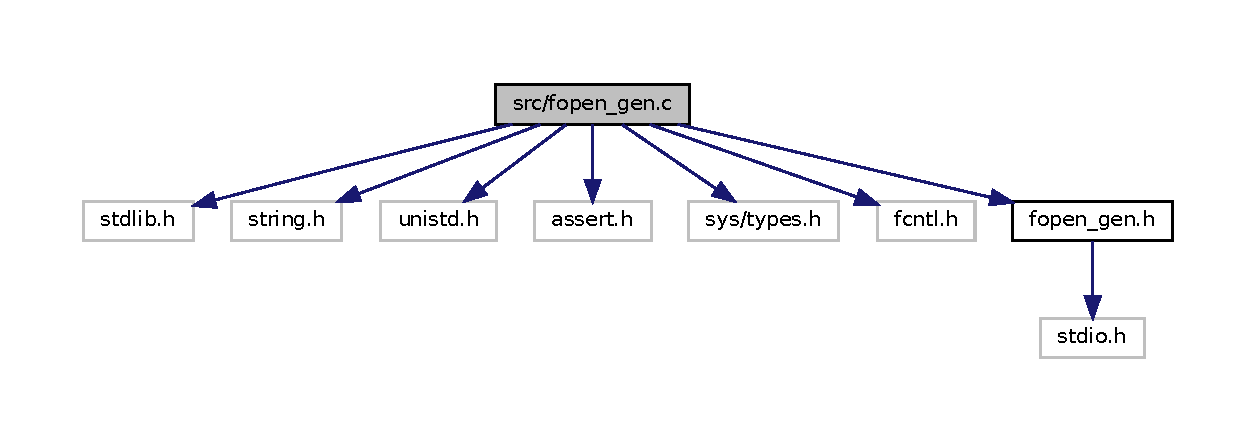
\includegraphics[width=350pt]{fopen__gen_8c__incl}
\end{center}
\end{figure}
\subsection*{Functions}
\begin{DoxyCompactItemize}
\item 
\mbox{\Hypertarget{fopen__gen_8c_a103afa931e1ef96c23ac490151b64036}\label{fopen__gen_8c_a103afa931e1ef96c23ac490151b64036}} 
static const char $\ast$ {\bfseries zcat\+Exec} (const char $\ast$path)
\item 
\mbox{\Hypertarget{fopen__gen_8c_aaad17dde0a82955fa873b2a8b93c99ae}\label{fopen__gen_8c_aaad17dde0a82955fa873b2a8b93c99ae}} 
static const char $\ast$ \mbox{\hyperlink{fopen__gen_8c_aaad17dde0a82955fa873b2a8b93c99ae}{cat\+Exec}} (const char $\ast$path)
\begin{DoxyCompactList}\small\item\em Commands to compress files. To be done in output. \end{DoxyCompactList}\item 
static int \mbox{\hyperlink{fopen__gen_8c_ad91f7120fe65477ca4ccc599808434e6}{uncompress}} (const char $\ast$path)
\begin{DoxyCompactList}\small\item\em Open a pipe to uncompress file. Open a pipe to uncompress the specified file. Not thread safe. \end{DoxyCompactList}\item 
static int \mbox{\hyperlink{fopen__gen_8c_a1d546df97e4f524a9a23e4e5bb92cff9}{compress}} (const char $\ast$path)
\begin{DoxyCompactList}\small\item\em Open a pipe to compress output. Open a pipe to uncompress the specified file. Not thread safe. \end{DoxyCompactList}\item 
\mbox{\Hypertarget{fopen__gen_8c_ae59755703d84f781f127762acf2deb6d}\label{fopen__gen_8c_ae59755703d84f781f127762acf2deb6d}} 
int {\bfseries set\+Cloexec} (int fd)
\item 
static F\+I\+LE $\ast$ \mbox{\hyperlink{fopen__gen_8c_a97fe7a7fd381b9f81e4adbdeab902766}{funcompress}} (const char $\ast$path)
\begin{DoxyCompactList}\small\item\em Open a pipe to uncompress the specified file. \end{DoxyCompactList}\item 
static F\+I\+LE $\ast$ \mbox{\hyperlink{fopen__gen_8c_a86f9e75b840d00dce91e44cf880f730d}{fcompress}} (const char $\ast$path)
\begin{DoxyCompactList}\small\item\em Open a pipe to compress the specified file. \end{DoxyCompactList}\item 
F\+I\+LE $\ast$ \mbox{\hyperlink{fopen__gen_8c_ae03fc1b9180f740dcb577fdb00072fb3}{fopen\+\_\+gen}} (const char $\ast$path, const char $\ast$mode)
\begin{DoxyCompactList}\small\item\em Generalized fopen function. fopen\+\_\+gen is to be used as fopen. Can be used in read and in write mode. When used in read mode with a compressed extension, the file will be first decompressed and then read. When used in write mode with a compressed extension, the output will be compressed. \end{DoxyCompactList}\end{DoxyCompactItemize}


\subsection{Detailed Description}
Uncompress/compress input/output files using pipes. 

Hook the standard file opening functions, open, fopen and fopen64. If the extension of the file being opened indicates the file is compressed (.gz, .bz2, .xz), when opening in the reading mode a pipe to a program is opened that decompresses that file (gunzip, bunzip2 or xzdec) and return a handle to the open pipe. When opening in the writing mode (only for .gz, .bam), a pipe to a program is opened that compresses the output.

\begin{DoxyAuthor}{Author}
Paula Perez \href{mailto:paulaperezrubio@gmail.com}{\tt paulaperezrubio@gmail.\+com} 
\end{DoxyAuthor}
\begin{DoxyDate}{Date}
03.\+08.\+2017 
\end{DoxyDate}
\begin{DoxyWarning}{Warning}
vfork vs fork to be checked! 
\end{DoxyWarning}
\begin{DoxyNote}{Note}
-\/ original copyright note -\/ (reading mode, original C++ code) author\+: Shaun Jackman \href{mailto:sjackman@bcgsc.ca}{\tt sjackman@bcgsc.\+ca}, \href{https://github.com/bcgsc,}{\tt https\+://github.\+com/bcgsc,} ~\newline
filename\+: Uncompress.\+cpp 
\end{DoxyNote}


\subsection{Function Documentation}
\mbox{\Hypertarget{fopen__gen_8c_a1d546df97e4f524a9a23e4e5bb92cff9}\label{fopen__gen_8c_a1d546df97e4f524a9a23e4e5bb92cff9}} 
\index{fopen\+\_\+gen.\+c@{fopen\+\_\+gen.\+c}!compress@{compress}}
\index{compress@{compress}!fopen\+\_\+gen.\+c@{fopen\+\_\+gen.\+c}}
\subsubsection{\texorpdfstring{compress()}{compress()}}
{\footnotesize\ttfamily static int compress (\begin{DoxyParamCaption}\item[{const char $\ast$}]{path }\end{DoxyParamCaption})\hspace{0.3cm}{\ttfamily [static]}}



Open a pipe to compress output. Open a pipe to uncompress the specified file. Not thread safe. 

\begin{DoxyReturn}{Returns}
a file descriptor 
\end{DoxyReturn}
\mbox{\Hypertarget{fopen__gen_8c_a86f9e75b840d00dce91e44cf880f730d}\label{fopen__gen_8c_a86f9e75b840d00dce91e44cf880f730d}} 
\index{fopen\+\_\+gen.\+c@{fopen\+\_\+gen.\+c}!fcompress@{fcompress}}
\index{fcompress@{fcompress}!fopen\+\_\+gen.\+c@{fopen\+\_\+gen.\+c}}
\subsubsection{\texorpdfstring{fcompress()}{fcompress()}}
{\footnotesize\ttfamily static F\+I\+LE$\ast$ fcompress (\begin{DoxyParamCaption}\item[{const char $\ast$}]{path }\end{DoxyParamCaption})\hspace{0.3cm}{\ttfamily [static]}}



Open a pipe to compress the specified file. 

\begin{DoxyReturn}{Returns}
a F\+I\+LE pointer 
\end{DoxyReturn}
\mbox{\Hypertarget{fopen__gen_8c_ae03fc1b9180f740dcb577fdb00072fb3}\label{fopen__gen_8c_ae03fc1b9180f740dcb577fdb00072fb3}} 
\index{fopen\+\_\+gen.\+c@{fopen\+\_\+gen.\+c}!fopen\+\_\+gen@{fopen\+\_\+gen}}
\index{fopen\+\_\+gen@{fopen\+\_\+gen}!fopen\+\_\+gen.\+c@{fopen\+\_\+gen.\+c}}
\subsubsection{\texorpdfstring{fopen\+\_\+gen()}{fopen\_gen()}}
{\footnotesize\ttfamily F\+I\+LE$\ast$ fopen\+\_\+gen (\begin{DoxyParamCaption}\item[{const char $\ast$}]{path,  }\item[{const char $\ast$}]{mode }\end{DoxyParamCaption})}



Generalized fopen function. fopen\+\_\+gen is to be used as fopen. Can be used in read and in write mode. When used in read mode with a compressed extension, the file will be first decompressed and then read. When used in write mode with a compressed extension, the output will be compressed. 

\begin{DoxyReturn}{Returns}
a F\+I\+LE pointer 
\end{DoxyReturn}
\mbox{\Hypertarget{fopen__gen_8c_a97fe7a7fd381b9f81e4adbdeab902766}\label{fopen__gen_8c_a97fe7a7fd381b9f81e4adbdeab902766}} 
\index{fopen\+\_\+gen.\+c@{fopen\+\_\+gen.\+c}!funcompress@{funcompress}}
\index{funcompress@{funcompress}!fopen\+\_\+gen.\+c@{fopen\+\_\+gen.\+c}}
\subsubsection{\texorpdfstring{funcompress()}{funcompress()}}
{\footnotesize\ttfamily static F\+I\+LE$\ast$ funcompress (\begin{DoxyParamCaption}\item[{const char $\ast$}]{path }\end{DoxyParamCaption})\hspace{0.3cm}{\ttfamily [static]}}



Open a pipe to uncompress the specified file. 

\begin{DoxyReturn}{Returns}
a F\+I\+LE pointer 
\end{DoxyReturn}
\mbox{\Hypertarget{fopen__gen_8c_ad91f7120fe65477ca4ccc599808434e6}\label{fopen__gen_8c_ad91f7120fe65477ca4ccc599808434e6}} 
\index{fopen\+\_\+gen.\+c@{fopen\+\_\+gen.\+c}!uncompress@{uncompress}}
\index{uncompress@{uncompress}!fopen\+\_\+gen.\+c@{fopen\+\_\+gen.\+c}}
\subsubsection{\texorpdfstring{uncompress()}{uncompress()}}
{\footnotesize\ttfamily static int uncompress (\begin{DoxyParamCaption}\item[{const char $\ast$}]{path }\end{DoxyParamCaption})\hspace{0.3cm}{\ttfamily [static]}}



Open a pipe to uncompress file. Open a pipe to uncompress the specified file. Not thread safe. 

\begin{DoxyReturn}{Returns}
a file descriptor 
\end{DoxyReturn}

\hypertarget{fq__read_8c}{\section{src/fq\+\_\+read.c File Reference}
\label{fq__read_8c}\index{src/fq\+\_\+read.\+c@{src/fq\+\_\+read.\+c}}
}


fastq entries manipulations (read/write)  


{\ttfamily \#include $<$string.\+h$>$}\\*
{\ttfamily \#include $<$stdio.\+h$>$}\\*
{\ttfamily \#include $<$stdlib.\+h$>$}\\*
{\ttfamily \#include \char`\"{}init\+\_\+\+Qreport.\+h\char`\"{}}\\*
{\ttfamily \#include \char`\"{}fq\+\_\+read.\+h\char`\"{}}\\*
{\ttfamily \#include \char`\"{}str\+\_\+manip.\+h\char`\"{}}\\*
Include dependency graph for fq\+\_\+read.\+c\+:\nopagebreak
\begin{figure}[H]
\begin{center}
\leavevmode
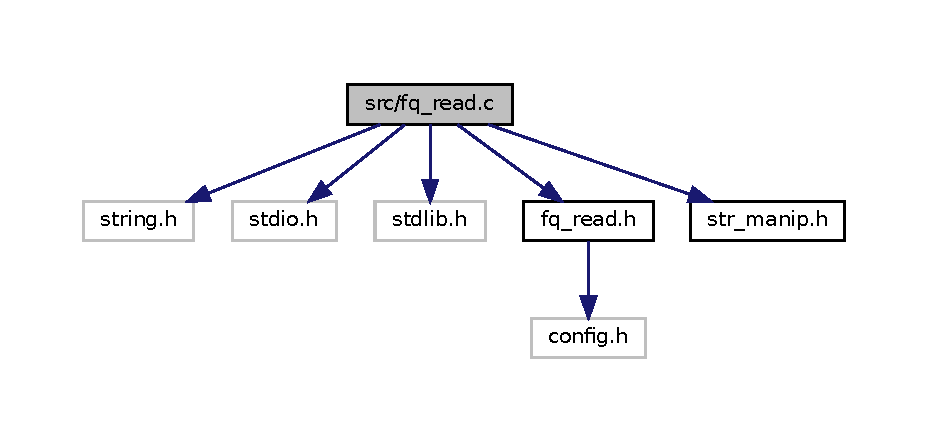
\includegraphics[width=350pt]{fq__read_8c__incl}
\end{center}
\end{figure}
\subsection*{Functions}
\begin{DoxyCompactItemize}
\item 
void \hyperlink{fq__read_8c_a65766fec27771b0b42524625f76d067b}{get\+\_\+fqread} (\hyperlink{fq__read_8h_a9af37aa81397c9531c66863d4e97f034}{Fq\+\_\+read} $\ast$seq, char $\ast$buffer, int pos1, int pos2, int nline)
\begin{DoxyCompactList}\small\item\em reads fastq line from a buffer \end{DoxyCompactList}\item 
int \hyperlink{fq__read_8c_ae58e185777143cd1fc4c75fccd5c647a}{string\+\_\+seq} (\hyperlink{fq__read_8h_a9af37aa81397c9531c66863d4e97f034}{Fq\+\_\+read} $\ast$seq, char $\ast$char\+\_\+seq)
\begin{DoxyCompactList}\small\item\em writes the fq entry in a string \end{DoxyCompactList}\end{DoxyCompactItemize}
\subsection*{Variables}
\begin{DoxyCompactItemize}
\item 
\hyperlink{init__Qreport_8h_a883b1b3db368b84ab55f011bbb41bc80}{Iparam\+\_\+\+Qreport} \hyperlink{fq__read_8c_a5c6527d396580d559cfd1916fc959e23}{par\+\_\+\+Q\+R}
\end{DoxyCompactItemize}


\subsection{Detailed Description}
fastq entries manipulations (read/write) 

\begin{DoxyAuthor}{Author}
Paula Perez \href{mailto:paulaperezrubio@gmail.com}{\tt paulaperezrubio@gmail.\+com} 
\end{DoxyAuthor}
\begin{DoxyDate}{Date}
03.\+08.\+2017 
\end{DoxyDate}


\subsection{Function Documentation}
\hypertarget{fq__read_8c_a65766fec27771b0b42524625f76d067b}{\index{fq\+\_\+read.\+c@{fq\+\_\+read.\+c}!get\+\_\+fqread@{get\+\_\+fqread}}
\index{get\+\_\+fqread@{get\+\_\+fqread}!fq\+\_\+read.\+c@{fq\+\_\+read.\+c}}
\subsubsection[{get\+\_\+fqread}]{\setlength{\rightskip}{0pt plus 5cm}void get\+\_\+fqread (
\begin{DoxyParamCaption}
\item[{{\bf Fq\+\_\+read} $\ast$}]{seq, }
\item[{char $\ast$}]{buffer, }
\item[{int}]{pos1, }
\item[{int}]{pos2, }
\item[{int}]{nline}
\end{DoxyParamCaption}
)}}\label{fq__read_8c_a65766fec27771b0b42524625f76d067b}


reads fastq line from a buffer 

a fastq line is read from a buffer and the relevant information is stored in a structure {\bfseries Fq\+\_\+read}. Depending on the variable {\bfseries par\+\_\+\+Q\+R} values, information about whether the read was trimmed is stored.


\begin{DoxyParams}{Parameters}
{\em $\ast$seq} & pointer to {\bfseries Fq\+\_\+read}, where the info will be stored. \\
\hline
{\em buffer} & variable where the file being read is stored. \\
\hline
{\em pos1} & buffer start position of the line. \\
\hline
{\em pos2} & buffer end position of the line. \\
\hline
{\em nline} & file line number being read. \\
\hline
\end{DoxyParams}
\hypertarget{fq__read_8c_ae58e185777143cd1fc4c75fccd5c647a}{\index{fq\+\_\+read.\+c@{fq\+\_\+read.\+c}!string\+\_\+seq@{string\+\_\+seq}}
\index{string\+\_\+seq@{string\+\_\+seq}!fq\+\_\+read.\+c@{fq\+\_\+read.\+c}}
\subsubsection[{string\+\_\+seq}]{\setlength{\rightskip}{0pt plus 5cm}int string\+\_\+seq (
\begin{DoxyParamCaption}
\item[{{\bf Fq\+\_\+read} $\ast$}]{seq, }
\item[{char $\ast$}]{char\+\_\+seq}
\end{DoxyParamCaption}
)}}\label{fq__read_8c_ae58e185777143cd1fc4c75fccd5c647a}


writes the fq entry in a string 


\begin{DoxyParams}{Parameters}
{\em $\ast$seq} & pointer to {\bfseries Fq\+\_\+read}, where the info will be stored. \\
\hline
{\em char\+\_\+seq} & pointer to buffer, where the sequence will be stored \\
\hline
\end{DoxyParams}
\begin{DoxyWarning}{Warning}
change the call to sprintf to snprintf 
\end{DoxyWarning}


\subsection{Variable Documentation}
\hypertarget{fq__read_8c_a5c6527d396580d559cfd1916fc959e23}{\index{fq\+\_\+read.\+c@{fq\+\_\+read.\+c}!par\+\_\+\+Q\+R@{par\+\_\+\+Q\+R}}
\index{par\+\_\+\+Q\+R@{par\+\_\+\+Q\+R}!fq\+\_\+read.\+c@{fq\+\_\+read.\+c}}
\subsubsection[{par\+\_\+\+Q\+R}]{\setlength{\rightskip}{0pt plus 5cm}{\bf Iparam\+\_\+\+Qreport} par\+\_\+\+Q\+R}}\label{fq__read_8c_a5c6527d396580d559cfd1916fc959e23}
input parameters

global variable\+: input parameters for Qreport 
\hypertarget{init__makeTree_8c}{}\section{src/init\+\_\+make\+Tree.c File Reference}
\label{init__makeTree_8c}\index{src/init\+\_\+make\+Tree.\+c@{src/init\+\_\+make\+Tree.\+c}}


Help dialog for make\+Tree and initialization of the command line arguments.  


{\ttfamily \#include $<$getopt.\+h$>$}\newline
{\ttfamily \#include $<$stdio.\+h$>$}\newline
{\ttfamily \#include $<$stdlib.\+h$>$}\newline
{\ttfamily \#include $<$string.\+h$>$}\newline
{\ttfamily \#include \char`\"{}init\+\_\+make\+Tree.\+h\char`\"{}}\newline
{\ttfamily \#include \char`\"{}str\+\_\+manip.\+h\char`\"{}}\newline
{\ttfamily \#include \char`\"{}config.\+h\char`\"{}}\newline
Include dependency graph for init\+\_\+make\+Tree.\+c\+:
\nopagebreak
\begin{figure}[H]
\begin{center}
\leavevmode
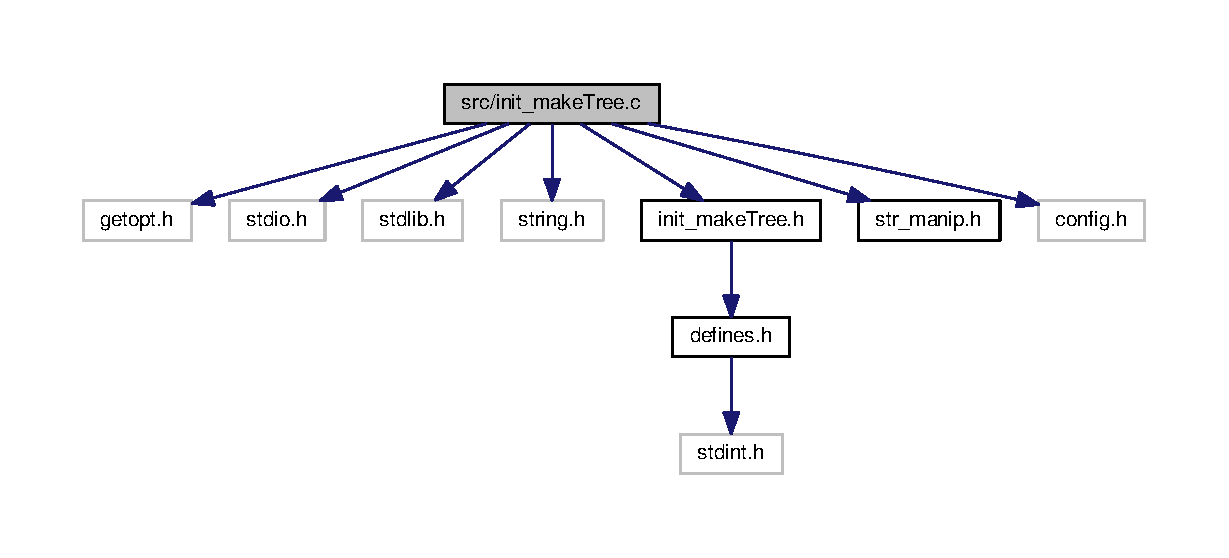
\includegraphics[width=350pt]{init__makeTree_8c__incl}
\end{center}
\end{figure}
\subsection*{Functions}
\begin{DoxyCompactItemize}
\item 
\mbox{\Hypertarget{init__makeTree_8c_a51fb8fb2c64bc9dca004b0e0ecb3997a}\label{init__makeTree_8c_a51fb8fb2c64bc9dca004b0e0ecb3997a}} 
void \mbox{\hyperlink{init__makeTree_8c_a51fb8fb2c64bc9dca004b0e0ecb3997a}{print\+Help\+Dialog\+\_\+make\+Tree}} ()
\begin{DoxyCompactList}\small\item\em Function that prints make\+Tree help dialog when called. \end{DoxyCompactList}\item 
\mbox{\Hypertarget{init__makeTree_8c_a175c3eda9f2120856c04f9bbf4b1bdad}\label{init__makeTree_8c_a175c3eda9f2120856c04f9bbf4b1bdad}} 
void \mbox{\hyperlink{init__makeTree_8c_a175c3eda9f2120856c04f9bbf4b1bdad}{getarg\+\_\+make\+Tree}} (int argc, char $\ast$$\ast$argv)
\begin{DoxyCompactList}\small\item\em Reads in the arguments passed through the command line to make\+Tree. and stores them in the global variable par\+\_\+\+MT. \end{DoxyCompactList}\end{DoxyCompactItemize}
\subsection*{Variables}
\begin{DoxyCompactItemize}
\item 
\mbox{\hyperlink{init__makeTree_8h_a10d824f48589000a94c210c64f08c9a9}{Iparam\+\_\+make\+Tree}} \mbox{\hyperlink{init__makeTree_8c_ad02dd84d6aa8a100953e0c8683c44b7d}{par\+\_\+\+MT}}
\end{DoxyCompactItemize}


\subsection{Detailed Description}
Help dialog for make\+Tree and initialization of the command line arguments. 

\begin{DoxyAuthor}{Author}
Paula Perez \href{mailto:paulaperezrubio@gmail.com}{\tt paulaperezrubio@gmail.\+com} 
\end{DoxyAuthor}
\begin{DoxyDate}{Date}
23.\+08.\+2017 
\end{DoxyDate}


\subsection{Variable Documentation}
\mbox{\Hypertarget{init__makeTree_8c_ad02dd84d6aa8a100953e0c8683c44b7d}\label{init__makeTree_8c_ad02dd84d6aa8a100953e0c8683c44b7d}} 
\index{init\+\_\+make\+Tree.\+c@{init\+\_\+make\+Tree.\+c}!par\+\_\+\+MT@{par\+\_\+\+MT}}
\index{par\+\_\+\+MT@{par\+\_\+\+MT}!init\+\_\+make\+Tree.\+c@{init\+\_\+make\+Tree.\+c}}
\subsubsection{\texorpdfstring{par\+\_\+\+MT}{par\_MT}}
{\footnotesize\ttfamily \mbox{\hyperlink{init__makeTree_8h_a10d824f48589000a94c210c64f08c9a9}{Iparam\+\_\+make\+Tree}} par\+\_\+\+MT}

Input parameters of make\+Tree

global variable\+: Input parameters of make\+Tree. 
\hypertarget{init__Qreport_8c}{\section{src/init\+\_\+\+Qreport.c File Reference}
\label{init__Qreport_8c}\index{src/init\+\_\+\+Qreport.\+c@{src/init\+\_\+\+Qreport.\+c}}
}


Help dialog for Qreport and initialization of the command line arguments.  


{\ttfamily \#include $<$getopt.\+h$>$}\\*
{\ttfamily \#include $<$stdio.\+h$>$}\\*
{\ttfamily \#include $<$string.\+h$>$}\\*
{\ttfamily \#include $<$stdlib.\+h$>$}\\*
{\ttfamily \#include \char`\"{}init\+\_\+\+Qreport.\+h\char`\"{}}\\*
{\ttfamily \#include \char`\"{}config.\+h\char`\"{}}\\*
{\ttfamily \#include \char`\"{}defines.\+h\char`\"{}}\\*
Include dependency graph for init\+\_\+\+Qreport.\+c\+:\nopagebreak
\begin{figure}[H]
\begin{center}
\leavevmode
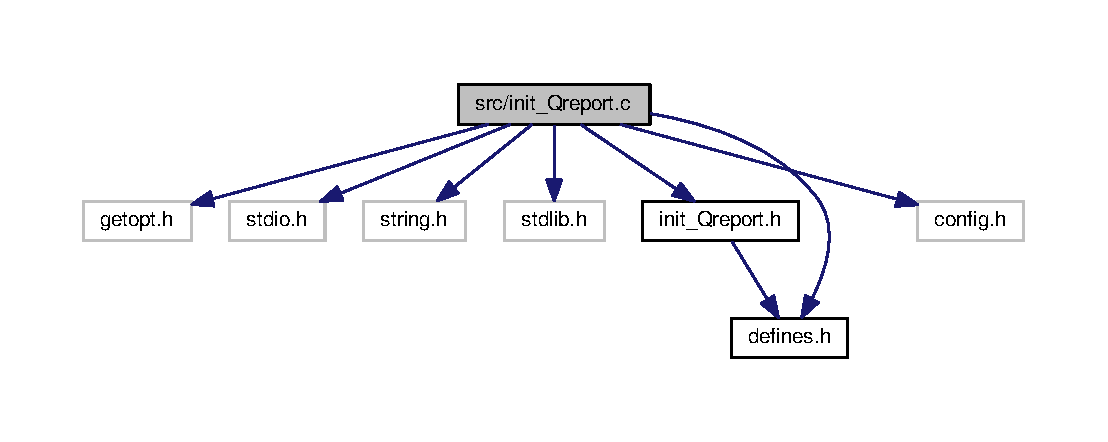
\includegraphics[width=350pt]{init__Qreport_8c__incl}
\end{center}
\end{figure}
\subsection*{Functions}
\begin{DoxyCompactItemize}
\item 
\hypertarget{init__Qreport_8c_a48be775a109c8bf8672933494d67f30f}{void \hyperlink{init__Qreport_8c_a48be775a109c8bf8672933494d67f30f}{print\+Help\+Dialog\+\_\+\+Qreport} ()}\label{init__Qreport_8c_a48be775a109c8bf8672933494d67f30f}

\begin{DoxyCompactList}\small\item\em Function that prints Qreport help dialog when called. \end{DoxyCompactList}\item 
\hypertarget{init__Qreport_8c_a0eb2d9339158f29ffe7ae419af56e921}{void \hyperlink{init__Qreport_8c_a0eb2d9339158f29ffe7ae419af56e921}{getarg\+\_\+\+Qreport} (int argc, char $\ast$$\ast$argv)}\label{init__Qreport_8c_a0eb2d9339158f29ffe7ae419af56e921}

\begin{DoxyCompactList}\small\item\em Reads in the arguments passed through the command line to Qreport. and stores them in the global variable par\+\_\+\+Q\+R. \end{DoxyCompactList}\end{DoxyCompactItemize}
\subsection*{Variables}
\begin{DoxyCompactItemize}
\item 
\hyperlink{init__Qreport_8h_a883b1b3db368b84ab55f011bbb41bc80}{Iparam\+\_\+\+Qreport} \hyperlink{init__Qreport_8c_a5c6527d396580d559cfd1916fc959e23}{par\+\_\+\+Q\+R}
\end{DoxyCompactItemize}


\subsection{Detailed Description}
Help dialog for Qreport and initialization of the command line arguments. 

\begin{DoxyAuthor}{Author}
Paula Perez \href{mailto:paulaperezrubio@gmail.com}{\tt paulaperezrubio@gmail.\+com} 
\end{DoxyAuthor}
\begin{DoxyDate}{Date}
03.\+08.\+2017 
\end{DoxyDate}


\subsection{Variable Documentation}
\hypertarget{init__Qreport_8c_a5c6527d396580d559cfd1916fc959e23}{\index{init\+\_\+\+Qreport.\+c@{init\+\_\+\+Qreport.\+c}!par\+\_\+\+Q\+R@{par\+\_\+\+Q\+R}}
\index{par\+\_\+\+Q\+R@{par\+\_\+\+Q\+R}!init\+\_\+\+Qreport.\+c@{init\+\_\+\+Qreport.\+c}}
\subsubsection[{par\+\_\+\+Q\+R}]{\setlength{\rightskip}{0pt plus 5cm}{\bf Iparam\+\_\+\+Qreport} par\+\_\+\+Q\+R}}\label{init__Qreport_8c_a5c6527d396580d559cfd1916fc959e23}
input parameters

global variable\+: input parameters 
\hypertarget{init__Sreport_8c}{}\section{src/init\+\_\+\+Sreport.c File Reference}
\label{init__Sreport_8c}\index{src/init\+\_\+\+Sreport.\+c@{src/init\+\_\+\+Sreport.\+c}}


Help dialog for Sreport and initialization of the command line arguments.  


{\ttfamily \#include $<$getopt.\+h$>$}\newline
{\ttfamily \#include $<$stdio.\+h$>$}\newline
{\ttfamily \#include $<$stdlib.\+h$>$}\newline
{\ttfamily \#include $<$string.\+h$>$}\newline
{\ttfamily \#include \char`\"{}str\+\_\+manip.\+h\char`\"{}}\newline
{\ttfamily \#include \char`\"{}init\+\_\+\+Sreport.\+h\char`\"{}}\newline
{\ttfamily \#include \char`\"{}config.\+h\char`\"{}}\newline
Include dependency graph for init\+\_\+\+Sreport.\+c\+:
\nopagebreak
\begin{figure}[H]
\begin{center}
\leavevmode
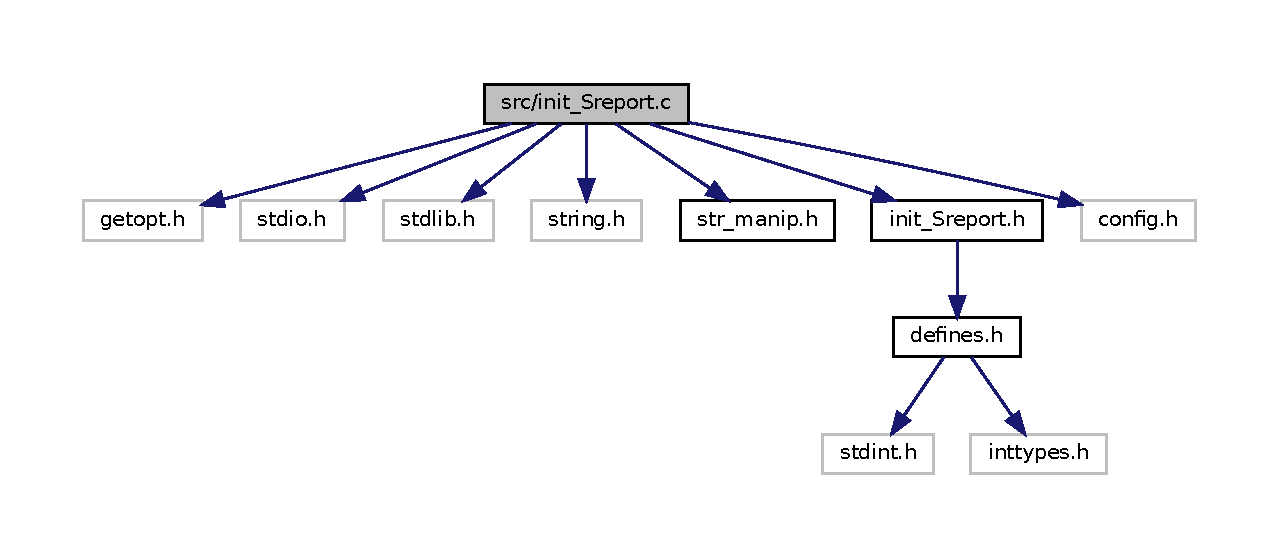
\includegraphics[width=350pt]{init__Sreport_8c__incl}
\end{center}
\end{figure}
\subsection*{Functions}
\begin{DoxyCompactItemize}
\item 
\mbox{\Hypertarget{init__Sreport_8c_a80638b0730feac5c7634c29c6f08ee9e}\label{init__Sreport_8c_a80638b0730feac5c7634c29c6f08ee9e}} 
void \mbox{\hyperlink{init__Sreport_8c_a80638b0730feac5c7634c29c6f08ee9e}{print\+Help\+Dialog\+\_\+\+Sreport}} ()
\begin{DoxyCompactList}\small\item\em Function that prints Sreport help dialog when called. \end{DoxyCompactList}\item 
\mbox{\Hypertarget{init__Sreport_8c_a5a266a01d36227a9094c023aed7a1e8c}\label{init__Sreport_8c_a5a266a01d36227a9094c023aed7a1e8c}} 
void \mbox{\hyperlink{init__Sreport_8c_a5a266a01d36227a9094c023aed7a1e8c}{getarg\+\_\+\+Sreport}} (int argc, char $\ast$$\ast$argv)
\begin{DoxyCompactList}\small\item\em Reads in the arguments passed through the command line to Sreport. and stores them in the global variable par\+\_\+\+SR. \end{DoxyCompactList}\end{DoxyCompactItemize}
\subsection*{Variables}
\begin{DoxyCompactItemize}
\item 
\mbox{\hyperlink{init__Sreport_8h_ae7c35fd710a54db5b21f5c6b04fe9a5d}{Iparam\+\_\+\+Sreport}} \mbox{\hyperlink{init__Sreport_8c_aa230276b7e03d43430c998def780682e}{par\+\_\+\+SR}}
\end{DoxyCompactItemize}


\subsection{Detailed Description}
Help dialog for Sreport and initialization of the command line arguments. 

\begin{DoxyAuthor}{Author}
Paula Perez \href{mailto:paulaperezrubio@gmail.com}{\tt paulaperezrubio@gmail.\+com} 
\end{DoxyAuthor}
\begin{DoxyDate}{Date}
09.\+08.\+2017 
\end{DoxyDate}


\subsection{Variable Documentation}
\mbox{\Hypertarget{init__Sreport_8c_aa230276b7e03d43430c998def780682e}\label{init__Sreport_8c_aa230276b7e03d43430c998def780682e}} 
\index{init\+\_\+\+Sreport.\+c@{init\+\_\+\+Sreport.\+c}!par\+\_\+\+SR@{par\+\_\+\+SR}}
\index{par\+\_\+\+SR@{par\+\_\+\+SR}!init\+\_\+\+Sreport.\+c@{init\+\_\+\+Sreport.\+c}}
\subsubsection{\texorpdfstring{par\+\_\+\+SR}{par\_SR}}
{\footnotesize\ttfamily \mbox{\hyperlink{init__Sreport_8h_ae7c35fd710a54db5b21f5c6b04fe9a5d}{Iparam\+\_\+\+Sreport}} par\+\_\+\+SR}

input parameters Sreport 
\hypertarget{init__trimFilter_8c}{\section{src/init\+\_\+trim\+Filter.c File Reference}
\label{init__trimFilter_8c}\index{src/init\+\_\+trim\+Filter.\+c@{src/init\+\_\+trim\+Filter.\+c}}
}


help dialog for trim\+Filter and initialization of the command line arguments.  


{\ttfamily \#include $<$stdlib.\+h$>$}\\*
{\ttfamily \#include $<$stdio.\+h$>$}\\*
{\ttfamily \#include $<$string.\+h$>$}\\*
{\ttfamily \#include $<$getopt.\+h$>$}\\*
{\ttfamily \#include \char`\"{}init\+\_\+trim\+Filter.\+h\char`\"{}}\\*
{\ttfamily \#include \char`\"{}defines.\+h\char`\"{}}\\*
{\ttfamily \#include \char`\"{}str\+\_\+manip.\+h\char`\"{}}\\*
{\ttfamily \#include \char`\"{}config.\+h\char`\"{}}\\*
Include dependency graph for init\+\_\+trim\+Filter.\+c\+:\nopagebreak
\begin{figure}[H]
\begin{center}
\leavevmode
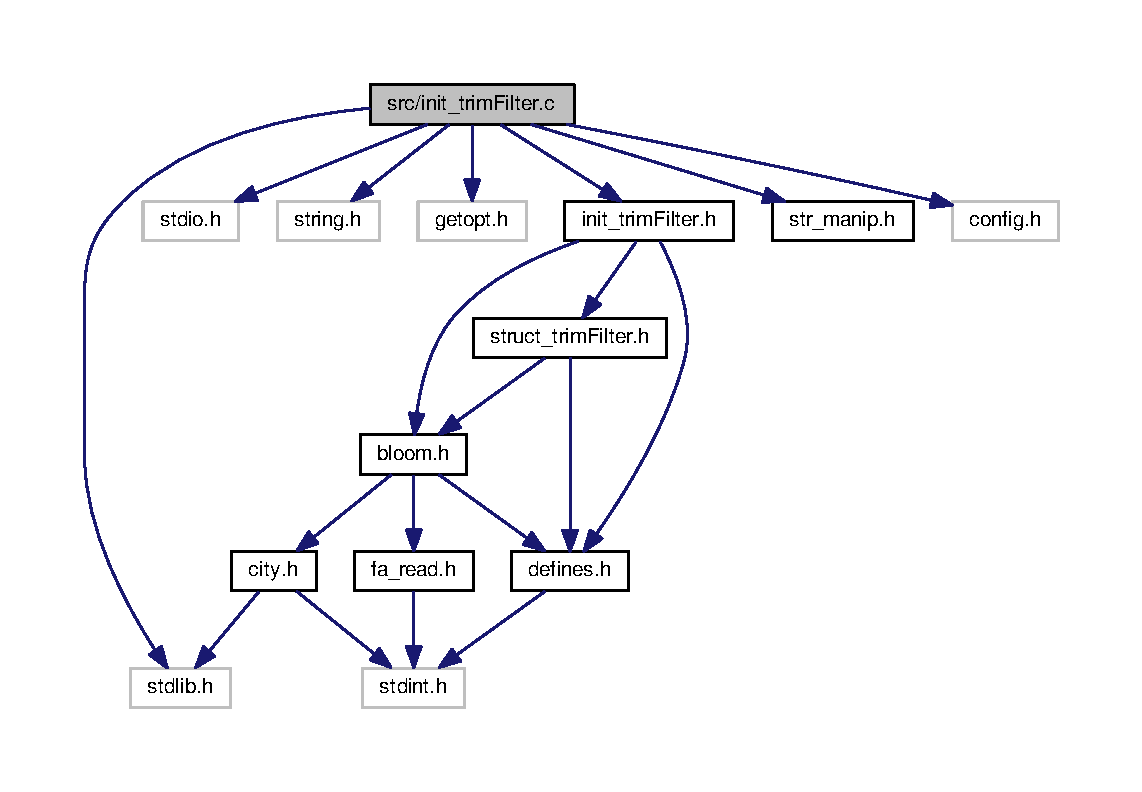
\includegraphics[width=350pt]{init__trimFilter_8c__incl}
\end{center}
\end{figure}
\subsection*{Functions}
\begin{DoxyCompactItemize}
\item 
\hypertarget{init__trimFilter_8c_acb1b66de50f5bfccd87b52851f8de3cc}{void \hyperlink{init__trimFilter_8c_acb1b66de50f5bfccd87b52851f8de3cc}{print\+Help\+Dialog\+\_\+trim\+Filter} ()}\label{init__trimFilter_8c_acb1b66de50f5bfccd87b52851f8de3cc}

\begin{DoxyCompactList}\small\item\em Function that prints trim\+Filter help dialog when called. \end{DoxyCompactList}\item 
\hypertarget{init__trimFilter_8c_a4e5dbdc70417040f72231b5167987b4a}{void \hyperlink{init__trimFilter_8c_a4e5dbdc70417040f72231b5167987b4a}{getarg\+\_\+trim\+Filter} (int argc, char $\ast$$\ast$argv)}\label{init__trimFilter_8c_a4e5dbdc70417040f72231b5167987b4a}

\begin{DoxyCompactList}\small\item\em Reads in the arguments passed through the command line to trim\+Filter. and stores them in the global variable par\+\_\+\+T\+F. \end{DoxyCompactList}\end{DoxyCompactItemize}
\subsection*{Variables}
\begin{DoxyCompactItemize}
\item 
\hyperlink{init__trimFilter_8h_aff83806f1ff2b5f3609dc7d4c04b7c19}{Iparam\+\_\+trim\+Filter} \hyperlink{init__trimFilter_8c_aed14b08f25fd6aa9a6cffb8c0074c953}{par\+\_\+\+T\+F}
\end{DoxyCompactItemize}


\subsection{Detailed Description}
help dialog for trim\+Filter and initialization of the command line arguments. 

\begin{DoxyAuthor}{Author}
Paula Perez \href{mailto:paulaperezrubio@gmail.com}{\tt paulaperezrubio@gmail.\+com} 
\end{DoxyAuthor}
\begin{DoxyDate}{Date}
24.\+08.\+2017 
\end{DoxyDate}


\subsection{Variable Documentation}
\hypertarget{init__trimFilter_8c_aed14b08f25fd6aa9a6cffb8c0074c953}{\index{init\+\_\+trim\+Filter.\+c@{init\+\_\+trim\+Filter.\+c}!par\+\_\+\+T\+F@{par\+\_\+\+T\+F}}
\index{par\+\_\+\+T\+F@{par\+\_\+\+T\+F}!init\+\_\+trim\+Filter.\+c@{init\+\_\+trim\+Filter.\+c}}
\subsubsection[{par\+\_\+\+T\+F}]{\setlength{\rightskip}{0pt plus 5cm}{\bf Iparam\+\_\+trim\+Filter} par\+\_\+\+T\+F}}\label{init__trimFilter_8c_aed14b08f25fd6aa9a6cffb8c0074c953}
Input parameters of make\+Tree

global variable\+: Input parameters of make\+Tree. 
\hypertarget{io__trimFilter_8c}{}\section{src/io\+\_\+trim\+Filter.c File Reference}
\label{io__trimFilter_8c}\index{src/io\+\_\+trim\+Filter.\+c@{src/io\+\_\+trim\+Filter.\+c}}


buffer fq output, write summary file  


{\ttfamily \#include $<$stdio.\+h$>$}\newline
{\ttfamily \#include $<$stdlib.\+h$>$}\newline
{\ttfamily \#include $<$string.\+h$>$}\newline
{\ttfamily \#include \char`\"{}io\+\_\+trim\+Filter.\+h\char`\"{}}\newline
{\ttfamily \#include \char`\"{}defines.\+h\char`\"{}}\newline
Include dependency graph for io\+\_\+trim\+Filter.\+c\+:
\nopagebreak
\begin{figure}[H]
\begin{center}
\leavevmode
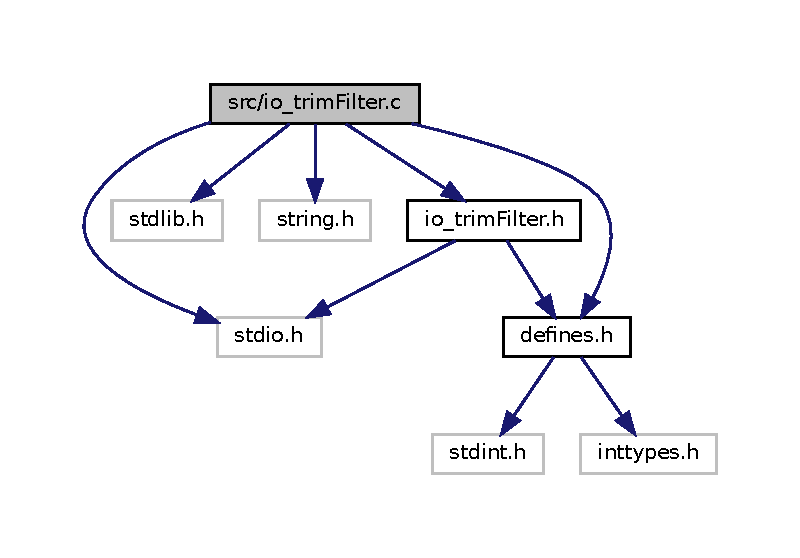
\includegraphics[width=350pt]{io__trimFilter_8c__incl}
\end{center}
\end{figure}
\subsection*{Functions}
\begin{DoxyCompactItemize}
\item 
void \mbox{\hyperlink{io__trimFilter_8c_a9bb3b28738f1a022ccbf4a75bdceea90}{buffer\+\_\+output}} (F\+I\+LE $\ast$fout, const char $\ast$str, const int len, const int fd\+\_\+i)
\begin{DoxyCompactList}\small\item\em buffers the output before writing to disk, writes out summary \end{DoxyCompactList}\item 
\mbox{\Hypertarget{io__trimFilter_8c_a4091d7483c30847a4bea4dabe00c4ffb}\label{io__trimFilter_8c_a4091d7483c30847a4bea4dabe00c4ffb}} 
void \mbox{\hyperlink{io__trimFilter_8c_a4091d7483c30847a4bea4dabe00c4ffb}{write\+\_\+summary\+\_\+\+TF}} (\mbox{\hyperlink{io__trimFilter_8h_a9b921e335cd93e3ad72901eca22b7758}{Stats\+\_\+\+TF}} tf\+\_\+stats, char $\ast$filename)
\begin{DoxyCompactList}\small\item\em writes stats of filtering to summary file (binary) \end{DoxyCompactList}\end{DoxyCompactItemize}


\subsection{Detailed Description}
buffer fq output, write summary file 

\begin{DoxyAuthor}{Author}
Paula Perez \href{mailto:paulaperezrubio@gmail.com}{\tt paulaperezrubio@gmail.\+com} 
\end{DoxyAuthor}
\begin{DoxyDate}{Date}
29.\+08.\+2017 
\end{DoxyDate}


\subsection{Function Documentation}
\mbox{\Hypertarget{io__trimFilter_8c_a9bb3b28738f1a022ccbf4a75bdceea90}\label{io__trimFilter_8c_a9bb3b28738f1a022ccbf4a75bdceea90}} 
\index{io\+\_\+trim\+Filter.\+c@{io\+\_\+trim\+Filter.\+c}!buffer\+\_\+output@{buffer\+\_\+output}}
\index{buffer\+\_\+output@{buffer\+\_\+output}!io\+\_\+trim\+Filter.\+c@{io\+\_\+trim\+Filter.\+c}}
\subsubsection{\texorpdfstring{buffer\+\_\+output()}{buffer\_output()}}
{\footnotesize\ttfamily void buffer\+\_\+output (\begin{DoxyParamCaption}\item[{F\+I\+LE $\ast$}]{fout,  }\item[{const char $\ast$}]{str,  }\item[{const int}]{len,  }\item[{const int}]{fd\+\_\+i }\end{DoxyParamCaption})}



buffers the output before writing to disk, writes out summary 


\begin{DoxyParams}{Parameters}
{\em fout} & F\+I\+LE pointer where we might write to disk; \\
\hline
{\em str} & string we want to add \\
\hline
{\em len} & length of the string we want to add \\
\hline
{\em fd\+\_\+i} & identifier\+: G\+O\+OD, A\+D\+AP, C\+O\+NT, L\+O\+WQ, N\+N\+NN \\
\hline
\end{DoxyParams}

\hypertarget{Lmer_8c}{\section{src/\+Lmer.c File Reference}
\label{Lmer_8c}\index{src/\+Lmer.\+c@{src/\+Lmer.\+c}}
}


Manipulation of Lmers and sequences.  


{\ttfamily \#include \char`\"{}Lmer.\+h\char`\"{}}\\*
{\ttfamily \#include $<$stdio.\+h$>$}\\*
Include dependency graph for Lmer.\+c\+:\nopagebreak
\begin{figure}[H]
\begin{center}
\leavevmode
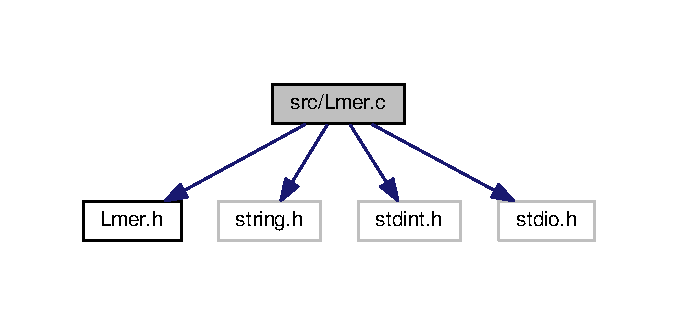
\includegraphics[width=192pt]{Lmer_8c__incl}
\end{center}
\end{figure}
\subsection*{Functions}
\begin{DoxyCompactItemize}
\item 
void \hyperlink{Lmer_8c_a5f1586659681cf692359f7c8c003dd8b}{init\+\_\+map} ()
\begin{DoxyCompactList}\small\item\em Initialize lookup table L\+T. \end{DoxyCompactList}\item 
void \hyperlink{Lmer_8c_a54a9d22589c1235957b6472310280e1d}{init\+\_\+map\+\_\+\+S\+A} ()
\begin{DoxyCompactList}\small\item\em Initialize lookup table L\+T (for S\+A) \end{DoxyCompactList}\item 
\hypertarget{Lmer_8c_a3280d056532aa23523d08dfd52b60b51}{void \hyperlink{Lmer_8c_a3280d056532aa23523d08dfd52b60b51}{Lmer\+\_\+s\+Lmer} (char $\ast$Lmer, int L)}\label{Lmer_8c_a3280d056532aa23523d08dfd52b60b51}

\begin{DoxyCompactList}\small\item\em Transforms an Lmer to the convention stored in the lookup table L\+T. \end{DoxyCompactList}\item 
\hypertarget{Lmer_8c_ae4b4f0b75c0a5784ad66d856aed9d39f}{void \hyperlink{Lmer_8c_ae4b4f0b75c0a5784ad66d856aed9d39f}{rev\+\_\+comp} (char $\ast$s\+Lmer, int L)}\label{Lmer_8c_ae4b4f0b75c0a5784ad66d856aed9d39f}

\begin{DoxyCompactList}\small\item\em Obtains the reverse complement, for \{'\textbackslash{}000','\textbackslash{}001','\textbackslash{}002','\textbackslash{}003'\}. \end{DoxyCompactList}\item 
\hypertarget{Lmer_8c_a6adc3e6b4aa23ade6c889592c50c2963}{void \hyperlink{Lmer_8c_a6adc3e6b4aa23ade6c889592c50c2963}{rev\+\_\+comp2} (char $\ast$s\+Lmer, int L)}\label{Lmer_8c_a6adc3e6b4aa23ade6c889592c50c2963}

\begin{DoxyCompactList}\small\item\em Obtains the reverse complement, for \{'\textbackslash{}001','\textbackslash{}002','\textbackslash{}003','\textbackslash{}004'\}. \end{DoxyCompactList}\end{DoxyCompactItemize}
\subsection*{Variables}
\begin{DoxyCompactItemize}
\item 
char \hyperlink{Lmer_8c_abecb1b17de58b71ea7da6803df2486ae}{L\+T} \mbox{[}256\mbox{]}
\item 
char \hyperlink{Lmer_8c_a09f8263f3577dfabc13a037c32504ad3}{Nencode}
\end{DoxyCompactItemize}


\subsection{Detailed Description}
Manipulation of Lmers and sequences. 

\begin{DoxyAuthor}{Author}
Paula Perez \href{mailto:paulaperezrubio@gmail.com}{\tt paulaperezrubio@gmail.\+com} 
\end{DoxyAuthor}
\begin{DoxyDate}{Date}
18.\+08.\+2017 
\end{DoxyDate}


\subsection{Function Documentation}
\hypertarget{Lmer_8c_a5f1586659681cf692359f7c8c003dd8b}{\index{Lmer.\+c@{Lmer.\+c}!init\+\_\+map@{init\+\_\+map}}
\index{init\+\_\+map@{init\+\_\+map}!Lmer.\+c@{Lmer.\+c}}
\subsubsection[{init\+\_\+map}]{\setlength{\rightskip}{0pt plus 5cm}void init\+\_\+map (
\begin{DoxyParamCaption}
{}
\end{DoxyParamCaption}
)}}\label{Lmer_8c_a5f1586659681cf692359f7c8c003dd8b}


Initialize lookup table L\+T. 

\{'a','c','g','t'\} --$>$ \{'\textbackslash{}000','\textbackslash{}001','\textbackslash{}002','\textbackslash{}003'\}, rest '\textbackslash{}004'. \hypertarget{Lmer_8c_a54a9d22589c1235957b6472310280e1d}{\index{Lmer.\+c@{Lmer.\+c}!init\+\_\+map\+\_\+\+S\+A@{init\+\_\+map\+\_\+\+S\+A}}
\index{init\+\_\+map\+\_\+\+S\+A@{init\+\_\+map\+\_\+\+S\+A}!Lmer.\+c@{Lmer.\+c}}
\subsubsection[{init\+\_\+map\+\_\+\+S\+A}]{\setlength{\rightskip}{0pt plus 5cm}void init\+\_\+map\+\_\+\+S\+A (
\begin{DoxyParamCaption}
{}
\end{DoxyParamCaption}
)}}\label{Lmer_8c_a54a9d22589c1235957b6472310280e1d}


Initialize lookup table L\+T (for S\+A) 

\{'a','c','g','t'\} --$>$ \{'\textbackslash{}001','\textbackslash{}002','\textbackslash{}003','\textbackslash{}004'\}, rest '\textbackslash{}005'. 

\subsection{Variable Documentation}
\hypertarget{Lmer_8c_abecb1b17de58b71ea7da6803df2486ae}{\index{Lmer.\+c@{Lmer.\+c}!L\+T@{L\+T}}
\index{L\+T@{L\+T}!Lmer.\+c@{Lmer.\+c}}
\subsubsection[{L\+T}]{\setlength{\rightskip}{0pt plus 5cm}char L\+T\mbox{[}256\mbox{]}}}\label{Lmer_8c_abecb1b17de58b71ea7da6803df2486ae}
global variable. Lookup table. \hypertarget{Lmer_8c_a09f8263f3577dfabc13a037c32504ad3}{\index{Lmer.\+c@{Lmer.\+c}!Nencode@{Nencode}}
\index{Nencode@{Nencode}!Lmer.\+c@{Lmer.\+c}}
\subsubsection[{Nencode}]{\setlength{\rightskip}{0pt plus 5cm}char Nencode}}\label{Lmer_8c_a09f8263f3577dfabc13a037c32504ad3}
global variable. Encoding for N's(\textbackslash{}004, or \textbackslash{}005) 
\hypertarget{makeTree_8c}{\section{src/make\+Tree.c File Reference}
\label{makeTree_8c}\index{src/make\+Tree.\+c@{src/make\+Tree.\+c}}
}


make\+Tree main function  


{\ttfamily \#include $<$stdlib.\+h$>$}\\*
{\ttfamily \#include $<$stdio.\+h$>$}\\*
{\ttfamily \#include $<$time.\+h$>$}\\*
{\ttfamily \#include \char`\"{}defines.\+h\char`\"{}}\\*
{\ttfamily \#include \char`\"{}fa\+\_\+read.\+h\char`\"{}}\\*
{\ttfamily \#include \char`\"{}tree.\+h\char`\"{}}\\*
{\ttfamily \#include \char`\"{}init\+\_\+make\+Tree.\+h\char`\"{}}\\*
Include dependency graph for make\+Tree.\+c\+:
\nopagebreak
\begin{figure}[H]
\begin{center}
\leavevmode
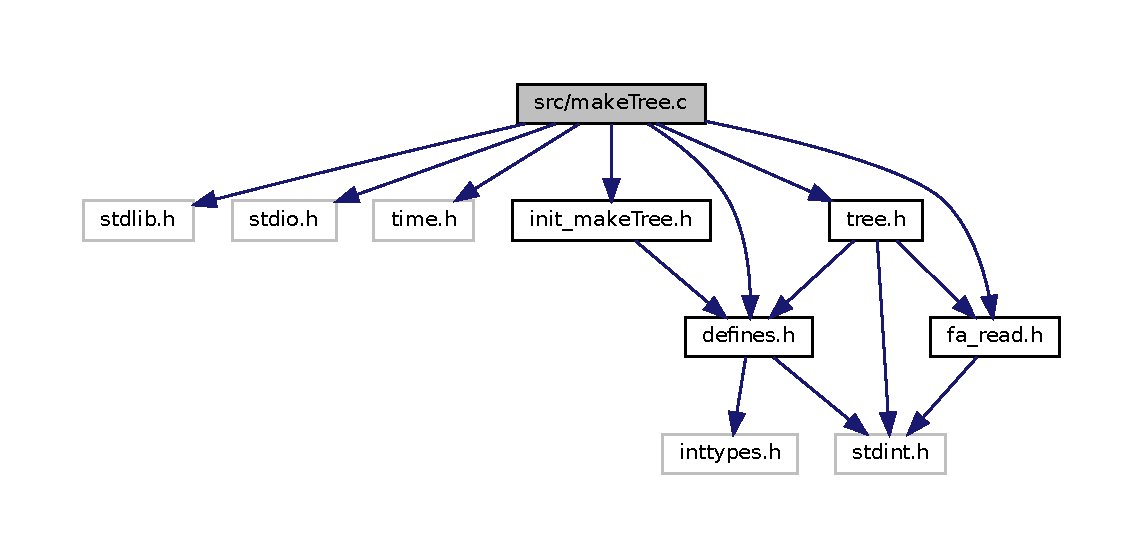
\includegraphics[width=350pt]{makeTree_8c__incl}
\end{center}
\end{figure}
\subsection*{Functions}
\begin{DoxyCompactItemize}
\item 
\hypertarget{makeTree_8c_a0ddf1224851353fc92bfbff6f499fa97}{int \hyperlink{makeTree_8c_a0ddf1224851353fc92bfbff6f499fa97}{main} (int argc, char $\ast$argv\mbox{[}$\,$\mbox{]})}\label{makeTree_8c_a0ddf1224851353fc92bfbff6f499fa97}

\begin{DoxyCompactList}\small\item\em make\+Tree main function \end{DoxyCompactList}\end{DoxyCompactItemize}
\subsection*{Variables}
\begin{DoxyCompactItemize}
\item 
uint64\+\_\+t \hyperlink{makeTree_8c_a1f18264718e0b1b1be5a1f0ee64431e4}{alloc\+\_\+mem} = 0
\item 
\hyperlink{init__makeTree_8h_a10d824f48589000a94c210c64f08c9a9}{Iparam\+\_\+make\+Tree} \hyperlink{makeTree_8c_ad02dd84d6aa8a100953e0c8683c44b7d}{par\+\_\+\+M\+T}
\end{DoxyCompactItemize}


\subsection{Detailed Description}
make\+Tree main function 

\begin{DoxyAuthor}{Author}
Paula Perez \href{mailto:paulaperezrubio@gmail.com}{\tt paulaperezrubio@gmail.\+com} 
\end{DoxyAuthor}
\begin{DoxyDate}{Date}
23.\+08.\+2017 This file contains the make\+Tree main function. It reads a fasta file, constructs a 4-\/tree of depth L and stores it compressed in a file. See R\+E\+A\+D\+M\+E\+\_\+make\+Tree.\+md for more details. 
\end{DoxyDate}


\subsection{Variable Documentation}
\hypertarget{makeTree_8c_a1f18264718e0b1b1be5a1f0ee64431e4}{\index{make\+Tree.\+c@{make\+Tree.\+c}!alloc\+\_\+mem@{alloc\+\_\+mem}}
\index{alloc\+\_\+mem@{alloc\+\_\+mem}!make\+Tree.\+c@{make\+Tree.\+c}}
\subsubsection[{alloc\+\_\+mem}]{\setlength{\rightskip}{0pt plus 5cm}uint64\+\_\+t alloc\+\_\+mem = 0}}\label{makeTree_8c_a1f18264718e0b1b1be5a1f0ee64431e4}
global variable. Memory allocated in the heap. \hypertarget{makeTree_8c_ad02dd84d6aa8a100953e0c8683c44b7d}{\index{make\+Tree.\+c@{make\+Tree.\+c}!par\+\_\+\+M\+T@{par\+\_\+\+M\+T}}
\index{par\+\_\+\+M\+T@{par\+\_\+\+M\+T}!make\+Tree.\+c@{make\+Tree.\+c}}
\subsubsection[{par\+\_\+\+M\+T}]{\setlength{\rightskip}{0pt plus 5cm}{\bf Iparam\+\_\+make\+Tree} par\+\_\+\+M\+T}}\label{makeTree_8c_ad02dd84d6aa8a100953e0c8683c44b7d}
global variable\+: Input parameters of make\+Tree. 
\hypertarget{Qreport_8c}{\section{src/\+Qreport.c File Reference}
\label{Qreport_8c}\index{src/\+Qreport.\+c@{src/\+Qreport.\+c}}
}


Q\+Report main function.  


{\ttfamily \#include $<$stdio.\+h$>$}\\*
{\ttfamily \#include $<$stdlib.\+h$>$}\\*
{\ttfamily \#include $<$string.\+h$>$}\\*
{\ttfamily \#include $<$time.\+h$>$}\\*
{\ttfamily \#include \char`\"{}init\+\_\+\+Qreport.\+h\char`\"{}}\\*
{\ttfamily \#include \char`\"{}fopen\+\_\+gen.\+h\char`\"{}}\\*
{\ttfamily \#include \char`\"{}fq\+\_\+read.\+h\char`\"{}}\\*
{\ttfamily \#include \char`\"{}stats\+\_\+info.\+h\char`\"{}}\\*
{\ttfamily \#include \char`\"{}Rcommand\+\_\+\+Qreport.\+h\char`\"{}}\\*
Include dependency graph for Qreport.\+c\+:
\nopagebreak
\begin{figure}[H]
\begin{center}
\leavevmode
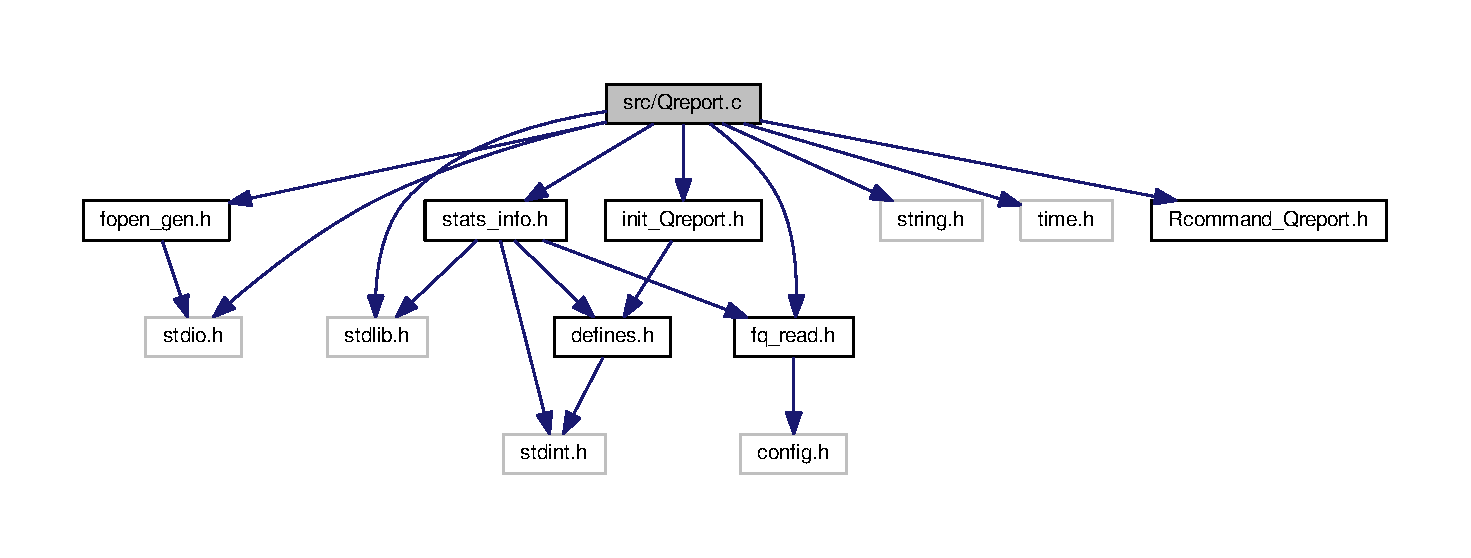
\includegraphics[width=350pt]{Qreport_8c__incl}
\end{center}
\end{figure}
\subsection*{Macros}
\begin{DoxyCompactItemize}
\item 
\#define \hyperlink{Qreport_8c_a4419cb9bb22330d00cfd4727a05060dd}{B\+\_\+\+L\+E\+N}~131072
\end{DoxyCompactItemize}
\subsection*{Functions}
\begin{DoxyCompactItemize}
\item 
\hypertarget{Qreport_8c_a0ddf1224851353fc92bfbff6f499fa97}{int \hyperlink{Qreport_8c_a0ddf1224851353fc92bfbff6f499fa97}{main} (int argc, char $\ast$argv\mbox{[}$\,$\mbox{]})}\label{Qreport_8c_a0ddf1224851353fc92bfbff6f499fa97}

\begin{DoxyCompactList}\small\item\em Qreport main function. \end{DoxyCompactList}\end{DoxyCompactItemize}
\subsection*{Variables}
\begin{DoxyCompactItemize}
\item 
\hyperlink{init__Qreport_8h_a883b1b3db368b84ab55f011bbb41bc80}{Iparam\+\_\+\+Qreport} \hyperlink{Qreport_8c_a5c6527d396580d559cfd1916fc959e23}{par\+\_\+\+Q\+R}
\end{DoxyCompactItemize}


\subsection{Detailed Description}
Q\+Report main function. 

\begin{DoxyAuthor}{Author}
Paula Perez \href{mailto:paulaperezrubio@gmail.com}{\tt paulaperezrubio@gmail.\+com} 
\end{DoxyAuthor}
\begin{DoxyDate}{Date}
03.\+08.\+2017 This file contains the quality report main function. It reads a fastq file and creates a html quality report. See R\+E\+A\+D\+M\+E\+\_\+\+Qreport.\+md for more details. 
\end{DoxyDate}


\subsection{Macro Definition Documentation}
\hypertarget{Qreport_8c_a4419cb9bb22330d00cfd4727a05060dd}{\index{Qreport.\+c@{Qreport.\+c}!B\+\_\+\+L\+E\+N@{B\+\_\+\+L\+E\+N}}
\index{B\+\_\+\+L\+E\+N@{B\+\_\+\+L\+E\+N}!Qreport.\+c@{Qreport.\+c}}
\subsubsection[{B\+\_\+\+L\+E\+N}]{\setlength{\rightskip}{0pt plus 5cm}\#define B\+\_\+\+L\+E\+N~131072}}\label{Qreport_8c_a4419cb9bb22330d00cfd4727a05060dd}
buffer size 

\subsection{Variable Documentation}
\hypertarget{Qreport_8c_a5c6527d396580d559cfd1916fc959e23}{\index{Qreport.\+c@{Qreport.\+c}!par\+\_\+\+Q\+R@{par\+\_\+\+Q\+R}}
\index{par\+\_\+\+Q\+R@{par\+\_\+\+Q\+R}!Qreport.\+c@{Qreport.\+c}}
\subsubsection[{par\+\_\+\+Q\+R}]{\setlength{\rightskip}{0pt plus 5cm}{\bf Iparam\+\_\+\+Qreport} par\+\_\+\+Q\+R}}\label{Qreport_8c_a5c6527d396580d559cfd1916fc959e23}
global variable\+: input parameters 
\hypertarget{Rcommand__Freport_8c}{\section{src/\+Rcommand\+\_\+\+Freport.c File Reference}
\label{Rcommand__Freport_8c}\index{src/\+Rcommand\+\_\+\+Freport.\+c@{src/\+Rcommand\+\_\+\+Freport.\+c}}
}


get Rscript command for Freport  


{\ttfamily \#include $<$stdio.\+h$>$}\\*
{\ttfamily \#include $<$unistd.\+h$>$}\\*
{\ttfamily \#include \char`\"{}Rcommand\+\_\+\+Freport.\+h\char`\"{}}\\*
{\ttfamily \#include \char`\"{}init\+\_\+\+Freport.\+h\char`\"{}}\\*
{\ttfamily \#include \char`\"{}defines.\+h\char`\"{}}\\*
{\ttfamily \#include \char`\"{}config.\+h\char`\"{}}\\*
Include dependency graph for Rcommand\+\_\+\+Freport.\+c\+:\nopagebreak
\begin{figure}[H]
\begin{center}
\leavevmode
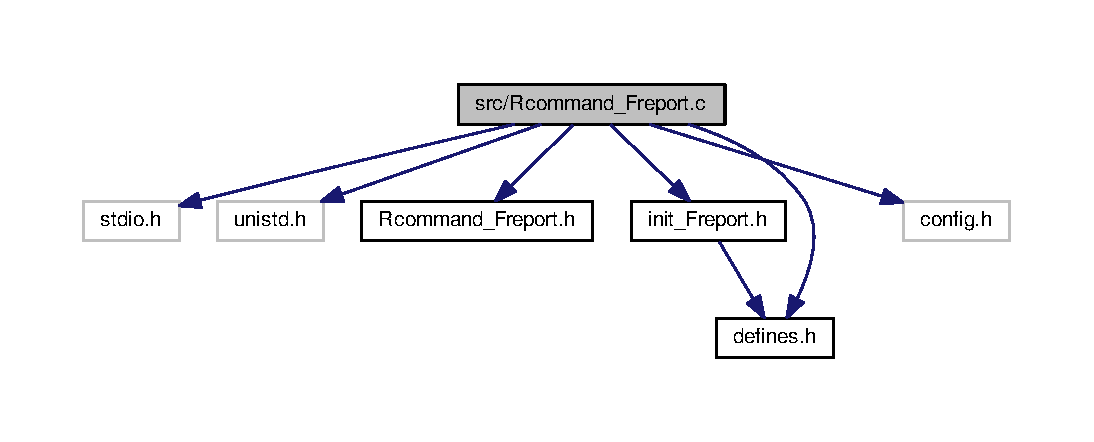
\includegraphics[width=350pt]{Rcommand__Freport_8c__incl}
\end{center}
\end{figure}
\subsection*{Functions}
\begin{DoxyCompactItemize}
\item 
\hypertarget{Rcommand__Freport_8c_a9ed436a2223e2511e514557c41cd86b8}{char $\ast$ \hyperlink{Rcommand__Freport_8c_a9ed436a2223e2511e514557c41cd86b8}{command\+\_\+\+Freport} ()}\label{Rcommand__Freport_8c_a9ed436a2223e2511e514557c41cd86b8}

\begin{DoxyCompactList}\small\item\em returns Rscript command that generates the summary report in html \end{DoxyCompactList}\end{DoxyCompactItemize}
\subsection*{Variables}
\begin{DoxyCompactItemize}
\item 
\hyperlink{init__Freport_8h_ad8a9800538d457840314d0c39b15c0db}{Iparam\+\_\+\+Freport} \hyperlink{Rcommand__Freport_8c_a953ecd02bc7b00cb35e50e8b0977221f}{par\+\_\+\+F\+R}
\end{DoxyCompactItemize}


\subsection{Detailed Description}
get Rscript command for Freport 

\begin{DoxyAuthor}{Author}
Paula Perez \href{mailto:paulaperezrubio@gmail.com}{\tt paulaperezrubio@gmail.\+com} 
\end{DoxyAuthor}
\begin{DoxyDate}{Date}
01.\+09.\+2017 
\end{DoxyDate}


\subsection{Variable Documentation}
\hypertarget{Rcommand__Freport_8c_a953ecd02bc7b00cb35e50e8b0977221f}{\index{Rcommand\+\_\+\+Freport.\+c@{Rcommand\+\_\+\+Freport.\+c}!par\+\_\+\+F\+R@{par\+\_\+\+F\+R}}
\index{par\+\_\+\+F\+R@{par\+\_\+\+F\+R}!Rcommand\+\_\+\+Freport.\+c@{Rcommand\+\_\+\+Freport.\+c}}
\subsubsection[{par\+\_\+\+F\+R}]{\setlength{\rightskip}{0pt plus 5cm}{\bf Iparam\+\_\+\+Freport} par\+\_\+\+F\+R}}\label{Rcommand__Freport_8c_a953ecd02bc7b00cb35e50e8b0977221f}
input parameters Freport 
\hypertarget{Rcommand__Qreport_8c}{}\section{src/\+Rcommand\+\_\+\+Qreport.c File Reference}
\label{Rcommand__Qreport_8c}\index{src/\+Rcommand\+\_\+\+Qreport.\+c@{src/\+Rcommand\+\_\+\+Qreport.\+c}}


get Rscript command for Qreport  


{\ttfamily \#include $<$stdio.\+h$>$}\newline
{\ttfamily \#include $<$stdlib.\+h$>$}\newline
{\ttfamily \#include $<$unistd.\+h$>$}\newline
{\ttfamily \#include \char`\"{}Rcommand\+\_\+\+Qreport.\+h\char`\"{}}\newline
{\ttfamily \#include \char`\"{}init\+\_\+\+Qreport.\+h\char`\"{}}\newline
{\ttfamily \#include \char`\"{}defines.\+h\char`\"{}}\newline
{\ttfamily \#include \char`\"{}config.\+h\char`\"{}}\newline
Include dependency graph for Rcommand\+\_\+\+Qreport.\+c\+:
\nopagebreak
\begin{figure}[H]
\begin{center}
\leavevmode
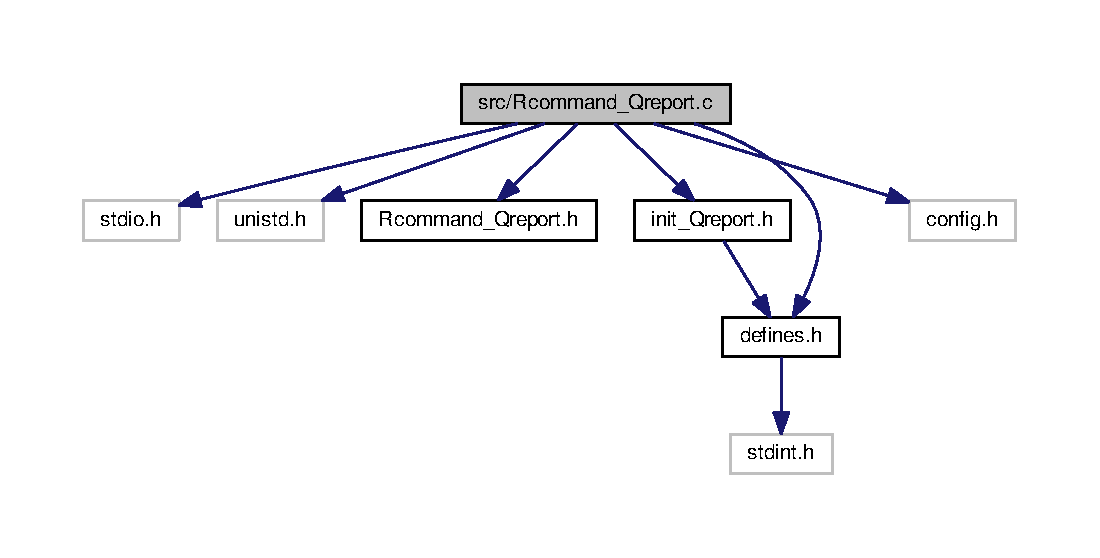
\includegraphics[width=350pt]{Rcommand__Qreport_8c__incl}
\end{center}
\end{figure}
\subsection*{Functions}
\begin{DoxyCompactItemize}
\item 
\mbox{\Hypertarget{Rcommand__Qreport_8c_a336345f346ab2a993022a0ca4862731c}\label{Rcommand__Qreport_8c_a336345f346ab2a993022a0ca4862731c}} 
char $\ast$ \mbox{\hyperlink{Rcommand__Qreport_8c_a336345f346ab2a993022a0ca4862731c}{command\+\_\+\+Qreport}} ()
\begin{DoxyCompactList}\small\item\em returns Rscript command that generates the quality report in html \end{DoxyCompactList}\end{DoxyCompactItemize}
\subsection*{Variables}
\begin{DoxyCompactItemize}
\item 
\mbox{\hyperlink{init__Qreport_8h_a883b1b3db368b84ab55f011bbb41bc80}{Iparam\+\_\+\+Qreport}} \mbox{\hyperlink{Rcommand__Qreport_8c_a5c6527d396580d559cfd1916fc959e23}{par\+\_\+\+QR}}
\end{DoxyCompactItemize}


\subsection{Detailed Description}
get Rscript command for Qreport 

\begin{DoxyAuthor}{Author}
Paula Perez \href{mailto:paulaperezrubio@gmail.com}{\tt paulaperezrubio@gmail.\+com} 
\end{DoxyAuthor}
\begin{DoxyDate}{Date}
07.\+08.\+2017 
\end{DoxyDate}


\subsection{Variable Documentation}
\mbox{\Hypertarget{Rcommand__Qreport_8c_a5c6527d396580d559cfd1916fc959e23}\label{Rcommand__Qreport_8c_a5c6527d396580d559cfd1916fc959e23}} 
\index{Rcommand\+\_\+\+Qreport.\+c@{Rcommand\+\_\+\+Qreport.\+c}!par\+\_\+\+QR@{par\+\_\+\+QR}}
\index{par\+\_\+\+QR@{par\+\_\+\+QR}!Rcommand\+\_\+\+Qreport.\+c@{Rcommand\+\_\+\+Qreport.\+c}}
\subsubsection{\texorpdfstring{par\+\_\+\+QR}{par\_QR}}
{\footnotesize\ttfamily \mbox{\hyperlink{init__Qreport_8h_a883b1b3db368b84ab55f011bbb41bc80}{Iparam\+\_\+\+Qreport}} par\+\_\+\+QR}

input parameters Qreport

global variable\+: input parameters for Qreport 
\hypertarget{Rcommand__Sreport_8c}{}\section{src/\+Rcommand\+\_\+\+Sreport.c File Reference}
\label{Rcommand__Sreport_8c}\index{src/\+Rcommand\+\_\+\+Sreport.\+c@{src/\+Rcommand\+\_\+\+Sreport.\+c}}


get Rscript command for Sreport  


{\ttfamily \#include $<$stdio.\+h$>$}\newline
{\ttfamily \#include $<$stdlib.\+h$>$}\newline
{\ttfamily \#include $<$unistd.\+h$>$}\newline
{\ttfamily \#include \char`\"{}Rcommand\+\_\+\+Sreport.\+h\char`\"{}}\newline
{\ttfamily \#include \char`\"{}init\+\_\+\+Sreport.\+h\char`\"{}}\newline
{\ttfamily \#include \char`\"{}defines.\+h\char`\"{}}\newline
{\ttfamily \#include \char`\"{}config.\+h\char`\"{}}\newline
Include dependency graph for Rcommand\+\_\+\+Sreport.\+c\+:
\nopagebreak
\begin{figure}[H]
\begin{center}
\leavevmode
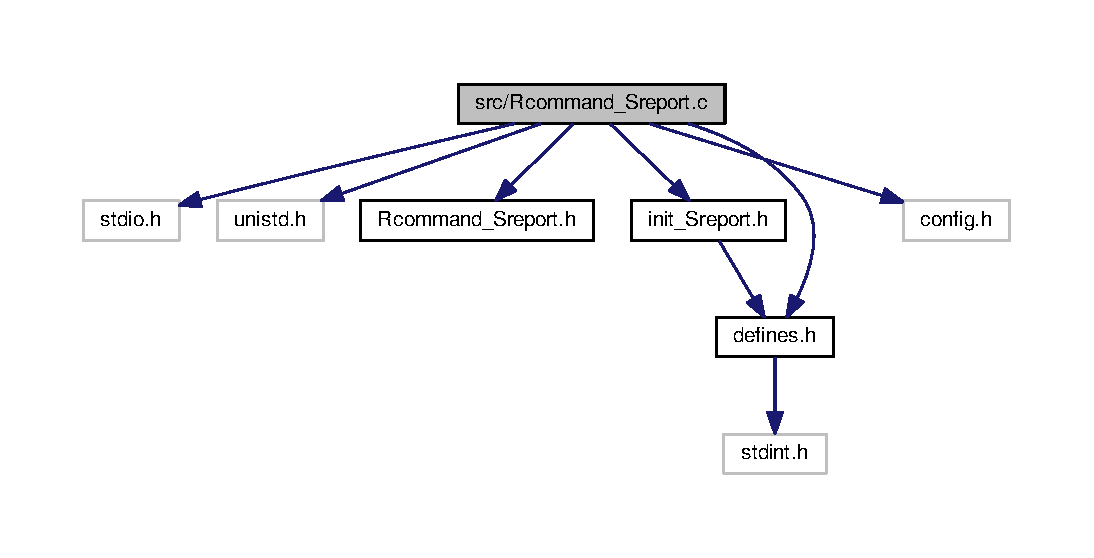
\includegraphics[width=350pt]{Rcommand__Sreport_8c__incl}
\end{center}
\end{figure}
\subsection*{Functions}
\begin{DoxyCompactItemize}
\item 
char $\ast$ \mbox{\hyperlink{Rcommand__Sreport_8c_a843ffc16afb438c7430da804efd8dfaf}{command\+\_\+\+Sreport}} ()
\begin{DoxyCompactList}\small\item\em returns Rscript command that generates the summary report in html \end{DoxyCompactList}\end{DoxyCompactItemize}
\subsection*{Variables}
\begin{DoxyCompactItemize}
\item 
\mbox{\hyperlink{init__Sreport_8h_ae7c35fd710a54db5b21f5c6b04fe9a5d}{Iparam\+\_\+\+Sreport}} \mbox{\hyperlink{Rcommand__Sreport_8c_aa230276b7e03d43430c998def780682e}{par\+\_\+\+SR}}
\end{DoxyCompactItemize}


\subsection{Detailed Description}
get Rscript command for Sreport 

\begin{DoxyAuthor}{Author}
Paula Perez \href{mailto:paulaperezrubio@gmail.com}{\tt paulaperezrubio@gmail.\+com} 
\end{DoxyAuthor}
\begin{DoxyDate}{Date}
09.\+08.\+2017 
\end{DoxyDate}


\subsection{Function Documentation}
\mbox{\Hypertarget{Rcommand__Sreport_8c_a843ffc16afb438c7430da804efd8dfaf}\label{Rcommand__Sreport_8c_a843ffc16afb438c7430da804efd8dfaf}} 
\index{Rcommand\+\_\+\+Sreport.\+c@{Rcommand\+\_\+\+Sreport.\+c}!command\+\_\+\+Sreport@{command\+\_\+\+Sreport}}
\index{command\+\_\+\+Sreport@{command\+\_\+\+Sreport}!Rcommand\+\_\+\+Sreport.\+c@{Rcommand\+\_\+\+Sreport.\+c}}
\subsubsection{\texorpdfstring{command\+\_\+\+Sreport()}{command\_Sreport()}}
{\footnotesize\ttfamily char$\ast$ command\+\_\+\+Sreport (\begin{DoxyParamCaption}{ }\end{DoxyParamCaption})}



returns Rscript command that generates the summary report in html 


\begin{DoxyCode}
# To run between quotation marks after:  Rscript\_RBioC -e (Rscript)
inputfolder = normalizePath( <par.SR.inputfolder>, mustWork = TRUE);
output = <par\_SR.outputfile>;
output\_file = gsub('.* /', '', output);
path = gsub('[^/]+$', '', output);
if (path != '') \{
  outputfile = paste0(normalizePath(path, mustWork = TRUE), '/', outputfile);
\} else \{
  outputfile = paste0(cwd, '/', output\_file); # cwd: current working dir
\}; 
rmarkdown::render(<par\_SR.Rmd\_file>, 
                  params = list(inputfolder = inputfolder, version= VERSION),
                  output\_file = output\_file)
\end{DoxyCode}
 

\subsection{Variable Documentation}
\mbox{\Hypertarget{Rcommand__Sreport_8c_aa230276b7e03d43430c998def780682e}\label{Rcommand__Sreport_8c_aa230276b7e03d43430c998def780682e}} 
\index{Rcommand\+\_\+\+Sreport.\+c@{Rcommand\+\_\+\+Sreport.\+c}!par\+\_\+\+SR@{par\+\_\+\+SR}}
\index{par\+\_\+\+SR@{par\+\_\+\+SR}!Rcommand\+\_\+\+Sreport.\+c@{Rcommand\+\_\+\+Sreport.\+c}}
\subsubsection{\texorpdfstring{par\+\_\+\+SR}{par\_SR}}
{\footnotesize\ttfamily \mbox{\hyperlink{init__Sreport_8h_ae7c35fd710a54db5b21f5c6b04fe9a5d}{Iparam\+\_\+\+Sreport}} par\+\_\+\+SR}

input parameters Sreport 
\hypertarget{Sreport_8c}{\section{src/\+Sreport.c File Reference}
\label{Sreport_8c}\index{src/\+Sreport.\+c@{src/\+Sreport.\+c}}
}


Sreport main function.  


{\ttfamily \#include $<$stdio.\+h$>$}\\*
{\ttfamily \#include $<$stdlib.\+h$>$}\\*
{\ttfamily \#include $<$time.\+h$>$}\\*
{\ttfamily \#include \char`\"{}init\+\_\+\+Sreport.\+h\char`\"{}}\\*
{\ttfamily \#include \char`\"{}Rcommand\+\_\+\+Sreport.\+h\char`\"{}}\\*
{\ttfamily \#include \char`\"{}config.\+h\char`\"{}}\\*
Include dependency graph for Sreport.\+c\+:\nopagebreak
\begin{figure}[H]
\begin{center}
\leavevmode
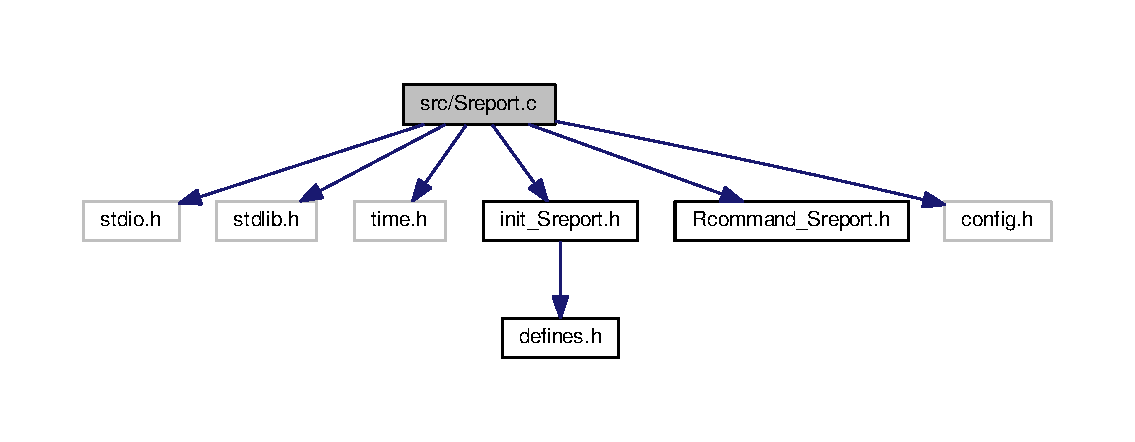
\includegraphics[width=350pt]{Sreport_8c__incl}
\end{center}
\end{figure}
\subsection*{Functions}
\begin{DoxyCompactItemize}
\item 
\hypertarget{Sreport_8c_a0ddf1224851353fc92bfbff6f499fa97}{int \hyperlink{Sreport_8c_a0ddf1224851353fc92bfbff6f499fa97}{main} (int argc, char $\ast$argv\mbox{[}$\,$\mbox{]})}\label{Sreport_8c_a0ddf1224851353fc92bfbff6f499fa97}

\begin{DoxyCompactList}\small\item\em Qreport main function. \end{DoxyCompactList}\end{DoxyCompactItemize}
\subsection*{Variables}
\begin{DoxyCompactItemize}
\item 
\hyperlink{init__Sreport_8h_ae7c35fd710a54db5b21f5c6b04fe9a5d}{Iparam\+\_\+\+Sreport} \hyperlink{Sreport_8c_aa230276b7e03d43430c998def780682e}{par\+\_\+\+S\+R}
\end{DoxyCompactItemize}


\subsection{Detailed Description}
Sreport main function. 

\begin{DoxyAuthor}{Author}
Paula Perez \href{mailto:paulaperezrubio@gmail.com}{\tt paulaperezrubio@gmail.\+com} 
\end{DoxyAuthor}
\begin{DoxyDate}{Date}
09.\+08.\+2017 This file contains the summary report main function. Given a folder containing $\ast$bin as from Qreport output, Sreport generates a summary report in html format. See R\+E\+A\+D\+M\+E\+\_\+\+Sreport.\+md for more details. 
\end{DoxyDate}


\subsection{Variable Documentation}
\hypertarget{Sreport_8c_aa230276b7e03d43430c998def780682e}{\index{Sreport.\+c@{Sreport.\+c}!par\+\_\+\+S\+R@{par\+\_\+\+S\+R}}
\index{par\+\_\+\+S\+R@{par\+\_\+\+S\+R}!Sreport.\+c@{Sreport.\+c}}
\subsubsection[{par\+\_\+\+S\+R}]{\setlength{\rightskip}{0pt plus 5cm}{\bf Iparam\+\_\+\+Sreport} par\+\_\+\+S\+R}}\label{Sreport_8c_aa230276b7e03d43430c998def780682e}
input parameters Sreport 
\hypertarget{stats__info_8c}{\section{src/stats\+\_\+info.c File Reference}
\label{stats__info_8c}\index{src/stats\+\_\+info.\+c@{src/stats\+\_\+info.\+c}}
}


Construct the quality report variables and update them.  


{\ttfamily \#include $<$stdio.\+h$>$}\\*
{\ttfamily \#include $<$string.\+h$>$}\\*
{\ttfamily \#include \char`\"{}stats\+\_\+info.\+h\char`\"{}}\\*
{\ttfamily \#include \char`\"{}init\+\_\+\+Qreport.\+h\char`\"{}}\\*
{\ttfamily \#include \char`\"{}str\+\_\+manip.\+h\char`\"{}}\\*
Include dependency graph for stats\+\_\+info.\+c\+:\nopagebreak
\begin{figure}[H]
\begin{center}
\leavevmode
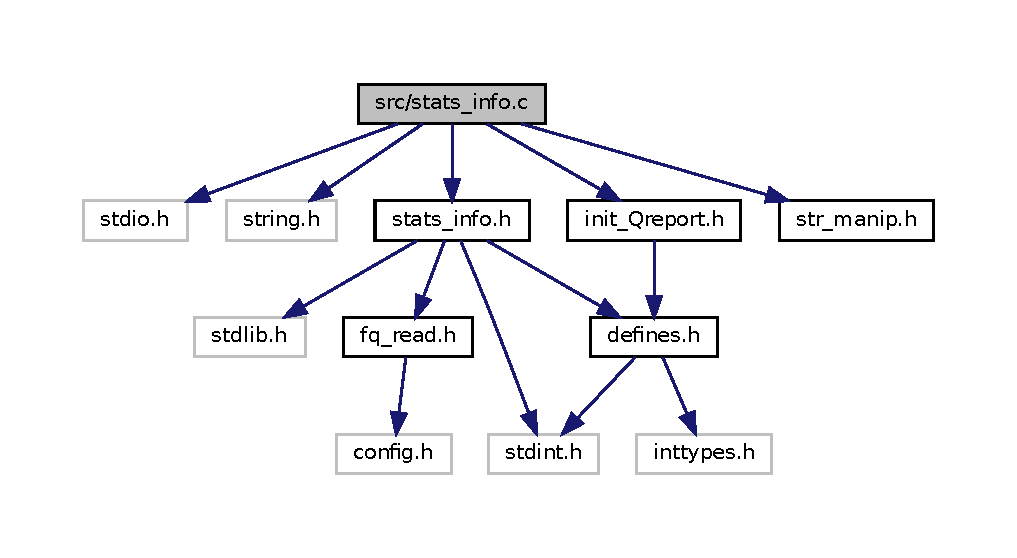
\includegraphics[width=350pt]{stats__info_8c__incl}
\end{center}
\end{figure}
\subsection*{Functions}
\begin{DoxyCompactItemize}
\item 
void \hyperlink{stats__info_8c_a5475bae263602449a0bb1af3ea112ad3}{get\+\_\+tile\+\_\+lane} (char $\ast$line1, int $\ast$tile, int $\ast$lane)
\begin{DoxyCompactList}\small\item\em get tile number from first line in fastq entry. \end{DoxyCompactList}\item 
\hypertarget{stats__info_8c_a398c4dad447f1384af6d620500788a0a}{static int \hyperlink{stats__info_8c_a398c4dad447f1384af6d620500788a0a}{belongsto} (int k, int $\ast$qual\+\_\+tags, int n\+Q)}\label{stats__info_8c_a398c4dad447f1384af6d620500788a0a}

\begin{DoxyCompactList}\small\item\em returns 1 if k is in qual\+\_\+tags, 0 otherwise. \end{DoxyCompactList}\item 
\hypertarget{stats__info_8c_ac4b64efac6b92ff63774c58b92d0fdb5}{static int \hyperlink{stats__info_8c_ac4b64efac6b92ff63774c58b92d0fdb5}{cmpfunc} (const void $\ast$a, const void $\ast$b)}\label{stats__info_8c_ac4b64efac6b92ff63774c58b92d0fdb5}

\begin{DoxyCompactList}\small\item\em comparison function for qsort \end{DoxyCompactList}\item 
void \hyperlink{stats__info_8c_a5c125debcca38ba396c6c01ecbc3dd5d}{init\+\_\+info} (\hyperlink{stats__info_8h_a2671cb2f7634ad56ed3dc27446796ef1}{Info} $\ast$res)
\begin{DoxyCompactList}\small\item\em Initialization of a Info type. \end{DoxyCompactList}\item 
\hypertarget{stats__info_8c_a3354d39b533bb35891251afdb5961a3a}{void \hyperlink{stats__info_8c_a3354d39b533bb35891251afdb5961a3a}{free\+\_\+info} (\hyperlink{stats__info_8h_a2671cb2f7634ad56ed3dc27446796ef1}{Info} $\ast$res)}\label{stats__info_8c_a3354d39b533bb35891251afdb5961a3a}

\begin{DoxyCompactList}\small\item\em frees allocated memory in Info \end{DoxyCompactList}\item 
\hypertarget{stats__info_8c_a7815bd5c300f89c99b539fa3e4c4f776}{void \hyperlink{stats__info_8c_a7815bd5c300f89c99b539fa3e4c4f776}{read\+\_\+info} (\hyperlink{stats__info_8h_a2671cb2f7634ad56ed3dc27446796ef1}{Info} $\ast$res, char $\ast$file)}\label{stats__info_8c_a7815bd5c300f89c99b539fa3e4c4f776}

\begin{DoxyCompactList}\small\item\em Read Info from binary file. \end{DoxyCompactList}\item 
\hypertarget{stats__info_8c_ae17b550d0328a66a4941b18f24f2a920}{void \hyperlink{stats__info_8c_ae17b550d0328a66a4941b18f24f2a920}{write\+\_\+info} (\hyperlink{stats__info_8h_a2671cb2f7634ad56ed3dc27446796ef1}{Info} $\ast$res, char $\ast$file)}\label{stats__info_8c_ae17b550d0328a66a4941b18f24f2a920}

\begin{DoxyCompactList}\small\item\em Write info to binary file. \end{DoxyCompactList}\item 
\hypertarget{stats__info_8c_a76d353cb30ac4cd4bc55362e7359976d}{void \hyperlink{stats__info_8c_a76d353cb30ac4cd4bc55362e7359976d}{print\+\_\+info} (\hyperlink{stats__info_8h_a2671cb2f7634ad56ed3dc27446796ef1}{Info} $\ast$res, char $\ast$infofile)}\label{stats__info_8c_a76d353cb30ac4cd4bc55362e7359976d}

\begin{DoxyCompactList}\small\item\em print Info to a textfile \end{DoxyCompactList}\item 
\hypertarget{stats__info_8c_a9ca0a2ed2eb78d9a9717b82efcfdcb1f}{void \hyperlink{stats__info_8c_a9ca0a2ed2eb78d9a9717b82efcfdcb1f}{get\+\_\+first\+\_\+tile} (\hyperlink{stats__info_8h_a2671cb2f7634ad56ed3dc27446796ef1}{Info} $\ast$res, \hyperlink{fq__read_8h_a9af37aa81397c9531c66863d4e97f034}{Fq\+\_\+read} $\ast$seq)}\label{stats__info_8c_a9ca0a2ed2eb78d9a9717b82efcfdcb1f}

\begin{DoxyCompactList}\small\item\em gets first tile \end{DoxyCompactList}\item 
\hypertarget{stats__info_8c_af599aaaf2eb242dcb6e9f44c0eb8c180}{void \hyperlink{stats__info_8c_af599aaaf2eb242dcb6e9f44c0eb8c180}{update\+\_\+info} (\hyperlink{stats__info_8h_a2671cb2f7634ad56ed3dc27446796ef1}{Info} $\ast$res, \hyperlink{fq__read_8h_a9af37aa81397c9531c66863d4e97f034}{Fq\+\_\+read} $\ast$seq)}\label{stats__info_8c_af599aaaf2eb242dcb6e9f44c0eb8c180}

\begin{DoxyCompactList}\small\item\em updates Info with Fq\+\_\+read \end{DoxyCompactList}\item 
int \hyperlink{stats__info_8c_a5bceee4c9ce4858a2e1a1022020f3051}{update\+\_\+\+A\+C\+G\+T\+\_\+counts} (uint64\+\_\+t $\ast$A\+C\+G\+T\+\_\+low, char A\+C\+G\+T)
\begin{DoxyCompactList}\small\item\em update, for current tile, A\+C\+G\+T counts. \end{DoxyCompactList}\item 
\hypertarget{stats__info_8c_a12859b5ec4a85f24df22833b2ddeee79}{void \hyperlink{stats__info_8c_a12859b5ec4a85f24df22833b2ddeee79}{update\+\_\+\+Q\+Pos\+Tile\+\_\+table} (\hyperlink{stats__info_8h_a2671cb2f7634ad56ed3dc27446796ef1}{Info} $\ast$res, \hyperlink{fq__read_8h_a9af37aa81397c9531c66863d4e97f034}{Fq\+\_\+read} $\ast$seq)}\label{stats__info_8c_a12859b5ec4a85f24df22833b2ddeee79}

\begin{DoxyCompactList}\small\item\em update Q\+Postile table \end{DoxyCompactList}\item 
\hypertarget{stats__info_8c_a0bf1e9e20a67a78adc88e500610b45f7}{void \hyperlink{stats__info_8c_a0bf1e9e20a67a78adc88e500610b45f7}{update\+\_\+\+A\+C\+G\+T\+\_\+pos} (uint64\+\_\+t $\ast$A\+C\+G\+T\+\_\+pos, \hyperlink{fq__read_8h_a9af37aa81397c9531c66863d4e97f034}{Fq\+\_\+read} $\ast$seq, int read\+\_\+len)}\label{stats__info_8c_a0bf1e9e20a67a78adc88e500610b45f7}

\begin{DoxyCompactList}\small\item\em update A\+C\+G\+T\+\_\+pos \end{DoxyCompactList}\item 
void \hyperlink{stats__info_8c_a8ca7ce52d36a35e78b8c0bde089aedcf}{resize\+\_\+info} (\hyperlink{stats__info_8h_a2671cb2f7634ad56ed3dc27446796ef1}{Info} $\ast$res)
\begin{DoxyCompactList}\small\item\em resize Info \end{DoxyCompactList}\end{DoxyCompactItemize}
\subsection*{Variables}
\begin{DoxyCompactItemize}
\item 
\hyperlink{init__Qreport_8h_a883b1b3db368b84ab55f011bbb41bc80}{Iparam\+\_\+\+Qreport} \hyperlink{stats__info_8c_a5c6527d396580d559cfd1916fc959e23}{par\+\_\+\+Q\+R}
\end{DoxyCompactItemize}


\subsection{Detailed Description}
Construct the quality report variables and update them. 

\begin{DoxyAuthor}{Author}
Paula Perez \href{mailto:paulaperezrubio@gmail.com}{\tt paulaperezrubio@gmail.\+com} 
\end{DoxyAuthor}
\begin{DoxyDate}{Date}
04.\+08.\+2017 
\end{DoxyDate}


\subsection{Function Documentation}
\hypertarget{stats__info_8c_a5475bae263602449a0bb1af3ea112ad3}{\index{stats\+\_\+info.\+c@{stats\+\_\+info.\+c}!get\+\_\+tile\+\_\+lane@{get\+\_\+tile\+\_\+lane}}
\index{get\+\_\+tile\+\_\+lane@{get\+\_\+tile\+\_\+lane}!stats\+\_\+info.\+c@{stats\+\_\+info.\+c}}
\subsubsection[{get\+\_\+tile\+\_\+lane}]{\setlength{\rightskip}{0pt plus 5cm}void get\+\_\+tile\+\_\+lane (
\begin{DoxyParamCaption}
\item[{char $\ast$}]{line1, }
\item[{int $\ast$}]{tile, }
\item[{int $\ast$}]{lane}
\end{DoxyParamCaption}
)}}\label{stats__info_8c_a5475bae263602449a0bb1af3ea112ad3}


get tile number from first line in fastq entry. 


\begin{DoxyParams}{Parameters}
{\em line1} & first line of a fastq entry \\
\hline
{\em tile} & int$\ast$ where the tile will be stored \\
\hline
{\em lane} & int$\ast$ where the lane will be stored \\
\hline
\end{DoxyParams}
\begin{DoxySeeAlso}{See also}
\href{http://wiki.christophchamp.com/index.php?title=FASTQ_format}{\tt http\+://wiki.\+christophchamp.\+com/index.\+php?title=\+F\+A\+S\+T\+Q\+\_\+format}
\end{DoxySeeAlso}
Only Illumina sequence identifiers are allowed. The line is inspected, and the number of '\+:' is obtained. The function exits with an error if the number of semicolons is different from 4 or 9. \hypertarget{stats__info_8c_a5c125debcca38ba396c6c01ecbc3dd5d}{\index{stats\+\_\+info.\+c@{stats\+\_\+info.\+c}!init\+\_\+info@{init\+\_\+info}}
\index{init\+\_\+info@{init\+\_\+info}!stats\+\_\+info.\+c@{stats\+\_\+info.\+c}}
\subsubsection[{init\+\_\+info}]{\setlength{\rightskip}{0pt plus 5cm}void init\+\_\+info (
\begin{DoxyParamCaption}
\item[{{\bf Info} $\ast$}]{res}
\end{DoxyParamCaption}
)}}\label{stats__info_8c_a5c125debcca38ba396c6c01ecbc3dd5d}


Initialization of a Info type. 

It sets\+: n\+Q, read\+\_\+len, ntiles, min\+Q and the dimensions of the arrays. Initializes the rest of the variables to zero and allocates memory to the arrays initializing them to 0 (calloc). \hypertarget{stats__info_8c_a8ca7ce52d36a35e78b8c0bde089aedcf}{\index{stats\+\_\+info.\+c@{stats\+\_\+info.\+c}!resize\+\_\+info@{resize\+\_\+info}}
\index{resize\+\_\+info@{resize\+\_\+info}!stats\+\_\+info.\+c@{stats\+\_\+info.\+c}}
\subsubsection[{resize\+\_\+info}]{\setlength{\rightskip}{0pt plus 5cm}void resize\+\_\+info (
\begin{DoxyParamCaption}
\item[{{\bf Info} $\ast$}]{res}
\end{DoxyParamCaption}
)}}\label{stats__info_8c_a8ca7ce52d36a35e78b8c0bde089aedcf}


resize Info 

At the end of the program, resize the structure Info, and adapt it to the actual number of tiles and the actual number of different quality values present. \hypertarget{stats__info_8c_a5bceee4c9ce4858a2e1a1022020f3051}{\index{stats\+\_\+info.\+c@{stats\+\_\+info.\+c}!update\+\_\+\+A\+C\+G\+T\+\_\+counts@{update\+\_\+\+A\+C\+G\+T\+\_\+counts}}
\index{update\+\_\+\+A\+C\+G\+T\+\_\+counts@{update\+\_\+\+A\+C\+G\+T\+\_\+counts}!stats\+\_\+info.\+c@{stats\+\_\+info.\+c}}
\subsubsection[{update\+\_\+\+A\+C\+G\+T\+\_\+counts}]{\setlength{\rightskip}{0pt plus 5cm}int update\+\_\+\+A\+C\+G\+T\+\_\+counts (
\begin{DoxyParamCaption}
\item[{uint64\+\_\+t $\ast$}]{A\+C\+G\+T\+\_\+low, }
\item[{char}]{A\+C\+G\+T}
\end{DoxyParamCaption}
)}}\label{stats__info_8c_a5bceee4c9ce4858a2e1a1022020f3051}


update, for current tile, A\+C\+G\+T counts. 

Makes update of A\+C\+G\+T counts for the current tile. Can be used with variables\+: low\+Q\+\_\+\+A\+C\+G\+T\+\_\+tile and A\+C\+G\+T\+\_\+tile 

\subsection{Variable Documentation}
\hypertarget{stats__info_8c_a5c6527d396580d559cfd1916fc959e23}{\index{stats\+\_\+info.\+c@{stats\+\_\+info.\+c}!par\+\_\+\+Q\+R@{par\+\_\+\+Q\+R}}
\index{par\+\_\+\+Q\+R@{par\+\_\+\+Q\+R}!stats\+\_\+info.\+c@{stats\+\_\+info.\+c}}
\subsubsection[{par\+\_\+\+Q\+R}]{\setlength{\rightskip}{0pt plus 5cm}{\bf Iparam\+\_\+\+Qreport} par\+\_\+\+Q\+R}}\label{stats__info_8c_a5c6527d396580d559cfd1916fc959e23}
global variable\+: input parameters for Qreport 
\hypertarget{str__manip_8c}{\section{src/str\+\_\+manip.c File Reference}
\label{str__manip_8c}\index{src/str\+\_\+manip.\+c@{src/str\+\_\+manip.\+c}}
}


functions that do string manipulation  


{\ttfamily \#include $<$stdio.\+h$>$}\\*
{\ttfamily \#include $<$stdlib.\+h$>$}\\*
{\ttfamily \#include $<$string.\+h$>$}\\*
{\ttfamily \#include \char`\"{}str\+\_\+manip.\+h\char`\"{}}\\*
Include dependency graph for str\+\_\+manip.\+c\+:\nopagebreak
\begin{figure}[H]
\begin{center}
\leavevmode
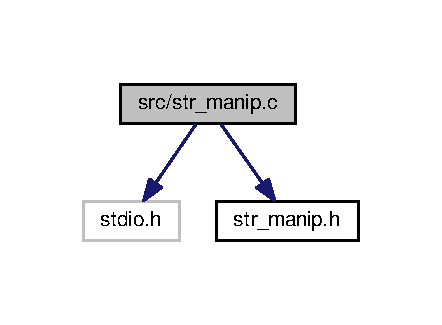
\includegraphics[width=346pt]{str__manip_8c__incl}
\end{center}
\end{figure}
\subsection*{Macros}
\begin{DoxyCompactItemize}
\item 
\#define \hyperlink{str__manip_8c_a416997b774a83987635e942c52952226}{\+\_\+\+\_\+isascii\+\_\+c}(c)~(((c) \& $\sim$0x7f) == 0)
\end{DoxyCompactItemize}
\subsection*{Functions}
\begin{DoxyCompactItemize}
\item 
\hypertarget{str__manip_8c_a15e8cbc96aa4cea159dbc59d1c01ffaa}{int \hyperlink{str__manip_8c_a15e8cbc96aa4cea159dbc59d1c01ffaa}{str\+\_\+isascii} (char $\ast$s)}\label{str__manip_8c_a15e8cbc96aa4cea159dbc59d1c01ffaa}

\begin{DoxyCompactList}\small\item\em return nonzero iff all elements in the string are in the A\+S\+C\+I\+I set. \end{DoxyCompactList}\item 
int \hyperlink{str__manip_8c_a8108ab52dfbc1af644bf7682c1bbe33f}{strindex} (char $\ast$s, char $\ast$t)
\begin{DoxyCompactList}\small\item\em returns index of t in s (start, first occurence) \end{DoxyCompactList}\item 
\hypertarget{str__manip_8c_a9790090291ece4c0a93c6c337dd528c1}{int \hyperlink{str__manip_8c_a9790090291ece4c0a93c6c337dd528c1}{count\+\_\+char} (char $\ast$str, char sep)}\label{str__manip_8c_a9790090291ece4c0a93c6c337dd528c1}

\begin{DoxyCompactList}\small\item\em returns the \# of occurences of char c in string s \end{DoxyCompactList}\item 
int \hyperlink{str__manip_8c_adc6cfcce267d36f0d09ecc6948d25747}{strindex\+C} (char $\ast$s, char sep)
\begin{DoxyCompactList}\small\item\em returns index of t in s (start, first occurence) \end{DoxyCompactList}\item 
\hyperlink{str__manip_8h_aeff63a40ce3fff0c51bd207baeba2013}{Split} \hyperlink{str__manip_8c_a245675aede3b8bedd8ce6c8c2aa70ec0}{strsplit} (char $\ast$str, char sep)
\begin{DoxyCompactList}\small\item\em Separates strings by a separator. \end{DoxyCompactList}\end{DoxyCompactItemize}


\subsection{Detailed Description}
functions that do string manipulation 

\begin{DoxyAuthor}{Author}
Paula Perez \href{mailto:paulaperezrubio@gmail.com}{\tt paulaperezrubio@gmail.\+com} 
\end{DoxyAuthor}
\begin{DoxyDate}{Date}
03.\+08.\+2017 
\end{DoxyDate}


\subsection{Macro Definition Documentation}
\hypertarget{str__manip_8c_a416997b774a83987635e942c52952226}{\index{str\+\_\+manip.\+c@{str\+\_\+manip.\+c}!\+\_\+\+\_\+isascii\+\_\+c@{\+\_\+\+\_\+isascii\+\_\+c}}
\index{\+\_\+\+\_\+isascii\+\_\+c@{\+\_\+\+\_\+isascii\+\_\+c}!str\+\_\+manip.\+c@{str\+\_\+manip.\+c}}
\subsubsection[{\+\_\+\+\_\+isascii\+\_\+c}]{\setlength{\rightskip}{0pt plus 5cm}\#define \+\_\+\+\_\+isascii\+\_\+c(
\begin{DoxyParamCaption}
\item[{}]{c}
\end{DoxyParamCaption}
)~(((c) \& $\sim$0x7f) == 0)}}\label{str__manip_8c_a416997b774a83987635e942c52952226}
If C is a 7 bit value. 

\subsection{Function Documentation}
\hypertarget{str__manip_8c_a8108ab52dfbc1af644bf7682c1bbe33f}{\index{str\+\_\+manip.\+c@{str\+\_\+manip.\+c}!strindex@{strindex}}
\index{strindex@{strindex}!str\+\_\+manip.\+c@{str\+\_\+manip.\+c}}
\subsubsection[{strindex}]{\setlength{\rightskip}{0pt plus 5cm}int strindex (
\begin{DoxyParamCaption}
\item[{char $\ast$}]{s, }
\item[{char $\ast$}]{t}
\end{DoxyParamCaption}
)}}\label{str__manip_8c_a8108ab52dfbc1af644bf7682c1bbe33f}


returns index of t in s (start, first occurence) 


\begin{DoxyParams}{Parameters}
{\em s} & string to be checked. \\
\hline
{\em t} & substring to be found in s. \\
\hline
\end{DoxyParams}
\hypertarget{str__manip_8c_adc6cfcce267d36f0d09ecc6948d25747}{\index{str\+\_\+manip.\+c@{str\+\_\+manip.\+c}!strindex\+C@{strindex\+C}}
\index{strindex\+C@{strindex\+C}!str\+\_\+manip.\+c@{str\+\_\+manip.\+c}}
\subsubsection[{strindex\+C}]{\setlength{\rightskip}{0pt plus 5cm}int strindex\+C (
\begin{DoxyParamCaption}
\item[{char $\ast$}]{s, }
\item[{char}]{sep}
\end{DoxyParamCaption}
)}}\label{str__manip_8c_adc6cfcce267d36f0d09ecc6948d25747}


returns index of t in s (start, first occurence) 


\begin{DoxyParams}{Parameters}
{\em s} & string to be checked. \\
\hline
{\em sep} & char, separator \\
\hline
\end{DoxyParams}
\hypertarget{str__manip_8c_a245675aede3b8bedd8ce6c8c2aa70ec0}{\index{str\+\_\+manip.\+c@{str\+\_\+manip.\+c}!strsplit@{strsplit}}
\index{strsplit@{strsplit}!str\+\_\+manip.\+c@{str\+\_\+manip.\+c}}
\subsubsection[{strsplit}]{\setlength{\rightskip}{0pt plus 5cm}{\bf Split} strsplit (
\begin{DoxyParamCaption}
\item[{char $\ast$}]{str, }
\item[{char}]{sep}
\end{DoxyParamCaption}
)}}\label{str__manip_8c_a245675aede3b8bedd8ce6c8c2aa70ec0}


Separates strings by a separator. 


\begin{DoxyParams}{Parameters}
{\em str} & input string \\
\hline
{\em sep} & separator (char) \\
\hline
\end{DoxyParams}
\begin{DoxyReturn}{Returns}
array of strings containing the substrings in the input separated 
\end{DoxyReturn}

\hypertarget{tree_8c}{\section{src/tree.c File Reference}
\label{tree_8c}\index{src/tree.\+c@{src/tree.\+c}}
}


Construction of tree, check paths, write tree, read in tree.  


{\ttfamily \#include $<$limits.\+h$>$}\\*
{\ttfamily \#include $<$string.\+h$>$}\\*
{\ttfamily \#include $<$stdlib.\+h$>$}\\*
{\ttfamily \#include $<$stdio.\+h$>$}\\*
{\ttfamily \#include \char`\"{}tree.\+h\char`\"{}}\\*
{\ttfamily \#include \char`\"{}Lmer.\+h\char`\"{}}\\*
{\ttfamily \#include \char`\"{}fopen\+\_\+gen.\+h\char`\"{}}\\*
Include dependency graph for tree.\+c\+:
\nopagebreak
\begin{figure}[H]
\begin{center}
\leavevmode
\includegraphics[width=350pt]{tree_8c__incl}
\end{center}
\end{figure}
\subsection*{Functions}
\begin{DoxyCompactItemize}
\item 
\hyperlink{tree_8h_a6390a1d02010dee1843fa2b1263308c1}{Node} $\ast$ \hyperlink{tree_8c_a759333d12a4ed298504cc08c69a19a27}{get\+\_\+new\+\_\+pool} (\hyperlink{tree_8h_a50a06950fa1e82738ad9a6bd85914900}{Tree} $\ast$tree\+\_\+ptr)
\begin{DoxyCompactList}\small\item\em reallocs pool\+\_\+2\+D (++\+N\+P\+O\+O\+L\+\_\+2\+D) if all existing nodes have been used \end{DoxyCompactList}\item 
\hyperlink{tree_8h_a6390a1d02010dee1843fa2b1263308c1}{Node} $\ast$ \hyperlink{tree_8c_a407b006b6b9c55cc8ef07c670becce33}{new\+\_\+node\+\_\+buf} (\hyperlink{tree_8h_a50a06950fa1e82738ad9a6bd85914900}{Tree} $\ast$tree\+\_\+ptr)
\begin{DoxyCompactList}\small\item\em moves to the next node (allocating new memory if necessary) \end{DoxyCompactList}\item 
void \hyperlink{tree_8c_a9bf758d5738d90a332fcd04485853d84}{free\+\_\+all\+\_\+nodes} (\hyperlink{tree_8h_a50a06950fa1e82738ad9a6bd85914900}{Tree} $\ast$tree\+\_\+ptr)
\begin{DoxyCompactList}\small\item\em frees the whole tree structure \end{DoxyCompactList}\item 
\hypertarget{tree_8c_a3cd8ebe19e5c6e6b54771eede75c935b}{void \hyperlink{tree_8c_a3cd8ebe19e5c6e6b54771eede75c935b}{insert\+\_\+\+Lmer} (\hyperlink{tree_8h_a50a06950fa1e82738ad9a6bd85914900}{Tree} $\ast$tree\+\_\+ptr, char $\ast$Lmer)}\label{tree_8c_a3cd8ebe19e5c6e6b54771eede75c935b}

\begin{DoxyCompactList}\small\item\em Lmer insertion in the tree (depth L). \end{DoxyCompactList}\item 
\hypertarget{tree_8c_a5f428a722fa118b5f4684fd06401db9a}{void \hyperlink{tree_8c_a5f428a722fa118b5f4684fd06401db9a}{insert\+\_\+entry} (\hyperlink{tree_8h_a50a06950fa1e82738ad9a6bd85914900}{Tree} $\ast$tree\+\_\+ptr, \hyperlink{fa__read_8h_a8f68b28ad3a6c33fe1dd78d5ac044b30}{Fa\+\_\+entry} $\ast$entry)}\label{tree_8c_a5f428a722fa118b5f4684fd06401db9a}

\begin{DoxyCompactList}\small\item\em fasta entry insertion in the tree (depth L). \end{DoxyCompactList}\item 
\hyperlink{tree_8h_a50a06950fa1e82738ad9a6bd85914900}{Tree} $\ast$ \hyperlink{tree_8c_a3cec782fc1e0ae4063a34c641b463f89}{tree\+\_\+from\+\_\+fasta} (\hyperlink{fa__read_8h_a797328b16bc1c1088998cd164aafb09d}{Fa\+\_\+data} $\ast$fasta, int L)
\begin{DoxyCompactList}\small\item\em create Tree structure from fasta structure. \end{DoxyCompactList}\item 
double \hyperlink{tree_8c_a7ea4e8b262dc61c20d94b598bffab181}{check\+\_\+path} (\hyperlink{tree_8h_a50a06950fa1e82738ad9a6bd85914900}{Tree} $\ast$tree\+\_\+ptr, char $\ast$read, int Lread)
\begin{DoxyCompactList}\small\item\em checks if read is found in tree and outputs a score \end{DoxyCompactList}\item 
void \hyperlink{tree_8c_a3b6ea3f3ef0c84a182e93a58ea417aea}{save\+\_\+tree} (\hyperlink{tree_8h_a50a06950fa1e82738ad9a6bd85914900}{Tree} $\ast$tree\+\_\+ptr, char $\ast$filename)
\begin{DoxyCompactList}\small\item\em saves Tree to disk in filename \end{DoxyCompactList}\item 
\hyperlink{tree_8h_a50a06950fa1e82738ad9a6bd85914900}{Tree} $\ast$ \hyperlink{tree_8c_a58f15d601ef34104e008d0ff8cb28bee}{read\+\_\+tree} (char $\ast$filename)
\begin{DoxyCompactList}\small\item\em read tree from file \end{DoxyCompactList}\end{DoxyCompactItemize}
\subsection*{Variables}
\begin{DoxyCompactItemize}
\item 
uint64\+\_\+t \hyperlink{tree_8c_a1f18264718e0b1b1be5a1f0ee64431e4}{alloc\+\_\+mem}
\end{DoxyCompactItemize}


\subsection{Detailed Description}
Construction of tree, check paths, write tree, read in tree. 

\begin{DoxyAuthor}{Author}
Paula Perez \href{mailto:paulaperezrubio@gmail.com}{\tt paulaperezrubio@gmail.\+com} 
\end{DoxyAuthor}
\begin{DoxyDate}{Date}
23.\+08.\+2017 
\end{DoxyDate}


\subsection{Function Documentation}
\hypertarget{tree_8c_a7ea4e8b262dc61c20d94b598bffab181}{\index{tree.\+c@{tree.\+c}!check\+\_\+path@{check\+\_\+path}}
\index{check\+\_\+path@{check\+\_\+path}!tree.\+c@{tree.\+c}}
\subsubsection[{check\+\_\+path}]{\setlength{\rightskip}{0pt plus 5cm}double check\+\_\+path (
\begin{DoxyParamCaption}
\item[{{\bf Tree} $\ast$}]{tree\+\_\+ptr, }
\item[{char $\ast$}]{read, }
\item[{int}]{Lread}
\end{DoxyParamCaption}
)}}\label{tree_8c_a7ea4e8b262dc61c20d94b598bffab181}


checks if read is found in tree and outputs a score 


\begin{DoxyParams}{Parameters}
{\em tree\+\_\+ptr} & pointer to Tree structure \\
\hline
{\em read} & Read or reverse complement \\
\hline
{\em Lread} & length of read \\
\hline
\end{DoxyParams}
\begin{DoxyReturn}{Returns}
score = (number of Lmers of reads found in read) / (Lread-\/\+L+1) 
\end{DoxyReturn}
\hypertarget{tree_8c_a9bf758d5738d90a332fcd04485853d84}{\index{tree.\+c@{tree.\+c}!free\+\_\+all\+\_\+nodes@{free\+\_\+all\+\_\+nodes}}
\index{free\+\_\+all\+\_\+nodes@{free\+\_\+all\+\_\+nodes}!tree.\+c@{tree.\+c}}
\subsubsection[{free\+\_\+all\+\_\+nodes}]{\setlength{\rightskip}{0pt plus 5cm}void free\+\_\+all\+\_\+nodes (
\begin{DoxyParamCaption}
\item[{{\bf Tree} $\ast$}]{tree\+\_\+ptr}
\end{DoxyParamCaption}
)}}\label{tree_8c_a9bf758d5738d90a332fcd04485853d84}


frees the whole tree structure 


\begin{DoxyParams}{Parameters}
{\em tree\+\_\+ptr} & pointer to Tree structure\\
\hline
\end{DoxyParams}
This function deallocates the memory allocated in a Tree structure. \hypertarget{tree_8c_a759333d12a4ed298504cc08c69a19a27}{\index{tree.\+c@{tree.\+c}!get\+\_\+new\+\_\+pool@{get\+\_\+new\+\_\+pool}}
\index{get\+\_\+new\+\_\+pool@{get\+\_\+new\+\_\+pool}!tree.\+c@{tree.\+c}}
\subsubsection[{get\+\_\+new\+\_\+pool}]{\setlength{\rightskip}{0pt plus 5cm}{\bf Node}$\ast$ get\+\_\+new\+\_\+pool (
\begin{DoxyParamCaption}
\item[{{\bf Tree} $\ast$}]{tree\+\_\+ptr}
\end{DoxyParamCaption}
)}}\label{tree_8c_a759333d12a4ed298504cc08c69a19a27}


reallocs pool\+\_\+2\+D (++\+N\+P\+O\+O\+L\+\_\+2\+D) if all existing nodes have been used 


\begin{DoxyParams}{Parameters}
{\em tree\+\_\+ptr} & pointer to Tree structure \\
\hline
\end{DoxyParams}
\hypertarget{tree_8c_a407b006b6b9c55cc8ef07c670becce33}{\index{tree.\+c@{tree.\+c}!new\+\_\+node\+\_\+buf@{new\+\_\+node\+\_\+buf}}
\index{new\+\_\+node\+\_\+buf@{new\+\_\+node\+\_\+buf}!tree.\+c@{tree.\+c}}
\subsubsection[{new\+\_\+node\+\_\+buf}]{\setlength{\rightskip}{0pt plus 5cm}{\bf Node}$\ast$ new\+\_\+node\+\_\+buf (
\begin{DoxyParamCaption}
\item[{{\bf Tree} $\ast$}]{tree\+\_\+ptr}
\end{DoxyParamCaption}
)}}\label{tree_8c_a407b006b6b9c55cc8ef07c670becce33}


moves to the next node (allocating new memory if necessary) 


\begin{DoxyParams}{Parameters}
{\em tree\+\_\+ptr} & pointer to Tree structure \\
\hline
\end{DoxyParams}
\begin{DoxyReturn}{Returns}
address to next node
\end{DoxyReturn}
The function checks if there are available nodes (information stored in the variable tree\+\_\+ptr -\/$>$ pool\+\_\+available) and goes to the next node. If there is no nodes left, it allocates a new pool\+\_\+1\+D, and if there is no room left in the outter dimension, it reallocates N\+P\+O\+O\+L\+\_\+2\+D more Node$\ast$'s. If the number of nodes reaches U\+I\+N\+T\+\_\+\+M\+A\+X, the program returns an error message and exits. \hypertarget{tree_8c_a58f15d601ef34104e008d0ff8cb28bee}{\index{tree.\+c@{tree.\+c}!read\+\_\+tree@{read\+\_\+tree}}
\index{read\+\_\+tree@{read\+\_\+tree}!tree.\+c@{tree.\+c}}
\subsubsection[{read\+\_\+tree}]{\setlength{\rightskip}{0pt plus 5cm}{\bf Tree}$\ast$ read\+\_\+tree (
\begin{DoxyParamCaption}
\item[{char $\ast$}]{filename}
\end{DoxyParamCaption}
)}}\label{tree_8c_a58f15d601ef34104e008d0ff8cb28bee}


read tree from file 


\begin{DoxyParams}{Parameters}
{\em filename} & string with the filename \\
\hline
\end{DoxyParams}
\begin{DoxyReturn}{Returns}
pointer to Tree structure
\end{DoxyReturn}
This function unwinds the process carried out in save\+\_\+tree and assigns addresses to the children of every given node. \hypertarget{tree_8c_a3b6ea3f3ef0c84a182e93a58ea417aea}{\index{tree.\+c@{tree.\+c}!save\+\_\+tree@{save\+\_\+tree}}
\index{save\+\_\+tree@{save\+\_\+tree}!tree.\+c@{tree.\+c}}
\subsubsection[{save\+\_\+tree}]{\setlength{\rightskip}{0pt plus 5cm}void save\+\_\+tree (
\begin{DoxyParamCaption}
\item[{{\bf Tree} $\ast$}]{tree\+\_\+ptr, }
\item[{char $\ast$}]{filename}
\end{DoxyParamCaption}
)}}\label{tree_8c_a3b6ea3f3ef0c84a182e93a58ea417aea}


saves Tree to disk in filename 


\begin{DoxyParams}{Parameters}
{\em tree\+\_\+ptr} & pointer to Tree structure \\
\hline
{\em filename} & string containing filename\\
\hline
\end{DoxyParams}
The tree structure is stored as follows\+: every address is stored in a uint32\+\_\+t (we are not allowing trees with more than U\+I\+N\+T\+\_\+\+M\+A\+X nodes). For every node, the addresses of the children are stored in the following fashion\+:
\begin{DoxyItemize}
\item If it is pointing to N\+U\+L\+L\+: 0.
\item Otherwise\+: i2, the index in the outer dimension of pool\+\_\+2\+D is identified, and the difference jump = pool\+\_\+2\+D\mbox{[}i\mbox{]}\mbox{[}j\mbox{]}.children\mbox{[}k\mbox{]} -\/ pool\+\_\+2\+D\mbox{[}i2\mbox{]} is computed. i2$\ast$\+N\+P\+O\+O\+L\+\_\+\+D1 + jump is then stored for child k. 
\end{DoxyItemize}\hypertarget{tree_8c_a3cec782fc1e0ae4063a34c641b463f89}{\index{tree.\+c@{tree.\+c}!tree\+\_\+from\+\_\+fasta@{tree\+\_\+from\+\_\+fasta}}
\index{tree\+\_\+from\+\_\+fasta@{tree\+\_\+from\+\_\+fasta}!tree.\+c@{tree.\+c}}
\subsubsection[{tree\+\_\+from\+\_\+fasta}]{\setlength{\rightskip}{0pt plus 5cm}{\bf Tree}$\ast$ tree\+\_\+from\+\_\+fasta (
\begin{DoxyParamCaption}
\item[{{\bf Fa\+\_\+data} $\ast$}]{fasta, }
\item[{int}]{L}
\end{DoxyParamCaption}
)}}\label{tree_8c_a3cec782fc1e0ae4063a34c641b463f89}


create Tree structure from fasta structure. 


\begin{DoxyParams}{Parameters}
{\em fasta} & pointer to fasta structure \\
\hline
{\em L} & tree length \\
\hline
\end{DoxyParams}


\subsection{Variable Documentation}
\hypertarget{tree_8c_a1f18264718e0b1b1be5a1f0ee64431e4}{\index{tree.\+c@{tree.\+c}!alloc\+\_\+mem@{alloc\+\_\+mem}}
\index{alloc\+\_\+mem@{alloc\+\_\+mem}!tree.\+c@{tree.\+c}}
\subsubsection[{alloc\+\_\+mem}]{\setlength{\rightskip}{0pt plus 5cm}uint64\+\_\+t alloc\+\_\+mem}}\label{tree_8c_a1f18264718e0b1b1be5a1f0ee64431e4}
global variable. Memory allocated in the heap. 
\hypertarget{trim_8c}{\section{src/trim.c File Reference}
\label{trim_8c}\index{src/trim.\+c@{src/trim.\+c}}
}


trims/filter sequences after Quality, N's contaminations.  


{\ttfamily \#include $<$string.\+h$>$}\\*
{\ttfamily \#include $<$stdlib.\+h$>$}\\*
{\ttfamily \#include \char`\"{}trim.\+h\char`\"{}}\\*
{\ttfamily \#include \char`\"{}str\+\_\+manip.\+h\char`\"{}}\\*
{\ttfamily \#include \char`\"{}defines.\+h\char`\"{}}\\*
{\ttfamily \#include \char`\"{}config.\+h\char`\"{}}\\*
{\ttfamily \#include \char`\"{}struct\+\_\+trim\+Filter.\+h\char`\"{}}\\*
Include dependency graph for trim.\+c\+:\nopagebreak
\begin{figure}[H]
\begin{center}
\leavevmode
\includegraphics[width=350pt]{trim_8c__incl}
\end{center}
\end{figure}
\subsection*{Macros}
\begin{DoxyCompactItemize}
\item 
\#define \hyperlink{trim_8c_aaeb5f4dc06b2ca1b46fa5212b6b8a203}{T\+R\+I\+M\+\_\+\+S\+T\+R\+I\+N\+G}~20
\end{DoxyCompactItemize}
\subsection*{Functions}
\begin{DoxyCompactItemize}
\item 
static int \hyperlink{trim_8c_aa1ba5f740cba7b39672dc588b9a5deb7}{no\+\_\+\+N} (\hyperlink{fq__read_8h_a9af37aa81397c9531c66863d4e97f034}{Fq\+\_\+read} $\ast$seq)
\begin{DoxyCompactList}\small\item\em checks if a sequence contains any non standard base callings (N's) \end{DoxyCompactList}\item 
static int \hyperlink{trim_8c_a7006063272037ceb080150136d24e898}{Nfree\+\_\+\+Lmer} (\hyperlink{fq__read_8h_a9af37aa81397c9531c66863d4e97f034}{Fq\+\_\+read} $\ast$seq, int min\+L)
\begin{DoxyCompactList}\small\item\em Finds the largest Nfree sub-\/seq and keeps it if larger than min\+L. \end{DoxyCompactList}\item 
static int \hyperlink{trim_8c_ae2aeb2e7303c53e2a10009ee4e20e40e}{Ntrim\+\_\+ends} (\hyperlink{fq__read_8h_a9af37aa81397c9531c66863d4e97f034}{Fq\+\_\+read} $\ast$seq, int min\+L)
\begin{DoxyCompactList}\small\item\em trims a read if N's are at the ends and the remaining sub-\/seq $>$= min\+L \end{DoxyCompactList}\item 
static int \hyperlink{trim_8c_ae11fa52547dfdb0cf2af554eafbba1fc}{no\+\_\+low\+Q} (\hyperlink{fq__read_8h_a9af37aa81397c9531c66863d4e97f034}{Fq\+\_\+read} $\ast$seq, int min\+Q)
\begin{DoxyCompactList}\small\item\em checks if a sequence contains low\+Q nucleotides \end{DoxyCompactList}\item 
static int \hyperlink{trim_8c_a03d11622e683d103cec196c42dd654dd}{Qtrim\+\_\+ends} (\hyperlink{fq__read_8h_a9af37aa81397c9531c66863d4e97f034}{Fq\+\_\+read} $\ast$seq, int min\+Q, int min\+L)
\begin{DoxyCompactList}\small\item\em trims a read if low\+Qs are at the ends and remaining sub-\/seq $>$= min\+L \end{DoxyCompactList}\item 
static int \hyperlink{trim_8c_af3167128b208288e71c0c50f15e66e89}{Qtrim\+\_\+frac} (\hyperlink{fq__read_8h_a9af37aa81397c9531c66863d4e97f034}{Fq\+\_\+read} $\ast$seq, int min\+Q, int nlow\+Q)
\begin{DoxyCompactList}\small\item\em accepts the sequence as is if there are less than nlow\+Q \end{DoxyCompactList}\item 
static int \hyperlink{trim_8c_aeef0fcb68dba0ae69ef81bd330a037ad}{Qtrim\+\_\+endsfrac} (\hyperlink{fq__read_8h_a9af37aa81397c9531c66863d4e97f034}{Fq\+\_\+read} $\ast$seq, int min\+Q, int min\+L, int nlow\+Q)
\begin{DoxyCompactList}\small\item\em trims the ends for low\+Q. The rest is kept if it contains $<$ nlow\+Q low\+Q \end{DoxyCompactList}\item 
int \hyperlink{trim_8c_ad2fbad2c77c70be922a30e940367cda7}{Qtrim\+\_\+global} (\hyperlink{fq__read_8h_a9af37aa81397c9531c66863d4e97f034}{Fq\+\_\+read} $\ast$seq, int left, int right, char type)
\begin{DoxyCompactList}\small\item\em trims left from the left and right from the right \end{DoxyCompactList}\item 
static int \hyperlink{trim_8c_a03005207176057abeac4d0ab60afbf93}{align\+\_\+uint32} (\hyperlink{fq__read_8h_a9af37aa81397c9531c66863d4e97f034}{Fq\+\_\+read} $\ast$seq, \hyperlink{adapters_8h_ad1465e8f3bc3d3b1fc010a1e72436c56}{Ad\+\_\+seq} $\ast$ptr\+\_\+adap, \hyperlink{defines_8h_abb452686968e48b67397da5f97445f5b}{bool} all)
\begin{DoxyCompactList}\small\item\em alignment search between a fq read, and an adapter sequence, with a seed of 8 nucleotides. \end{DoxyCompactList}\item 
static int \hyperlink{trim_8c_acb771cbd1c3867505712a6f302ec0d2d}{align\+\_\+uint64} (\hyperlink{fq__read_8h_a9af37aa81397c9531c66863d4e97f034}{Fq\+\_\+read} $\ast$seq, \hyperlink{adapters_8h_ad1465e8f3bc3d3b1fc010a1e72436c56}{Ad\+\_\+seq} $\ast$ptr\+\_\+adap)
\begin{DoxyCompactList}\small\item\em Alignment search between a fq read, and an adapter sequence, w with a seed of 8 nucleotides. \end{DoxyCompactList}\item 
int \hyperlink{trim_8c_aed995029d7181d69875b2dee0d7b6ce9}{trim\+\_\+adapter} (\hyperlink{fq__read_8h_a9af37aa81397c9531c66863d4e97f034}{Fq\+\_\+read} $\ast$seq, \hyperlink{adapters_8h_ad1465e8f3bc3d3b1fc010a1e72436c56}{Ad\+\_\+seq} $\ast$adap\+\_\+list)
\begin{DoxyCompactList}\small\item\em trims sequence based on presence of N nucleotides \end{DoxyCompactList}\item 
int \hyperlink{trim_8c_af23d3685193b624b72a6969a49903a97}{trim\+\_\+sequence\+N} (\hyperlink{fq__read_8h_a9af37aa81397c9531c66863d4e97f034}{Fq\+\_\+read} $\ast$seq)
\begin{DoxyCompactList}\small\item\em trims sequence based on presence of N nucleotides \end{DoxyCompactList}\item 
int \hyperlink{trim_8c_ae5ab2bb79068d8a7e0d72686c1f50320}{trim\+\_\+sequence\+Q} (\hyperlink{fq__read_8h_a9af37aa81397c9531c66863d4e97f034}{Fq\+\_\+read} $\ast$seq)
\begin{DoxyCompactList}\small\item\em trims sequence based on low\+Q base callings \end{DoxyCompactList}\item 
\hyperlink{defines_8h_abb452686968e48b67397da5f97445f5b}{bool} \hyperlink{trim_8c_a7e2b4015298659b7e21a80d4bb031e2f}{is\+\_\+read\+\_\+in\+Tree} (\hyperlink{tree_8h_a50a06950fa1e82738ad9a6bd85914900}{Tree} $\ast$tree\+\_\+ptr, \hyperlink{fq__read_8h_a9af37aa81397c9531c66863d4e97f034}{Fq\+\_\+read} $\ast$seq)
\begin{DoxyCompactList}\small\item\em check if Lread is contained in tree. It computes the score for the read and its reverse complement; if one ot them exceeds the user selected threshold, it returns true. Otherwise, it returns false. \end{DoxyCompactList}\item 
\hyperlink{defines_8h_abb452686968e48b67397da5f97445f5b}{bool} \hyperlink{trim_8c_a6206f2c21429fd2ff36010b71989696d}{is\+\_\+read\+\_\+in\+Bloom} (\hyperlink{bloom_8h_a6cb32cf059e8f4efd1ef80938d982836}{Bfilter} $\ast$ptr\+\_\+bf, \hyperlink{fq__read_8h_a9af37aa81397c9531c66863d4e97f034}{Fq\+\_\+read} $\ast$seq, \hyperlink{bloom_8h_a4bf3f34a321ce545e533d29ce363f569}{Bfkmer} $\ast$ptr\+\_\+bfkmer)
\begin{DoxyCompactList}\small\item\em checks if a read is in Bloom filter. It computes the score for the read and returns true if it exceeds the user selected threshold. Returns false othersise. \end{DoxyCompactList}\end{DoxyCompactItemize}
\subsection*{Variables}
\begin{DoxyCompactItemize}
\item 
int \hyperlink{trim_8c_a4716e1b3151ae984ab8b42b54e7abdd6}{Nencode}
\item 
\hyperlink{struct__trimFilter_8h_aff83806f1ff2b5f3609dc7d4c04b7c19}{Iparam\+\_\+trim\+Filter} \hyperlink{trim_8c_aed14b08f25fd6aa9a6cffb8c0074c953}{par\+\_\+\+T\+F}
\end{DoxyCompactItemize}


\subsection{Detailed Description}
trims/filter sequences after Quality, N's contaminations. 

\begin{DoxyAuthor}{Author}
Paula Perez \href{mailto:paulaperezrubio@gmail.com}{\tt paulaperezrubio@gmail.\+com} 
\end{DoxyAuthor}
\begin{DoxyDate}{Date}
24.\+08.\+2017 
\end{DoxyDate}


\subsection{Macro Definition Documentation}
\hypertarget{trim_8c_aaeb5f4dc06b2ca1b46fa5212b6b8a203}{\index{trim.\+c@{trim.\+c}!T\+R\+I\+M\+\_\+\+S\+T\+R\+I\+N\+G@{T\+R\+I\+M\+\_\+\+S\+T\+R\+I\+N\+G}}
\index{T\+R\+I\+M\+\_\+\+S\+T\+R\+I\+N\+G@{T\+R\+I\+M\+\_\+\+S\+T\+R\+I\+N\+G}!trim.\+c@{trim.\+c}}
\subsubsection[{T\+R\+I\+M\+\_\+\+S\+T\+R\+I\+N\+G}]{\setlength{\rightskip}{0pt plus 5cm}\#define T\+R\+I\+M\+\_\+\+S\+T\+R\+I\+N\+G~20}}\label{trim_8c_aaeb5f4dc06b2ca1b46fa5212b6b8a203}
maximal length of trimming info string. 

\subsection{Function Documentation}
\hypertarget{trim_8c_a03005207176057abeac4d0ab60afbf93}{\index{trim.\+c@{trim.\+c}!align\+\_\+uint32@{align\+\_\+uint32}}
\index{align\+\_\+uint32@{align\+\_\+uint32}!trim.\+c@{trim.\+c}}
\subsubsection[{align\+\_\+uint32}]{\setlength{\rightskip}{0pt plus 5cm}static int align\+\_\+uint32 (
\begin{DoxyParamCaption}
\item[{{\bf Fq\+\_\+read} $\ast$}]{seq, }
\item[{{\bf Ad\+\_\+seq} $\ast$}]{ptr\+\_\+adap, }
\item[{{\bf bool}}]{all}
\end{DoxyParamCaption}
)\hspace{0.3cm}{\ttfamily [static]}}}\label{trim_8c_a03005207176057abeac4d0ab60afbf93}


alignment search between a fq read, and an adapter sequence, with a seed of 8 nucleotides. 

This function checks whether there is adapter contamination in a given read. It works stand alone if the adapter is shorter than 16 nucleotides, and is called from align\+\_\+uint64 when no 16-\/nucleotides long seeds are found. The criteria are the same as in align\+\_\+uint64, the seed length being 8-\/nucleotides long instead of 16. See the {\bfseries align\+\_\+uint64} documentation for more details.


\begin{DoxyParams}{Parameters}
{\em seq} & pointer to {\bfseries Fq\+\_\+read} \\
\hline
{\em ptr\+\_\+adap} & pointer to {\bfseries Ad\+\_\+seq} \\
\hline
{\em all} & true if the whole read has to be sweeped, false if only the ends. When this function is called from align\+\_\+uint64, only the ends need to be considered. \\
\hline
\end{DoxyParams}
\begin{DoxyReturn}{Returns}
-\/1 error, 0 discarded, 1 accepted as is, 2 accepted and trimmed 
\end{DoxyReturn}
\begin{DoxyNote}{Note}
Global input parameters from par\+\_\+\+T\+F are also used 
\end{DoxyNote}
\begin{DoxySeeAlso}{See also}
\hyperlink{struct__trimFilter_8h_a3442d07a10a4ab75064687f3c244e370}{Adapter} 

\hyperlink{struct__trimFilter_8h_aff83806f1ff2b5f3609dc7d4c04b7c19}{Iparam\+\_\+trim\+Filter} 

\hyperlink{trim_8c_acb771cbd1c3867505712a6f302ec0d2d}{align\+\_\+uint64} 

\hyperlink{adapters_8h_a474bb2a439e8396fe33f6998af243eee}{pack\+\_\+adapter} 

\hyperlink{adapters_8h_adc47abb63194fec1a3ec9d83991a1340}{obtain\+\_\+score} 
\end{DoxySeeAlso}
\hypertarget{trim_8c_acb771cbd1c3867505712a6f302ec0d2d}{\index{trim.\+c@{trim.\+c}!align\+\_\+uint64@{align\+\_\+uint64}}
\index{align\+\_\+uint64@{align\+\_\+uint64}!trim.\+c@{trim.\+c}}
\subsubsection[{align\+\_\+uint64}]{\setlength{\rightskip}{0pt plus 5cm}static int align\+\_\+uint64 (
\begin{DoxyParamCaption}
\item[{{\bf Fq\+\_\+read} $\ast$}]{seq, }
\item[{{\bf Ad\+\_\+seq} $\ast$}]{ptr\+\_\+adap}
\end{DoxyParamCaption}
)\hspace{0.3cm}{\ttfamily [static]}}}\label{trim_8c_acb771cbd1c3867505712a6f302ec0d2d}


Alignment search between a fq read, and an adapter sequence, w with a seed of 8 nucleotides. 


\begin{DoxyParams}{Parameters}
{\em seq} & pointer to {\bfseries Fq\+\_\+read} \\
\hline
{\em ptr\+\_\+adap} & pointer to {\bfseries Ad\+\_\+seq} \\
\hline
\end{DoxyParams}
\begin{DoxyReturn}{Returns}
-\/1 error, 0 discarded, 1 accepted as is, 2 accepted and trimmed 
\end{DoxyReturn}
\begin{DoxyNote}{Note}
Global input parameters from par\+\_\+\+T\+F are used 
\end{DoxyNote}
\begin{DoxySeeAlso}{See also}
\hyperlink{struct__trimFilter_8h_a3442d07a10a4ab75064687f3c244e370}{Adapter} 

\hyperlink{struct__trimFilter_8h_aff83806f1ff2b5f3609dc7d4c04b7c19}{Iparam\+\_\+trim\+Filter} 

\hyperlink{trim_8c_a03005207176057abeac4d0ab60afbf93}{align\+\_\+uint32} 

\hyperlink{adapters_8h_a474bb2a439e8396fe33f6998af243eee}{pack\+\_\+adapter} 

\hyperlink{adapters_8h_adc47abb63194fec1a3ec9d83991a1340}{obtain\+\_\+score}
\end{DoxySeeAlso}
This function checks whether there is adapter contamination in a given read. We start by looking for 16-\/nucleotides long seeds, where a user defined number of mismatches is allowed. If found, a score is computed. If the score is larger than the user defined threshold and the number of matched nucleotides exceeds M\+I\+N\+\_\+\+N\+M\+A\+T\+C\+H\+E\+S (12), then the read is trimmed if the remaining part is longer than min\+L (user defined) and discarded otherwise. If no 16-\/nucleotides long seeds are found, we proceed with 8-\/nucleotides long seeds (see {\bfseries align\+\_\+uint32}) and apply the same criteria to trim/discard a read. A list of possible situations follows, to illustrate how it works (min\+L=25, mismatches=2)\+:


\begin{DoxyCode}
1 ADAPTER: CAAGCAGAAGACGGCATACGAG
2 REV\_COM: AGATCGGAAGAGCTCGTATGCC
3 
4 CASE1A:  CACAGTCGATCAGCGAGCAGGCATTCATGCTGAGATCGGAAGAGATCGTATG
5                                          ||||||||||||X|||----
6                                          AGATCGGAAGAGCTCGTATG
7          - Seed: 16 Nucleotides
8          - Return: 2, TRIMA:0:31
9 CASE1B:  CACATCATCGCTAGCTATCGATCGATCGATGCTATGCAAGATCGGAAGAGCT
10                                                ||||||||------
11                                                AGATCGGAAGAGCT
12          - Seed: 8 Nucleotides
13          - Return: 2, TRIMA:0:37
14 CASE1C:  CACATCATCGCTAGCTATCGATCGATCGATGCTATGCACGAAGATCGGAAGA
15                                                   ||||||||---
16                                                   AGATCGGAAGA
17          - Seed: 8 Nucleotides
18          - Return: 1, reason: Match length < 12
19 CASE2A:  CATACATCACGAGCTAGCTAGAGATCGGAAGAGCTCGTATGCCCAGCATCGA
20                                ||||||||||||||||------
21                                AGATCGGAAGAGCTCGTATGCC
22          - Seed: 16 Nucleotides
23          - Return: 0, reason: remaining read too short.
24 CASE2B:  CCACAGTACAATACATCACGAGCTAGCTAGAGATCGGAAGAGCTCGTATGCC
25                                        ||||||||||||||||||||||
26                                        AGATCGGAAGAGCTCGTATGCC
27          - Seed: 16 Nucleotides
28          - Return: 2, TRIMA:0:28
29 CASE3A:  TATGCCGTCTTCTGCTTGCAGTGCATGCTGATGCATGCTGCATGCTAGCTGC
30          ||||||||||||||||--
31          TATGCCGTCTTCTGCTTG
32          - Seed: 16 Nucleotides
33          - Return: 0, reason: remaining read too short
34 CASE3B:  CGTCTTCTGCTTGCCGATCGATGCTAGCTACGATCGTCGAGCTAGCTACGTG
35          ||||||||-----
36          CGTCTTCTGCTTG
37          - Seed: 8 Nucleotides
38          - Return: 0, reason: remaining read too short
39 CASE3C:  TCTTCTGCTTGCCGATCGATGCTAGCTACGATCGTCGAGCTAGCTACGTGCG
40          ||||||||---
41          TCTTCTGCTTG
42          - Seed: 8 Nucleotides
43          - Return: 1, reason: Match length < 12
\end{DoxyCode}
 \hypertarget{trim_8c_a6206f2c21429fd2ff36010b71989696d}{\index{trim.\+c@{trim.\+c}!is\+\_\+read\+\_\+in\+Bloom@{is\+\_\+read\+\_\+in\+Bloom}}
\index{is\+\_\+read\+\_\+in\+Bloom@{is\+\_\+read\+\_\+in\+Bloom}!trim.\+c@{trim.\+c}}
\subsubsection[{is\+\_\+read\+\_\+in\+Bloom}]{\setlength{\rightskip}{0pt plus 5cm}{\bf bool} is\+\_\+read\+\_\+in\+Bloom (
\begin{DoxyParamCaption}
\item[{{\bf Bfilter} $\ast$}]{ptr\+\_\+bf, }
\item[{{\bf Fq\+\_\+read} $\ast$}]{seq, }
\item[{{\bf Bfkmer} $\ast$}]{ptr\+\_\+bfkmer}
\end{DoxyParamCaption}
)}}\label{trim_8c_a6206f2c21429fd2ff36010b71989696d}


checks if a read is in Bloom filter. It computes the score for the read and returns true if it exceeds the user selected threshold. Returns false othersise. 


\begin{DoxyParams}{Parameters}
{\em ptr\+\_\+bf} & pointer to Bfilter \\
\hline
{\em seq} & fastq read \\
\hline
{\em ptr\+\_\+bfkmer} & pointer to Procs\+\_\+kmer structure (will store global) \\
\hline
\end{DoxyParams}
\begin{DoxyReturn}{Returns}
true if read was found, false otherwise 
\end{DoxyReturn}
\hypertarget{trim_8c_a7e2b4015298659b7e21a80d4bb031e2f}{\index{trim.\+c@{trim.\+c}!is\+\_\+read\+\_\+in\+Tree@{is\+\_\+read\+\_\+in\+Tree}}
\index{is\+\_\+read\+\_\+in\+Tree@{is\+\_\+read\+\_\+in\+Tree}!trim.\+c@{trim.\+c}}
\subsubsection[{is\+\_\+read\+\_\+in\+Tree}]{\setlength{\rightskip}{0pt plus 5cm}{\bf bool} is\+\_\+read\+\_\+in\+Tree (
\begin{DoxyParamCaption}
\item[{{\bf Tree} $\ast$}]{tree\+\_\+ptr, }
\item[{{\bf Fq\+\_\+read} $\ast$}]{seq}
\end{DoxyParamCaption}
)}}\label{trim_8c_a7e2b4015298659b7e21a80d4bb031e2f}


check if Lread is contained in tree. It computes the score for the read and its reverse complement; if one ot them exceeds the user selected threshold, it returns true. Otherwise, it returns false. 


\begin{DoxyParams}{Parameters}
{\em tree\+\_\+ptr} & pointer to Tree structure \\
\hline
{\em seq} & fastq read \\
\hline
\end{DoxyParams}
\begin{DoxyReturn}{Returns}
true if read was found, false otherwise 
\end{DoxyReturn}
\hypertarget{trim_8c_a7006063272037ceb080150136d24e898}{\index{trim.\+c@{trim.\+c}!Nfree\+\_\+\+Lmer@{Nfree\+\_\+\+Lmer}}
\index{Nfree\+\_\+\+Lmer@{Nfree\+\_\+\+Lmer}!trim.\+c@{trim.\+c}}
\subsubsection[{Nfree\+\_\+\+Lmer}]{\setlength{\rightskip}{0pt plus 5cm}static int Nfree\+\_\+\+Lmer (
\begin{DoxyParamCaption}
\item[{{\bf Fq\+\_\+read} $\ast$}]{seq, }
\item[{int}]{min\+L}
\end{DoxyParamCaption}
)\hspace{0.3cm}{\ttfamily [static]}}}\label{trim_8c_a7006063272037ceb080150136d24e898}


Finds the largest Nfree sub-\/seq and keeps it if larger than min\+L. 


\begin{DoxyParams}{Parameters}
{\em seq} & fastq read \\
\hline
{\em min\+L} & minimum accepted trimmed length \\
\hline
\end{DoxyParams}
\begin{DoxyReturn}{Returns}
0 if not used, 1 if accepted as is, 2 if accepted and trimmed 
\end{DoxyReturn}
\hypertarget{trim_8c_ae11fa52547dfdb0cf2af554eafbba1fc}{\index{trim.\+c@{trim.\+c}!no\+\_\+low\+Q@{no\+\_\+low\+Q}}
\index{no\+\_\+low\+Q@{no\+\_\+low\+Q}!trim.\+c@{trim.\+c}}
\subsubsection[{no\+\_\+low\+Q}]{\setlength{\rightskip}{0pt plus 5cm}static int no\+\_\+low\+Q (
\begin{DoxyParamCaption}
\item[{{\bf Fq\+\_\+read} $\ast$}]{seq, }
\item[{int}]{min\+Q}
\end{DoxyParamCaption}
)\hspace{0.3cm}{\ttfamily [static]}}}\label{trim_8c_ae11fa52547dfdb0cf2af554eafbba1fc}


checks if a sequence contains low\+Q nucleotides 


\begin{DoxyParams}{Parameters}
{\em seq} & fastq read \\
\hline
{\em min\+Q} & minimum accepted quality value \\
\hline
\end{DoxyParams}
\begin{DoxyReturn}{Returns}
0 if seq contains low\+Q nucleotides, 1 otherwise 
\end{DoxyReturn}
\hypertarget{trim_8c_aa1ba5f740cba7b39672dc588b9a5deb7}{\index{trim.\+c@{trim.\+c}!no\+\_\+\+N@{no\+\_\+\+N}}
\index{no\+\_\+\+N@{no\+\_\+\+N}!trim.\+c@{trim.\+c}}
\subsubsection[{no\+\_\+\+N}]{\setlength{\rightskip}{0pt plus 5cm}static int no\+\_\+\+N (
\begin{DoxyParamCaption}
\item[{{\bf Fq\+\_\+read} $\ast$}]{seq}
\end{DoxyParamCaption}
)\hspace{0.3cm}{\ttfamily [static]}}}\label{trim_8c_aa1ba5f740cba7b39672dc588b9a5deb7}


checks if a sequence contains any non standard base callings (N's) 

\begin{DoxyReturn}{Returns}
0 if no N's found, 1 if N's found
\end{DoxyReturn}
This function checks if any of the base callings in a given fastq read is different from A, C, G, T. Basically, any char different from the former ones is classified as N. \hypertarget{trim_8c_ae2aeb2e7303c53e2a10009ee4e20e40e}{\index{trim.\+c@{trim.\+c}!Ntrim\+\_\+ends@{Ntrim\+\_\+ends}}
\index{Ntrim\+\_\+ends@{Ntrim\+\_\+ends}!trim.\+c@{trim.\+c}}
\subsubsection[{Ntrim\+\_\+ends}]{\setlength{\rightskip}{0pt plus 5cm}static int Ntrim\+\_\+ends (
\begin{DoxyParamCaption}
\item[{{\bf Fq\+\_\+read} $\ast$}]{seq, }
\item[{int}]{min\+L}
\end{DoxyParamCaption}
)\hspace{0.3cm}{\ttfamily [static]}}}\label{trim_8c_ae2aeb2e7303c53e2a10009ee4e20e40e}


trims a read if N's are at the ends and the remaining sub-\/seq $>$= min\+L 


\begin{DoxyParams}{Parameters}
{\em seq} & fastq read \\
\hline
{\em min\+L} & minimum accepted trimmed length \\
\hline
\end{DoxyParams}
\begin{DoxyReturn}{Returns}
0 if not used, 1 no N's found, 2 if accepted and trimmed 
\end{DoxyReturn}
\hypertarget{trim_8c_a03d11622e683d103cec196c42dd654dd}{\index{trim.\+c@{trim.\+c}!Qtrim\+\_\+ends@{Qtrim\+\_\+ends}}
\index{Qtrim\+\_\+ends@{Qtrim\+\_\+ends}!trim.\+c@{trim.\+c}}
\subsubsection[{Qtrim\+\_\+ends}]{\setlength{\rightskip}{0pt plus 5cm}static int Qtrim\+\_\+ends (
\begin{DoxyParamCaption}
\item[{{\bf Fq\+\_\+read} $\ast$}]{seq, }
\item[{int}]{min\+Q, }
\item[{int}]{min\+L}
\end{DoxyParamCaption}
)\hspace{0.3cm}{\ttfamily [static]}}}\label{trim_8c_a03d11622e683d103cec196c42dd654dd}


trims a read if low\+Qs are at the ends and remaining sub-\/seq $>$= min\+L 


\begin{DoxyParams}{Parameters}
{\em seq} & fastq read \\
\hline
{\em min\+Q} & minimum accepted quality value \\
\hline
{\em min\+L} & minimum accepted trimmed length \\
\hline
\end{DoxyParams}
\begin{DoxyReturn}{Returns}
0 if not used, 1 if accepted as is, 2 if accepted and trimmed 
\end{DoxyReturn}
\hypertarget{trim_8c_aeef0fcb68dba0ae69ef81bd330a037ad}{\index{trim.\+c@{trim.\+c}!Qtrim\+\_\+endsfrac@{Qtrim\+\_\+endsfrac}}
\index{Qtrim\+\_\+endsfrac@{Qtrim\+\_\+endsfrac}!trim.\+c@{trim.\+c}}
\subsubsection[{Qtrim\+\_\+endsfrac}]{\setlength{\rightskip}{0pt plus 5cm}static int Qtrim\+\_\+endsfrac (
\begin{DoxyParamCaption}
\item[{{\bf Fq\+\_\+read} $\ast$}]{seq, }
\item[{int}]{min\+Q, }
\item[{int}]{min\+L, }
\item[{int}]{nlow\+Q}
\end{DoxyParamCaption}
)\hspace{0.3cm}{\ttfamily [static]}}}\label{trim_8c_aeef0fcb68dba0ae69ef81bd330a037ad}


trims the ends for low\+Q. The rest is kept if it contains $<$ nlow\+Q low\+Q 


\begin{DoxyParams}{Parameters}
{\em seq} & fastq read \\
\hline
{\em min\+Q} & minimum accepted quality value \\
\hline
{\em min\+L} & minimum accepted trimmed length \\
\hline
{\em nlow\+Q} & threshold on low\+Q nucleotides ($>$= N\+O\+T allowed) \\
\hline
\end{DoxyParams}
\begin{DoxyReturn}{Returns}
0 if not used, 1 if accepted as is
\end{DoxyReturn}
Trims the ends if there are low\+Q bases. From the remaining part, it counts how many low\+Q bases there are and keeps it if there are less than nlow\+Q. \hypertarget{trim_8c_af3167128b208288e71c0c50f15e66e89}{\index{trim.\+c@{trim.\+c}!Qtrim\+\_\+frac@{Qtrim\+\_\+frac}}
\index{Qtrim\+\_\+frac@{Qtrim\+\_\+frac}!trim.\+c@{trim.\+c}}
\subsubsection[{Qtrim\+\_\+frac}]{\setlength{\rightskip}{0pt plus 5cm}static int Qtrim\+\_\+frac (
\begin{DoxyParamCaption}
\item[{{\bf Fq\+\_\+read} $\ast$}]{seq, }
\item[{int}]{min\+Q, }
\item[{int}]{nlow\+Q}
\end{DoxyParamCaption}
)\hspace{0.3cm}{\ttfamily [static]}}}\label{trim_8c_af3167128b208288e71c0c50f15e66e89}


accepts the sequence as is if there are less than nlow\+Q 


\begin{DoxyParams}{Parameters}
{\em seq} & fastq read \\
\hline
{\em min\+Q} & minimum accepted quality value \\
\hline
{\em nlow\+Q} & threshold on low\+Q nucleotides ($>$= N\+O\+T allowed) \\
\hline
\end{DoxyParams}
\begin{DoxyReturn}{Returns}
0 if not used, 1 if accepted as is 
\end{DoxyReturn}
\hypertarget{trim_8c_ad2fbad2c77c70be922a30e940367cda7}{\index{trim.\+c@{trim.\+c}!Qtrim\+\_\+global@{Qtrim\+\_\+global}}
\index{Qtrim\+\_\+global@{Qtrim\+\_\+global}!trim.\+c@{trim.\+c}}
\subsubsection[{Qtrim\+\_\+global}]{\setlength{\rightskip}{0pt plus 5cm}int Qtrim\+\_\+global (
\begin{DoxyParamCaption}
\item[{{\bf Fq\+\_\+read} $\ast$}]{seq, }
\item[{int}]{left, }
\item[{int}]{right, }
\item[{char}]{type}
\end{DoxyParamCaption}
)}}\label{trim_8c_ad2fbad2c77c70be922a30e940367cda7}


trims left from the left and right from the right 


\begin{DoxyParams}{Parameters}
{\em seq} & fastq read \\
\hline
{\em left} & number of nucleotides to be trimmed from the left \\
\hline
{\em right} & number of nucleotides to be trimmed from the right \\
\hline
{\em type} & char indicating the type of trimming (Q,A). \\
\hline
\end{DoxyParams}
\begin{DoxyReturn}{Returns}
2, since they are all accepted and trim 
\end{DoxyReturn}
\hypertarget{trim_8c_aed995029d7181d69875b2dee0d7b6ce9}{\index{trim.\+c@{trim.\+c}!trim\+\_\+adapter@{trim\+\_\+adapter}}
\index{trim\+\_\+adapter@{trim\+\_\+adapter}!trim.\+c@{trim.\+c}}
\subsubsection[{trim\+\_\+adapter}]{\setlength{\rightskip}{0pt plus 5cm}int trim\+\_\+adapter (
\begin{DoxyParamCaption}
\item[{{\bf Fq\+\_\+read} $\ast$}]{seq, }
\item[{{\bf Ad\+\_\+seq} $\ast$}]{adap\+\_\+list}
\end{DoxyParamCaption}
)}}\label{trim_8c_aed995029d7181d69875b2dee0d7b6ce9}


trims sequence based on presence of N nucleotides 

if (adapter length $<$ 16) -\/$>$ search for seeds 8 nucleotides long else -\/$>$ search for seeds 16 nucleotides long if (seed found) -\/$>$ calculate score if score $>$ threshold -\/$>$ aligner found, trim / discard and exit. else -\/$>$ search for seeds 8 nucleotides long 
\begin{DoxyParams}{Parameters}
{\em seq} & pointer to {\bfseries Fq\+\_\+read} \\
\hline
{\em adap\+\_\+list} & array of {\bfseries Ad\+\_\+seq} \\
\hline
\end{DoxyParams}
\begin{DoxyReturn}{Returns}
-\/1 error, 0 discarded, 1 accepted as is, 2 accepted and trimmed 
\end{DoxyReturn}
\begin{DoxyNote}{Note}
Global input parameters from par\+\_\+\+T\+F are also used 
\end{DoxyNote}
\hypertarget{trim_8c_af23d3685193b624b72a6969a49903a97}{\index{trim.\+c@{trim.\+c}!trim\+\_\+sequence\+N@{trim\+\_\+sequence\+N}}
\index{trim\+\_\+sequence\+N@{trim\+\_\+sequence\+N}!trim.\+c@{trim.\+c}}
\subsubsection[{trim\+\_\+sequence\+N}]{\setlength{\rightskip}{0pt plus 5cm}int trim\+\_\+sequence\+N (
\begin{DoxyParamCaption}
\item[{{\bf Fq\+\_\+read} $\ast$}]{seq}
\end{DoxyParamCaption}
)}}\label{trim_8c_af23d3685193b624b72a6969a49903a97}


trims sequence based on presence of N nucleotides 


\begin{DoxyParams}{Parameters}
{\em seq} & fastq read \\
\hline
\end{DoxyParams}
\begin{DoxyReturn}{Returns}
-\/1 error, 0 discarded, 1 accepted as is, 2 accepted and trimmed
\end{DoxyReturn}
This function calls a different function depending on the method passed as input par\+\_\+\+T\+F.\+trim\+N\+:
\begin{DoxyItemize}
\item \hyperlink{defines_8h_a996bde01ecac342918f0a2c4e7ce7bd5}{N\+O(0)}\+: accepts it as is, (1),
\item \hyperlink{defines_8h_a1edd1ea8bddaf4d9c5eb3eae1ee1726a}{A\+L\+L(1)}\+: accepts it as is if N\+O N's found (1), rejects it otherwise (0),
\item \hyperlink{defines_8h_a052e72209cfac2ff9aa78294f0bebea8}{E\+N\+D\+S(2)}\+: trims the ends and accepts it if it is longer than min\+L (2 if trimming, 1 if no trimming), rejects it otherwise (0),
\item \hyperlink{defines_8h_a53529d9638a1d70f6e5989dedf4c2672}{S\+T\+R\+I\+P(3)}\+: finds the longest N-\/free subsequence and trims it if it is at least min\+L nucleotides long (2 if trimming, 1 if no N's are found), rejects it otherwise (0). 
\end{DoxyItemize}\hypertarget{trim_8c_ae5ab2bb79068d8a7e0d72686c1f50320}{\index{trim.\+c@{trim.\+c}!trim\+\_\+sequence\+Q@{trim\+\_\+sequence\+Q}}
\index{trim\+\_\+sequence\+Q@{trim\+\_\+sequence\+Q}!trim.\+c@{trim.\+c}}
\subsubsection[{trim\+\_\+sequence\+Q}]{\setlength{\rightskip}{0pt plus 5cm}int trim\+\_\+sequence\+Q (
\begin{DoxyParamCaption}
\item[{{\bf Fq\+\_\+read} $\ast$}]{seq}
\end{DoxyParamCaption}
)}}\label{trim_8c_ae5ab2bb79068d8a7e0d72686c1f50320}


trims sequence based on low\+Q base callings 


\begin{DoxyParams}{Parameters}
{\em seq} & fastq read \\
\hline
\end{DoxyParams}
\begin{DoxyReturn}{Returns}
-\/1 error, 0 discarded, 1 accepted as is, 2 accepted and trimmed
\end{DoxyReturn}
This function calls a different function depending on the method passed as input par\+\_\+\+T\+F.\+trim\+Q\+:
\begin{DoxyItemize}
\item \hyperlink{defines_8h_a996bde01ecac342918f0a2c4e7ce7bd5}{N\+O(0)}\+: accepts is as is , (1),
\item \hyperlink{defines_8h_a653af6bd29f56a2699de26a928820da7}{F\+R\+A\+C(1)}\+: accepts it if less than par\+\_\+\+T\+F.\+nlow\+Q are found (1), rejects it otherwise (0),
\item \hyperlink{defines_8h_a052e72209cfac2ff9aa78294f0bebea8}{E\+N\+D\+S(2)}\+: trims the ends and accepts it if it is longer than min\+L (2 if triming, 1 if no trimming), rejects it otherwise (0),
\item \hyperlink{defines_8h_abf0b71573c7ffc4f6746c24c9abc202a}{E\+N\+D\+S\+F\+R\+A\+C(3)}\+: trims the ends and accepts if the remaining sequence is at least min\+L bases long and if it contains less than nlow\+Q low\+Q nucleotides (2 if trimming, 1 if no trimming). Otherwise, it is rejected, (0).
\item \hyperlink{defines_8h_a3de33738fd3c7e77bffbcfaefc3e7645}{G\+L\+O\+B\+A\+L(4)}\+: it trims globally globleft nucleotides from the left and globright from the right, (returns 2). 
\end{DoxyItemize}

\subsection{Variable Documentation}
\hypertarget{trim_8c_a4716e1b3151ae984ab8b42b54e7abdd6}{\index{trim.\+c@{trim.\+c}!Nencode@{Nencode}}
\index{Nencode@{Nencode}!trim.\+c@{trim.\+c}}
\subsubsection[{Nencode}]{\setlength{\rightskip}{0pt plus 5cm}int Nencode}}\label{trim_8c_a4716e1b3151ae984ab8b42b54e7abdd6}
global variable. Encoding for N's(\textbackslash{}004, or \textbackslash{}005) \hypertarget{trim_8c_aed14b08f25fd6aa9a6cffb8c0074c953}{\index{trim.\+c@{trim.\+c}!par\+\_\+\+T\+F@{par\+\_\+\+T\+F}}
\index{par\+\_\+\+T\+F@{par\+\_\+\+T\+F}!trim.\+c@{trim.\+c}}
\subsubsection[{par\+\_\+\+T\+F}]{\setlength{\rightskip}{0pt plus 5cm}{\bf Iparam\+\_\+trim\+Filter} par\+\_\+\+T\+F}}\label{trim_8c_aed14b08f25fd6aa9a6cffb8c0074c953}
global variable\+: Input parameters trim\+Filter.

global variable\+: Input parameters of make\+Tree. 
\hypertarget{trimFilter_8c}{\section{src/trim\+Filter.c File Reference}
\label{trimFilter_8c}\index{src/trim\+Filter.\+c@{src/trim\+Filter.\+c}}
}


trim\+Filter main function  


{\ttfamily \#include $<$stdio.\+h$>$}\\*
{\ttfamily \#include $<$time.\+h$>$}\\*
{\ttfamily \#include $<$string.\+h$>$}\\*
{\ttfamily \#include $<$stdlib.\+h$>$}\\*
{\ttfamily \#include \char`\"{}fq\+\_\+read.\+h\char`\"{}}\\*
{\ttfamily \#include \char`\"{}fopen\+\_\+gen.\+h\char`\"{}}\\*
{\ttfamily \#include \char`\"{}config.\+h\char`\"{}}\\*
{\ttfamily \#include \char`\"{}defines.\+h\char`\"{}}\\*
{\ttfamily \#include \char`\"{}init\+\_\+trim\+Filter.\+h\char`\"{}}\\*
{\ttfamily \#include \char`\"{}io\+\_\+trim\+Filter.\+h\char`\"{}}\\*
{\ttfamily \#include \char`\"{}tree.\+h\char`\"{}}\\*
{\ttfamily \#include \char`\"{}trim.\+h\char`\"{}}\\*
Include dependency graph for trim\+Filter.\+c\+:
\nopagebreak
\begin{figure}[H]
\begin{center}
\leavevmode
\includegraphics[width=350pt]{trimFilter_8c__incl}
\end{center}
\end{figure}
\subsection*{Functions}
\begin{DoxyCompactItemize}
\item 
\hypertarget{trimFilter_8c_a0ddf1224851353fc92bfbff6f499fa97}{int \hyperlink{trimFilter_8c_a0ddf1224851353fc92bfbff6f499fa97}{main} (int argc, char $\ast$argv\mbox{[}$\,$\mbox{]})}\label{trimFilter_8c_a0ddf1224851353fc92bfbff6f499fa97}

\begin{DoxyCompactList}\small\item\em make\+Tree main function \end{DoxyCompactList}\end{DoxyCompactItemize}
\subsection*{Variables}
\begin{DoxyCompactItemize}
\item 
uint64\+\_\+t \hyperlink{trimFilter_8c_a1f18264718e0b1b1be5a1f0ee64431e4}{alloc\+\_\+mem} = 0
\item 
\hyperlink{init__trimFilter_8h_aff83806f1ff2b5f3609dc7d4c04b7c19}{Iparam\+\_\+trim\+Filter} \hyperlink{trimFilter_8c_aed14b08f25fd6aa9a6cffb8c0074c953}{par\+\_\+\+T\+F}
\end{DoxyCompactItemize}


\subsection{Detailed Description}
trim\+Filter main function 

\begin{DoxyAuthor}{Author}
Paula Perez \href{mailto:paulaperezrubio@gmail.com}{\tt paulaperezrubio@gmail.\+com} 
\end{DoxyAuthor}
\begin{DoxyDate}{Date}
25.\+08.\+2017 This file contains the trim\+Filter main function. B\+L\+A B\+L\+A See R\+E\+A\+D\+M\+E\+\_\+trim\+Filter.\+md for more details. 
\end{DoxyDate}


\subsection{Variable Documentation}
\hypertarget{trimFilter_8c_a1f18264718e0b1b1be5a1f0ee64431e4}{\index{trim\+Filter.\+c@{trim\+Filter.\+c}!alloc\+\_\+mem@{alloc\+\_\+mem}}
\index{alloc\+\_\+mem@{alloc\+\_\+mem}!trim\+Filter.\+c@{trim\+Filter.\+c}}
\subsubsection[{alloc\+\_\+mem}]{\setlength{\rightskip}{0pt plus 5cm}uint64\+\_\+t alloc\+\_\+mem = 0}}\label{trimFilter_8c_a1f18264718e0b1b1be5a1f0ee64431e4}
global variable. Memory allocated in the heap. \hypertarget{trimFilter_8c_aed14b08f25fd6aa9a6cffb8c0074c953}{\index{trim\+Filter.\+c@{trim\+Filter.\+c}!par\+\_\+\+T\+F@{par\+\_\+\+T\+F}}
\index{par\+\_\+\+T\+F@{par\+\_\+\+T\+F}!trim\+Filter.\+c@{trim\+Filter.\+c}}
\subsubsection[{par\+\_\+\+T\+F}]{\setlength{\rightskip}{0pt plus 5cm}{\bf Iparam\+\_\+trim\+Filter} par\+\_\+\+T\+F}}\label{trimFilter_8c_aed14b08f25fd6aa9a6cffb8c0074c953}
global variable\+: Input parameters of make\+Tree. 
%--- End generated contents ---

% Index
\newpage
\phantomsection
\addcontentsline{toc}{chapter}{Index}
\printindex

\end{document}
